\section{Eksperymenty}\label{sec:experiments}
W tym rozdziale opisane zostały eksperymenty przeprowadzone w celu zbadania testów wydajnościowych środowisk uruchomieniowych. Testy zostały przeprowadzone na jednym komputerze wyposażonym w system operacyjny Linux, co pozwoliło na zminimalizowanie wpływu innych czynników na wyniki testów.

Testy wykorzystują wszystkie możliwe funkcjonalności, które są zaimplementowane w danych środowiskach, dzięki czemu, testy te są odzwierciedleniem rzeczywistego zastosowania danego środowiska. Testy zostały wykonane w dwóch językach programowania: JavaScript oraz TypeScript. Zastosowanie tych języków pozwala na przetestowanie czasu potrzebnego do transpilacji kodu źródłowego do kodu maszynowego. 

\subsection{Algorytmy sortowania}
W celu zbadania wydajności danego środowiska uruchomieniowego, skonstruowana odpowiednie eksperymenty, które sprawdzają wydajność algorytmu sortowania. Wszystkie algorytmy sortowania zostały przetestowane dla każdego środowiska.

W tabeli \ref{tab:sorting_experiments} przedstawiono ilość iteracji oraz ilość elementów dla przeprowadzonych eksperymentów.

\begin{table}[H]
  \centering
  \caption{Parametry eksperymentów - algorytmy sortowania}
  \begin{tabular}{|c|c|}
    \hline
    \textbf{Liczba eksperymentów} & \textbf{Liczba elementów} \\ \hline
    100 & 1000 \\ \hline
    1000 & 1000 \\ \hline
    100 & 10000 \\ \hline
    1000 & 10000 \\ \hline
  \end{tabular}
  \label{tab:sorting_experiments}
\end{table}

\subsubsection{Wyniki - sortowanie bąbelkowe}
Na rysunku \ref{fig:bubble_sorting_e1} przedstawiono wyniki eksperymentów dla algorytmu sortowania bąbelkowego dla 100 iteracji i 1000 elementów napisanego w języku JavaScript. Na wykresie przedstawiono czas wykonania jednorazowego testu w milisekundach oraz ilość zajmowanej pamięci w kilobajtach (kB).

\begin{figure}[H]
  \centering
  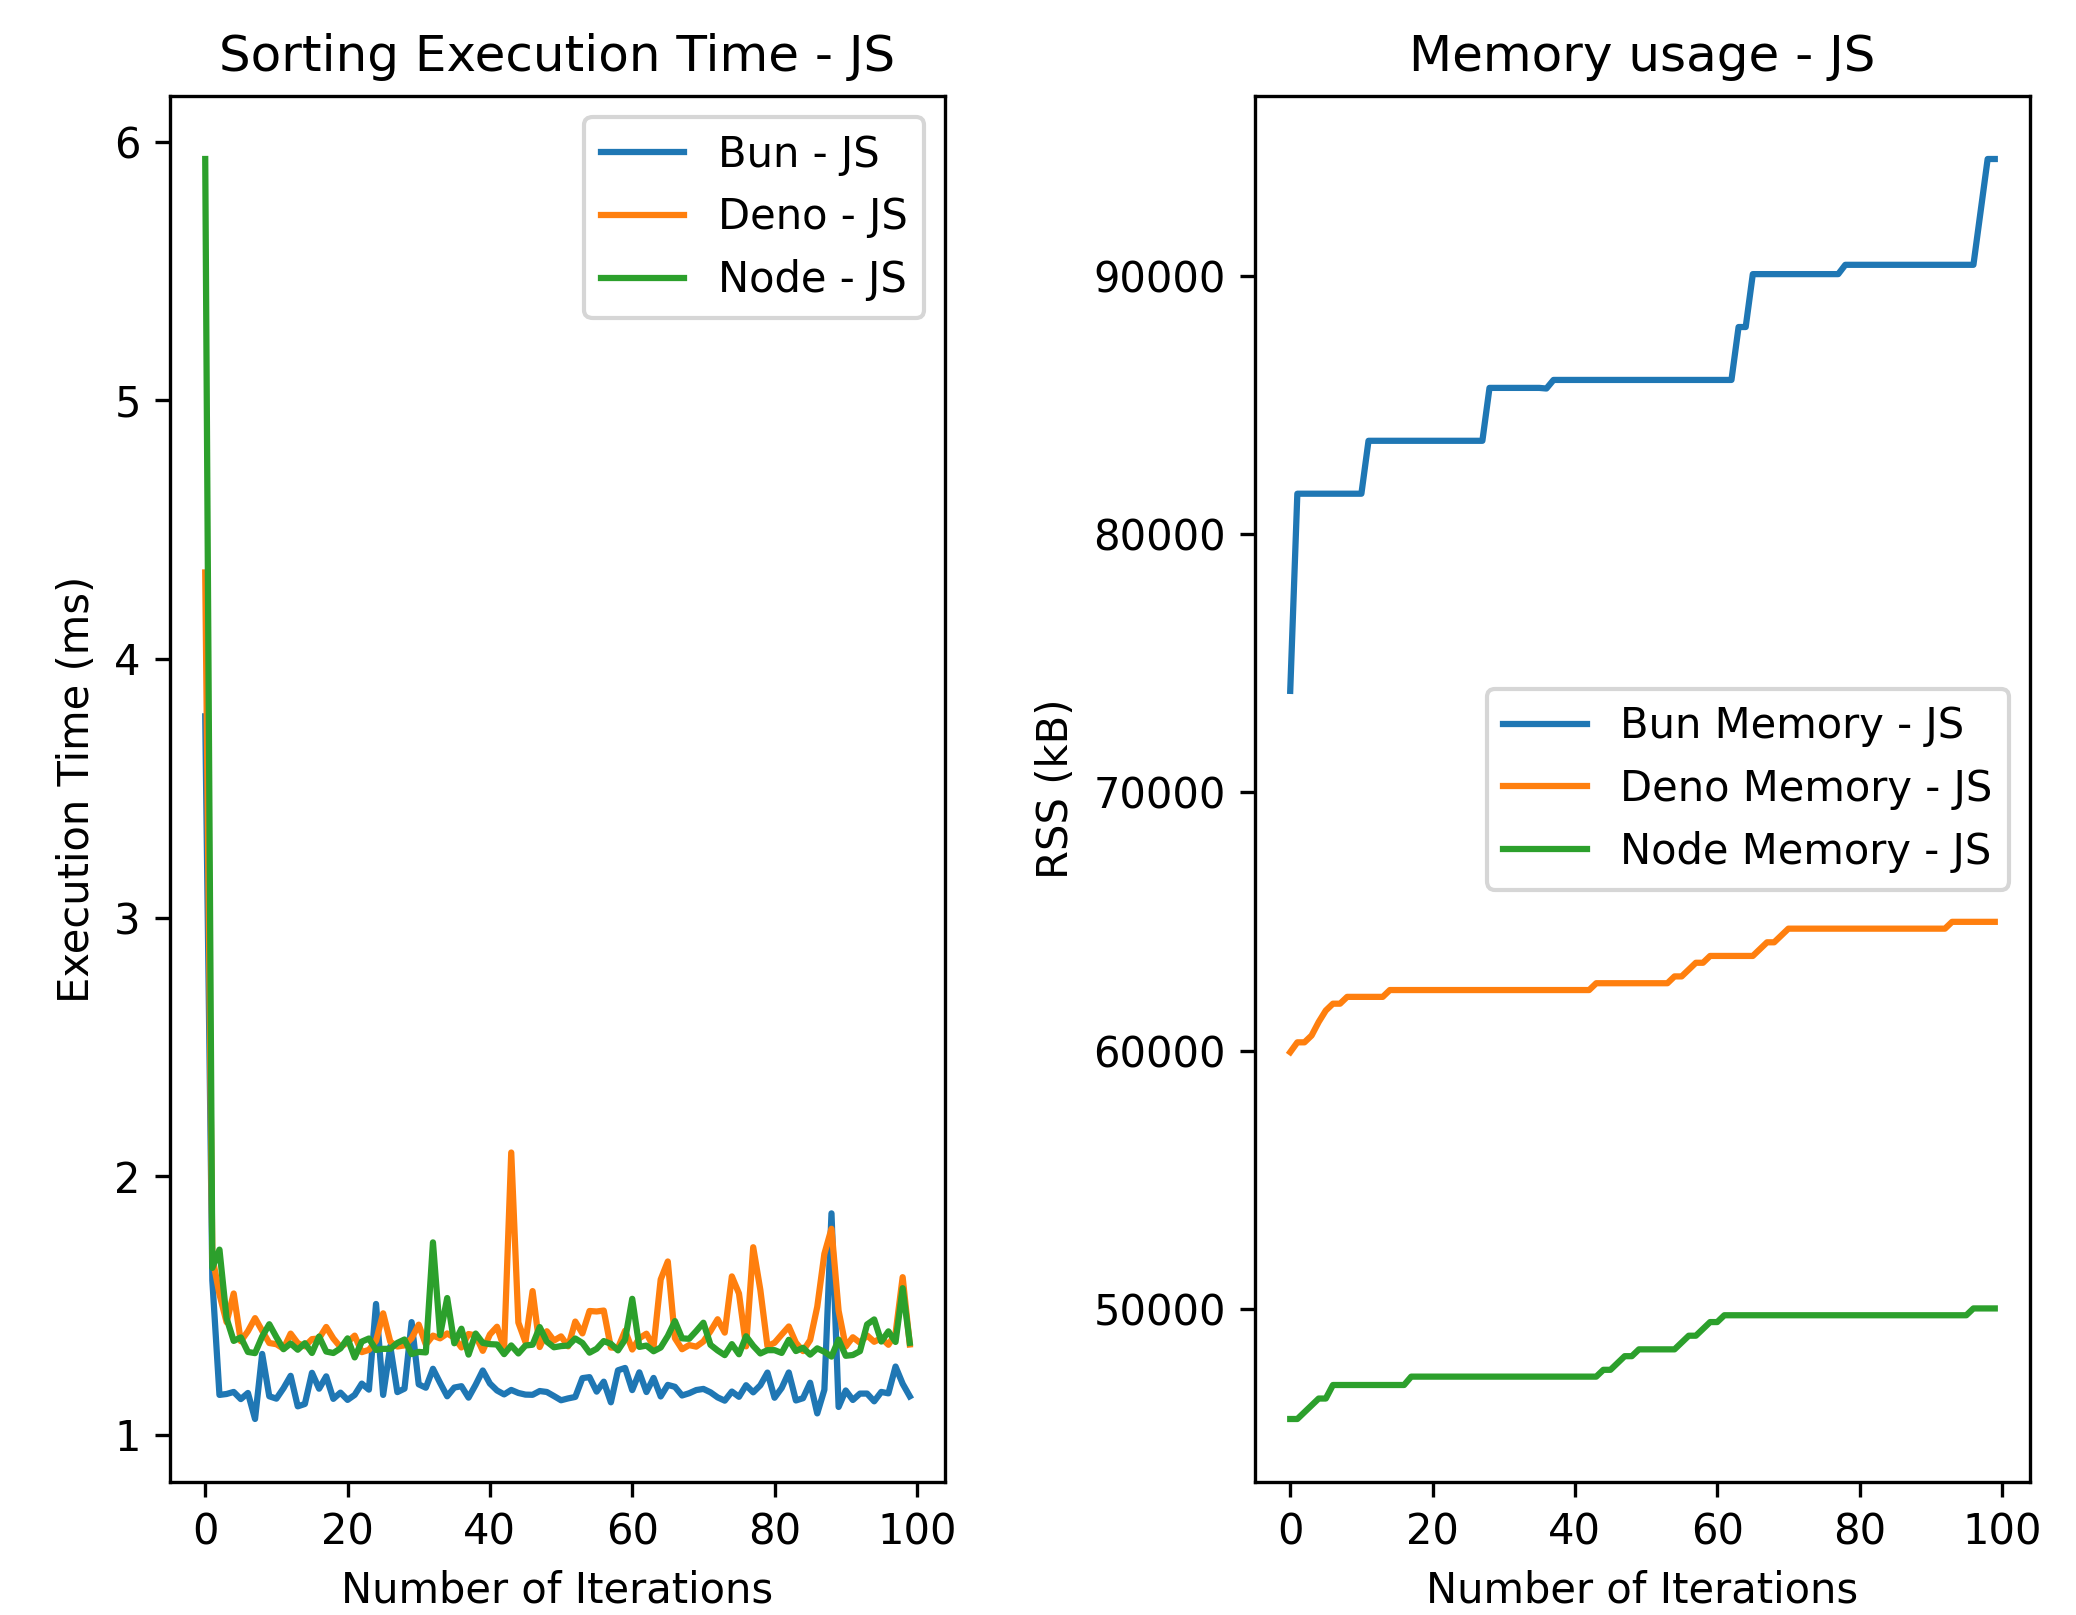
\includegraphics[width=0.68\textwidth]{Figures/sorting/sorting_bubble_100_1000_js.png}
  \caption{Wyniki eksperymentów dla algorytmu sortowania bąbelkowego dla 100 iteracji i 1000 elementów - po lewej czas wykonania jednorazowego testu w milisekundach, po prawej ilość zajmowanej pamięci w kilobajtach (kB)}
  \label{fig:bubble_sorting_e1}
\end{figure}

Na rysunku \ref{fig:bubble_sorting_e1_ts} przedstawiono wyniki eksperymentów dla algorytmu sortowania bąbelkowego dla 100 iteracji i 1000 elementów napisanego w języku TypeScript. Na wykresie przedstawiono czas wykonania jednorazowego testu w milisekundach oraz ilość zajmowanej pamięci w kilobajtach (kB).

\begin{figure}[H]
  \centering
  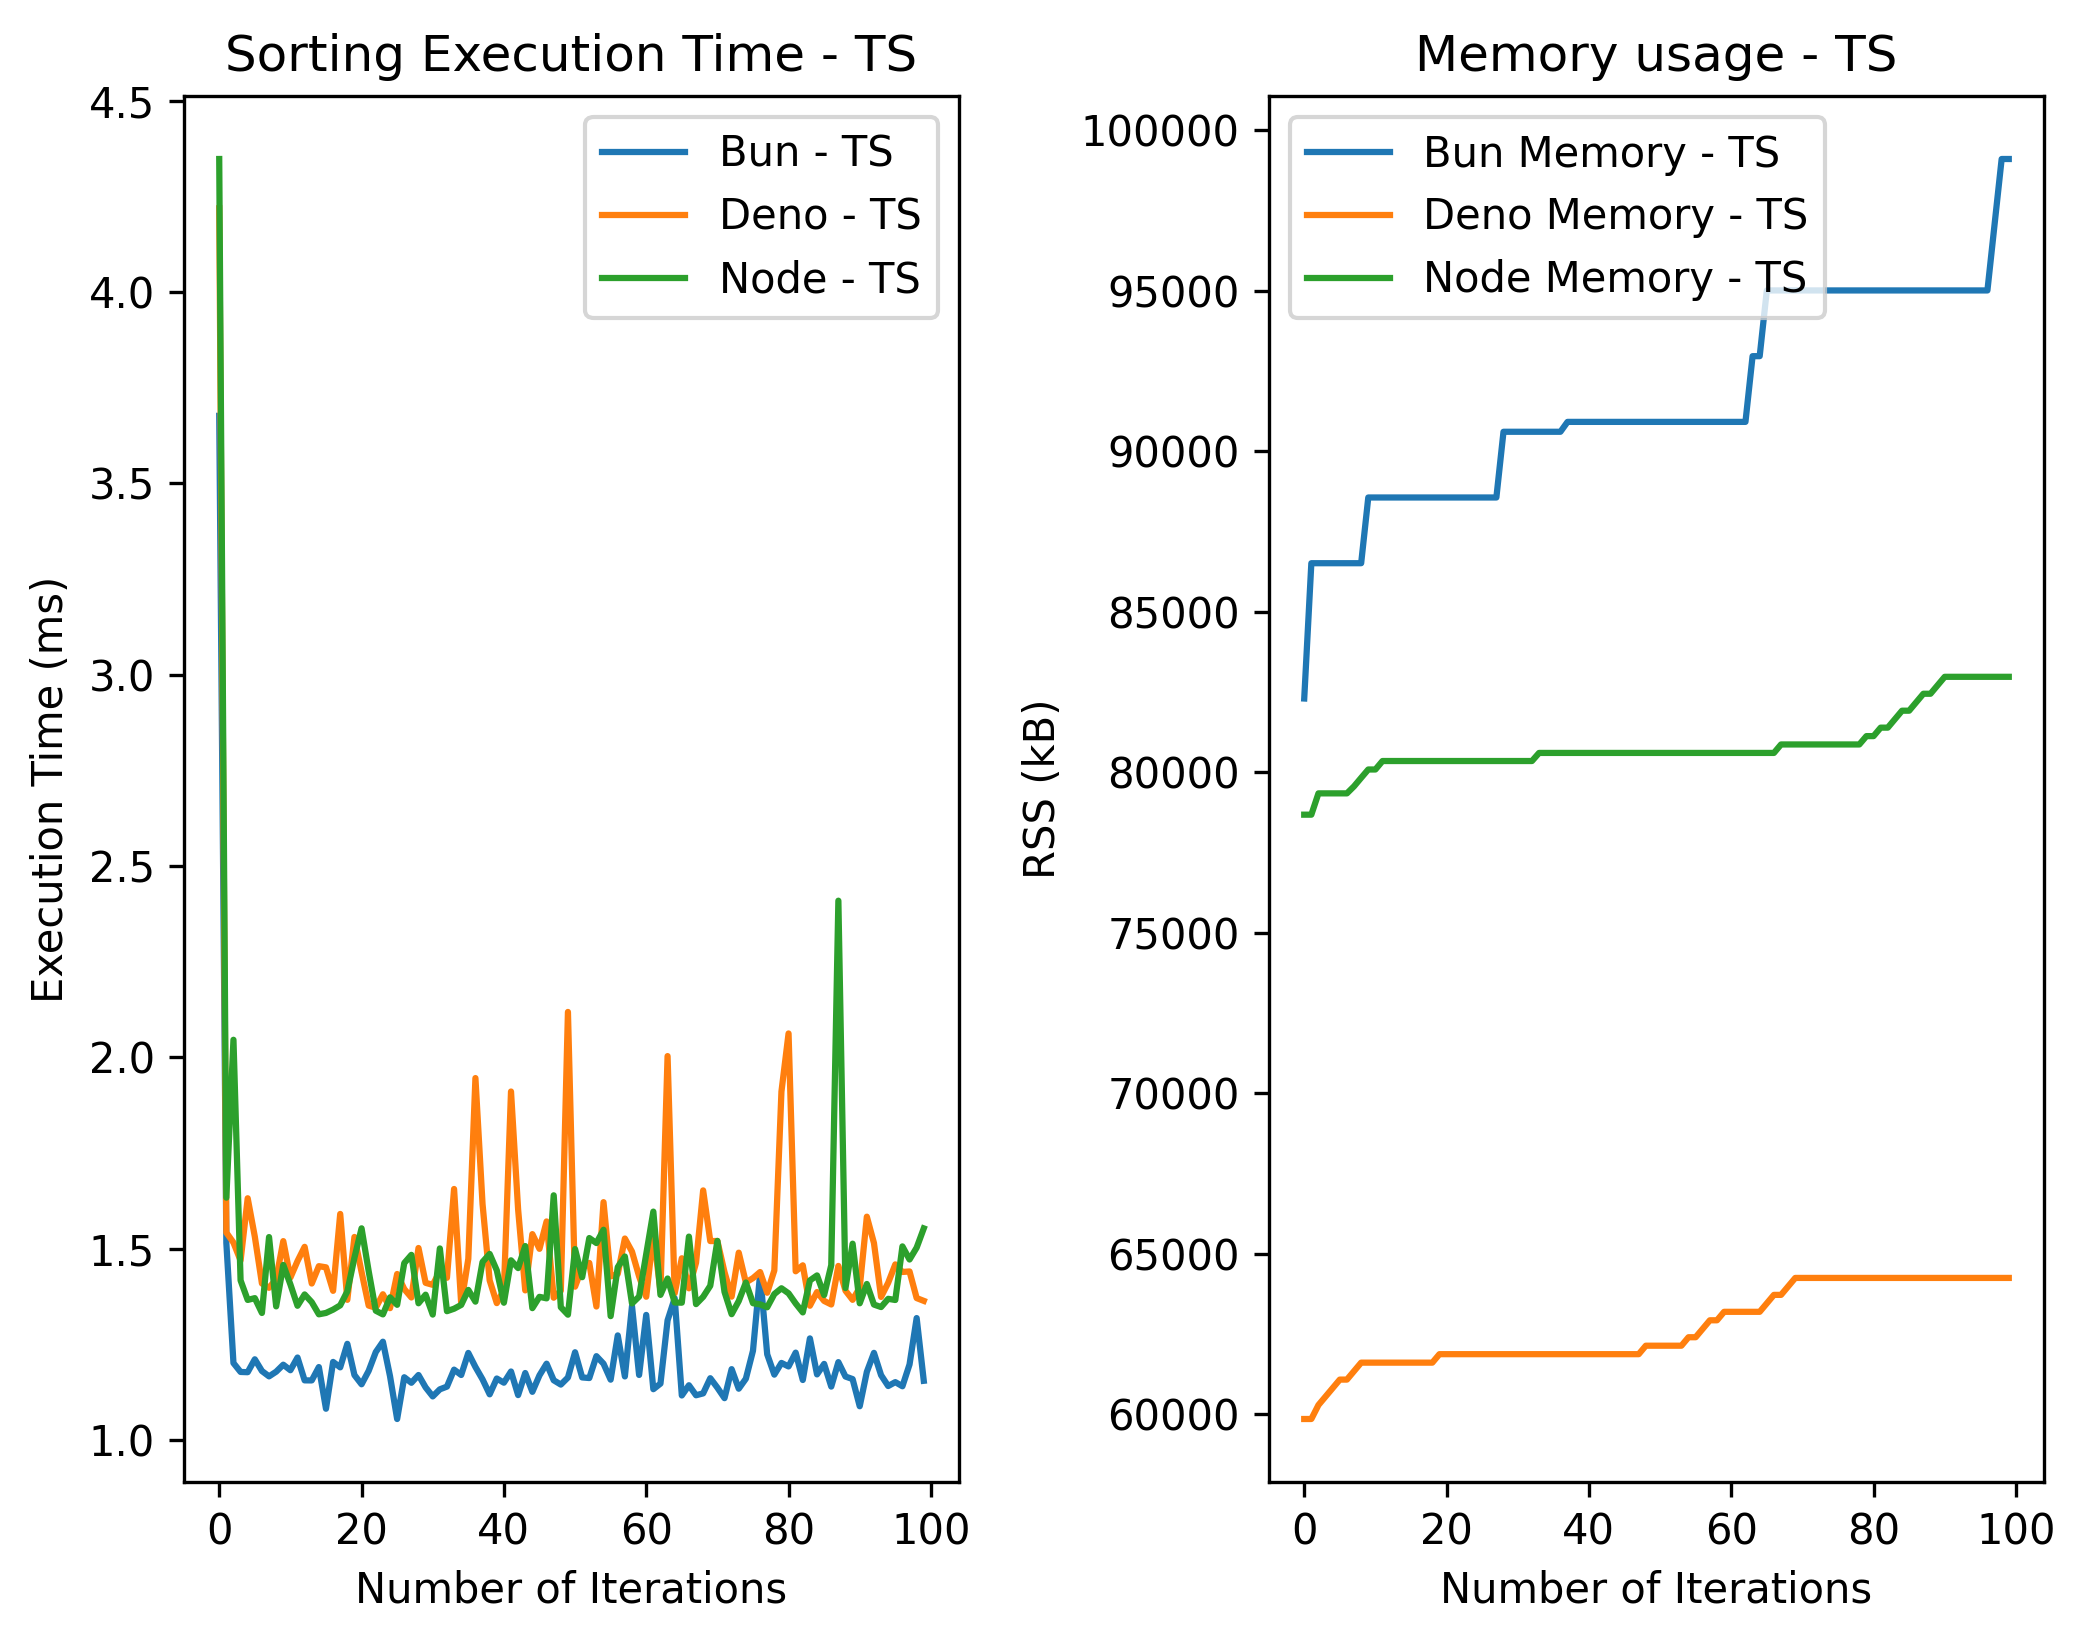
\includegraphics[width=0.68\textwidth]{Figures/sorting/sorting_bubble_100_1000_ts.png}
  \caption{Wyniki eksperymentów dla algorytmu sortowania bąbelkowego dla 100 iteracji i 1000 elementów - po lewej czas wykonania jednorazowego testu w milisekundach, po prawej ilość zajmowanej pamięci w kilobajtach (kB)}
  \label{fig:bubble_sorting_e1_ts}
\end{figure}

Na rysunku \ref{fig:bubble_sorting_e2} przedstawiono wyniki eksperymentów dla algorytmu sortowania bąbelkowego dla 100 iteracji i 1000 elementów napisanego w języku JavaScript. Na wykresie przedstawiono czas wykonania jednorazowego testu w milisekundach oraz ilość zajmowanej pamięci w kilobajtach (kB).

\begin{figure}[H]
  \centering
  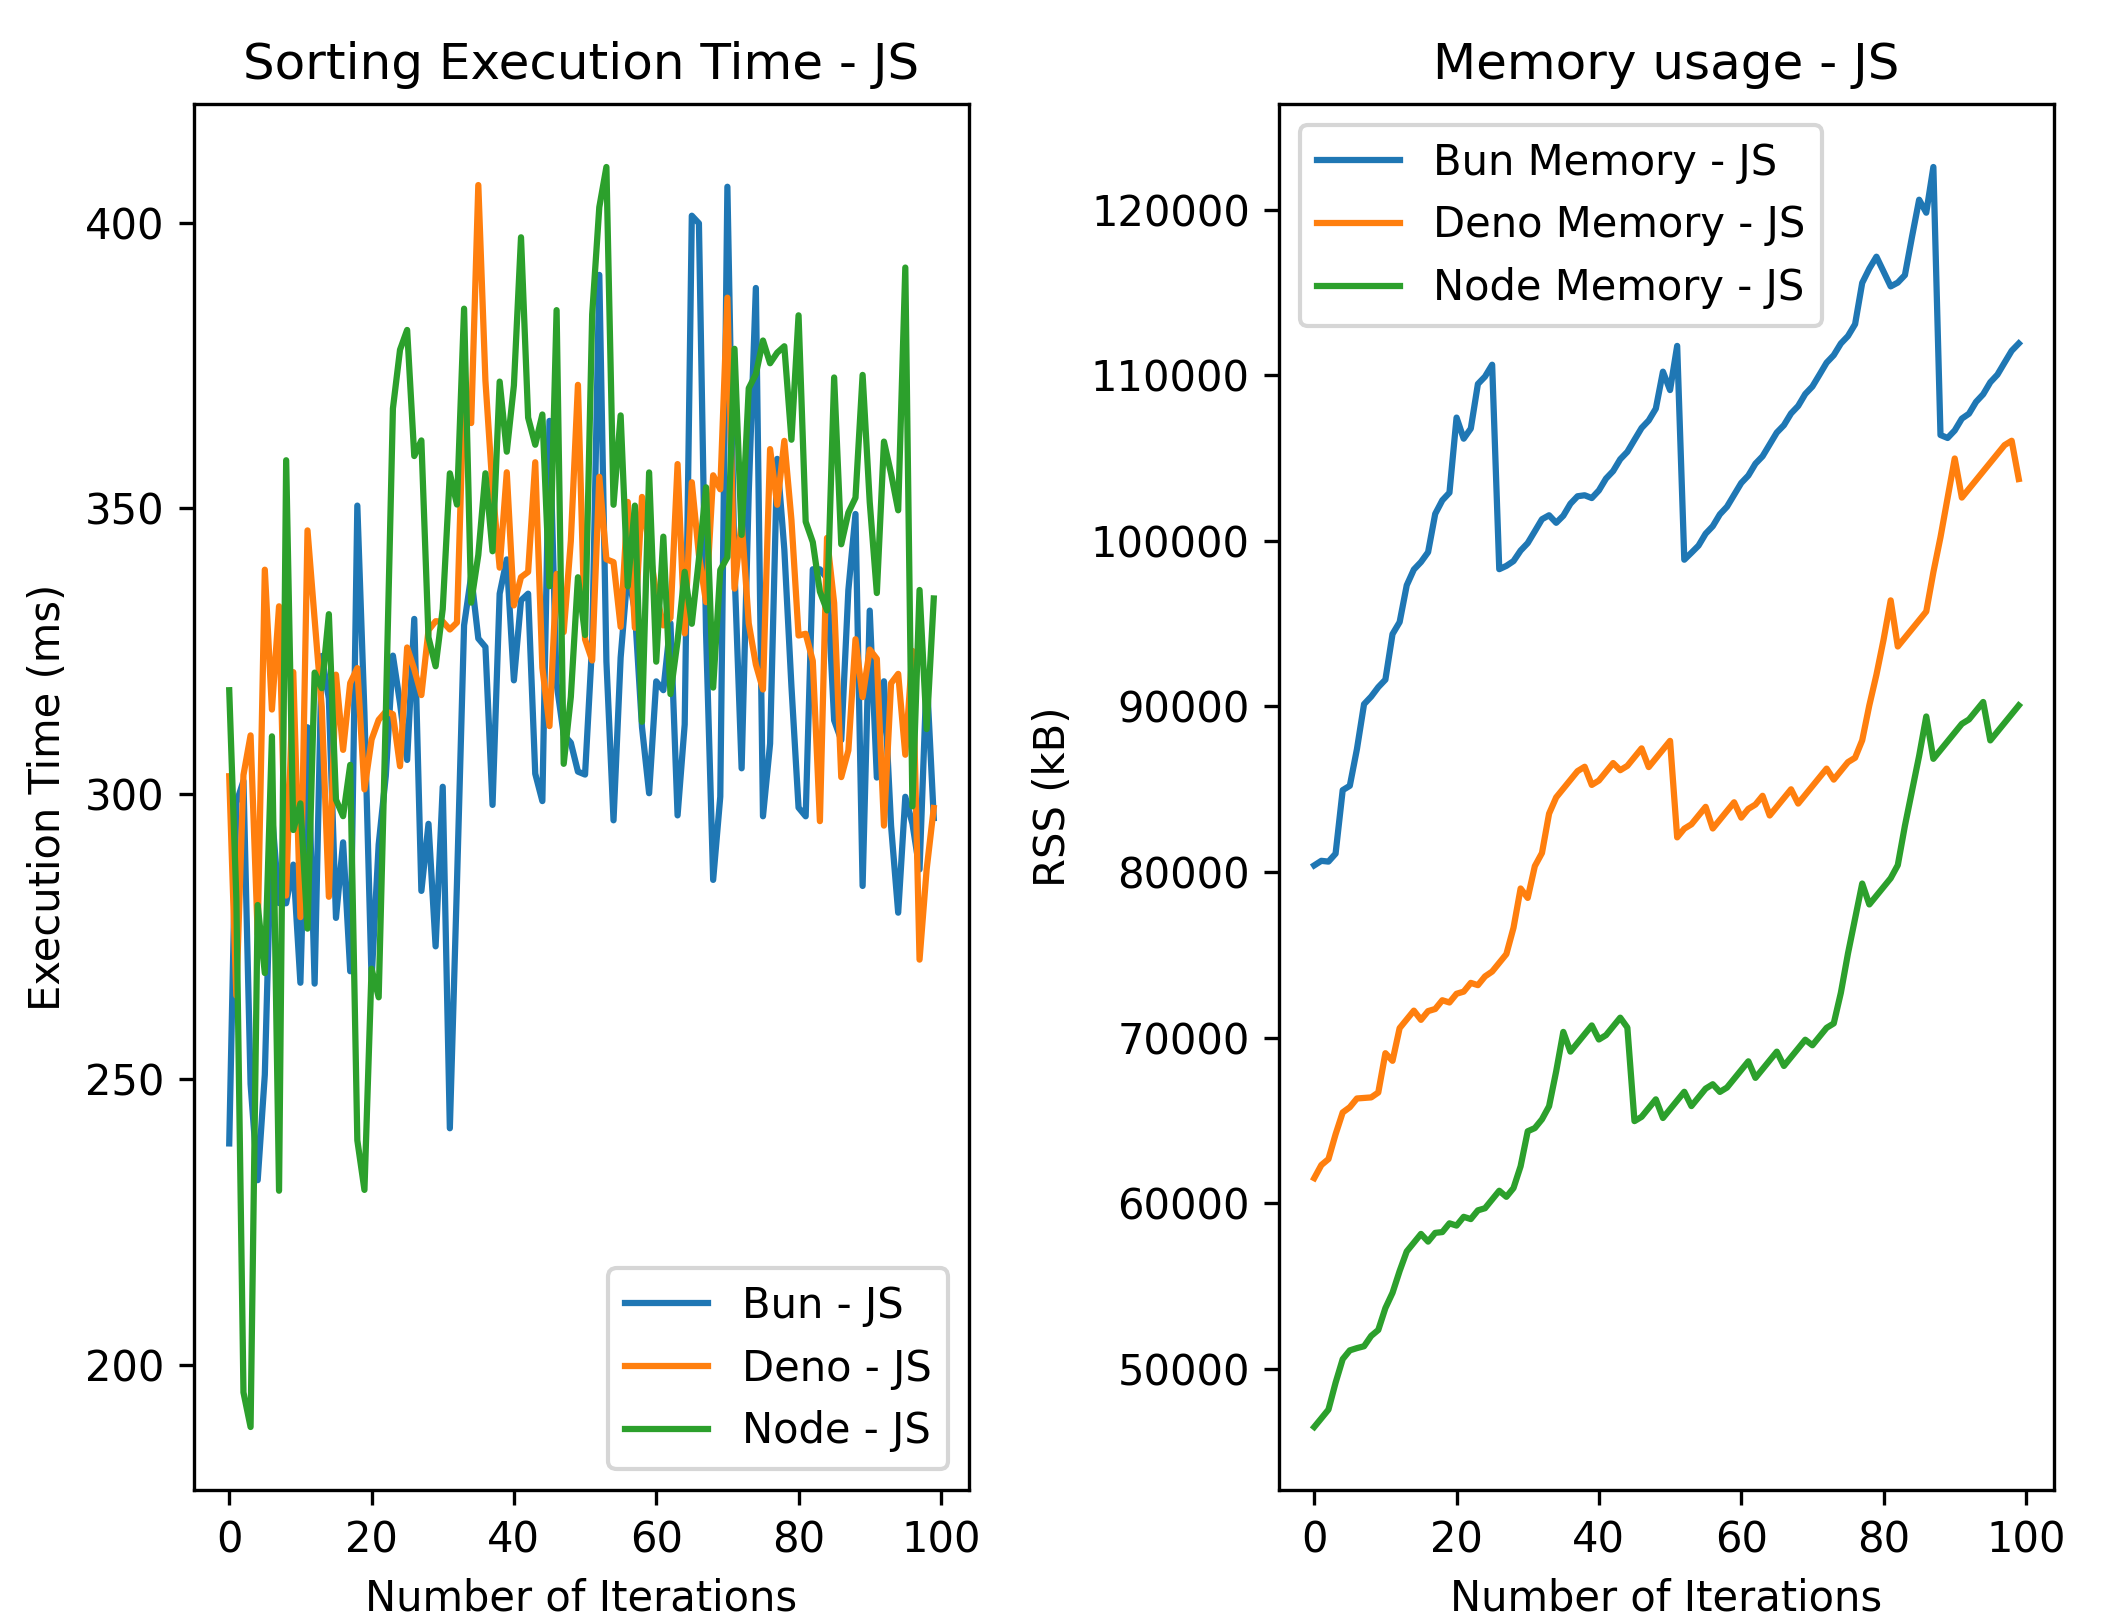
\includegraphics[width=0.68\textwidth]{Figures/sorting/sorting_bubble_100_10000_js.png}
  \caption{Wyniki eksperymentów dla algorytmu sortowania bąbelkowego dla 100 iteracji i 10000 elementów - po lewej czas wykonania jednorazowego testu w milisekundach, po prawej ilość zajmowanej pamięci w kilobajtach (kB)}
  \label{fig:bubble_sorting_e2}
\end{figure}

Na rysunku \ref{fig:bubble_sorting_e2_ts} przedstawiono wyniki eksperymentów dla algorytmu sortowania bąbelkowego dla 100 iteracji i 10000 elementów napisanego w języku TypeScript. Na wykresie przedstawiono czas wykonania jednorazowego testu w milisekundach oraz ilość zajmowanej pamięci w kilobajtach (kB).

\begin{figure}[H]
  \centering
  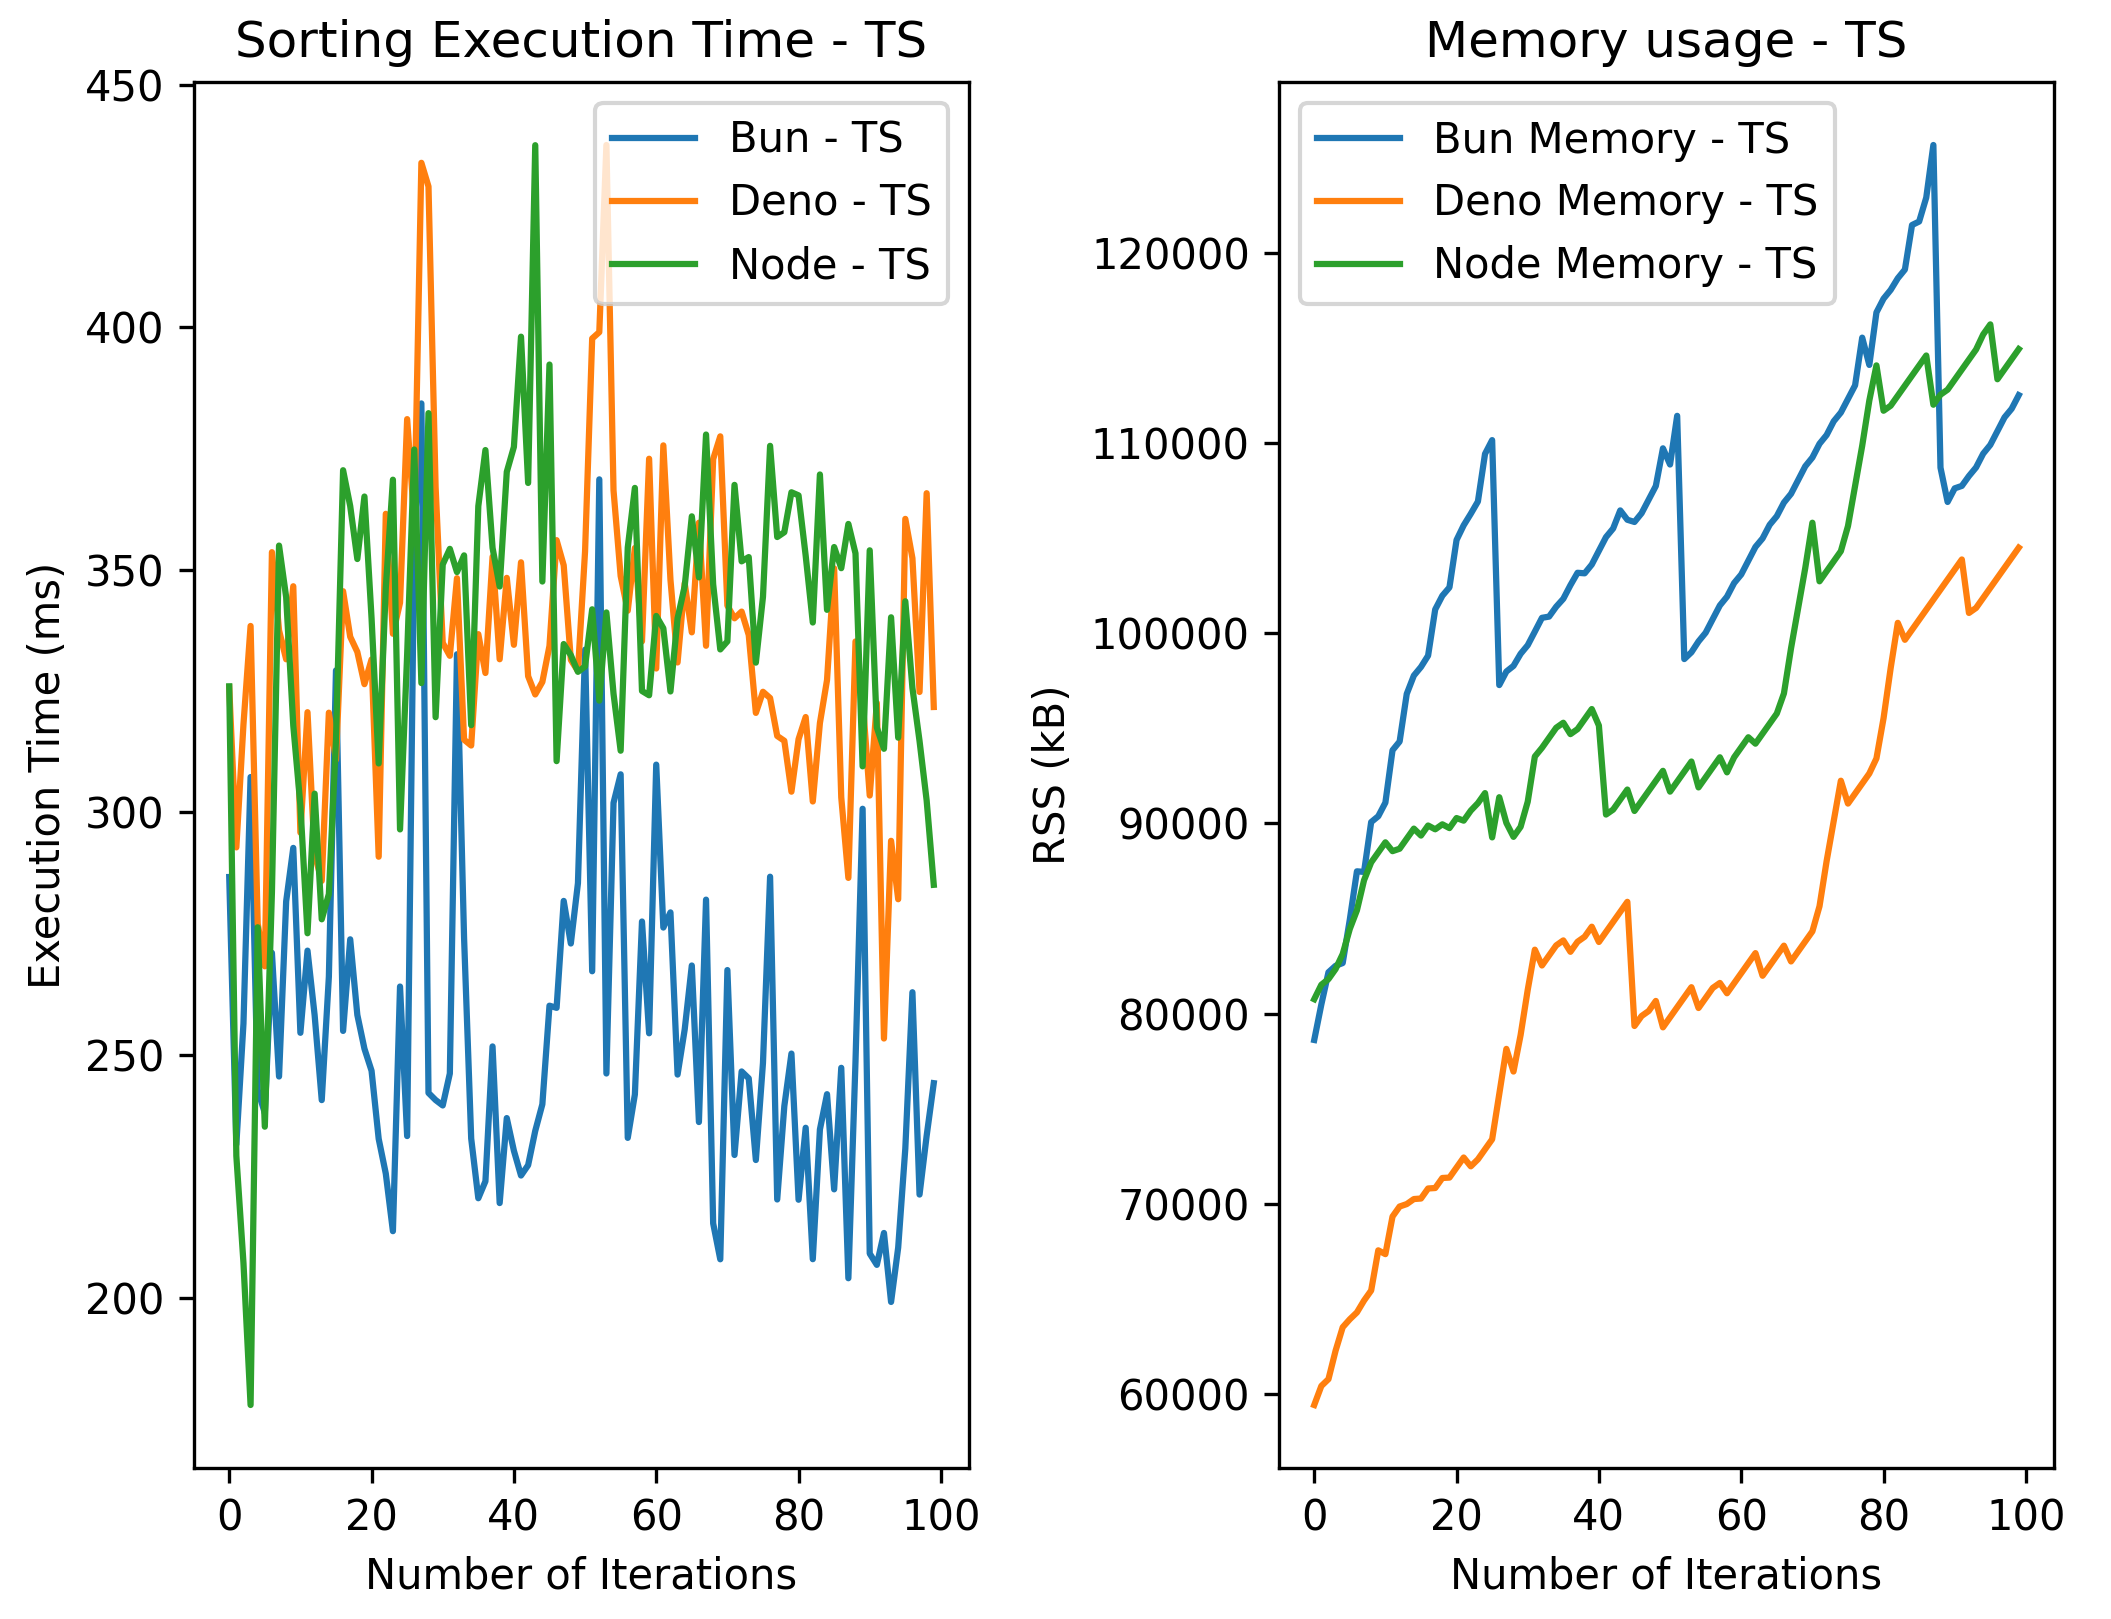
\includegraphics[width=0.68\textwidth]{Figures/sorting/sorting_bubble_100_10000_ts.png}
  \caption{Wyniki eksperymentów dla algorytmu sortowania bąbelkowego dla 100 iteracji i 10000 elementów - po lewej czas wykonania jednorazowego testu w milisekundach, po prawej ilość zajmowanej pamięci w kilobajtach (kB)}
  \label{fig:bubble_sorting_e2_ts}
\end{figure}

Na rysunku \ref{fig:bubble_sorting_e3} przedstawiono wyniki eksperymentów dla algorytmu sortowania bąbelkowego dla 1000 iteracji i 1000 elementów napisanego w języku JavaScript. Na wykresie przedstawiono czas wykonania jednorazowego testu w milisekundach oraz ilość zajmowanej pamięci w kilobajtach (kB).

\begin{figure}[H]
  \centering
  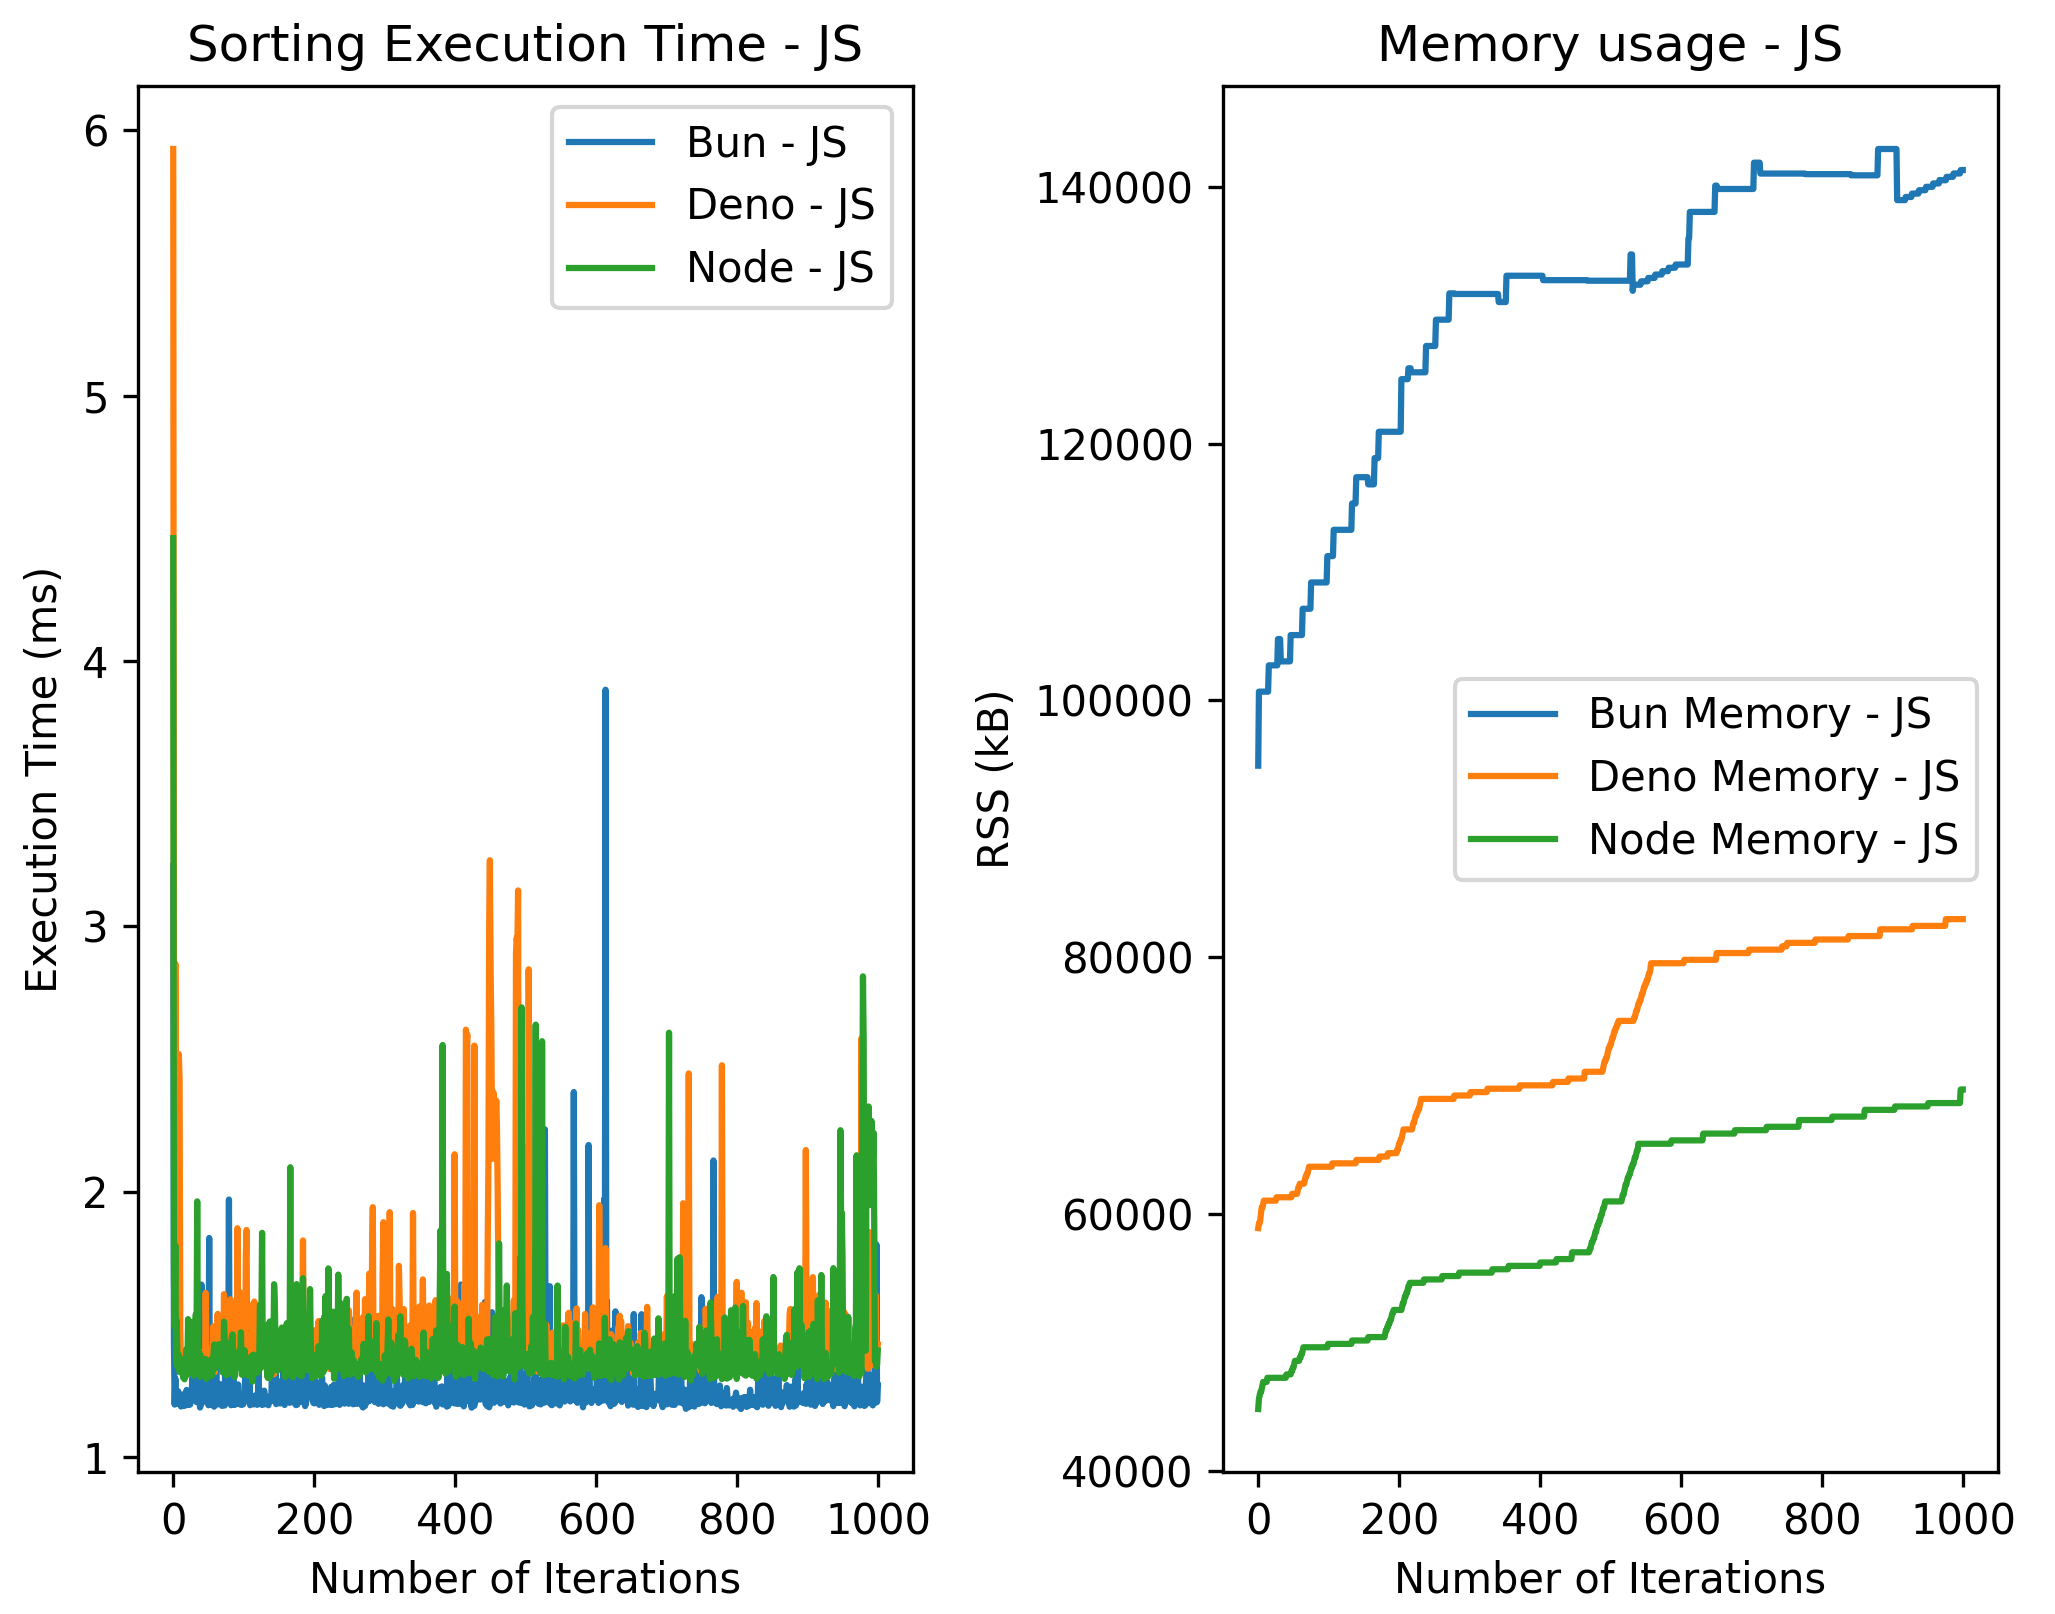
\includegraphics[width=0.68\textwidth]{Figures/sorting/sorting_bubble_1000_1000_js.png}
  \caption{Wyniki eksperymentów dla algorytmu sortowania bąbelkowego dla 1000 iteracji i 1000 elementów - po lewej czas wykonania jednorazowego testu w milisekundach, po prawej ilość zajmowanej pamięci w kilobajtach (kB)}
  \label{fig:bubble_sorting_e3}
\end{figure}

Na rysunku \ref{fig:bubble_sorting_e3_ts} przedstawiono wyniki eksperymentów dla algorytmu sortowania bąbelkowego dla 1000 iteracji i 1000 elementów napisanego w języku TypeScript. Na wykresie przedstawiono czas wykonania jednorazowego testu w milisekundach oraz ilość zajmowanej pamięci w kilobajtach (kB).

\begin{figure}[H]
  \centering
  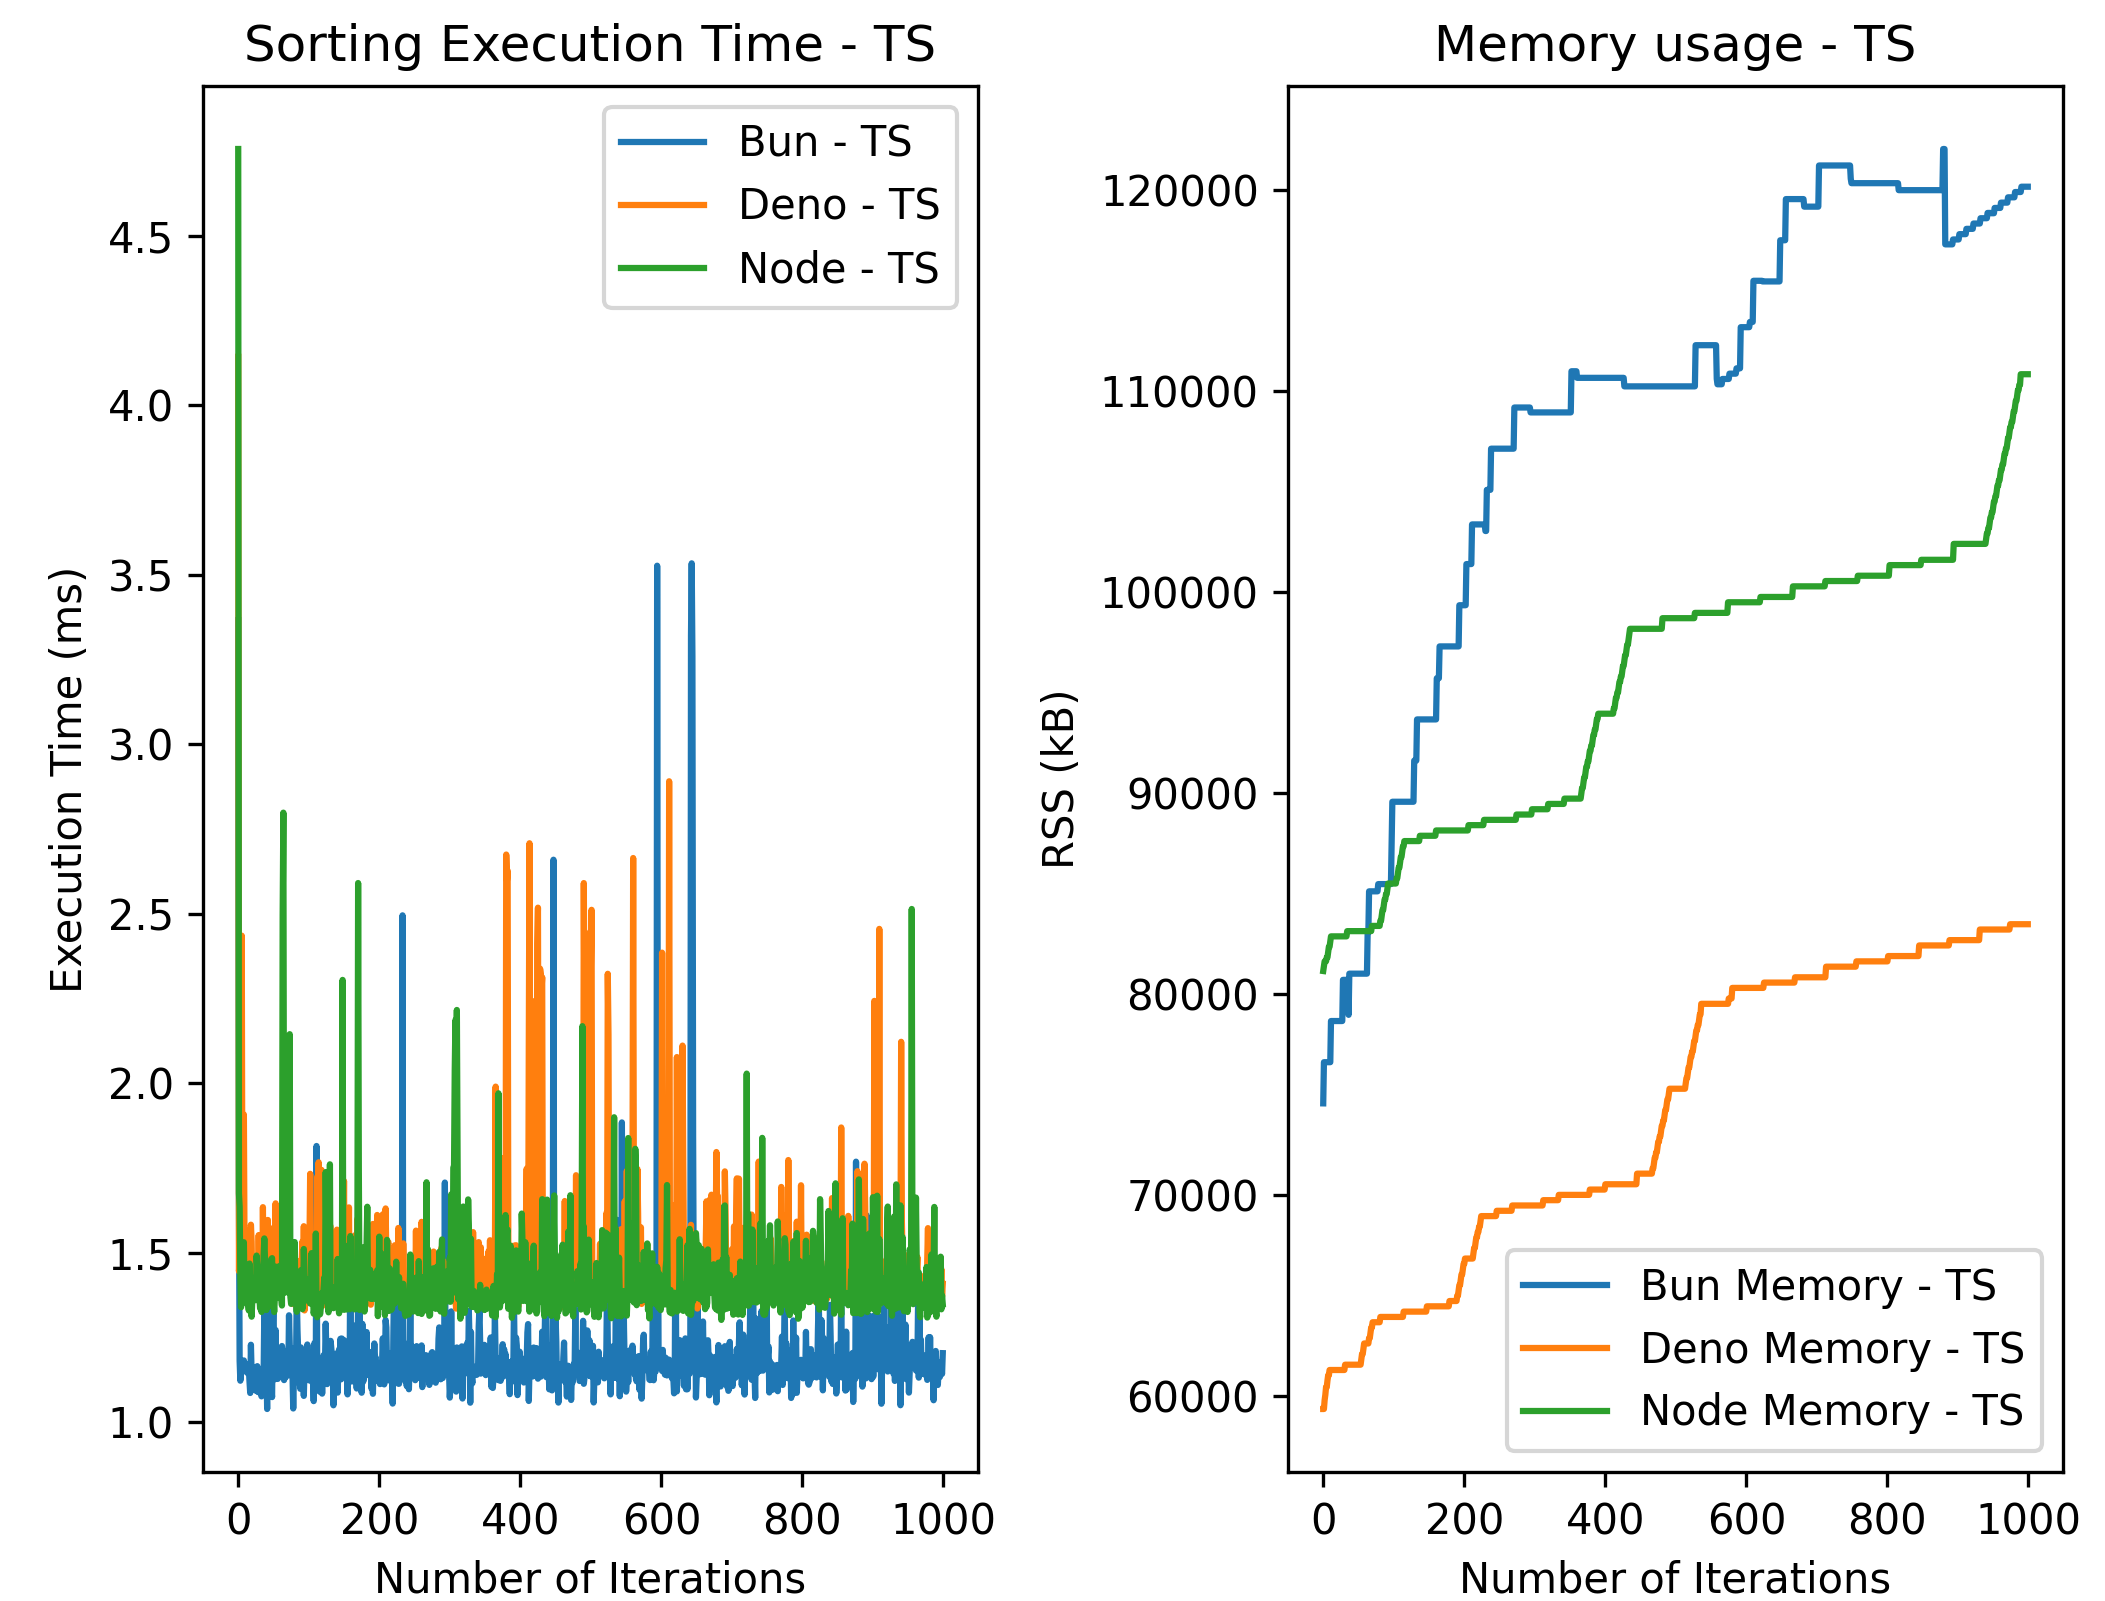
\includegraphics[width=0.68\textwidth]{Figures/sorting/sorting_bubble_1000_1000_ts.png}
  \caption{Wyniki eksperymentów dla algorytmu sortowania bąbelkowego dla 100 iteracji i 1000 elementów - po lewej czas wykonania jednorazowego testu w milisekundach, po prawej ilość zajmowanej pamięci w kilobajtach (kB)}
  \label{fig:bubble_sorting_e3_ts}
\end{figure}

Na rysunku \ref{fig:bubble_sorting_e4} przedstawiono wyniki eksperymentów dla algorytmu sortowania bąbelkowego dla 100 iteracji i 1000 elementów napisanego w języku JavaScript. Na wykresie przedstawiono czas wykonania jednorazowego testu w milisekundach oraz ilość zajmowanej pamięci w kilobajtach (kB).

\begin{figure}[H]
  \centering
  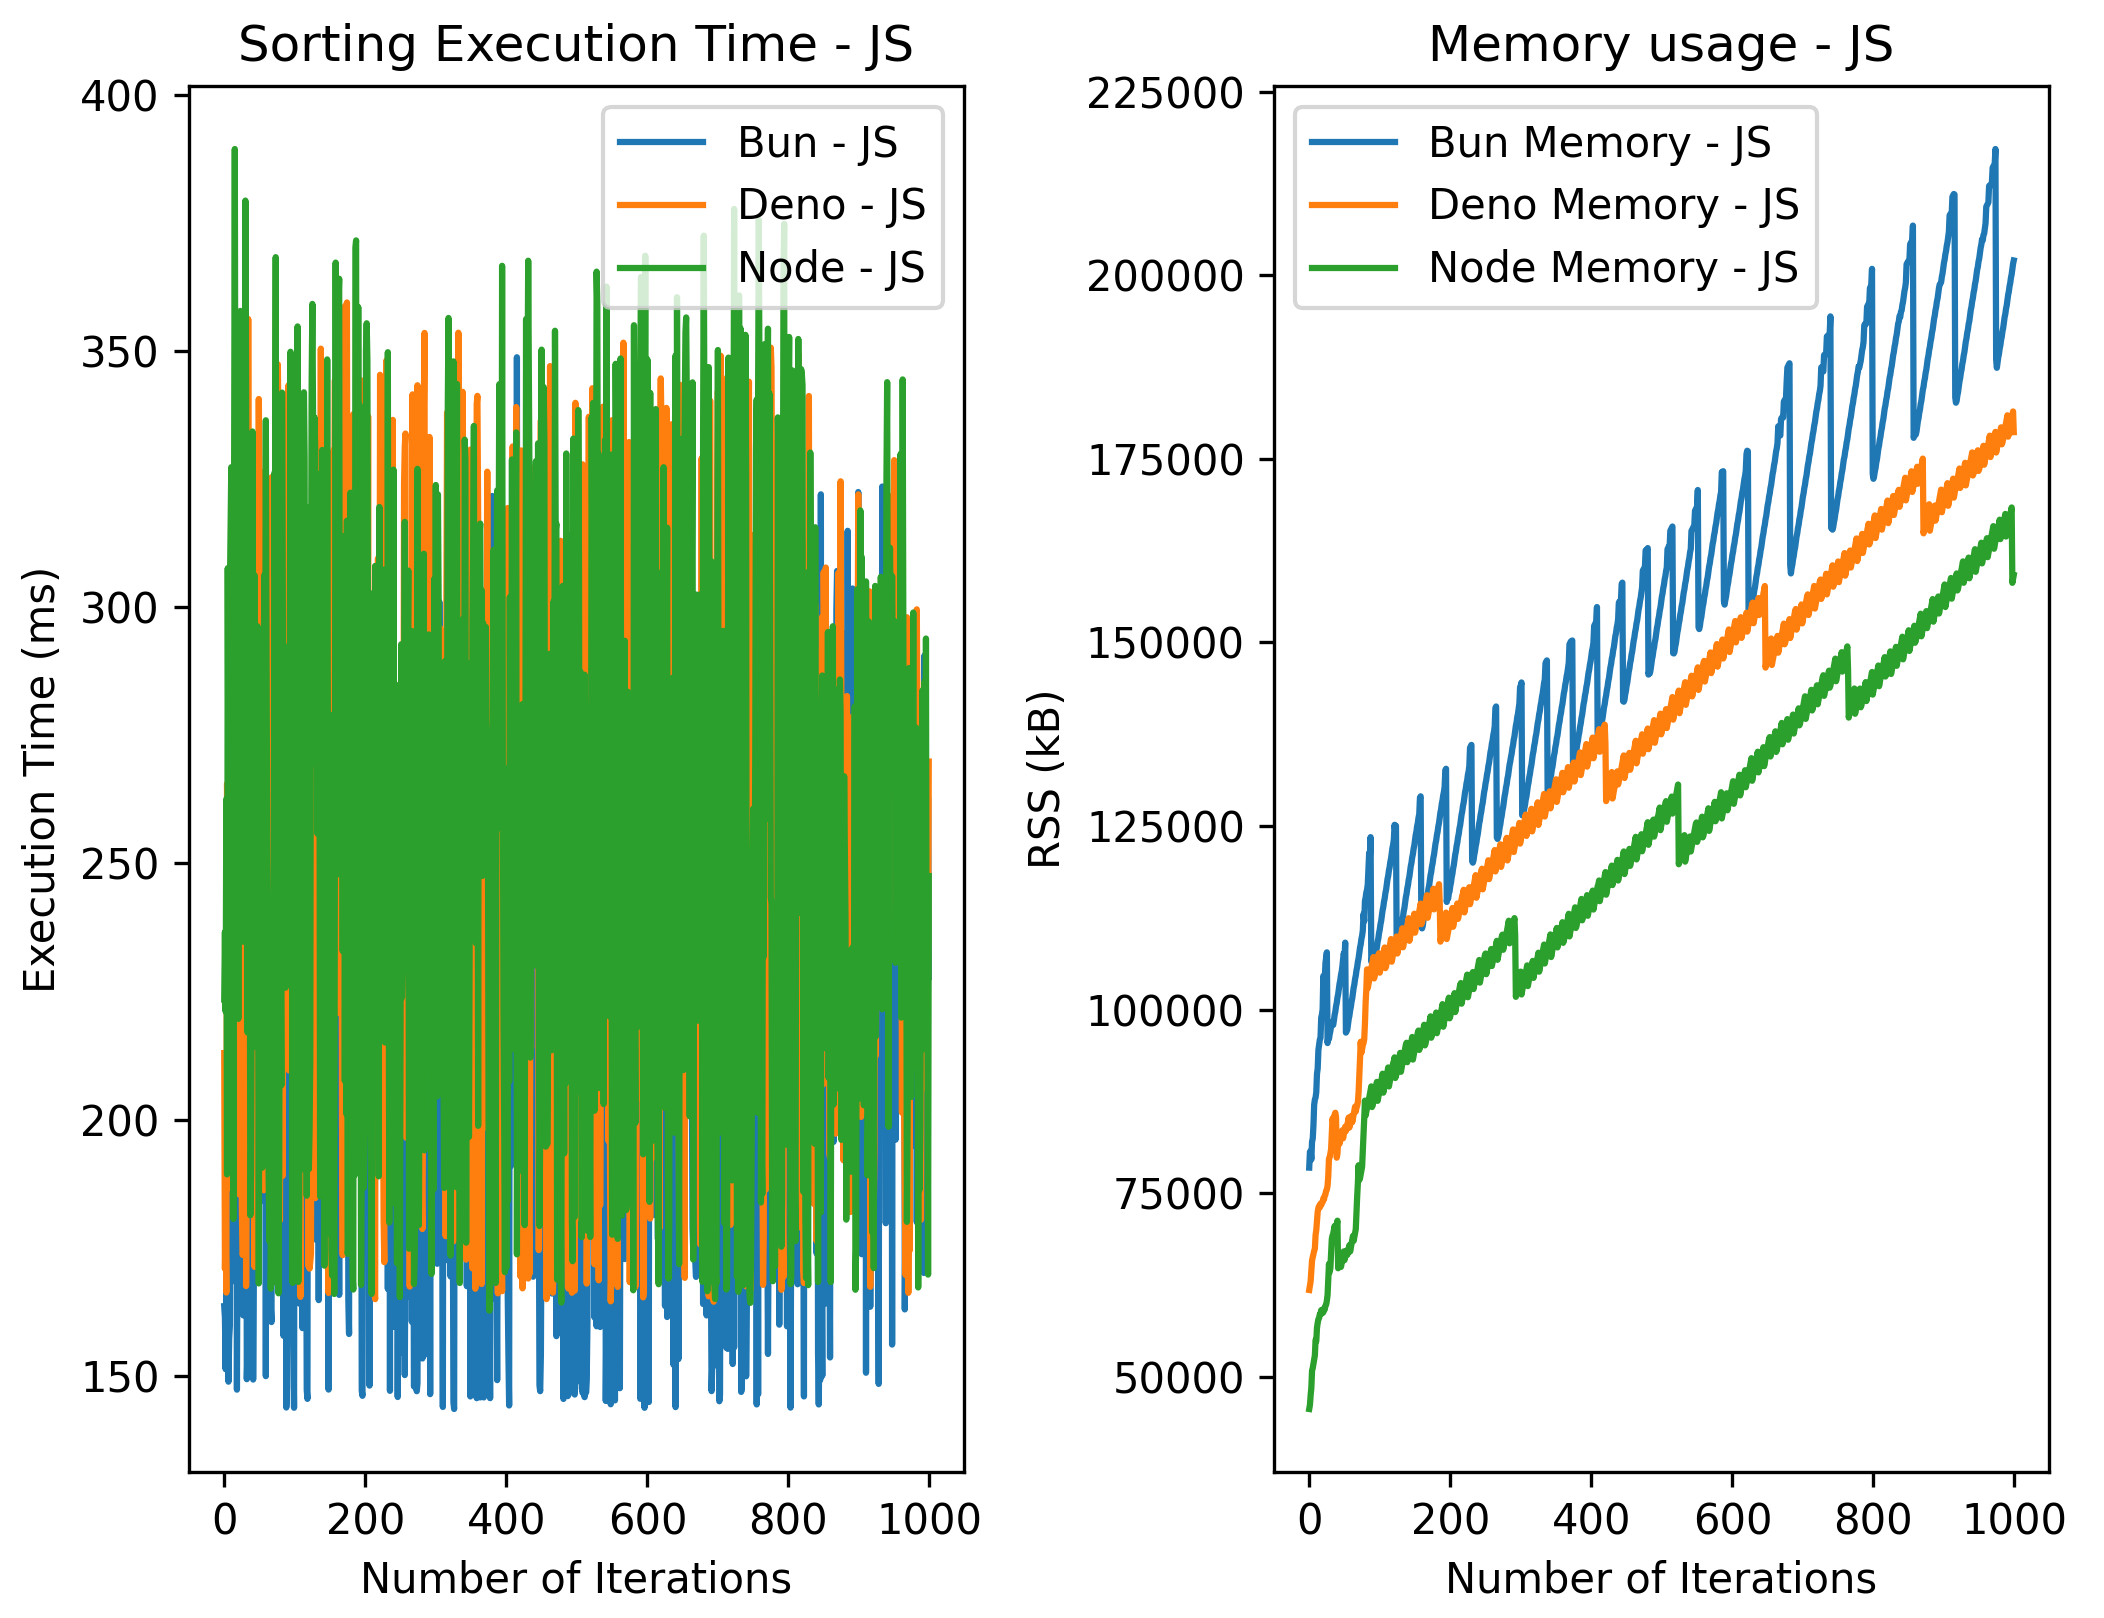
\includegraphics[width=0.68\textwidth]{Figures/sorting/sorting_bubble_1000_10000_js.png}
  \caption{Wyniki eksperymentów dla algorytmu sortowania bąbelkowego dla 100 iteracji i 10000 elementów - po lewej czas wykonania jednorazowego testu w milisekundach, po prawej ilość zajmowanej pamięci w kilobajtach (kB)}
  \label{fig:bubble_sorting_e4}
\end{figure}

Na rysunku \ref{fig:bubble_sorting_e4_ts} przedstawiono wyniki eksperymentów dla algorytmu sortowania bąbelkowego dla 100 iteracji i 10000 elementów napisanego w języku TypeScript. Na wykresie przedstawiono czas wykonania jednorazowego testu w milisekundach oraz ilość zajmowanej pamięci w kilobajtach (kB).

\begin{figure}[H]
  \centering
  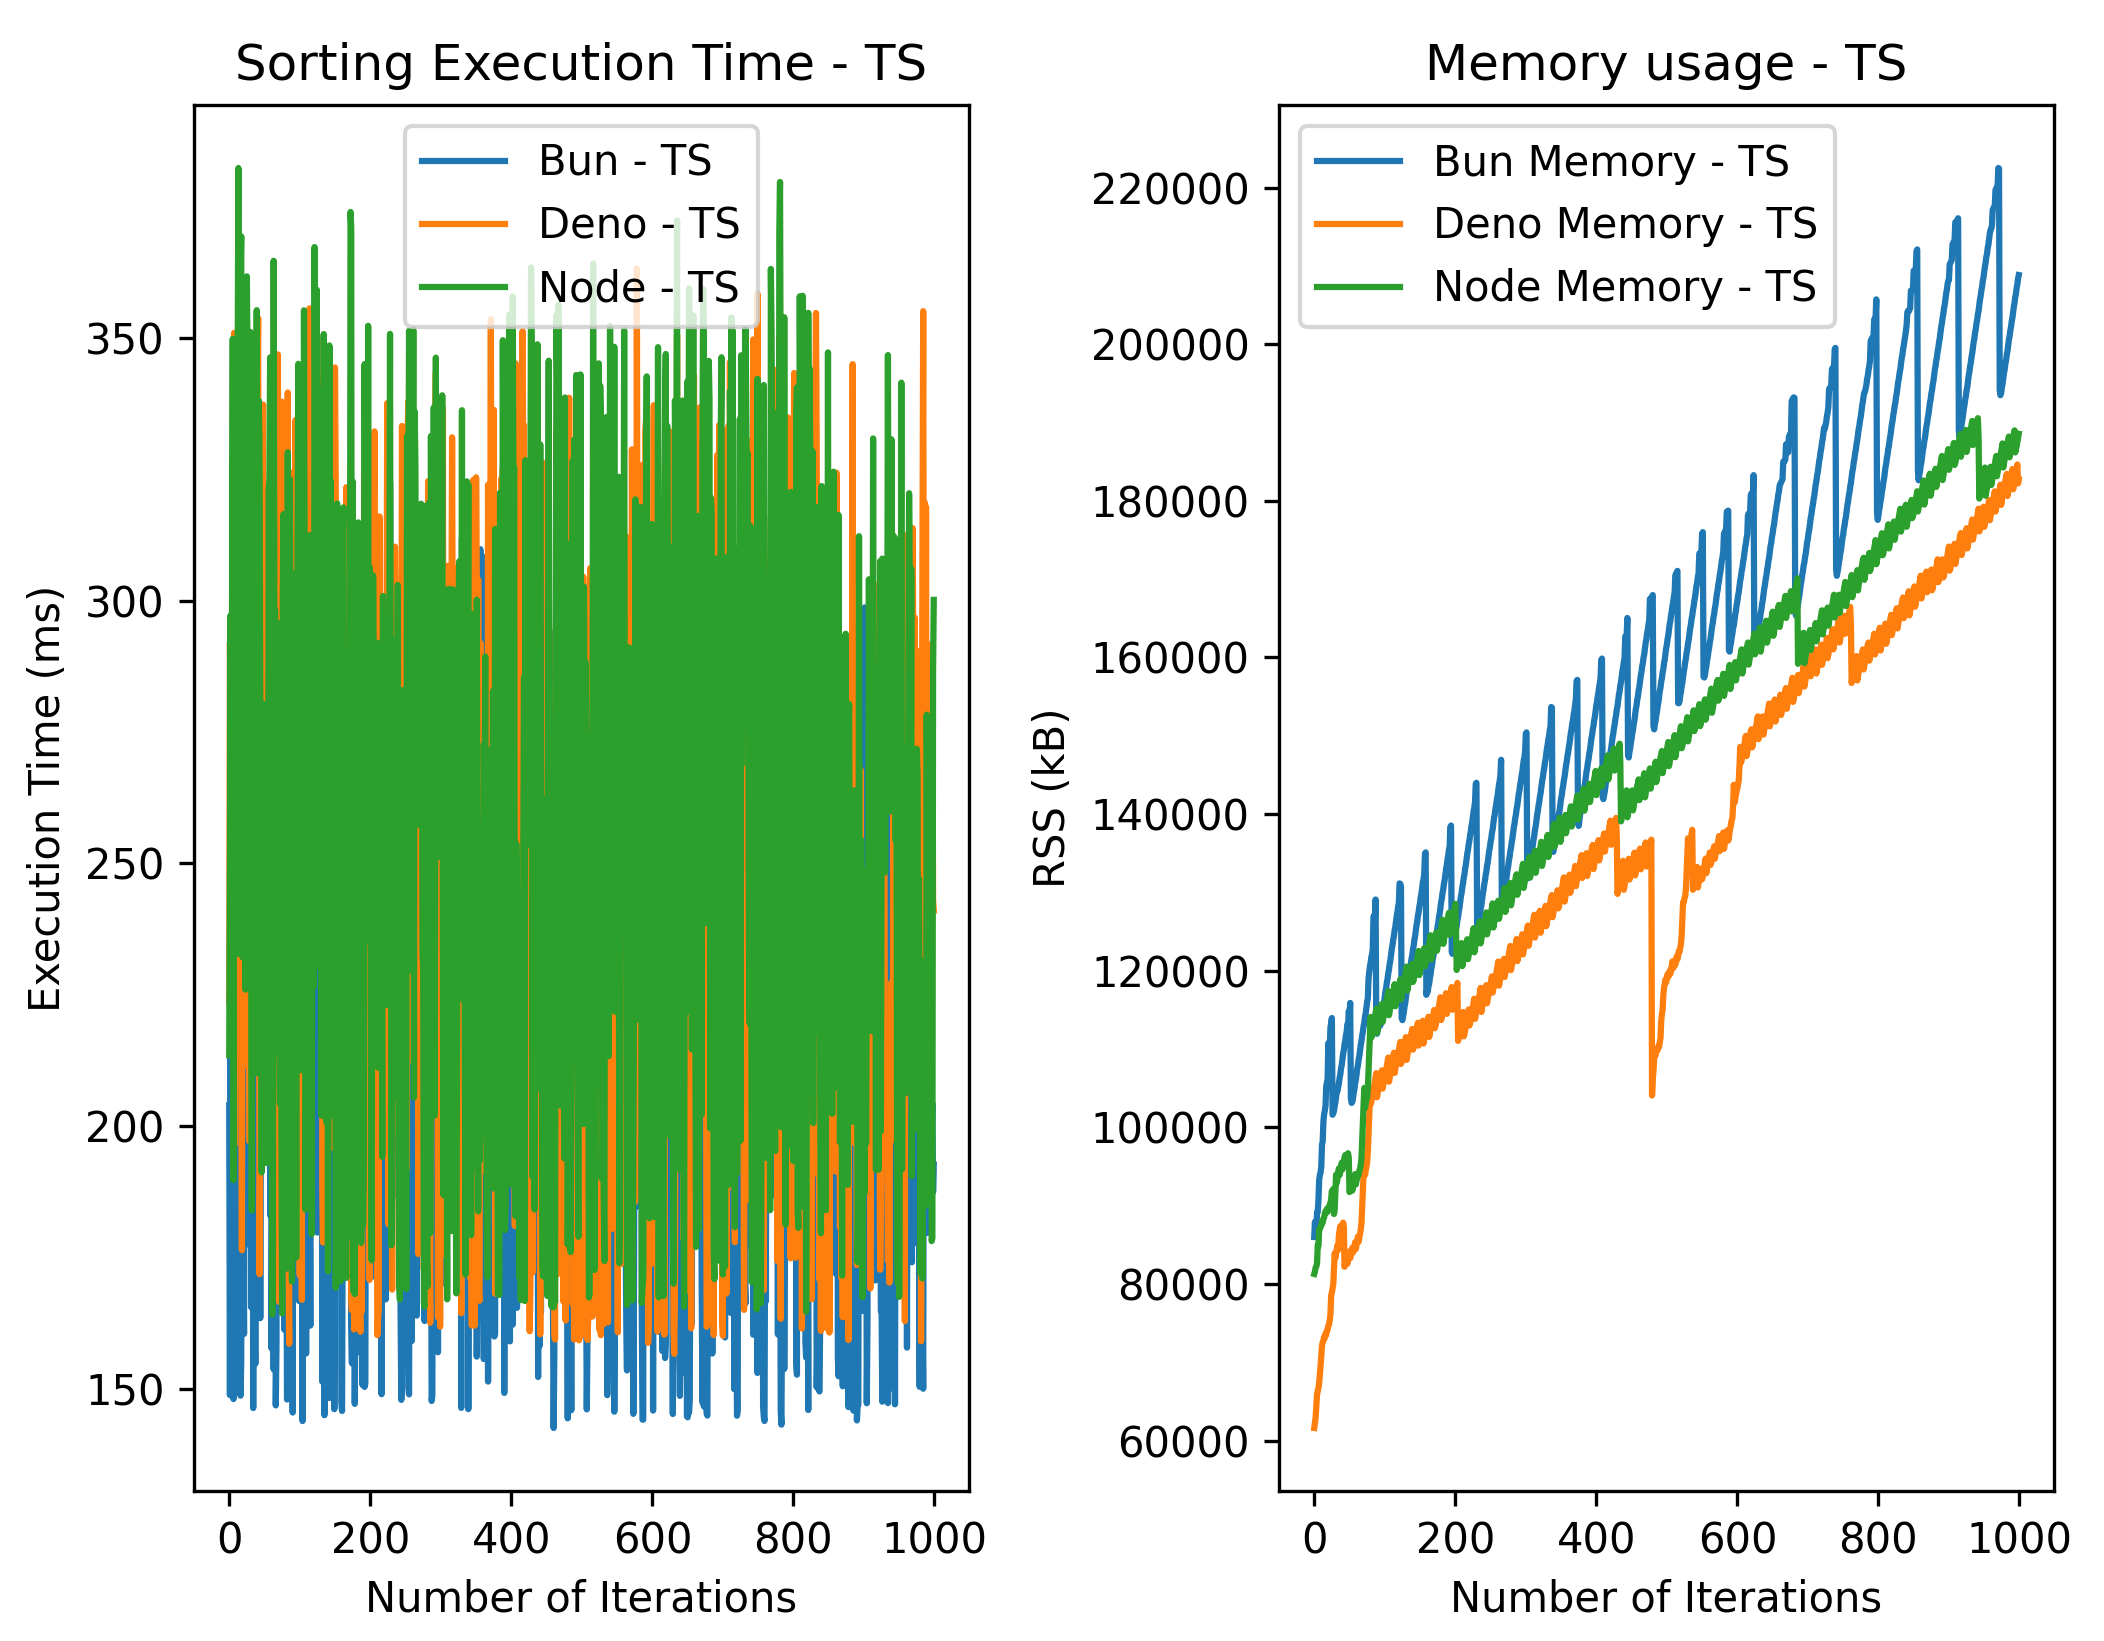
\includegraphics[width=0.68\textwidth]{Figures/sorting/sorting_bubble_1000_10000_ts.png}
  \caption{Wyniki eksperymentów dla algorytmu sortowania bąbelkowego dla 1000 iteracji i 10000 elementów - po lewej czas wykonania jednorazowego testu w milisekundach, po prawej ilość zajmowanej pamięci w kilobajtach (kB)}
  \label{fig:bubble_sorting_e4_ts}
\end{figure}

\subsubsection{Wyniki - sortowanie szybkie}
Na rysunku \ref{fig:quick_sorting_e1} przedstawiono wyniki eksperymentów dla algorytmu sortowania szybkiego dla 100 iteracji i 1000 elementów napisanego w języku JavaScript. Na wykresie przedstawiono czas wykonania jednorazowego testu w milisekundach oraz ilość zajmowanej pamięci w kilobajtach (kB).

\begin{figure}[H]
  \centering
  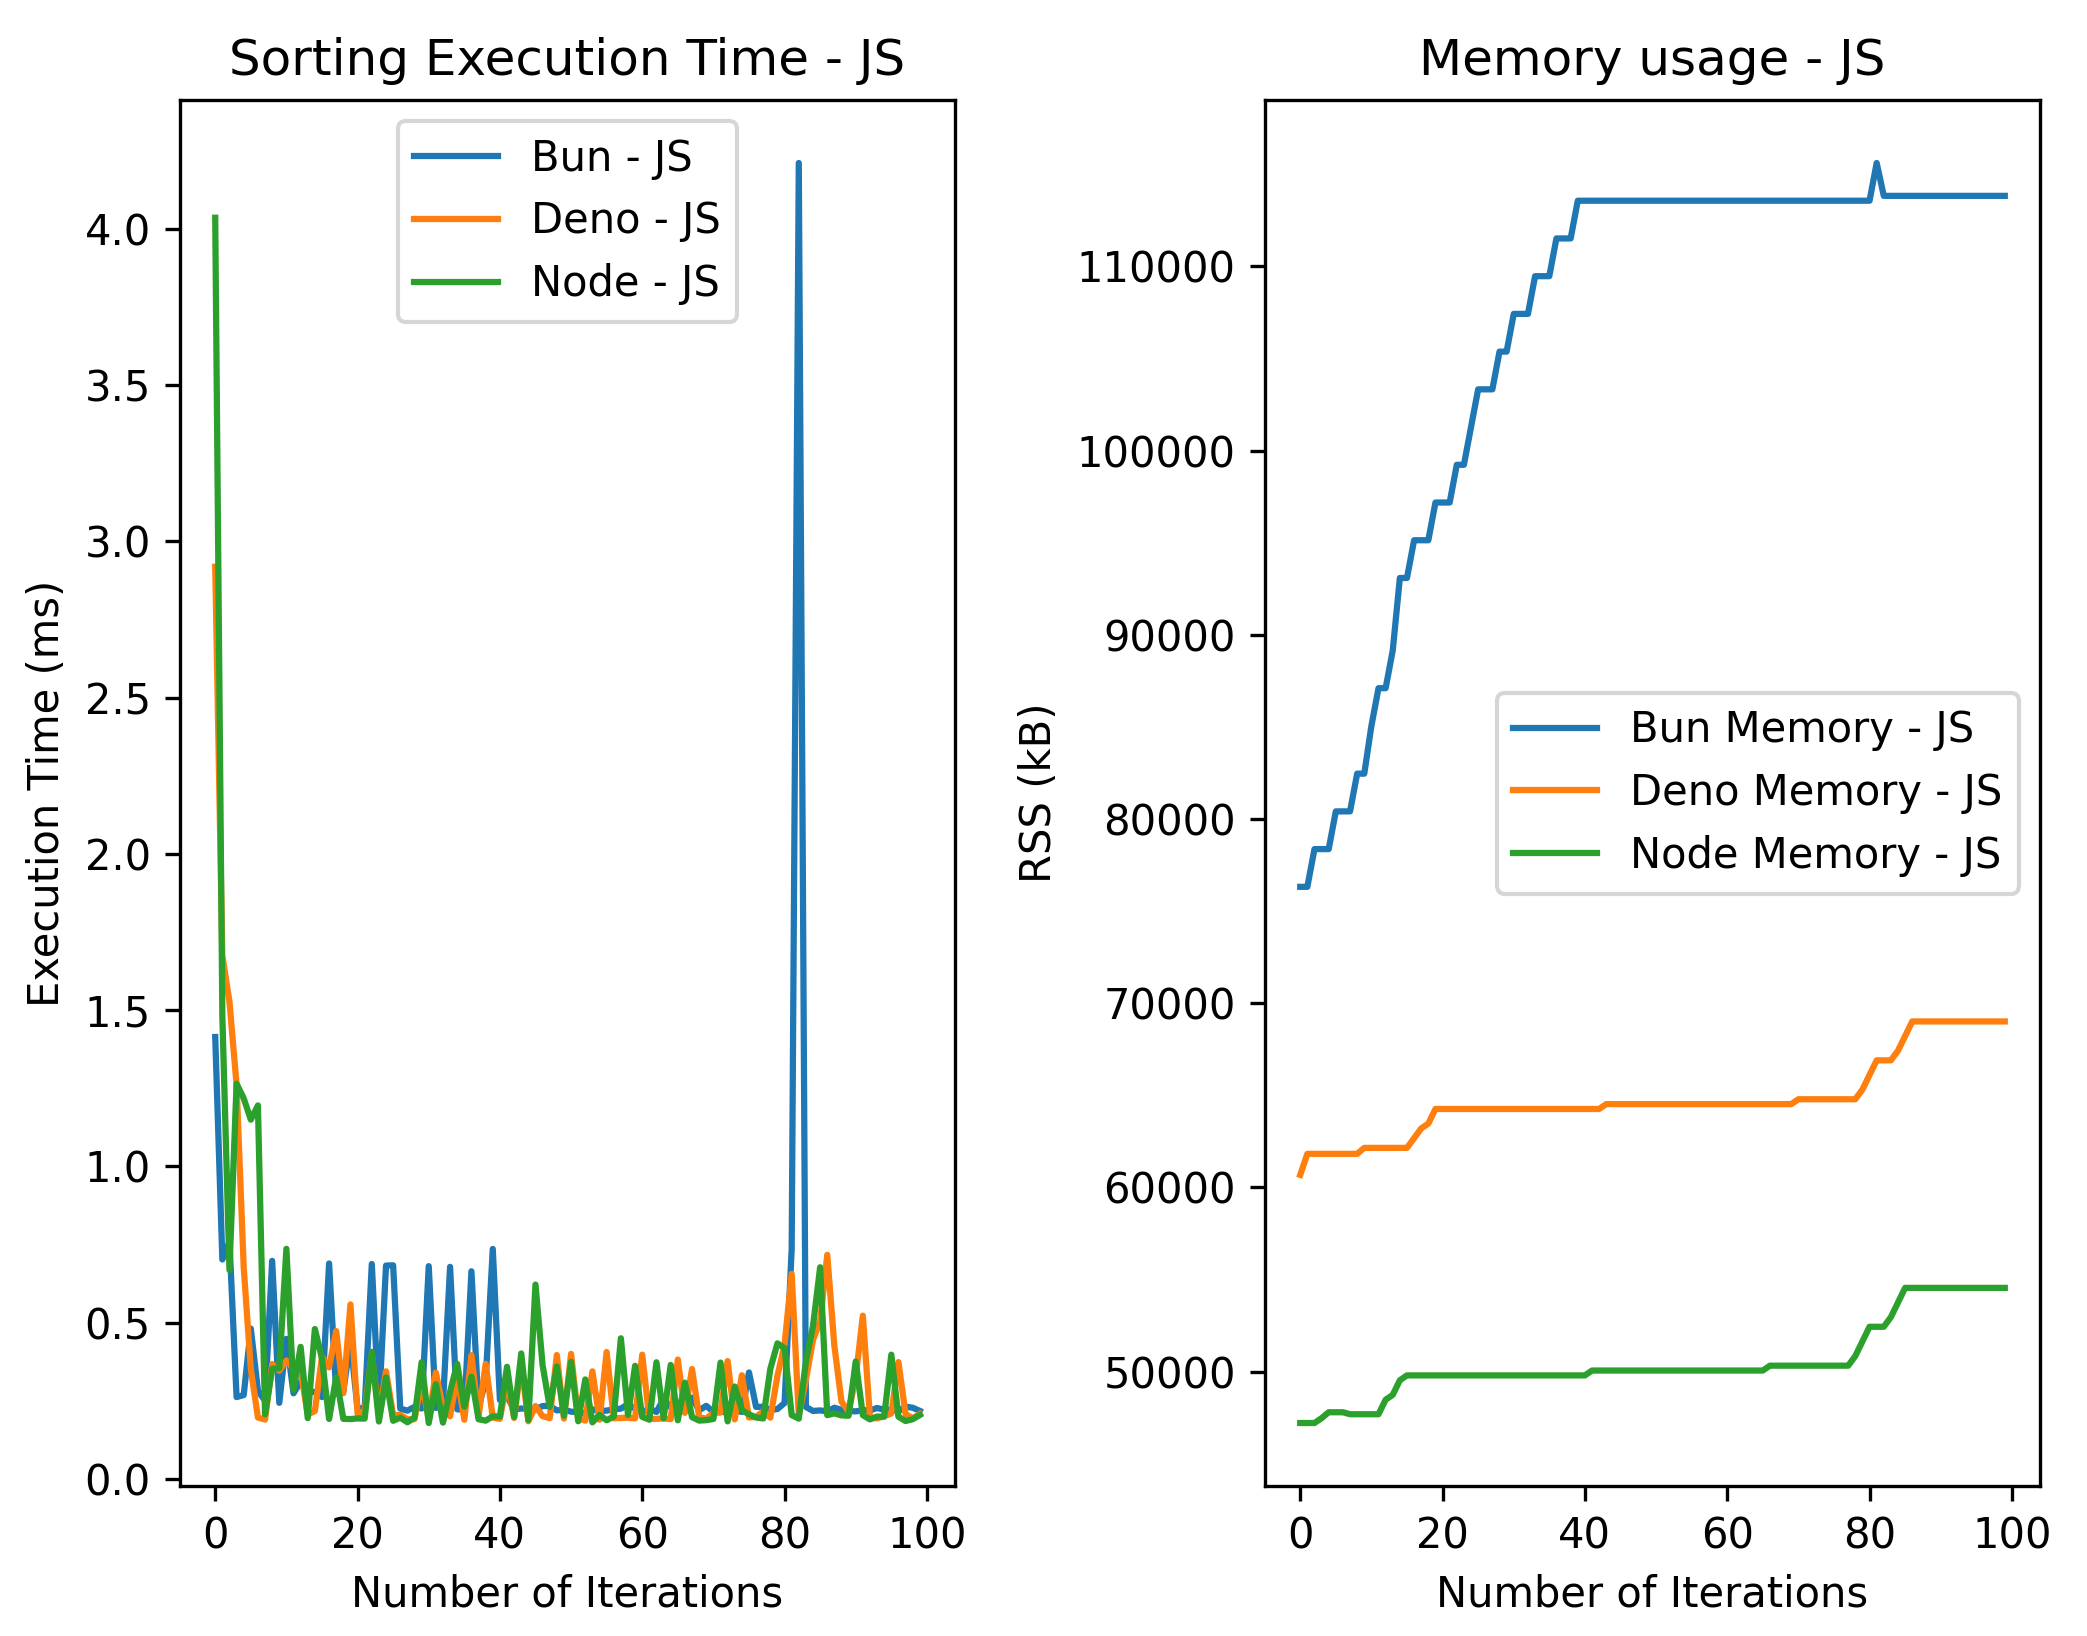
\includegraphics[width=0.68\textwidth]{Figures/sorting/sorting_quick_100_1000_js.png}
  \caption{Wyniki eksperymentów dla algorytmu sortowania szybkiego dla 100 iteracji i 1000 elementów - po lewej czas wykonania jednorazowego testu w milisekundach, po prawej ilość zajmowanej pamięci w kilobajtach (kB)}
  \label{fig:quick_sorting_e1}
\end{figure}

Na rysunku \ref{fig:quick_sorting_e1_ts} przedstawiono wyniki eksperymentów dla algorytmu sortowania szybkiego dla 100 iteracji i 1000 elementów napisanego w języku TypeScript. Na wykresie przedstawiono czas wykonania jednorazowego testu w milisekundach oraz ilość zajmowanej pamięci w kilobajtach (kB).

\begin{figure}[H]
  \centering
  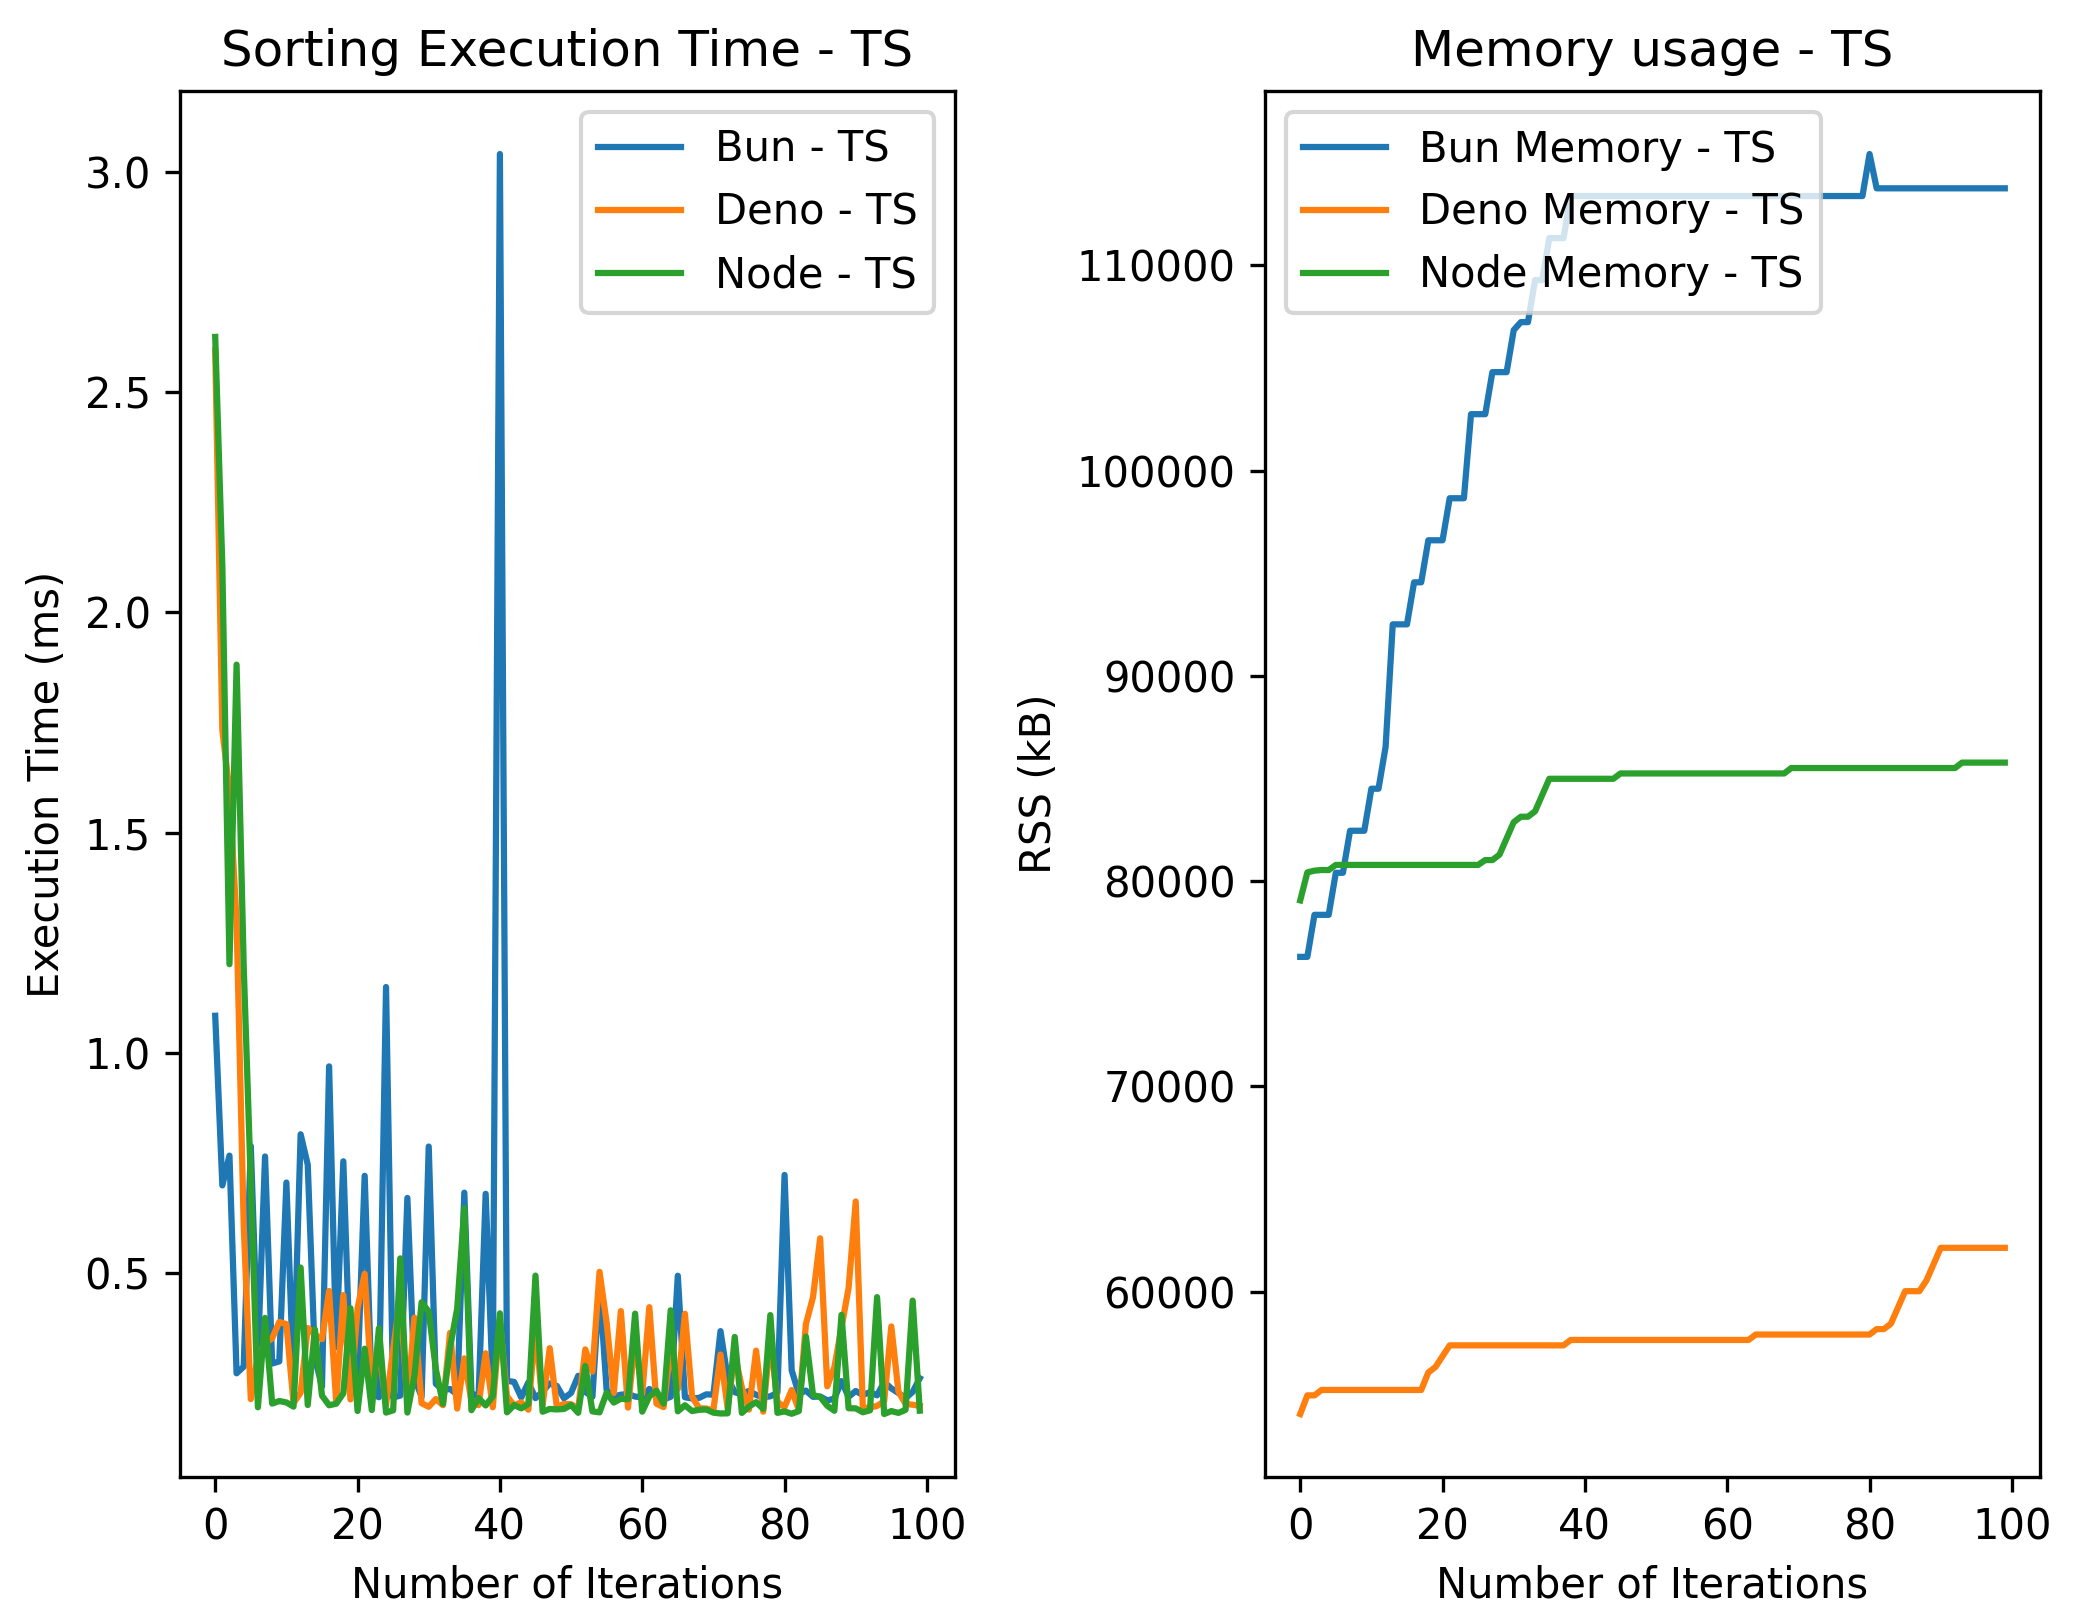
\includegraphics[width=0.68\textwidth]{Figures/sorting/sorting_quick_100_1000_ts.png}
  \caption{Wyniki eksperymentów dla algorytmu sortowania szybkiego dla 100 iteracji i 1000 elementów - po lewej czas wykonania jednorazowego testu w milisekundach, po prawej ilość zajmowanej pamięci w kilobajtach (kB)}
  \label{fig:quick_sorting_e1_ts}
\end{figure}

Na rysunku \ref{fig:quick_sorting_e2} przedstawiono wyniki eksperymentów dla algorytmu sortowania szybkiego dla 100 iteracji i 1000 elementów napisanego w języku JavaScript. Na wykresie przedstawiono czas wykonania jednorazowego testu w milisekundach oraz ilość zajmowanej pamięci w kilobajtach (kB).

\begin{figure}[H]
  \centering
  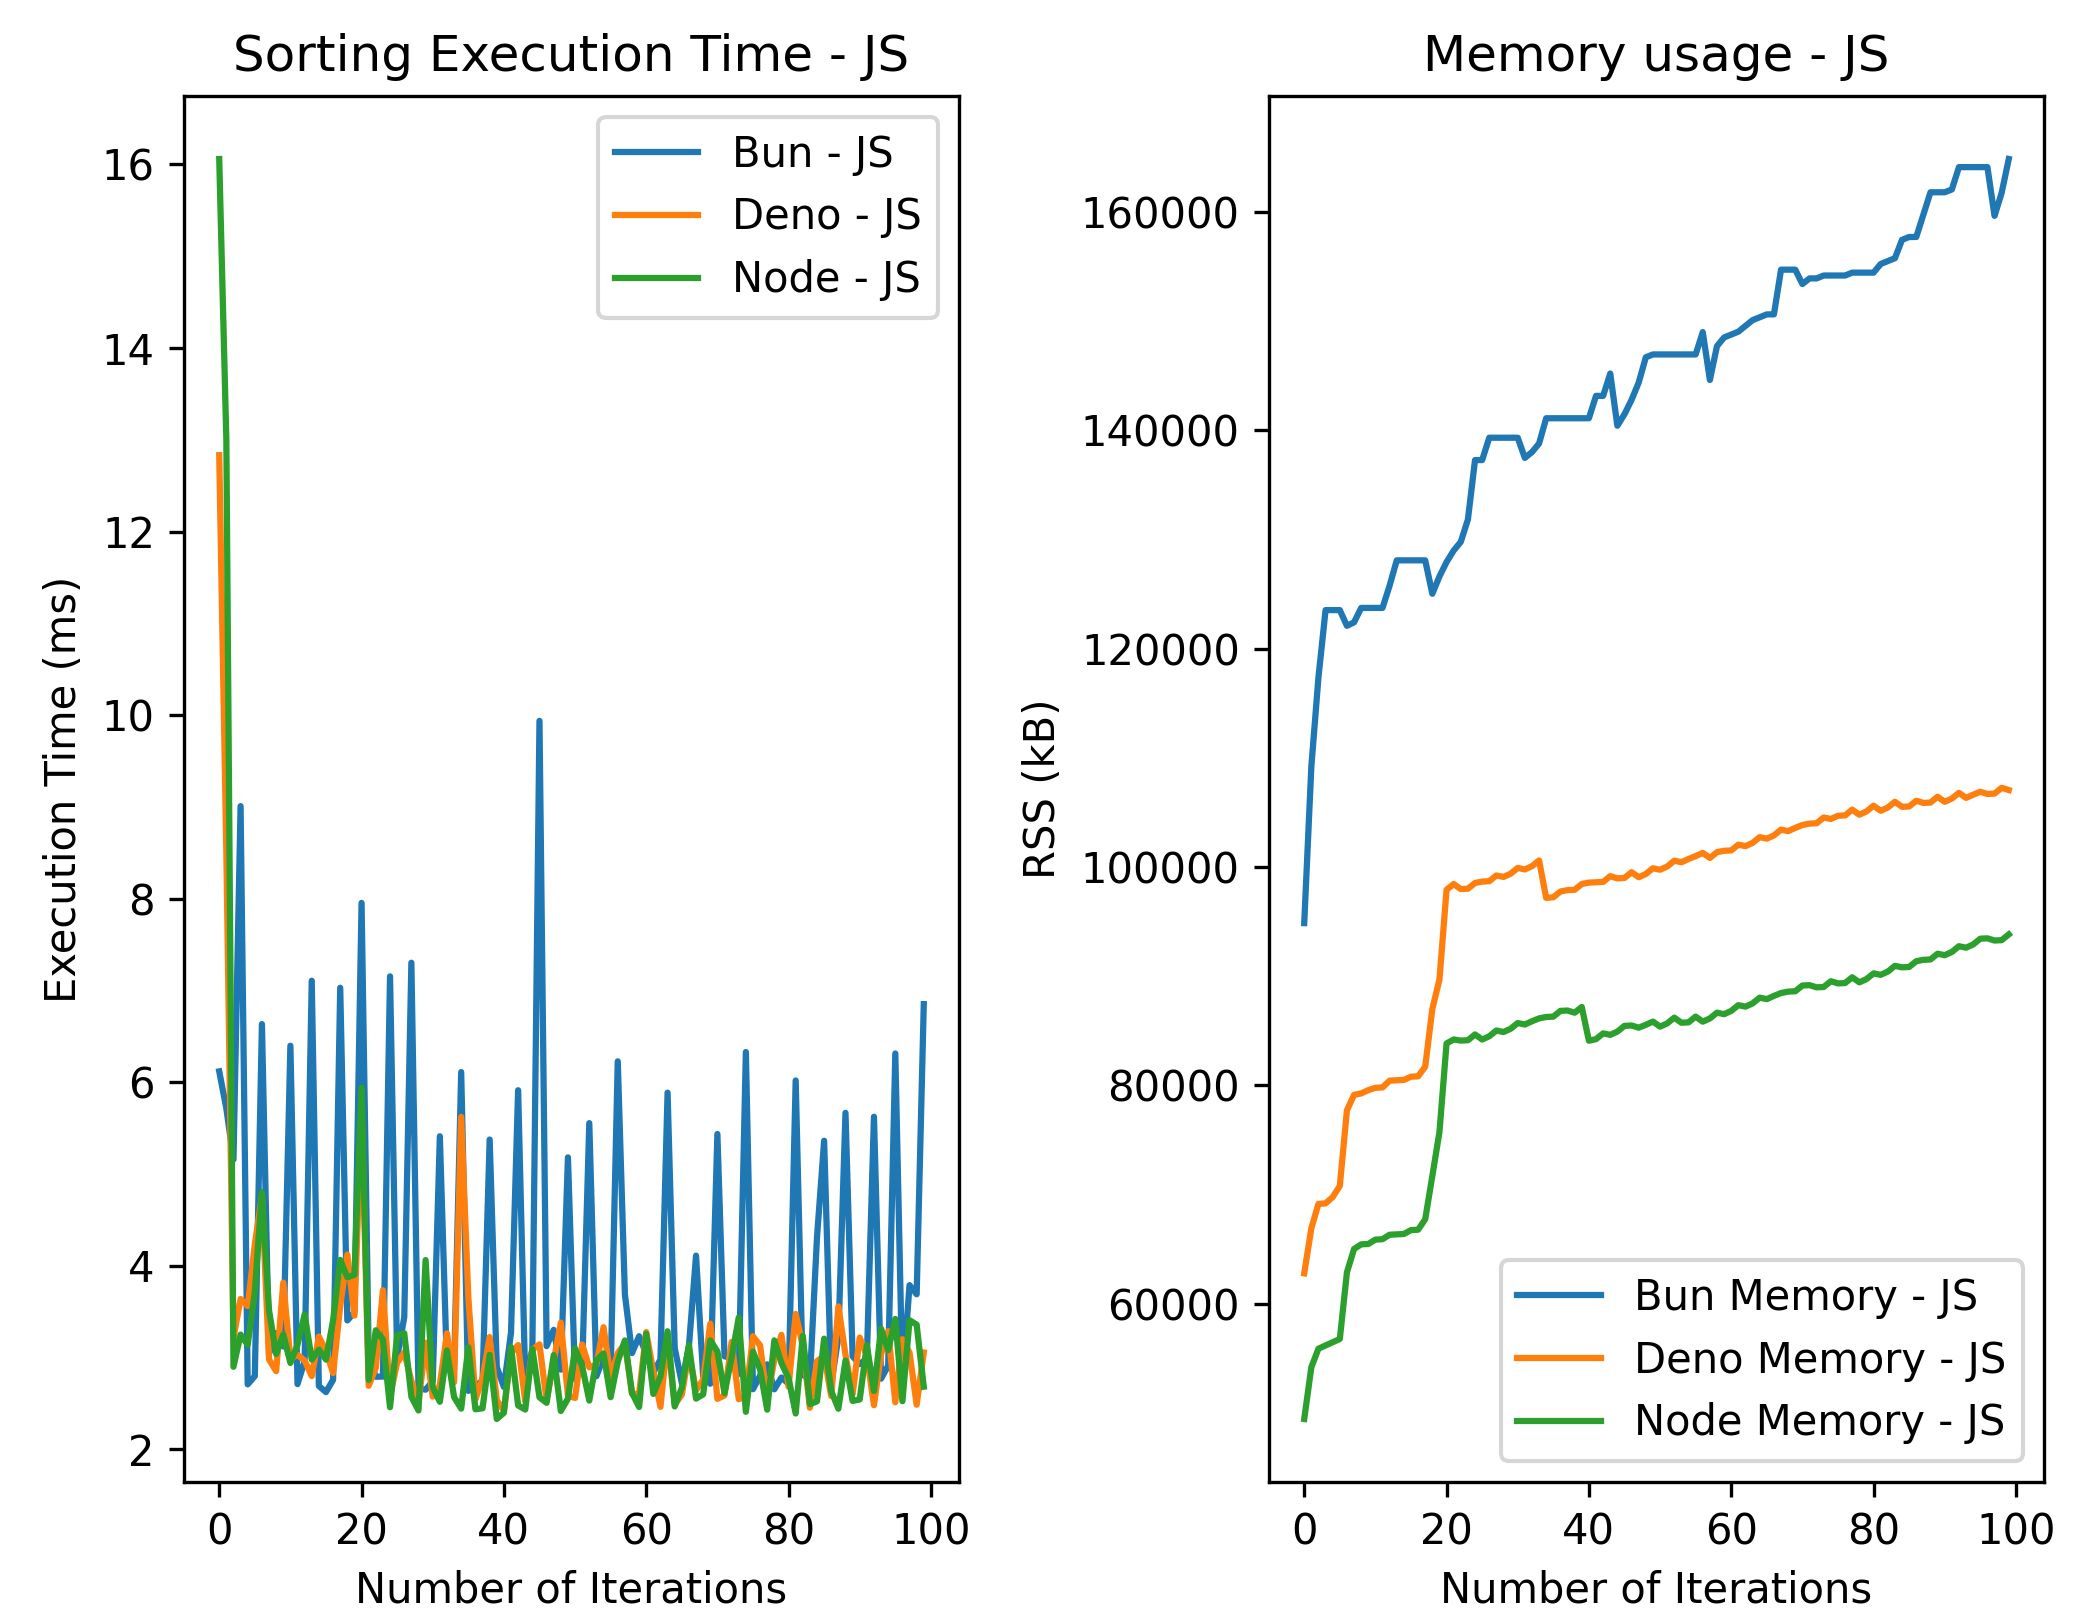
\includegraphics[width=0.68\textwidth]{Figures/sorting/sorting_quick_100_10000_js.png}
  \caption{Wyniki eksperymentów dla algorytmu sortowania szybkiego dla 100 iteracji i 10000 elementów - po lewej czas wykonania jednorazowego testu w milisekundach, po prawej ilość zajmowanej pamięci w kilobajtach (kB)}
  \label{fig:quick_sorting_e2}
\end{figure}

Na rysunku \ref{fig:quick_sorting_e2_ts} przedstawiono wyniki eksperymentów dla algorytmu sortowania szybkiego dla 100 iteracji i 10000 elementów napisanego w języku TypeScript. Na wykresie przedstawiono czas wykonania jednorazowego testu w milisekundach oraz ilość zajmowanej pamięci w kilobajtach (kB).

\begin{figure}[H]
  \centering
  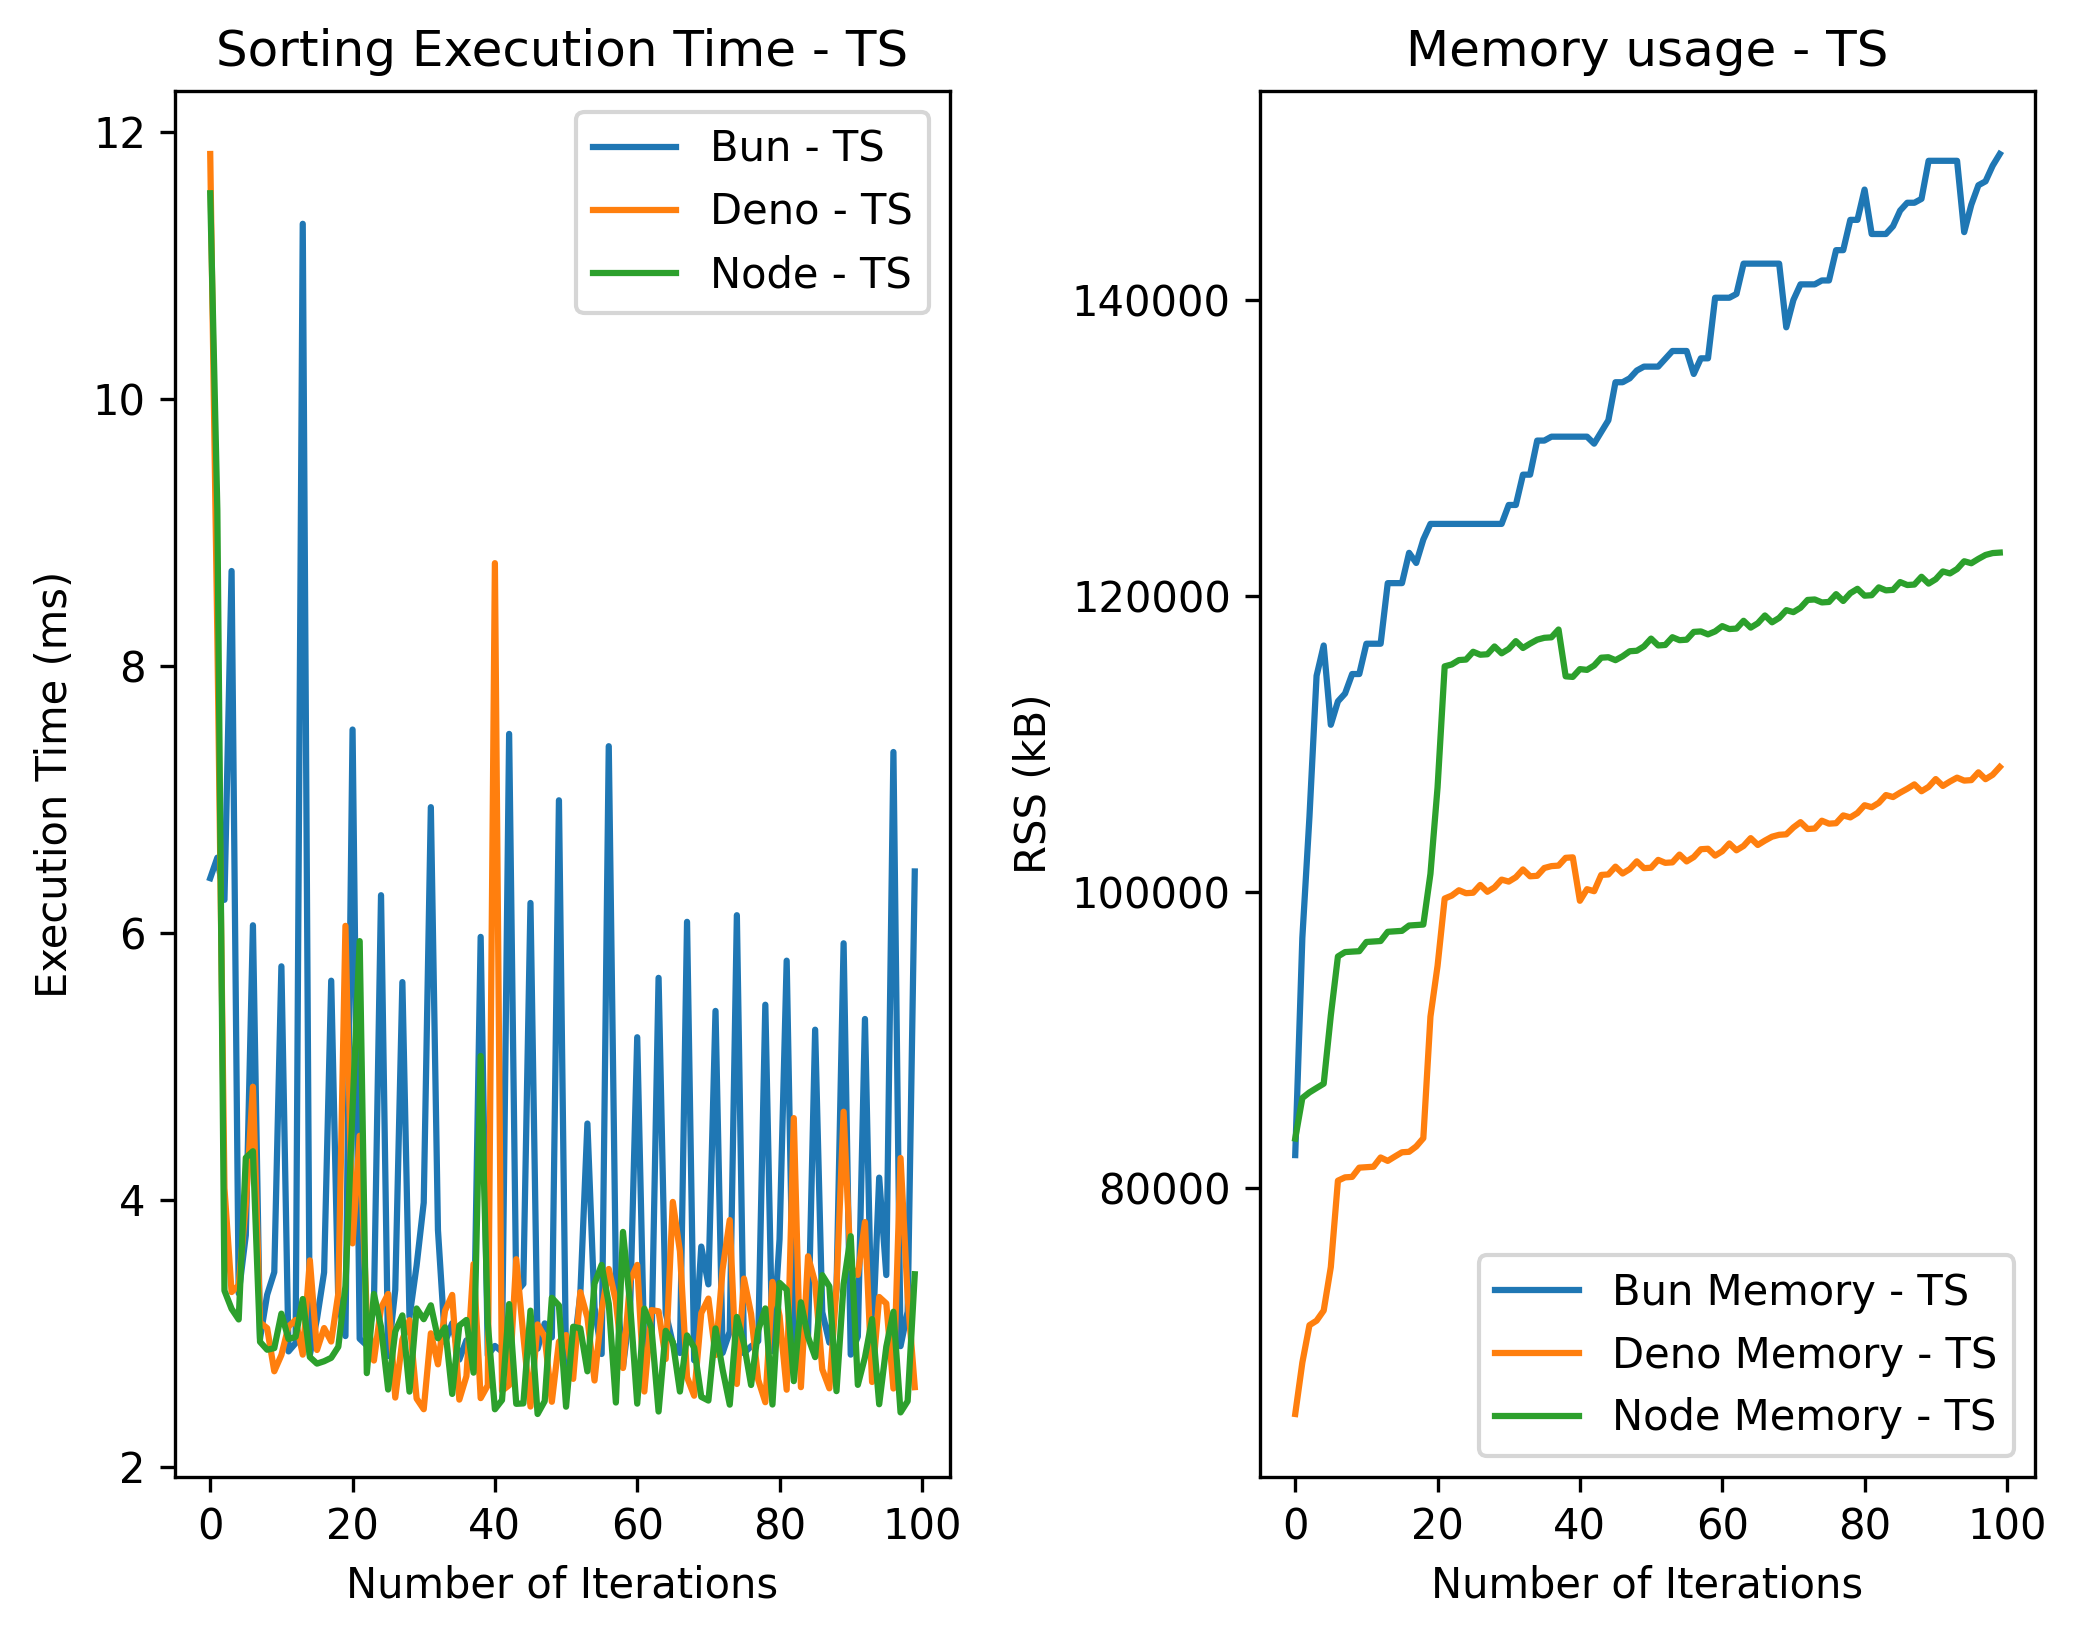
\includegraphics[width=0.68\textwidth]{Figures/sorting/sorting_quick_100_10000_ts.png}
  \caption{Wyniki eksperymentów dla algorytmu sortowania szybkiego dla 100 iteracji i 10000 elementów - po lewej czas wykonania jednorazowego testu w milisekundach, po prawej ilość zajmowanej pamięci w kilobajtach (kB)}
  \label{fig:quick_sorting_e2_ts}
\end{figure}

Na rysunku \ref{fig:quick_sorting_e3} przedstawiono wyniki eksperymentów dla algorytmu sortowania szybkiego dla 1000 iteracji i 1000 elementów napisanego w języku JavaScript. Na wykresie przedstawiono czas wykonania jednorazowego testu w milisekundach oraz ilość zajmowanej pamięci w kilobajtach (kB).

\begin{figure}[H]
  \centering
  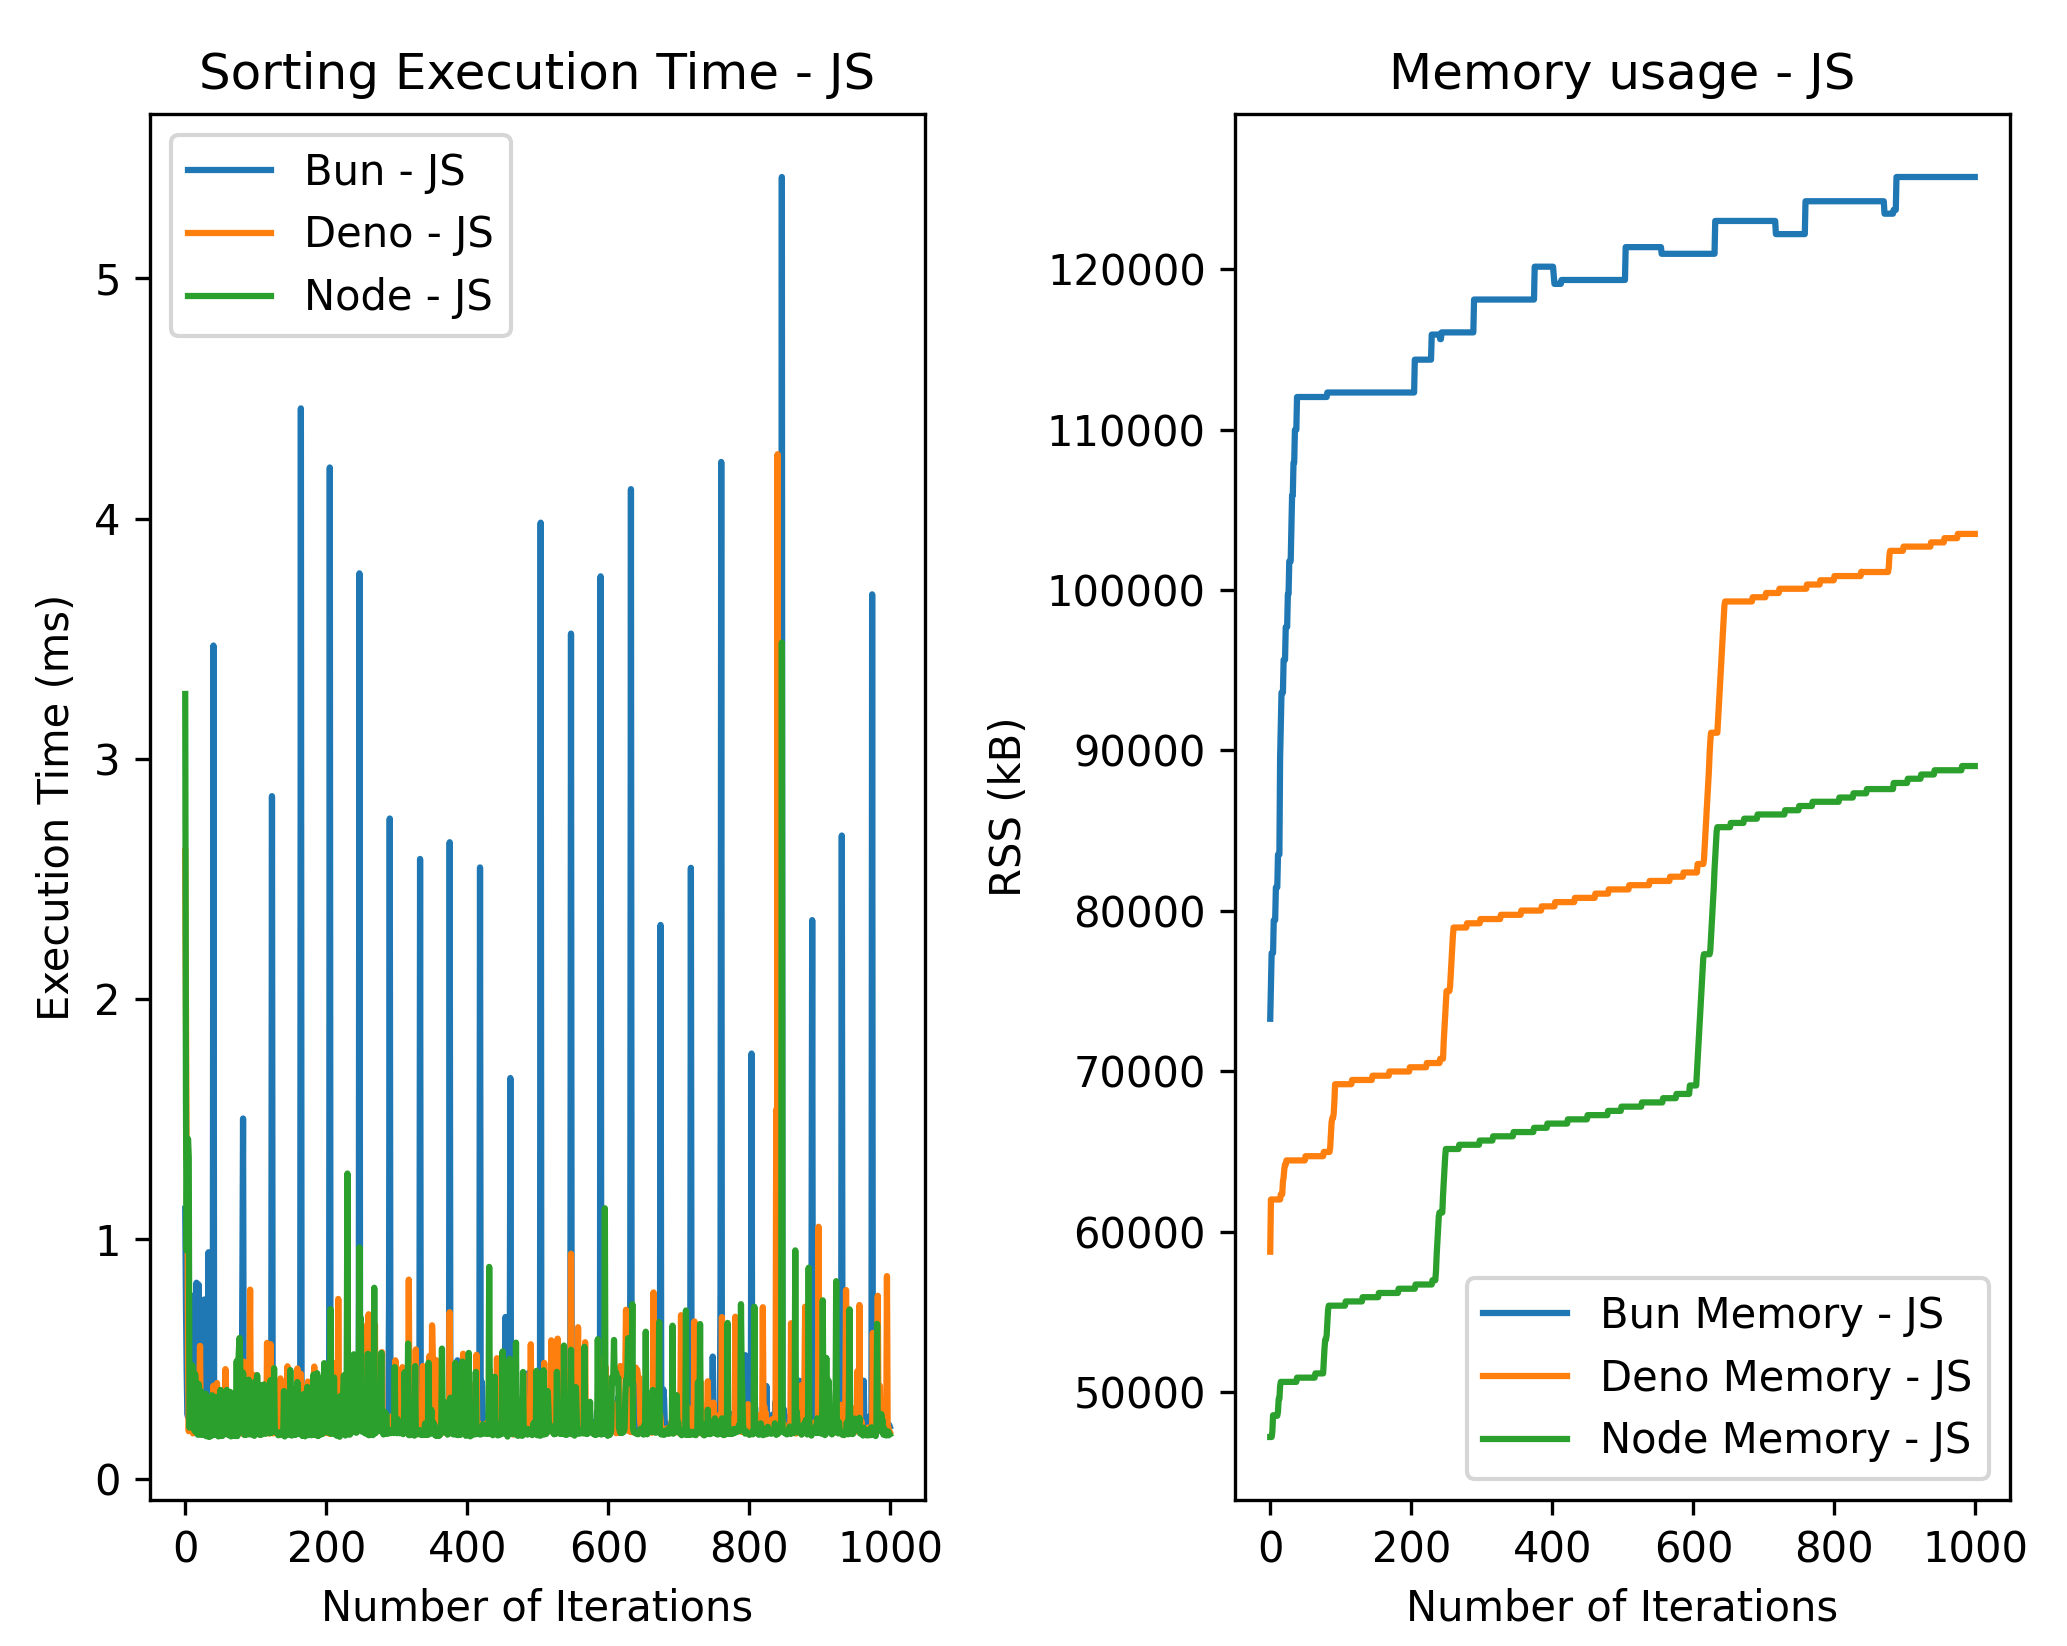
\includegraphics[width=0.68\textwidth]{Figures/sorting/sorting_quick_1000_1000_js.png}
  \caption{Wyniki eksperymentów dla algorytmu sortowania szybkiego dla 1000 iteracji i 1000 elementów - po lewej czas wykonania jednorazowego testu w milisekundach, po prawej ilość zajmowanej pamięci w kilobajtach (kB)}
  \label{fig:quick_sorting_e3}
\end{figure}

Na rysunku \ref{fig:quick_sorting_e3_ts} przedstawiono wyniki eksperymentów dla algorytmu sortowania szybkiego dla 1000 iteracji i 1000 elementów napisanego w języku TypeScript. Na wykresie przedstawiono czas wykonania jednorazowego testu w milisekundach oraz ilość zajmowanej pamięci w kilobajtach (kB).

\begin{figure}[H]
  \centering
  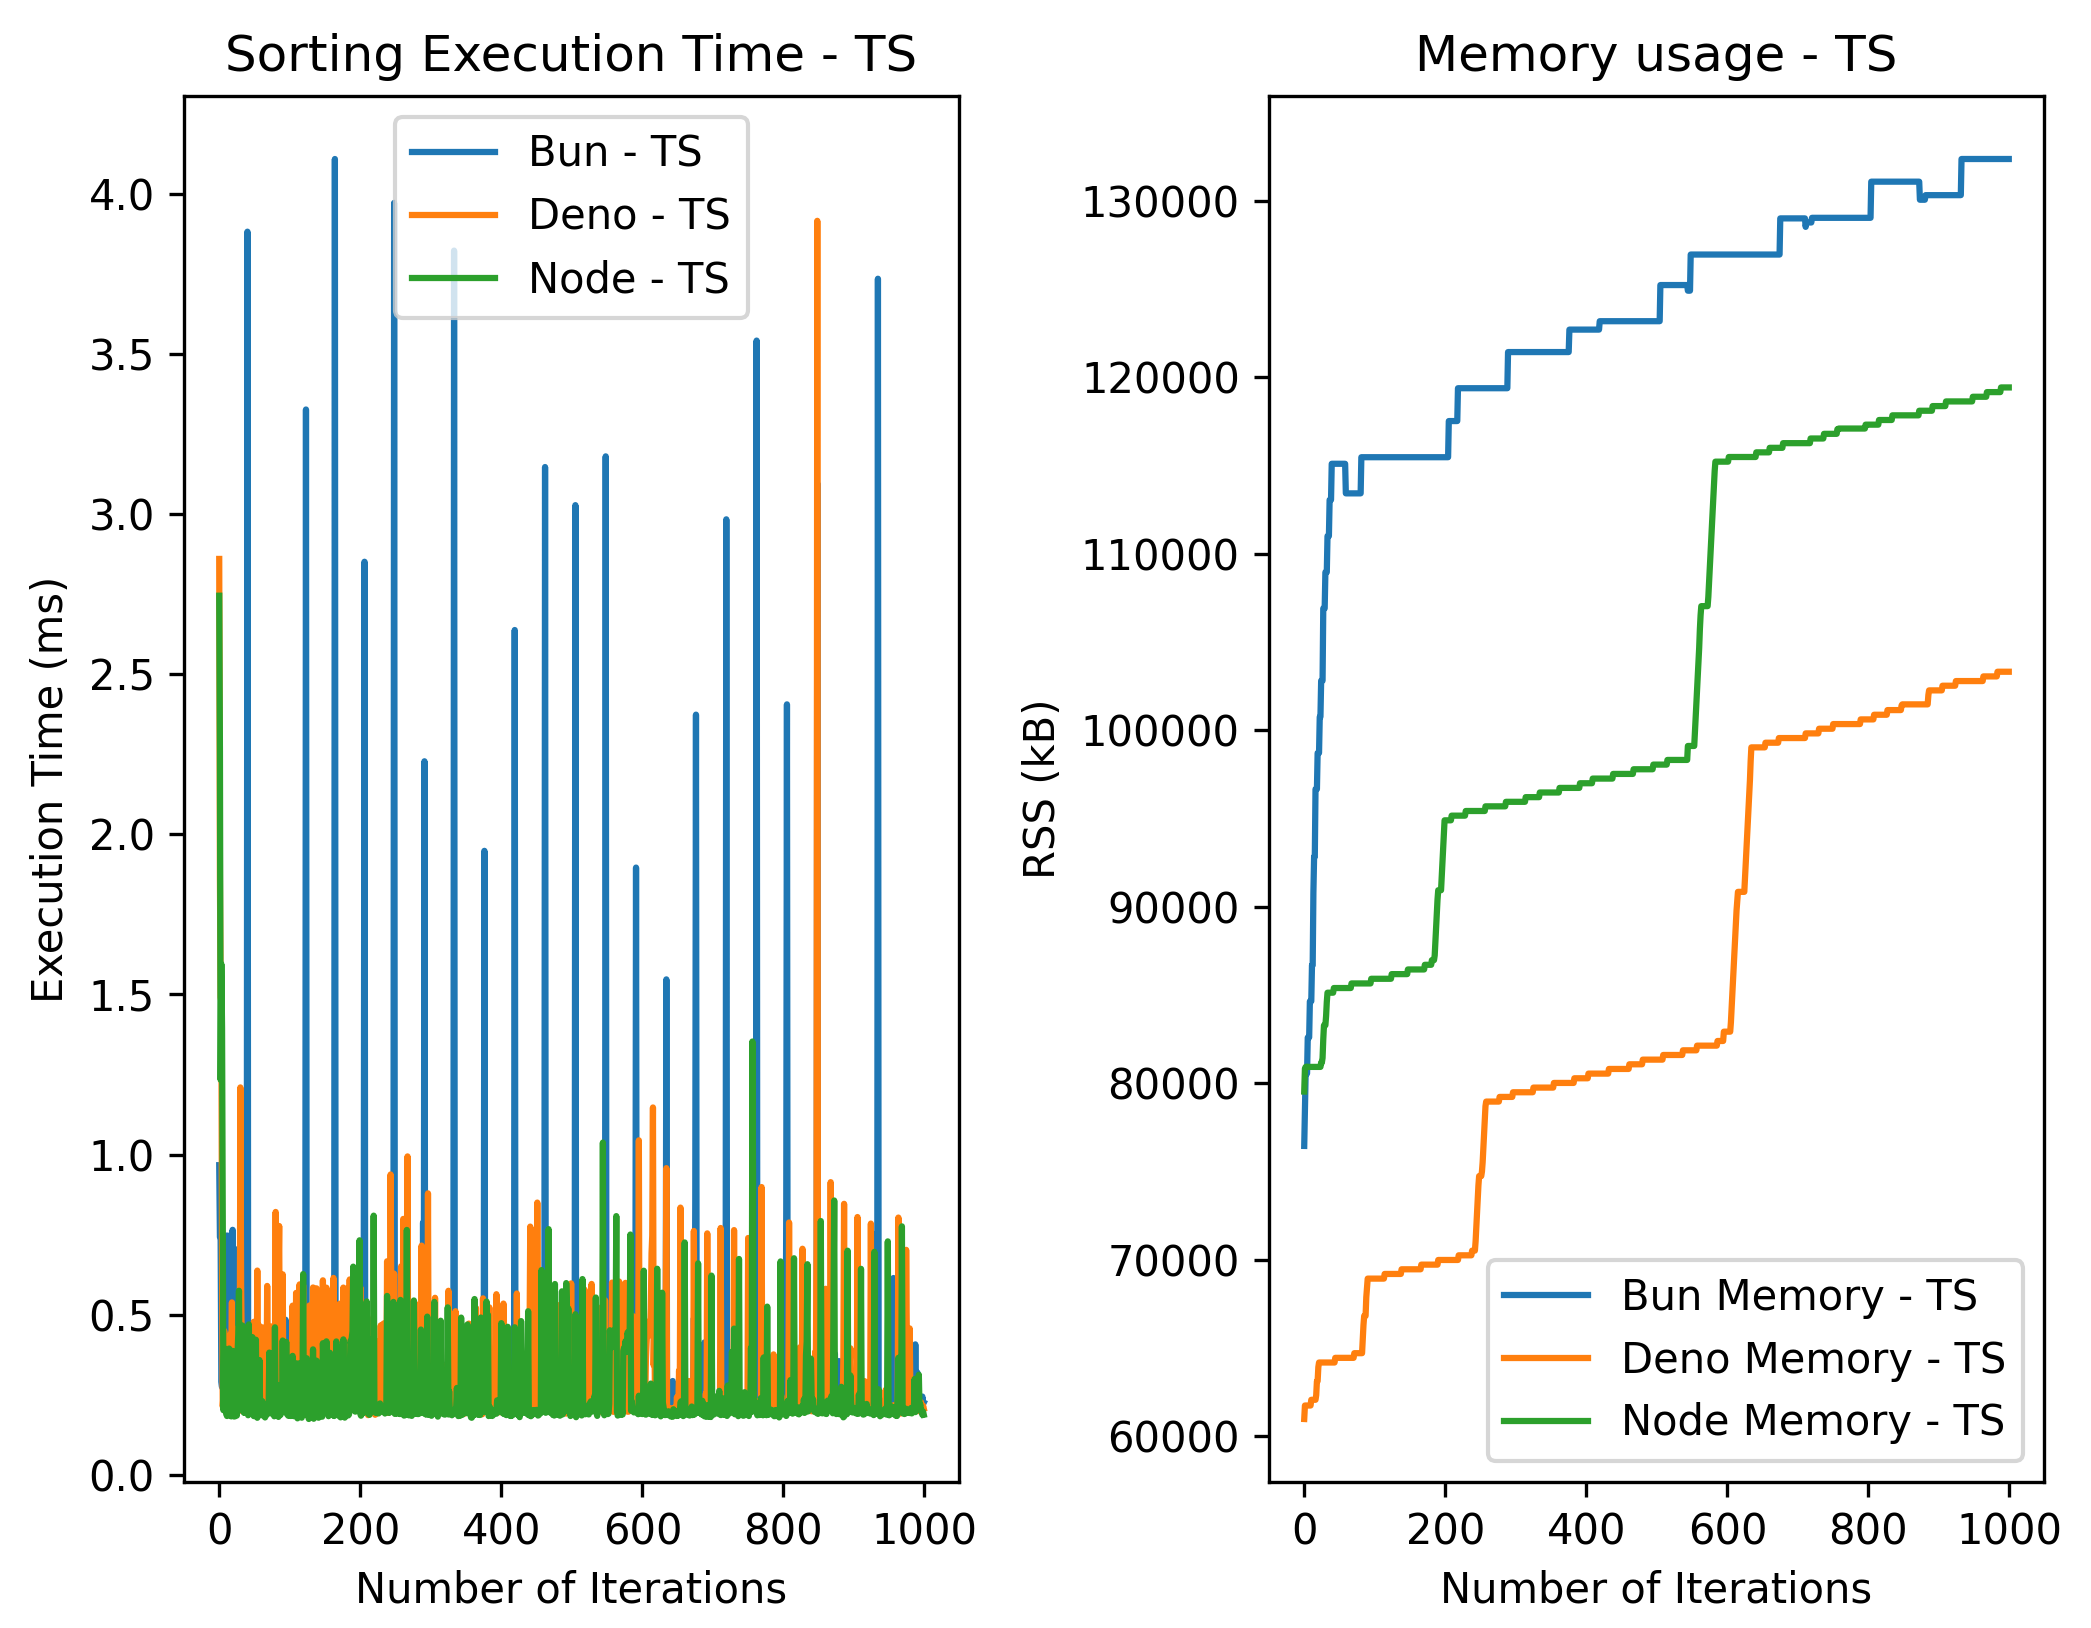
\includegraphics[width=0.68\textwidth]{Figures/sorting/sorting_quick_1000_1000_ts.png}
  \caption{Wyniki eksperymentów dla algorytmu sortowania szybkiego dla 100 iteracji i 1000 elementów - po lewej czas wykonania jednorazowego testu w milisekundach, po prawej ilość zajmowanej pamięci w kilobajtach (kB)}
  \label{fig:quick_sorting_e3_ts}
\end{figure}

Na rysunku \ref{fig:quick_sorting_e4} przedstawiono wyniki eksperymentów dla algorytmu sortowania szybkiego dla 100 iteracji i 1000 elementów napisanego w języku JavaScript. Na wykresie przedstawiono czas wykonania jednorazowego testu w milisekundach oraz ilość zajmowanej pamięci w kilobajtach (kB).

\begin{figure}[H]
  \centering
  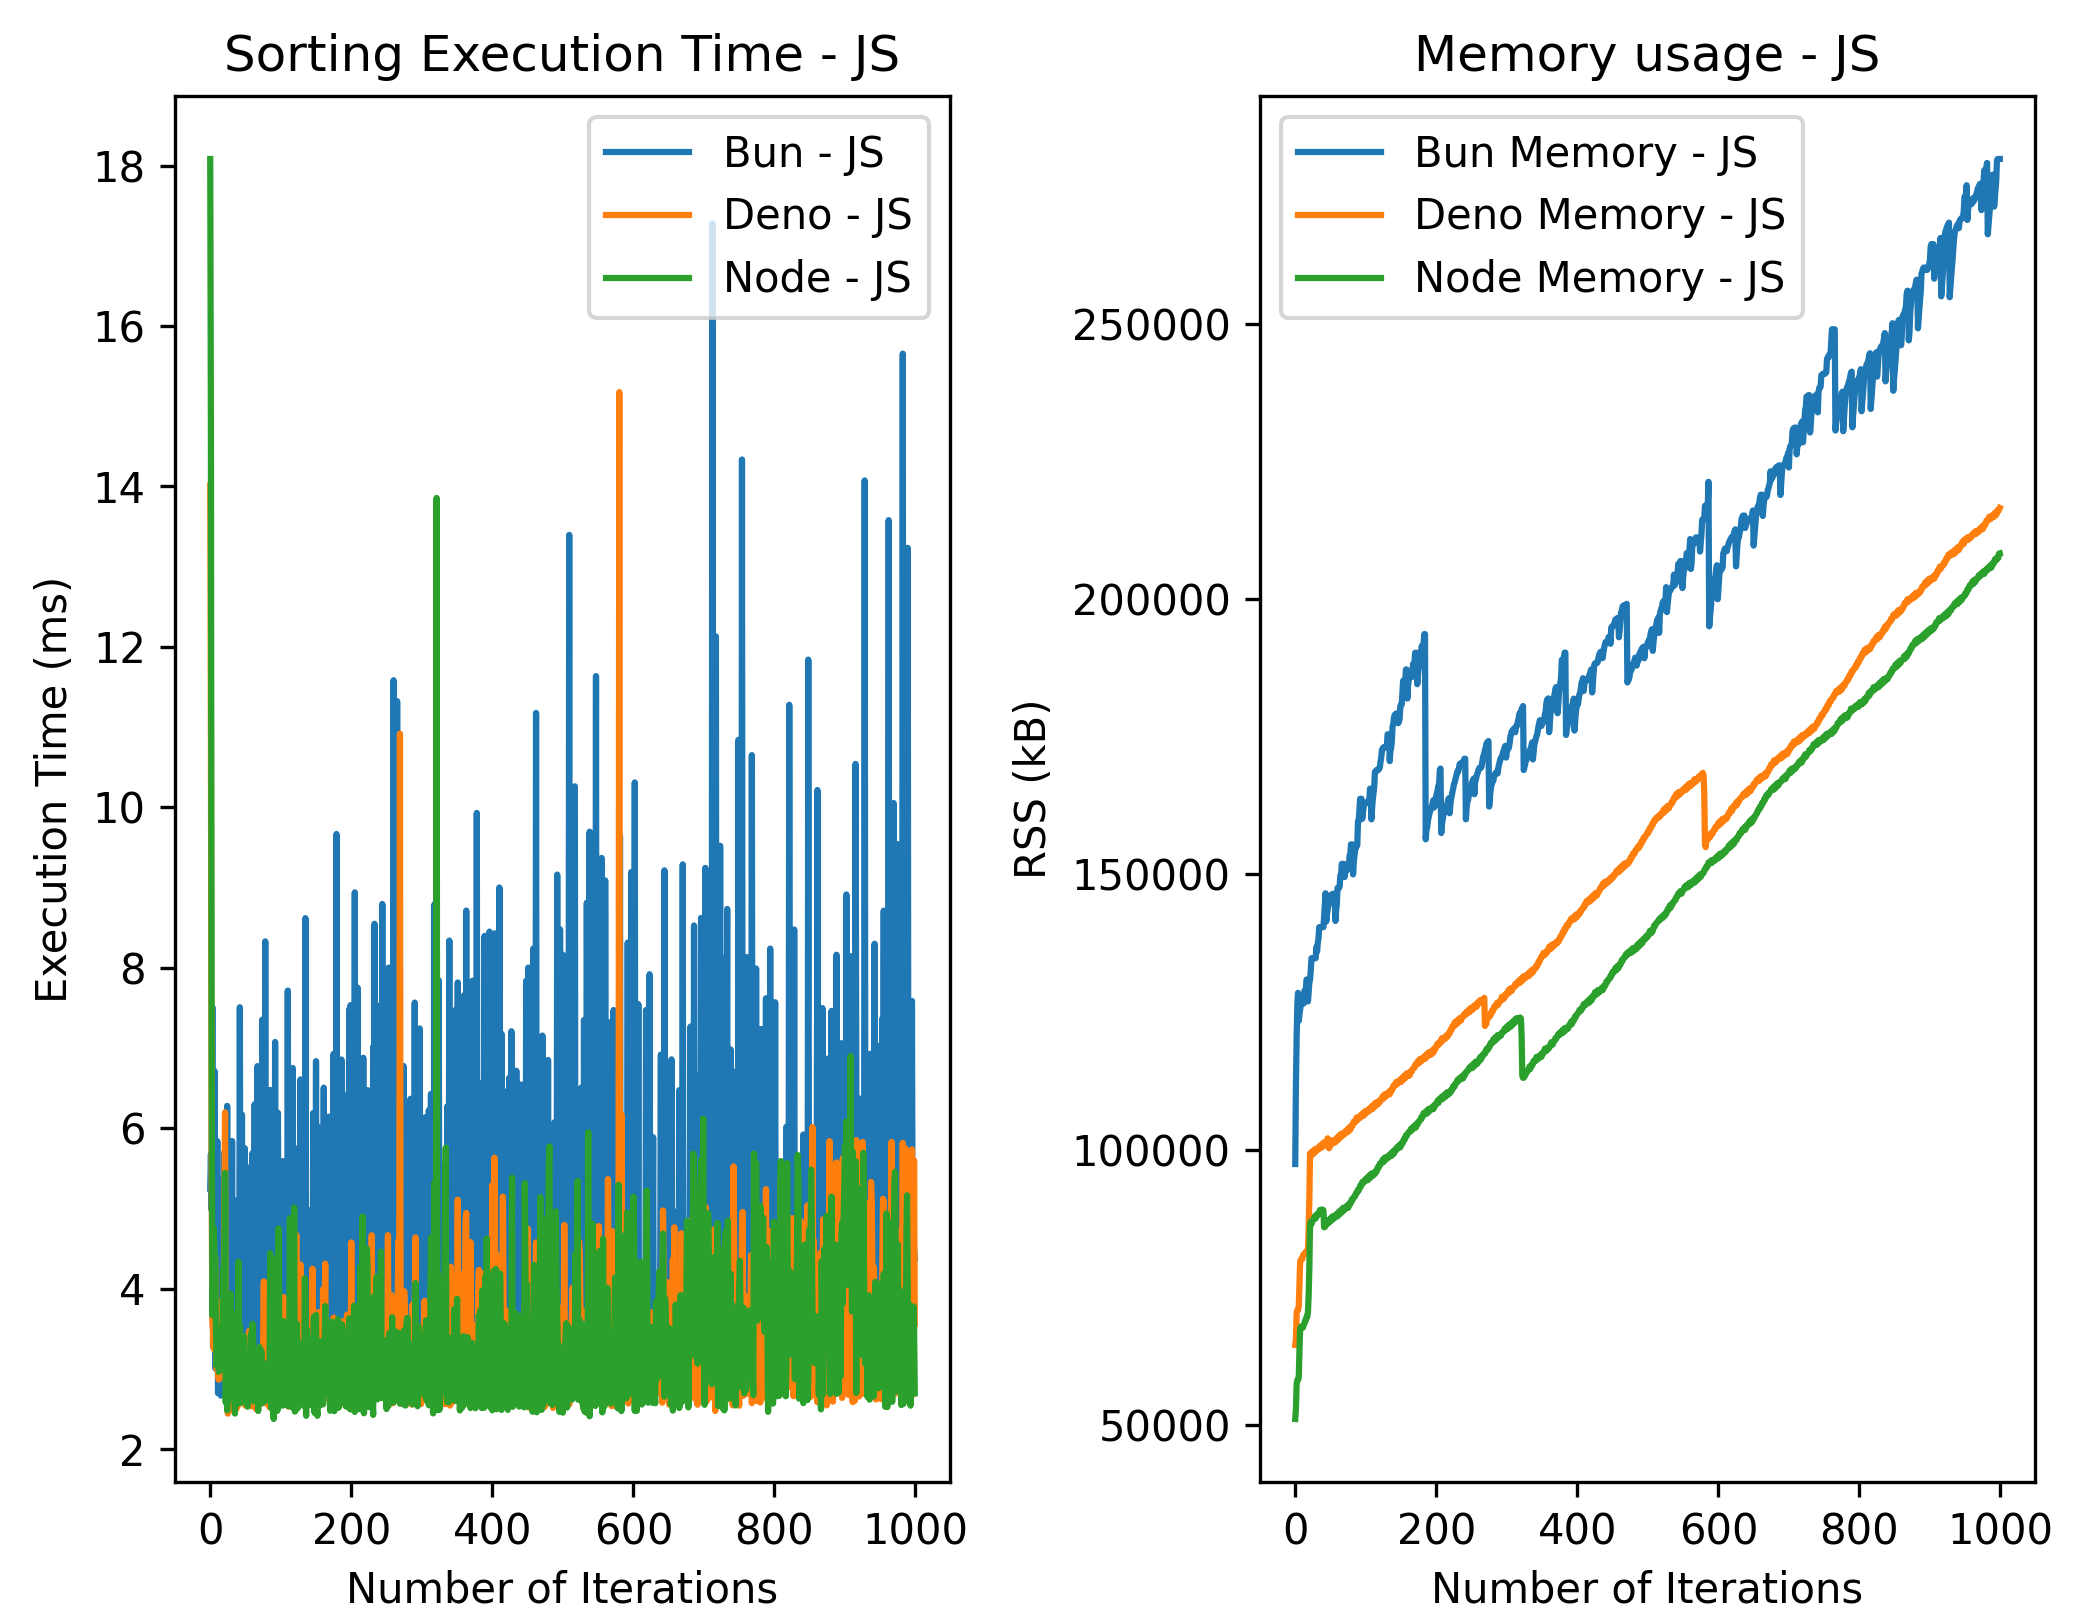
\includegraphics[width=0.68\textwidth]{Figures/sorting/sorting_quick_1000_10000_js.png}
  \caption{Wyniki eksperymentów dla algorytmu sortowania szybkiego dla 100 iteracji i 10000 elementów - po lewej czas wykonania jednorazowego testu w milisekundach, po prawej ilość zajmowanej pamięci w kilobajtach (kB)}
  \label{fig:quick_sorting_e4}
\end{figure}

Na rysunku \ref{fig:quick_sorting_e4_ts} przedstawiono wyniki eksperymentów dla algorytmu sortowania szybkiego dla 100 iteracji i 10000 elementów napisanego w języku TypeScript. Na wykresie przedstawiono czas wykonania jednorazowego testu w milisekundach oraz ilość zajmowanej pamięci w kilobajtach (kB).

\begin{figure}[H]
  \centering
  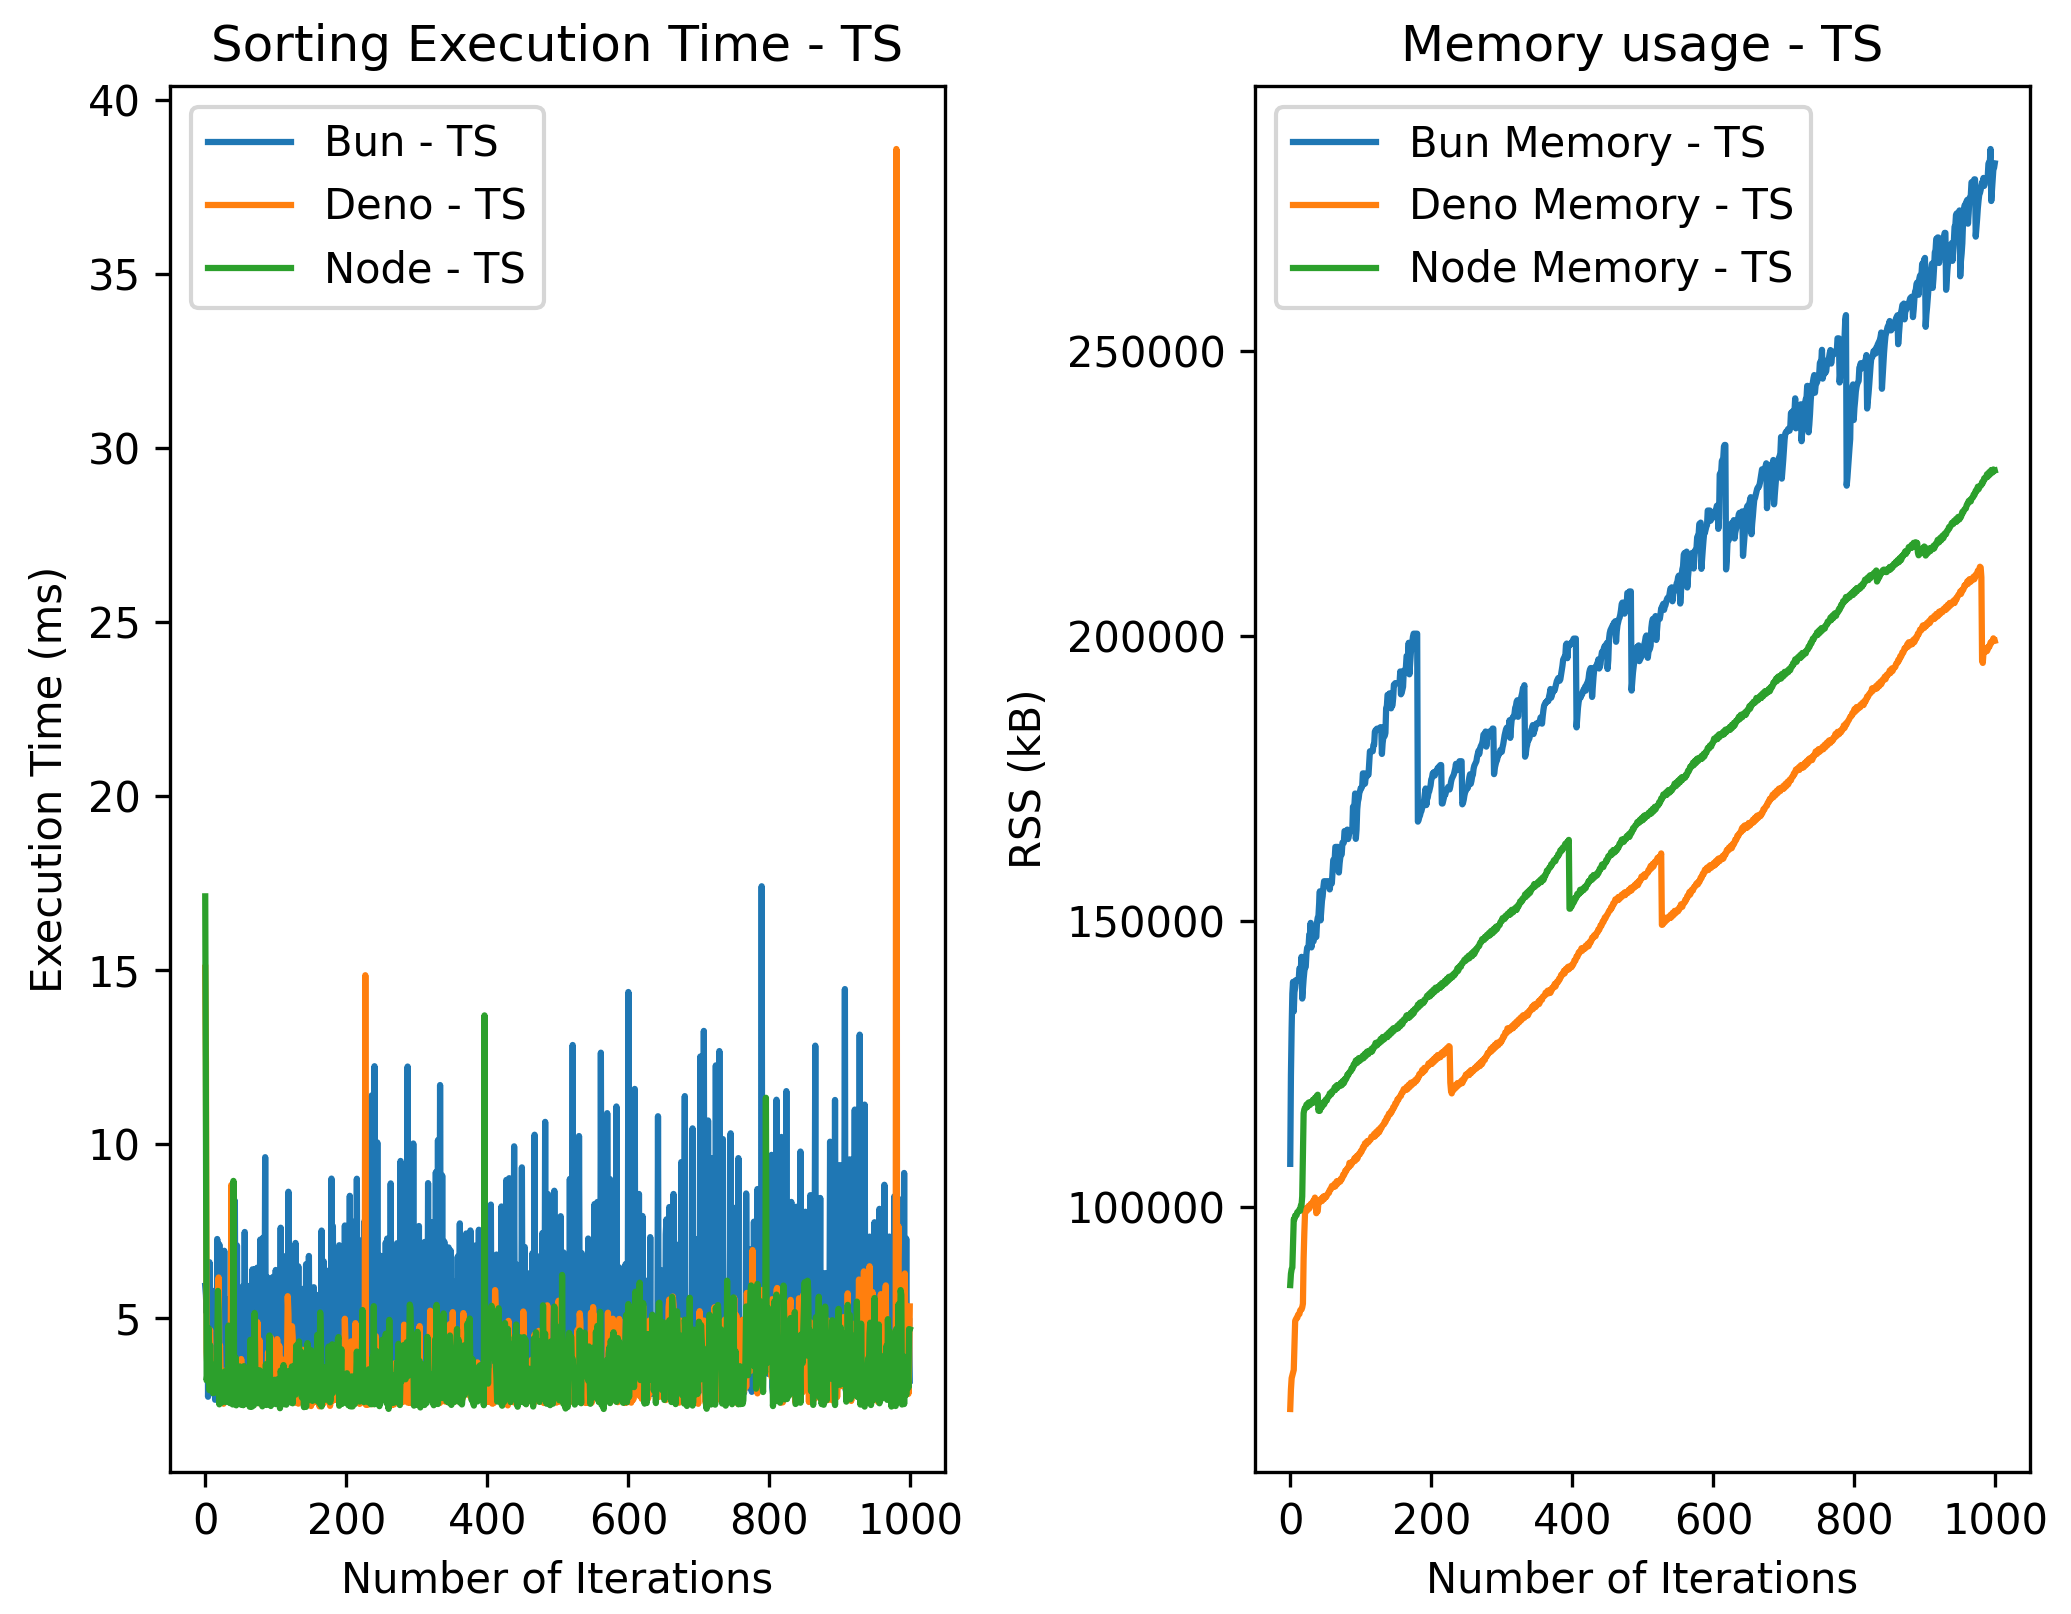
\includegraphics[width=0.68\textwidth]{Figures/sorting/sorting_quick_1000_10000_ts.png}
  \caption{Wyniki eksperymentów dla algorytmu sortowania szybkiego dla 100 iteracji i 10000 elementów - po lewej czas wykonania jednorazowego testu w milisekundach, po prawej ilość zajmowanej pamięci w kilobajtach (kB)}
  \label{fig:quick_sorting_e4_ts}
\end{figure}

\subsubsection{Wyniki - sortowanie pozycyjne}
Na rysunku \ref{fig:radix_sorting_e1} przedstawiono wyniki eksperymentów dla algorytmu sortowania pozycyjnego dla 100 iteracji i 1000 elementów napisanego w języku JavaScript. Na wykresie przedstawiono czas wykonania jednorazowego testu w milisekundach oraz ilość zajmowanej pamięci w kilobajtach (kB).

\begin{figure}[H]
  \centering
  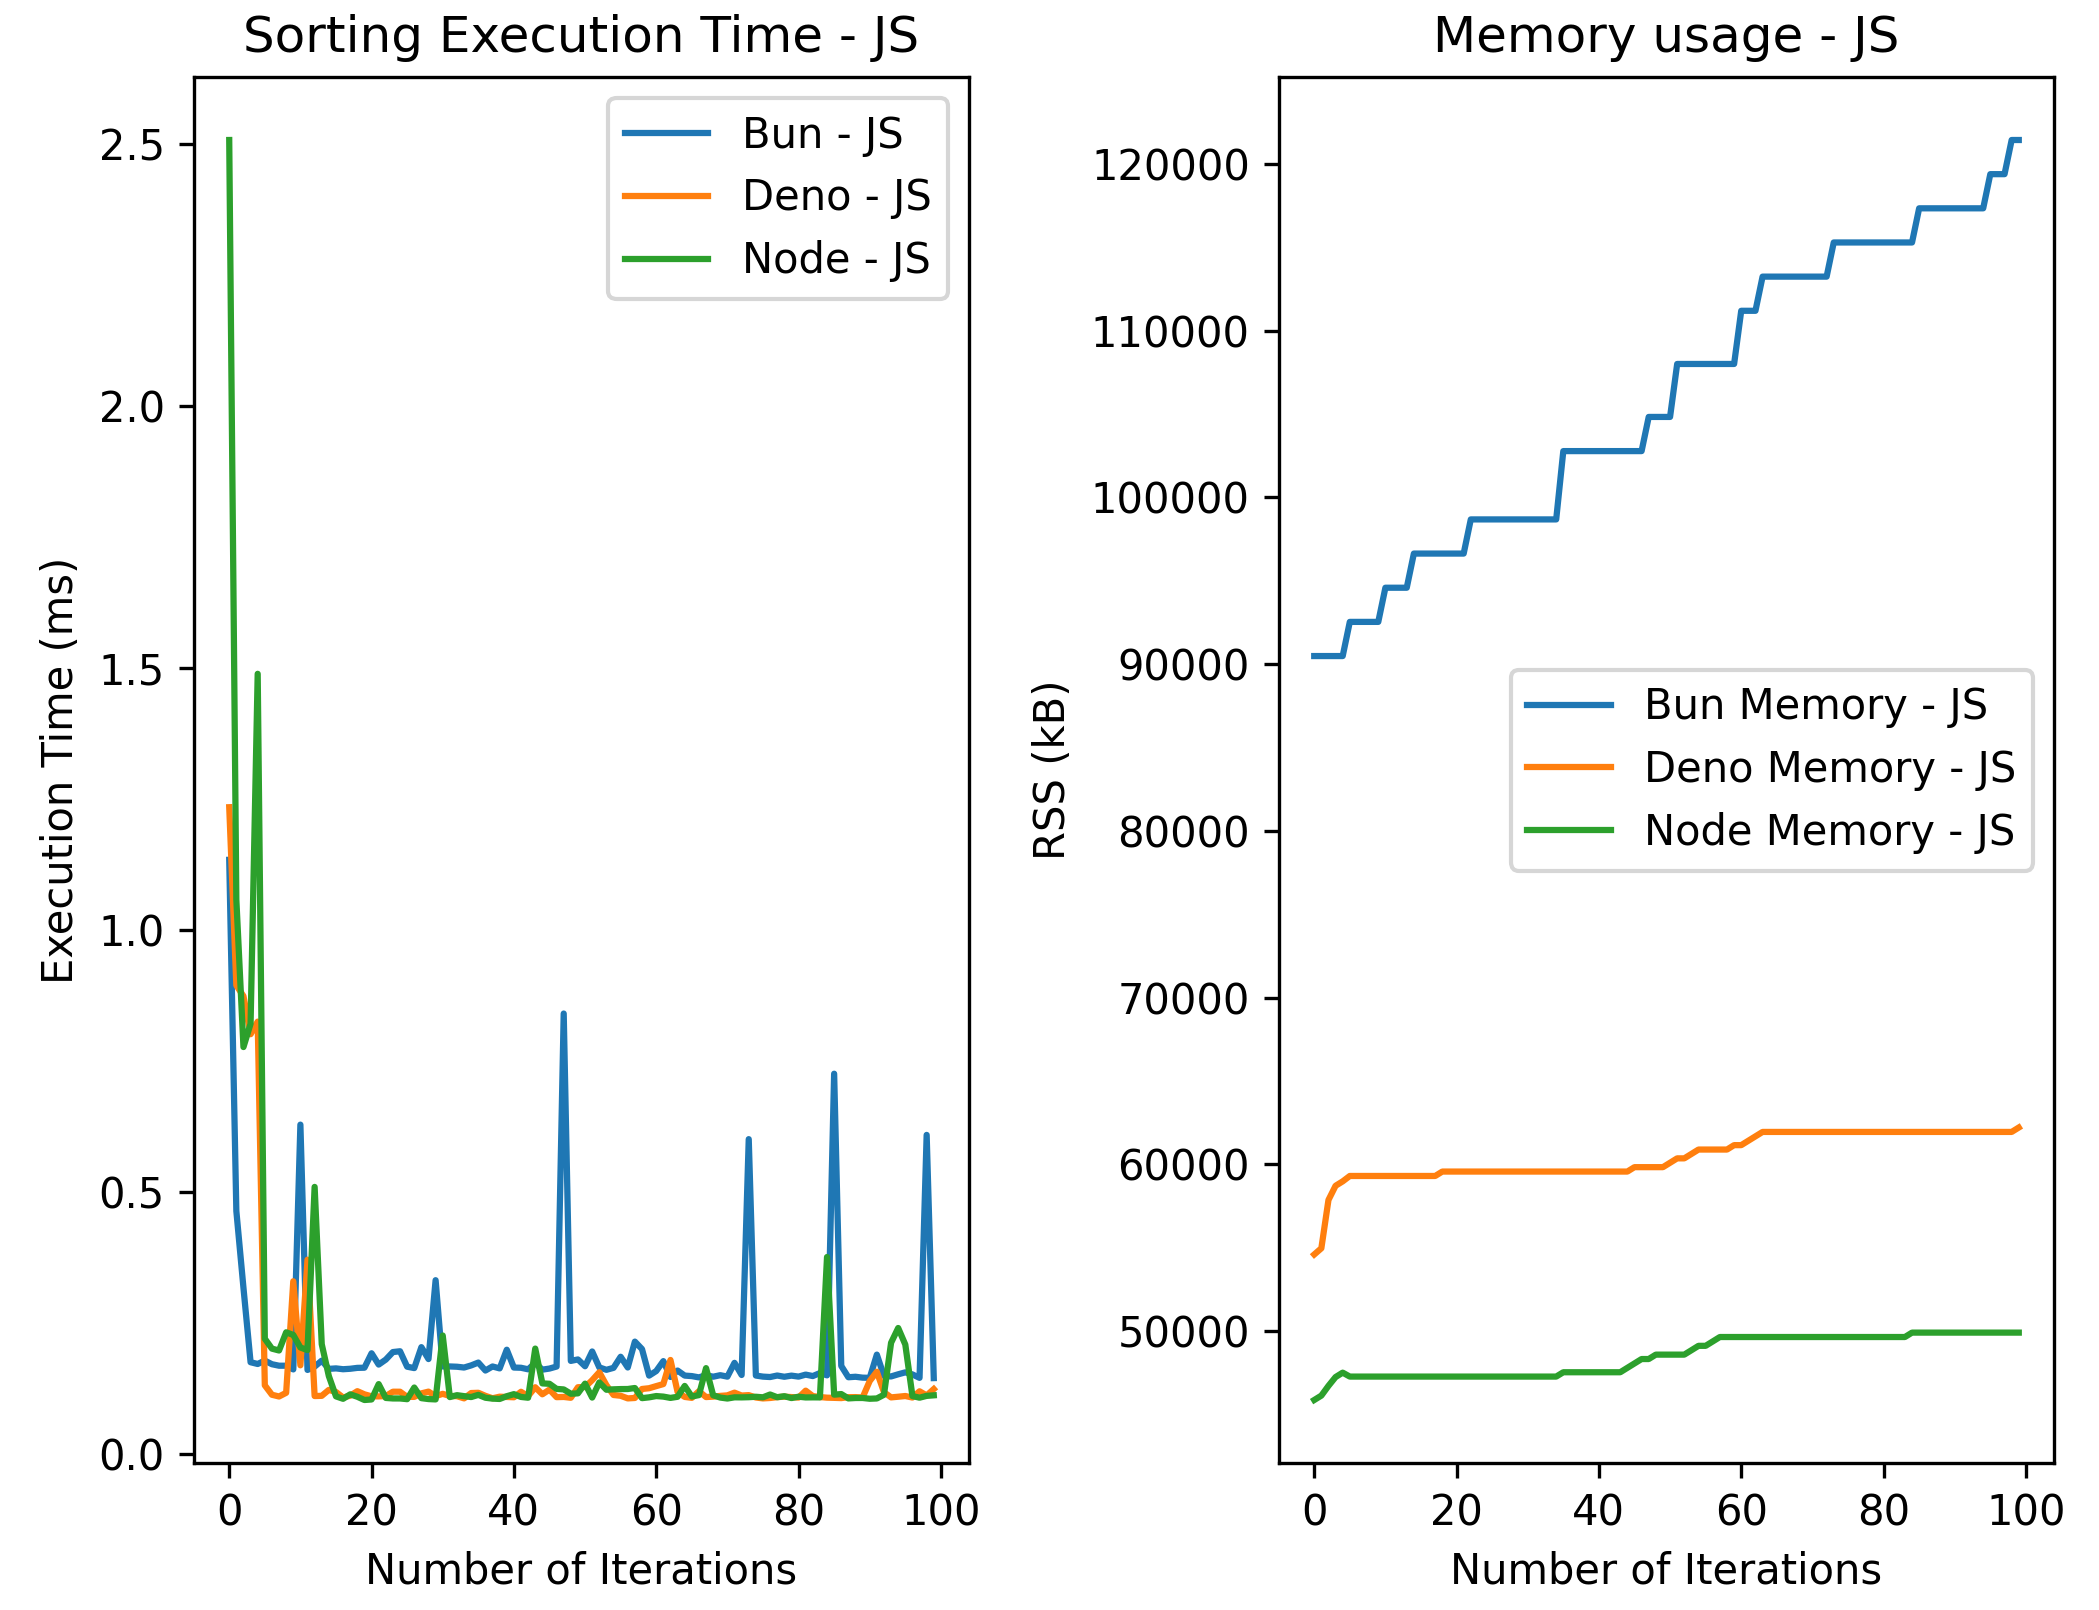
\includegraphics[width=0.68\textwidth]{Figures/sorting/sorting_radix_100_1000_js.png}
  \caption{Wyniki eksperymentów dla algorytmu sortowania pozycyjnego dla 100 iteracji i 1000 elementów - po lewej czas wykonania jednorazowego testu w milisekundach, po prawej ilość zajmowanej pamięci w kilobajtach (kB)}
  \label{fig:radix_sorting_e1}
\end{figure}

Na rysunku \ref{fig:radix_sorting_e1_ts} przedstawiono wyniki eksperymentów dla algorytmu sortowania pozycyjnego dla 100 iteracji i 1000 elementów napisanego w języku TypeScript. Na wykresie przedstawiono czas wykonania jednorazowego testu w milisekundach oraz ilość zajmowanej pamięci w kilobajtach (kB).

\begin{figure}[H]
  \centering
  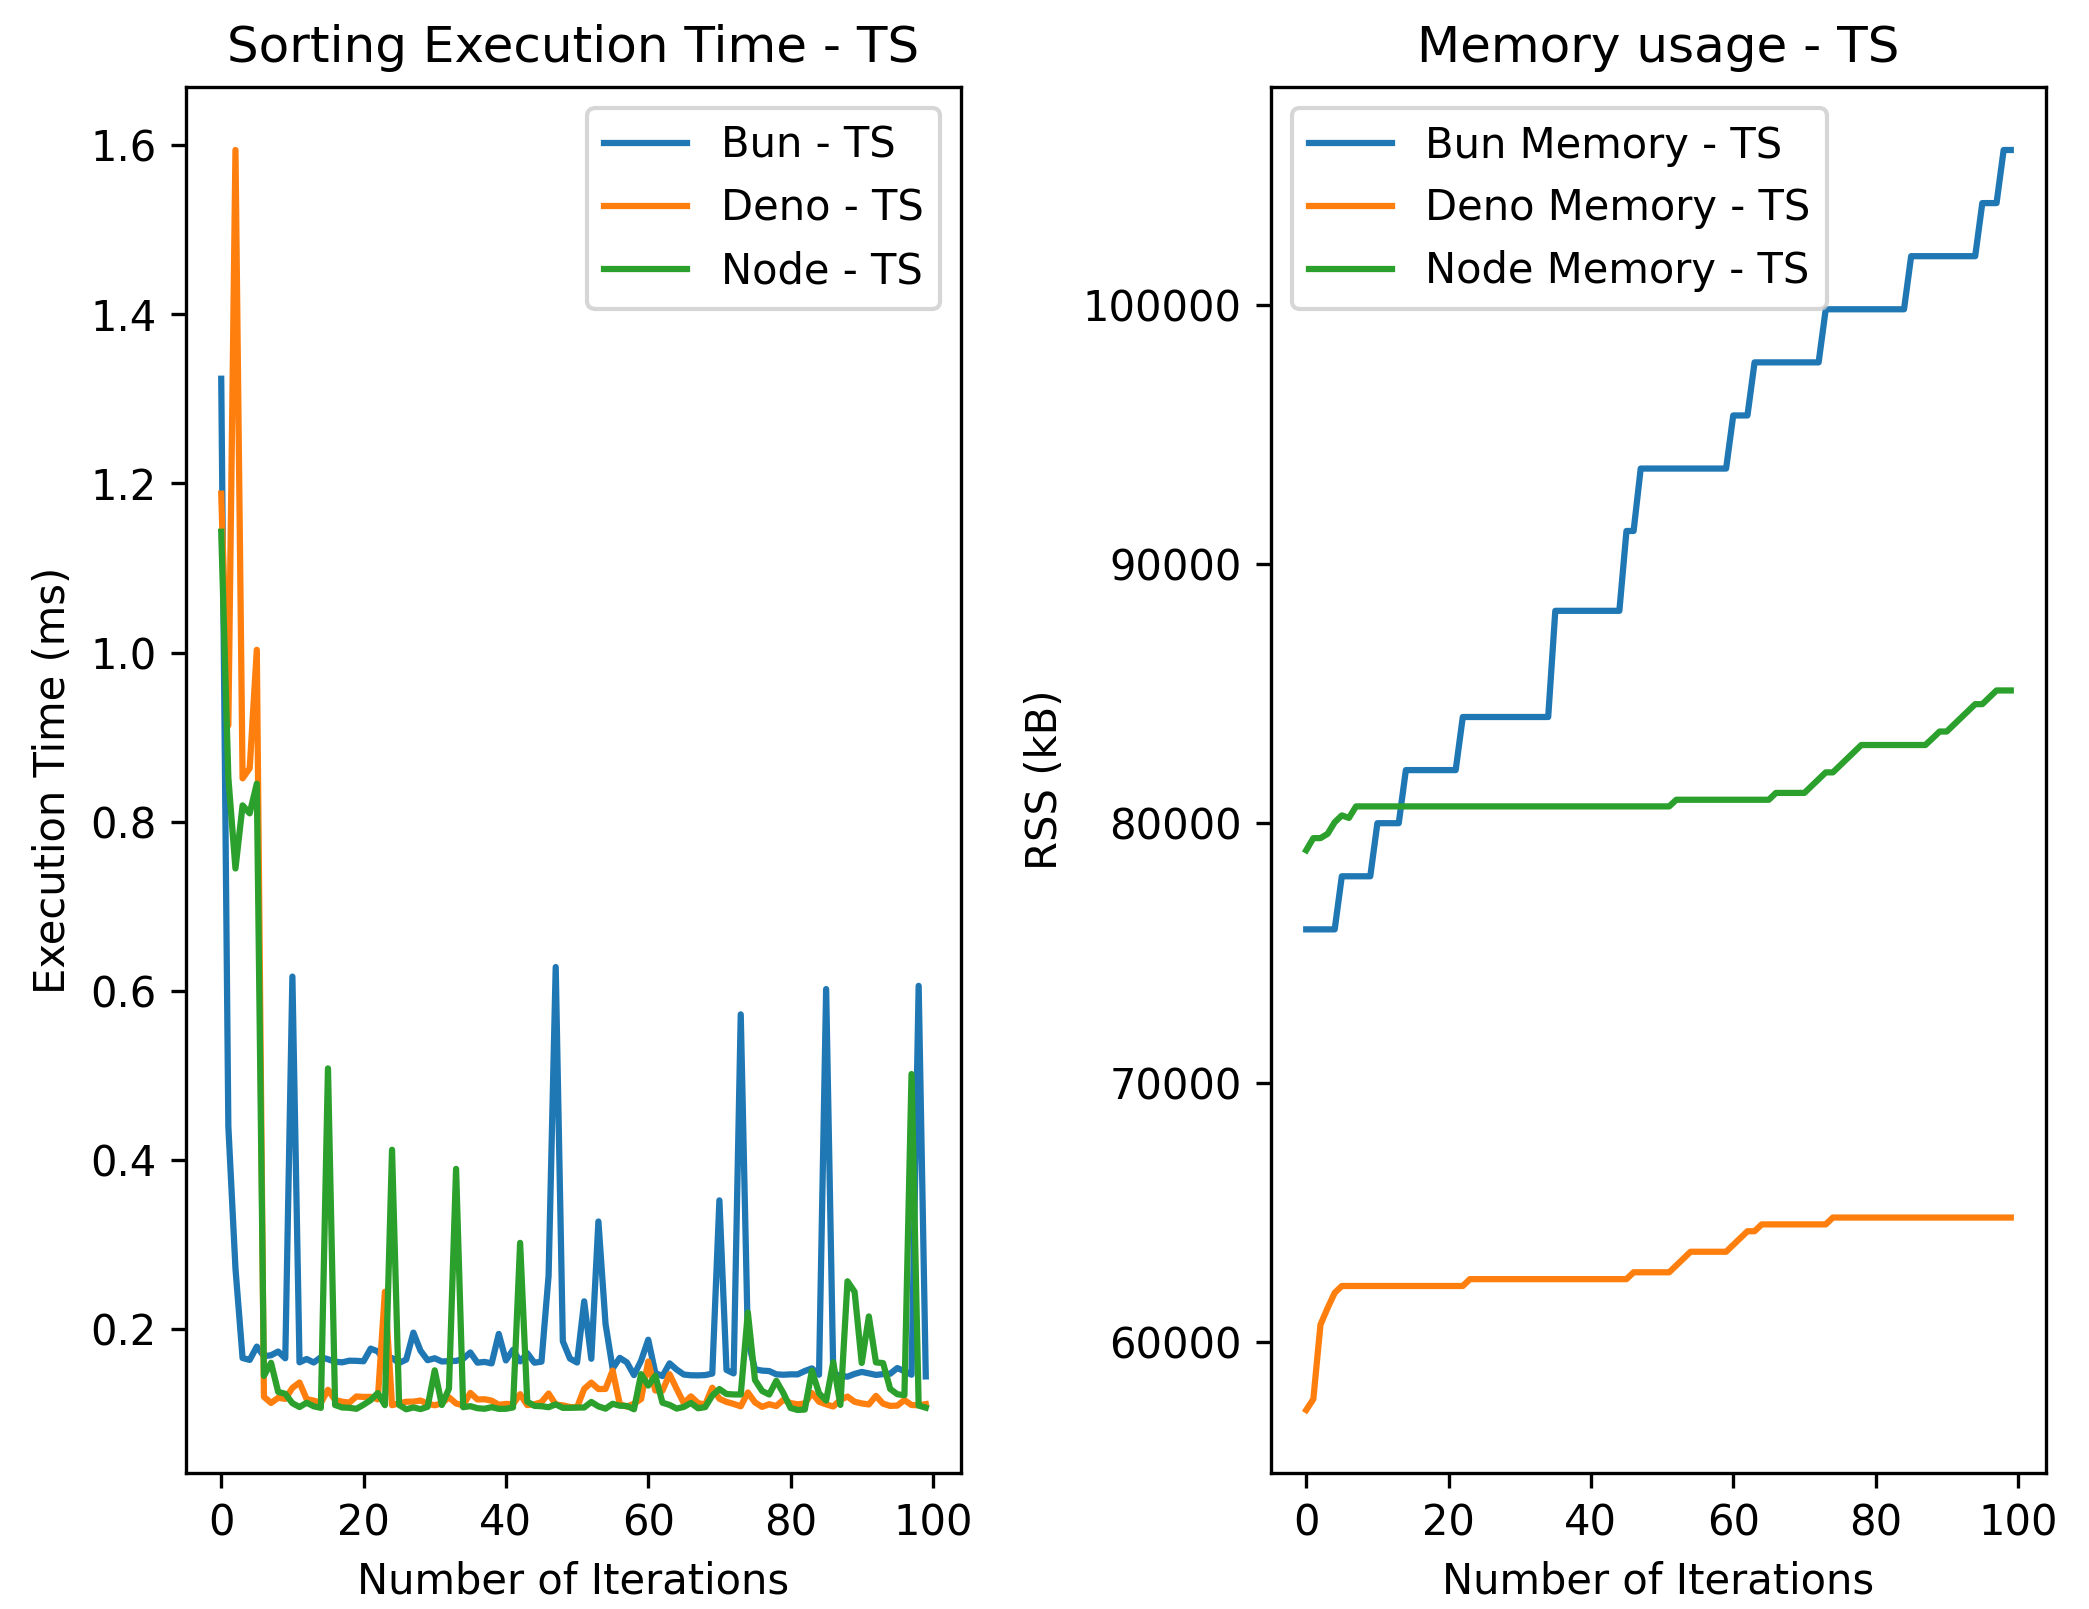
\includegraphics[width=0.68\textwidth]{Figures/sorting/sorting_radix_100_1000_ts.png}
  \caption{Wyniki eksperymentów dla algorytmu sortowania pozycyjnego dla 100 iteracji i 1000 elementów - po lewej czas wykonania jednorazowego testu w milisekundach, po prawej ilość zajmowanej pamięci w kilobajtach (kB)}
  \label{fig:radix_sorting_e1_ts}
\end{figure}

Na rysunku \ref{fig:radix_sorting_e2} przedstawiono wyniki eksperymentów dla algorytmu sortowania pozycyjnego dla 100 iteracji i 1000 elementów napisanego w języku JavaScript. Na wykresie przedstawiono czas wykonania jednorazowego testu w milisekundach oraz ilość zajmowanej pamięci w kilobajtach (kB).

\begin{figure}[H]
  \centering
  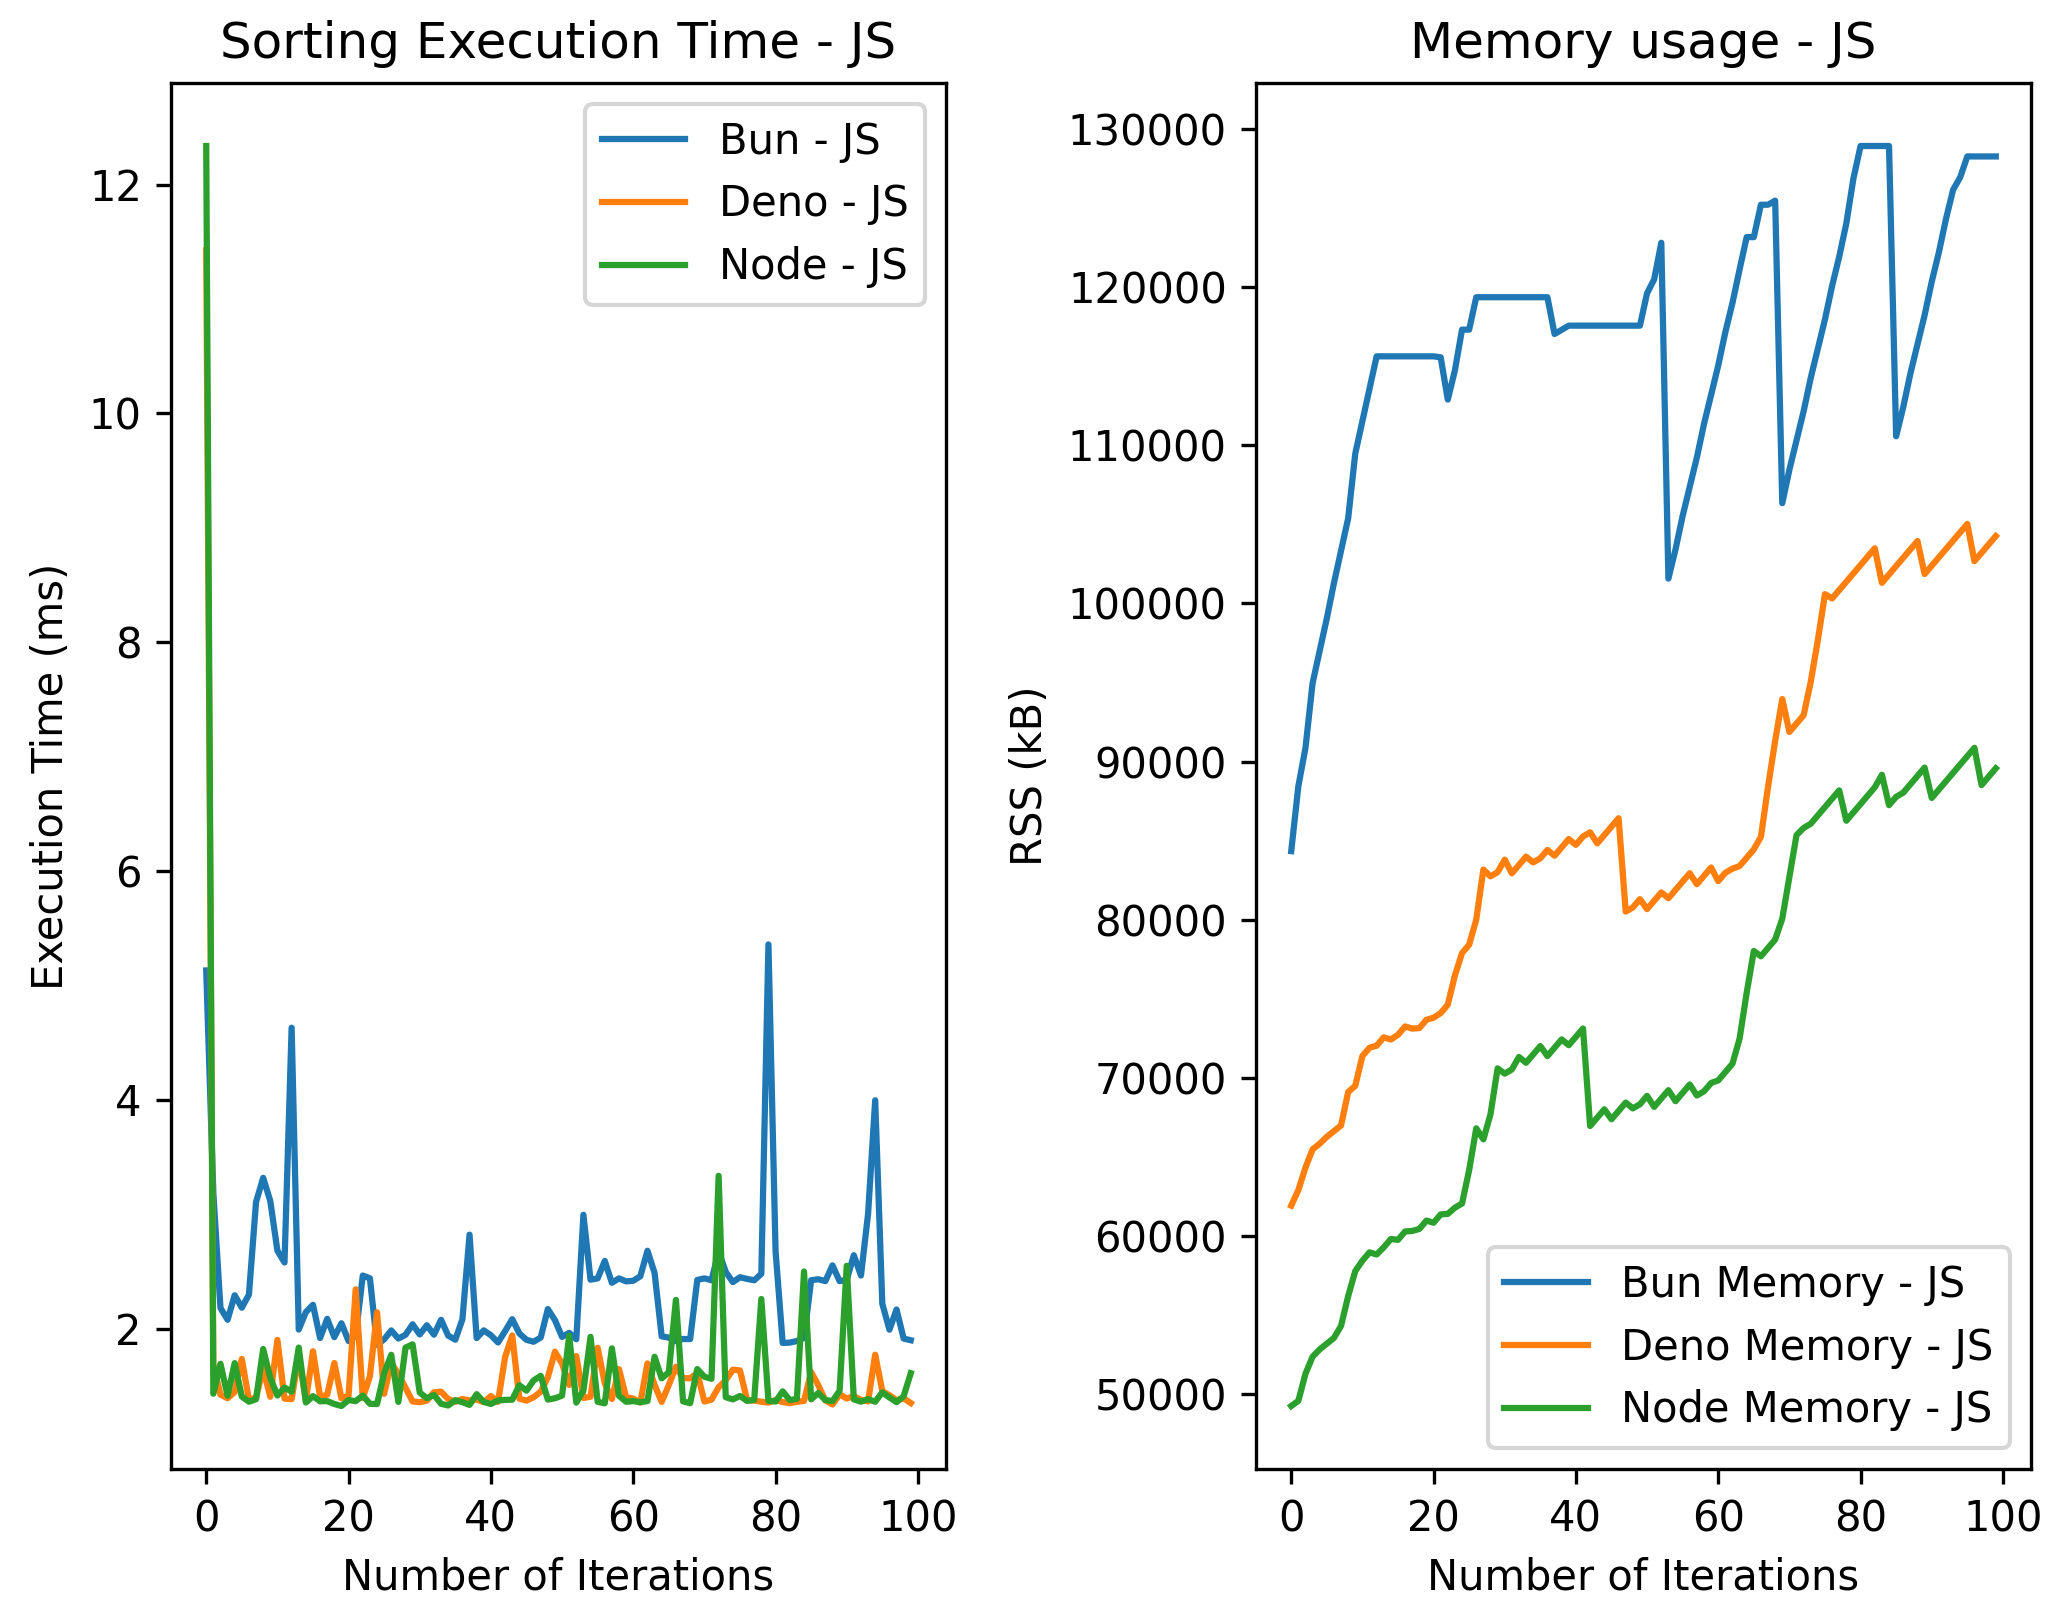
\includegraphics[width=0.68\textwidth]{Figures/sorting/sorting_radix_100_10000_js.png}
  \caption{Wyniki eksperymentów dla algorytmu sortowania pozycyjnego dla 100 iteracji i 10000 elementów - po lewej czas wykonania jednorazowego testu w milisekundach, po prawej ilość zajmowanej pamięci w kilobajtach (kB)}
  \label{fig:radix_sorting_e2}
\end{figure}

Na rysunku \ref{fig:radix_sorting_e2_ts} przedstawiono wyniki eksperymentów dla algorytmu sortowania pozycyjnego dla 100 iteracji i 10000 elementów napisanego w języku TypeScript. Na wykresie przedstawiono czas wykonania jednorazowego testu w milisekundach oraz ilość zajmowanej pamięci w kilobajtach (kB).

\begin{figure}[H]
  \centering
  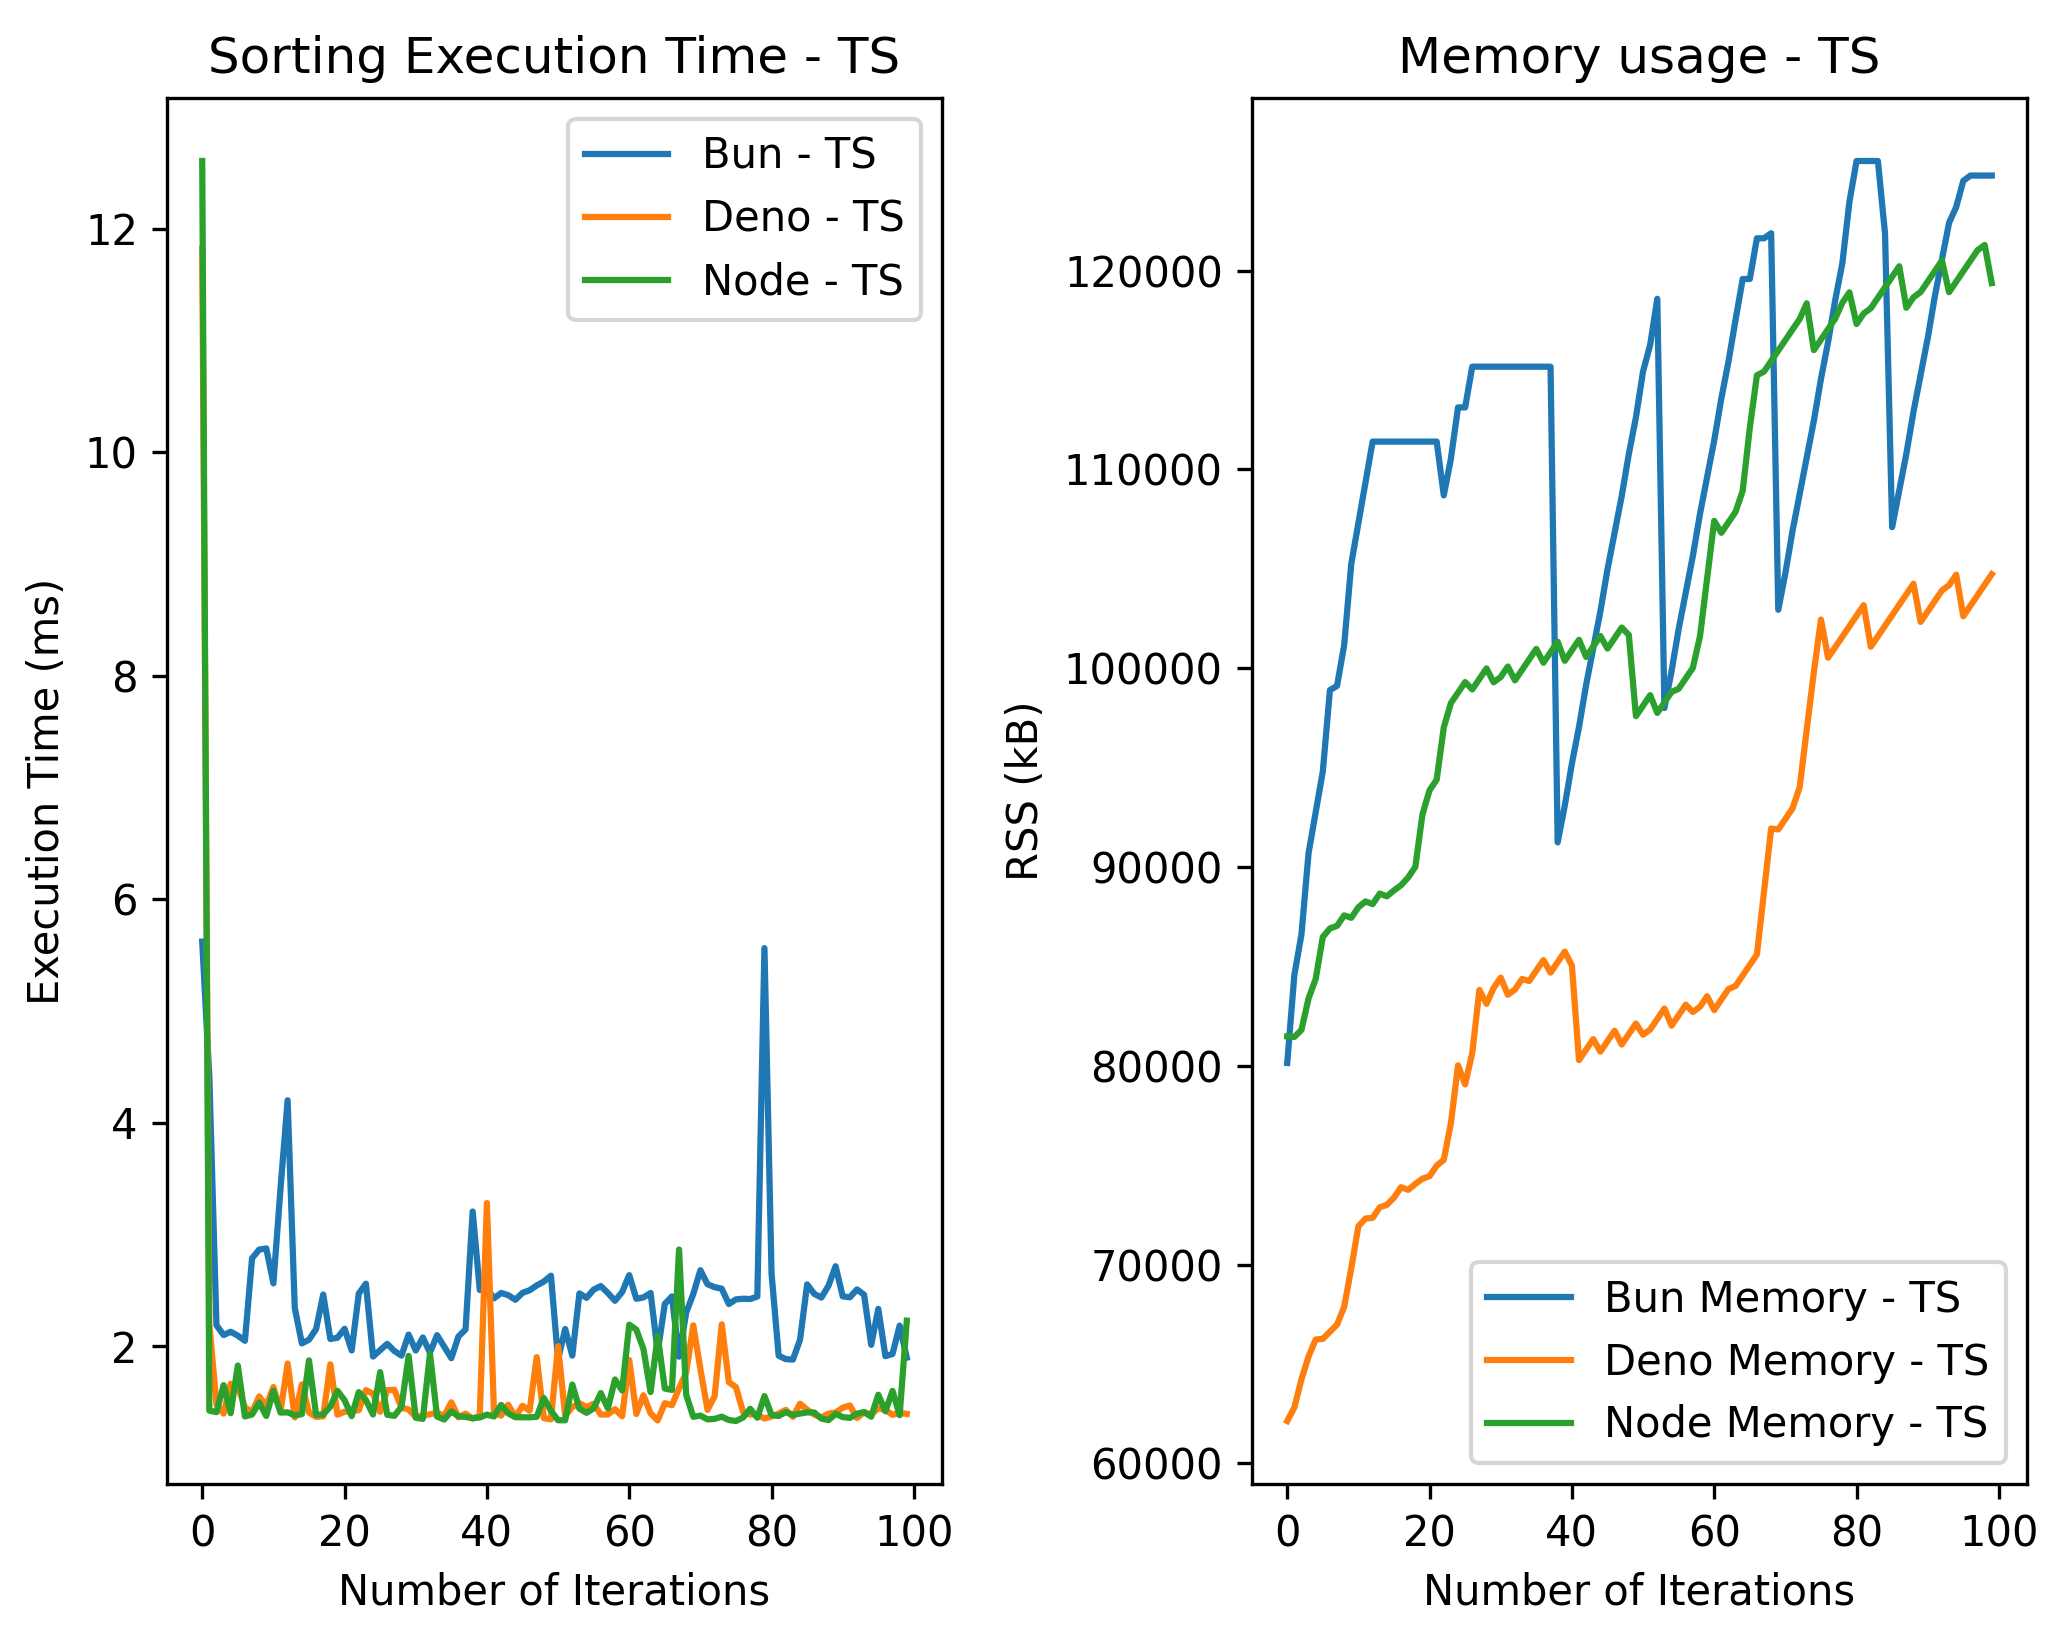
\includegraphics[width=0.68\textwidth]{Figures/sorting/sorting_radix_100_10000_ts.png}
  \caption{Wyniki eksperymentów dla algorytmu sortowania pozycyjnego dla 100 iteracji i 10000 elementów - po lewej czas wykonania jednorazowego testu w milisekundach, po prawej ilość zajmowanej pamięci w kilobajtach (kB)}
  \label{fig:radix_sorting_e2_ts}
\end{figure}

Na rysunku \ref{fig:radix_sorting_e3} przedstawiono wyniki eksperymentów dla algorytmu sortowania  dla 1000 iteracji i 1000 elementów napisanego w języku JavaScript. Na wykresie przedstawiono czas wykonania jednorazowego testu w milisekundach oraz ilość zajmowanej pamięci w kilobajtach (kB).

\begin{figure}[H]
  \centering
  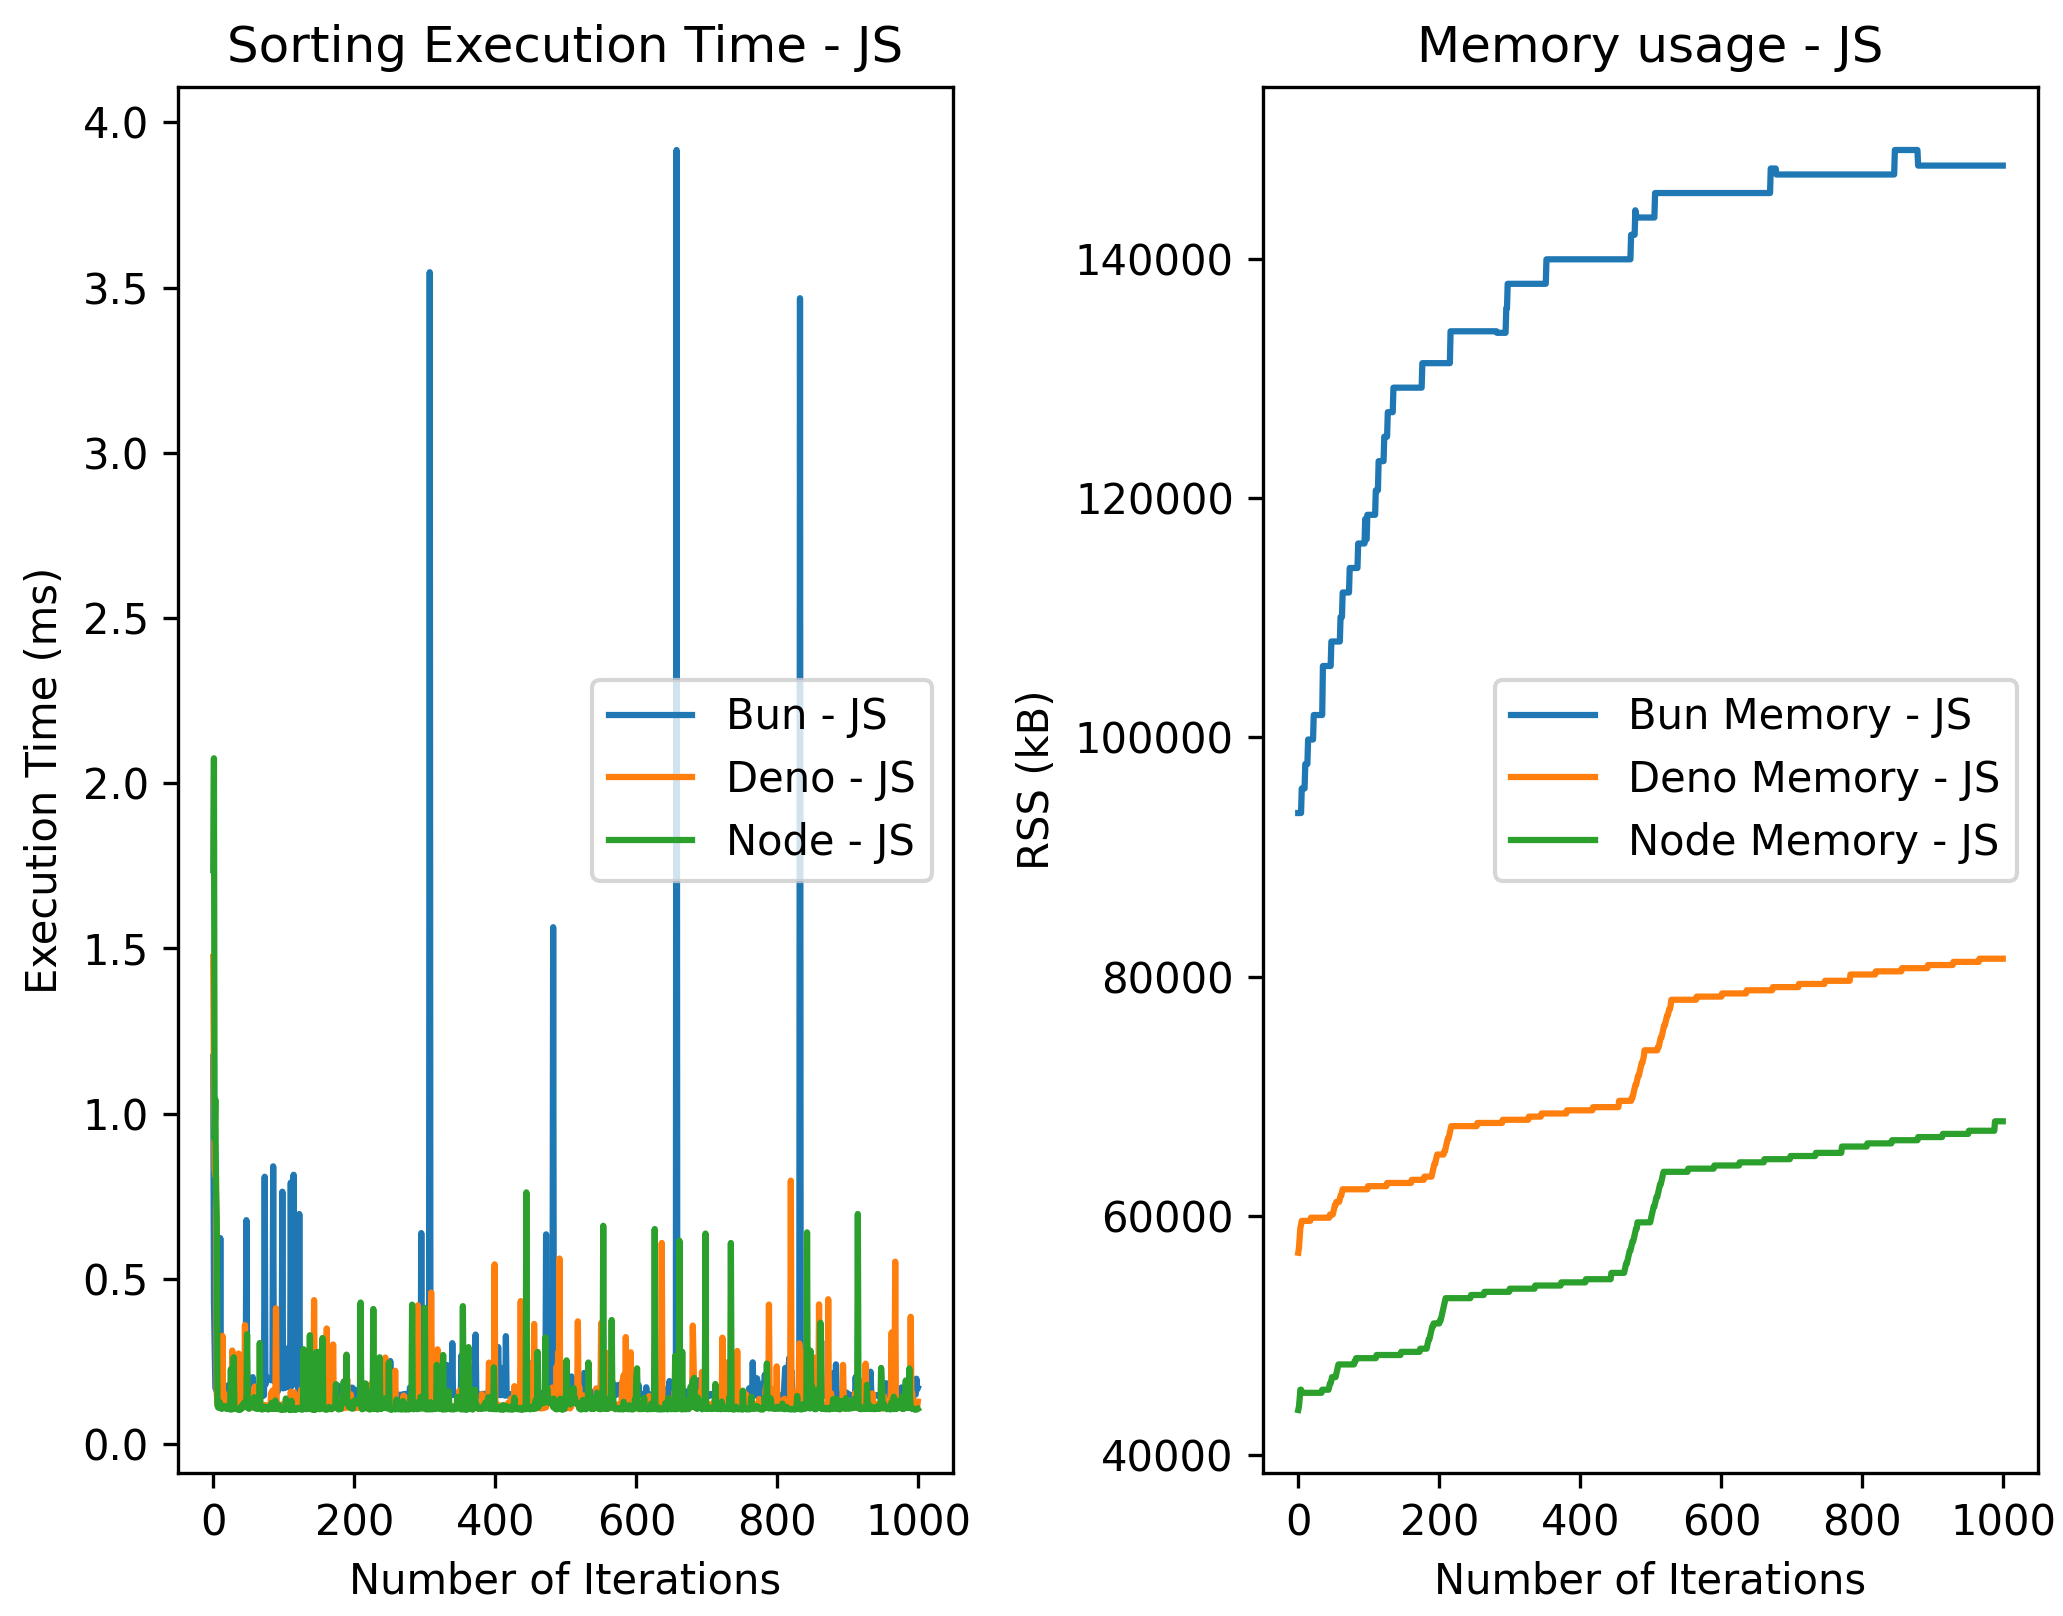
\includegraphics[width=0.68\textwidth]{Figures/sorting/sorting_radix_1000_1000_js.png}
  \caption{Wyniki eksperymentów dla algorytmu sortowania pozycyjnego dla 1000 iteracji i 1000 elementów - po lewej czas wykonania jednorazowego testu w milisekundach, po prawej ilość zajmowanej pamięci w kilobajtach (kB)}
  \label{fig:radix_sorting_e3}
\end{figure}

Na rysunku \ref{fig:radix_sorting_e3_ts} przedstawiono wyniki eksperymentów dla algorytmu sortowania pozycyjnego dla 1000 iteracji i 1000 elementów napisanego w języku TypeScript. Na wykresie przedstawiono czas wykonania jednorazowego testu w milisekundach oraz ilość zajmowanej pamięci w kilobajtach (kB).

\begin{figure}[H]
  \centering
  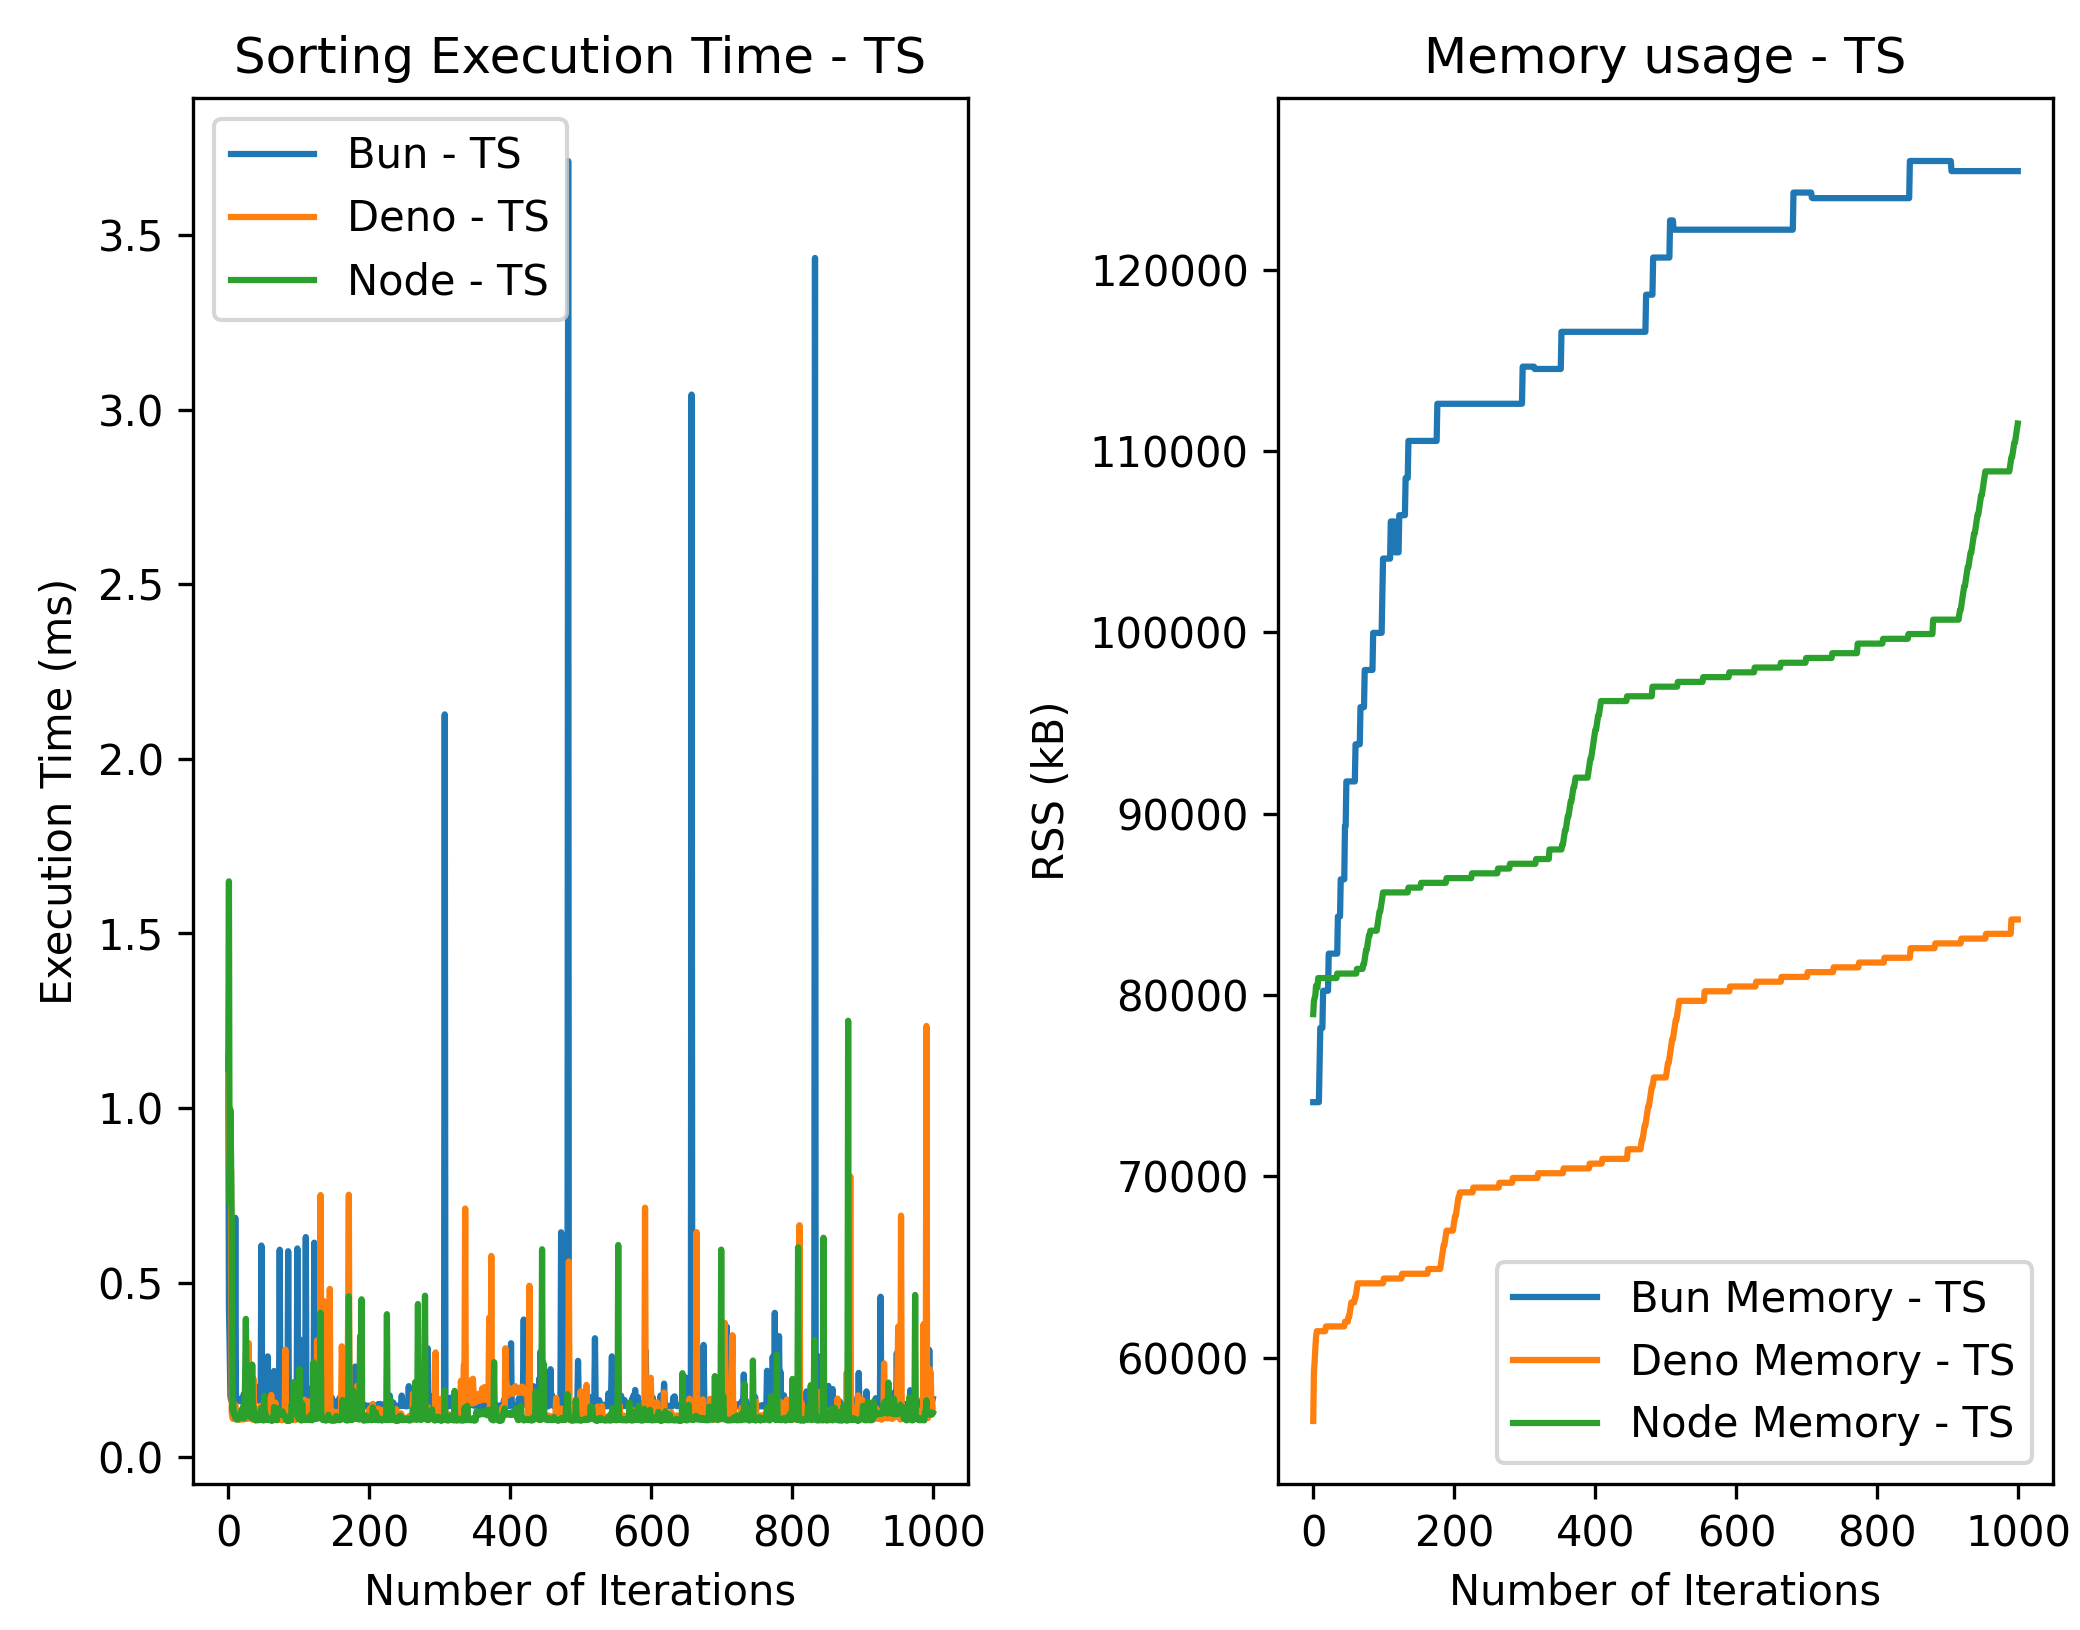
\includegraphics[width=0.68\textwidth]{Figures/sorting/sorting_radix_1000_1000_ts.png}
  \caption{Wyniki eksperymentów dla algorytmu sortowania pozycyjnego dla 1000 iteracji i 1000 elementów - po lewej czas wykonania jednorazowego testu w milisekundach, po prawej ilość zajmowanej pamięci w kilobajtach (kB)}
  \label{fig:radix_sorting_e3_ts}
\end{figure}

Na rysunku \ref{fig:radix_sorting_e4} przedstawiono wyniki eksperymentów dla algorytmu sortowania pozycyjnego dla 100 iteracji i 1000 elementów napisanego w języku JavaScript. Na wykresie przedstawiono czas wykonania jednorazowego testu w milisekundach oraz ilość zajmowanej pamięci w kilobajtach (kB).

\begin{figure}[H]
  \centering
  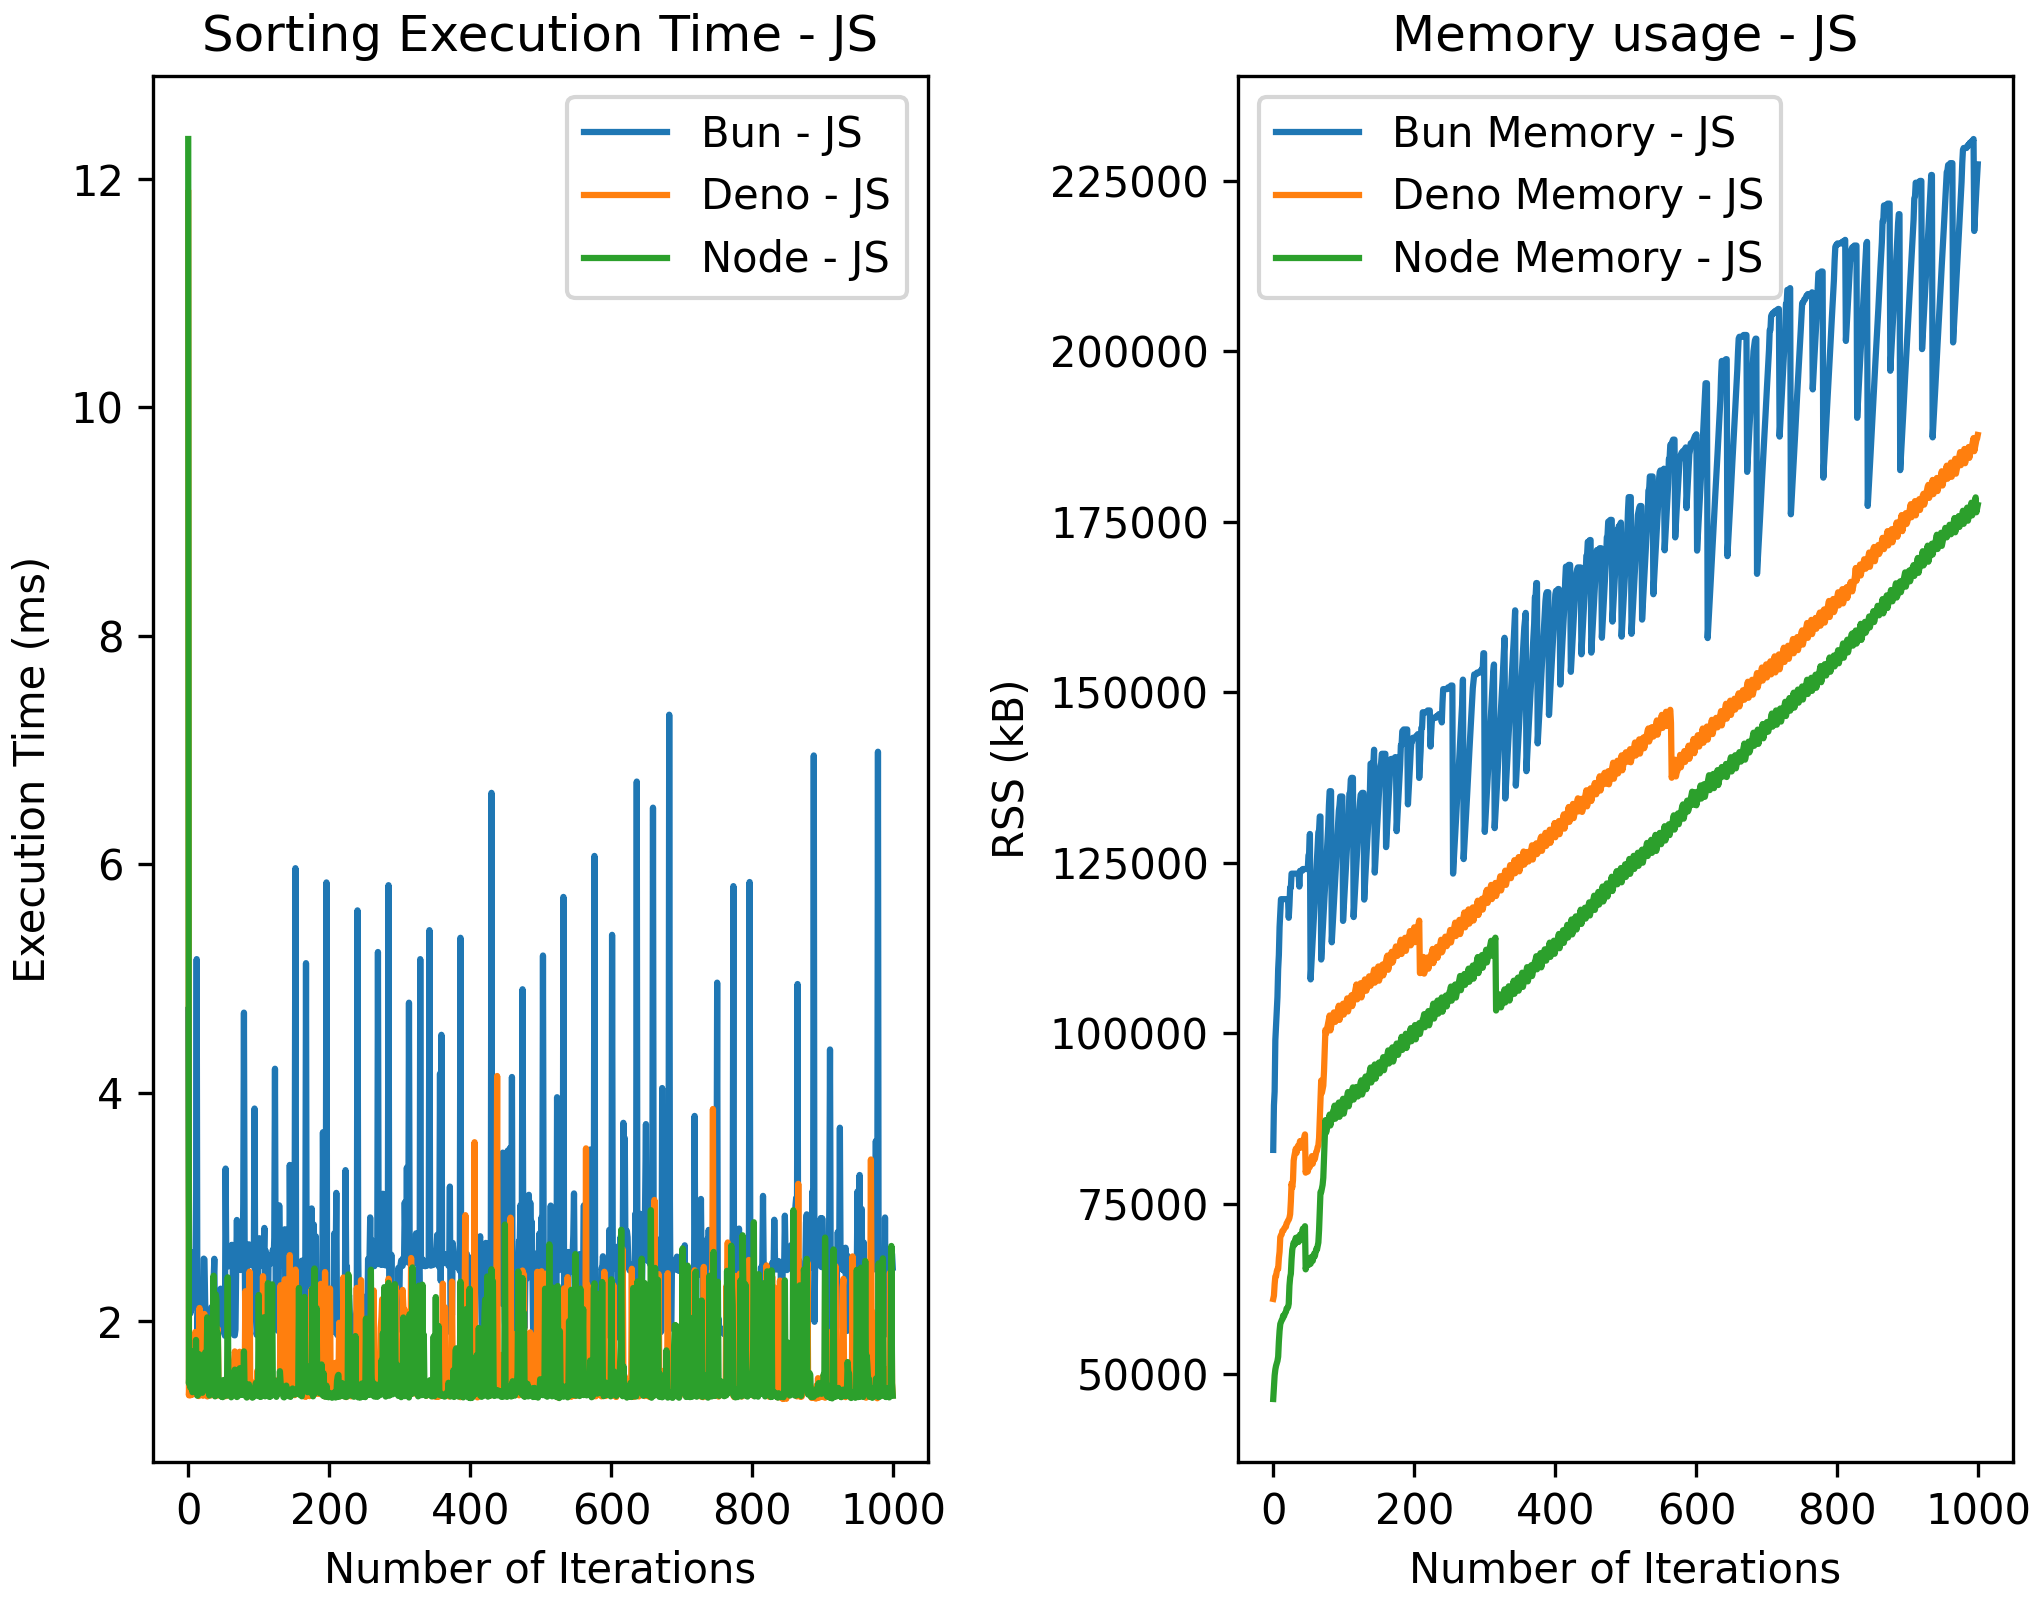
\includegraphics[width=0.68\textwidth]{Figures/sorting/sorting_radix_1000_10000_js.png}
  \caption{Wyniki eksperymentów dla algorytmu sortowania pozycyjnego dla 1000 iteracji i 10000 elementów - po lewej czas wykonania jednorazowego testu w milisekundach, po prawej ilość zajmowanej pamięci w kilobajtach (kB)}
  \label{fig:radix_sorting_e4}
\end{figure}

Na rysunku \ref{fig:radix_sorting_e4_ts} przedstawiono wyniki eksperymentów dla algorytmu sortowania pozycyjnego dla 1000 iteracji i 10000 elementów napisanego w języku TypeScript. Na wykresie przedstawiono czas wykonania jednorazowego testu w milisekundach oraz ilość zajmowanej pamięci w kilobajtach (kB).

\begin{figure}[H]
  \centering
  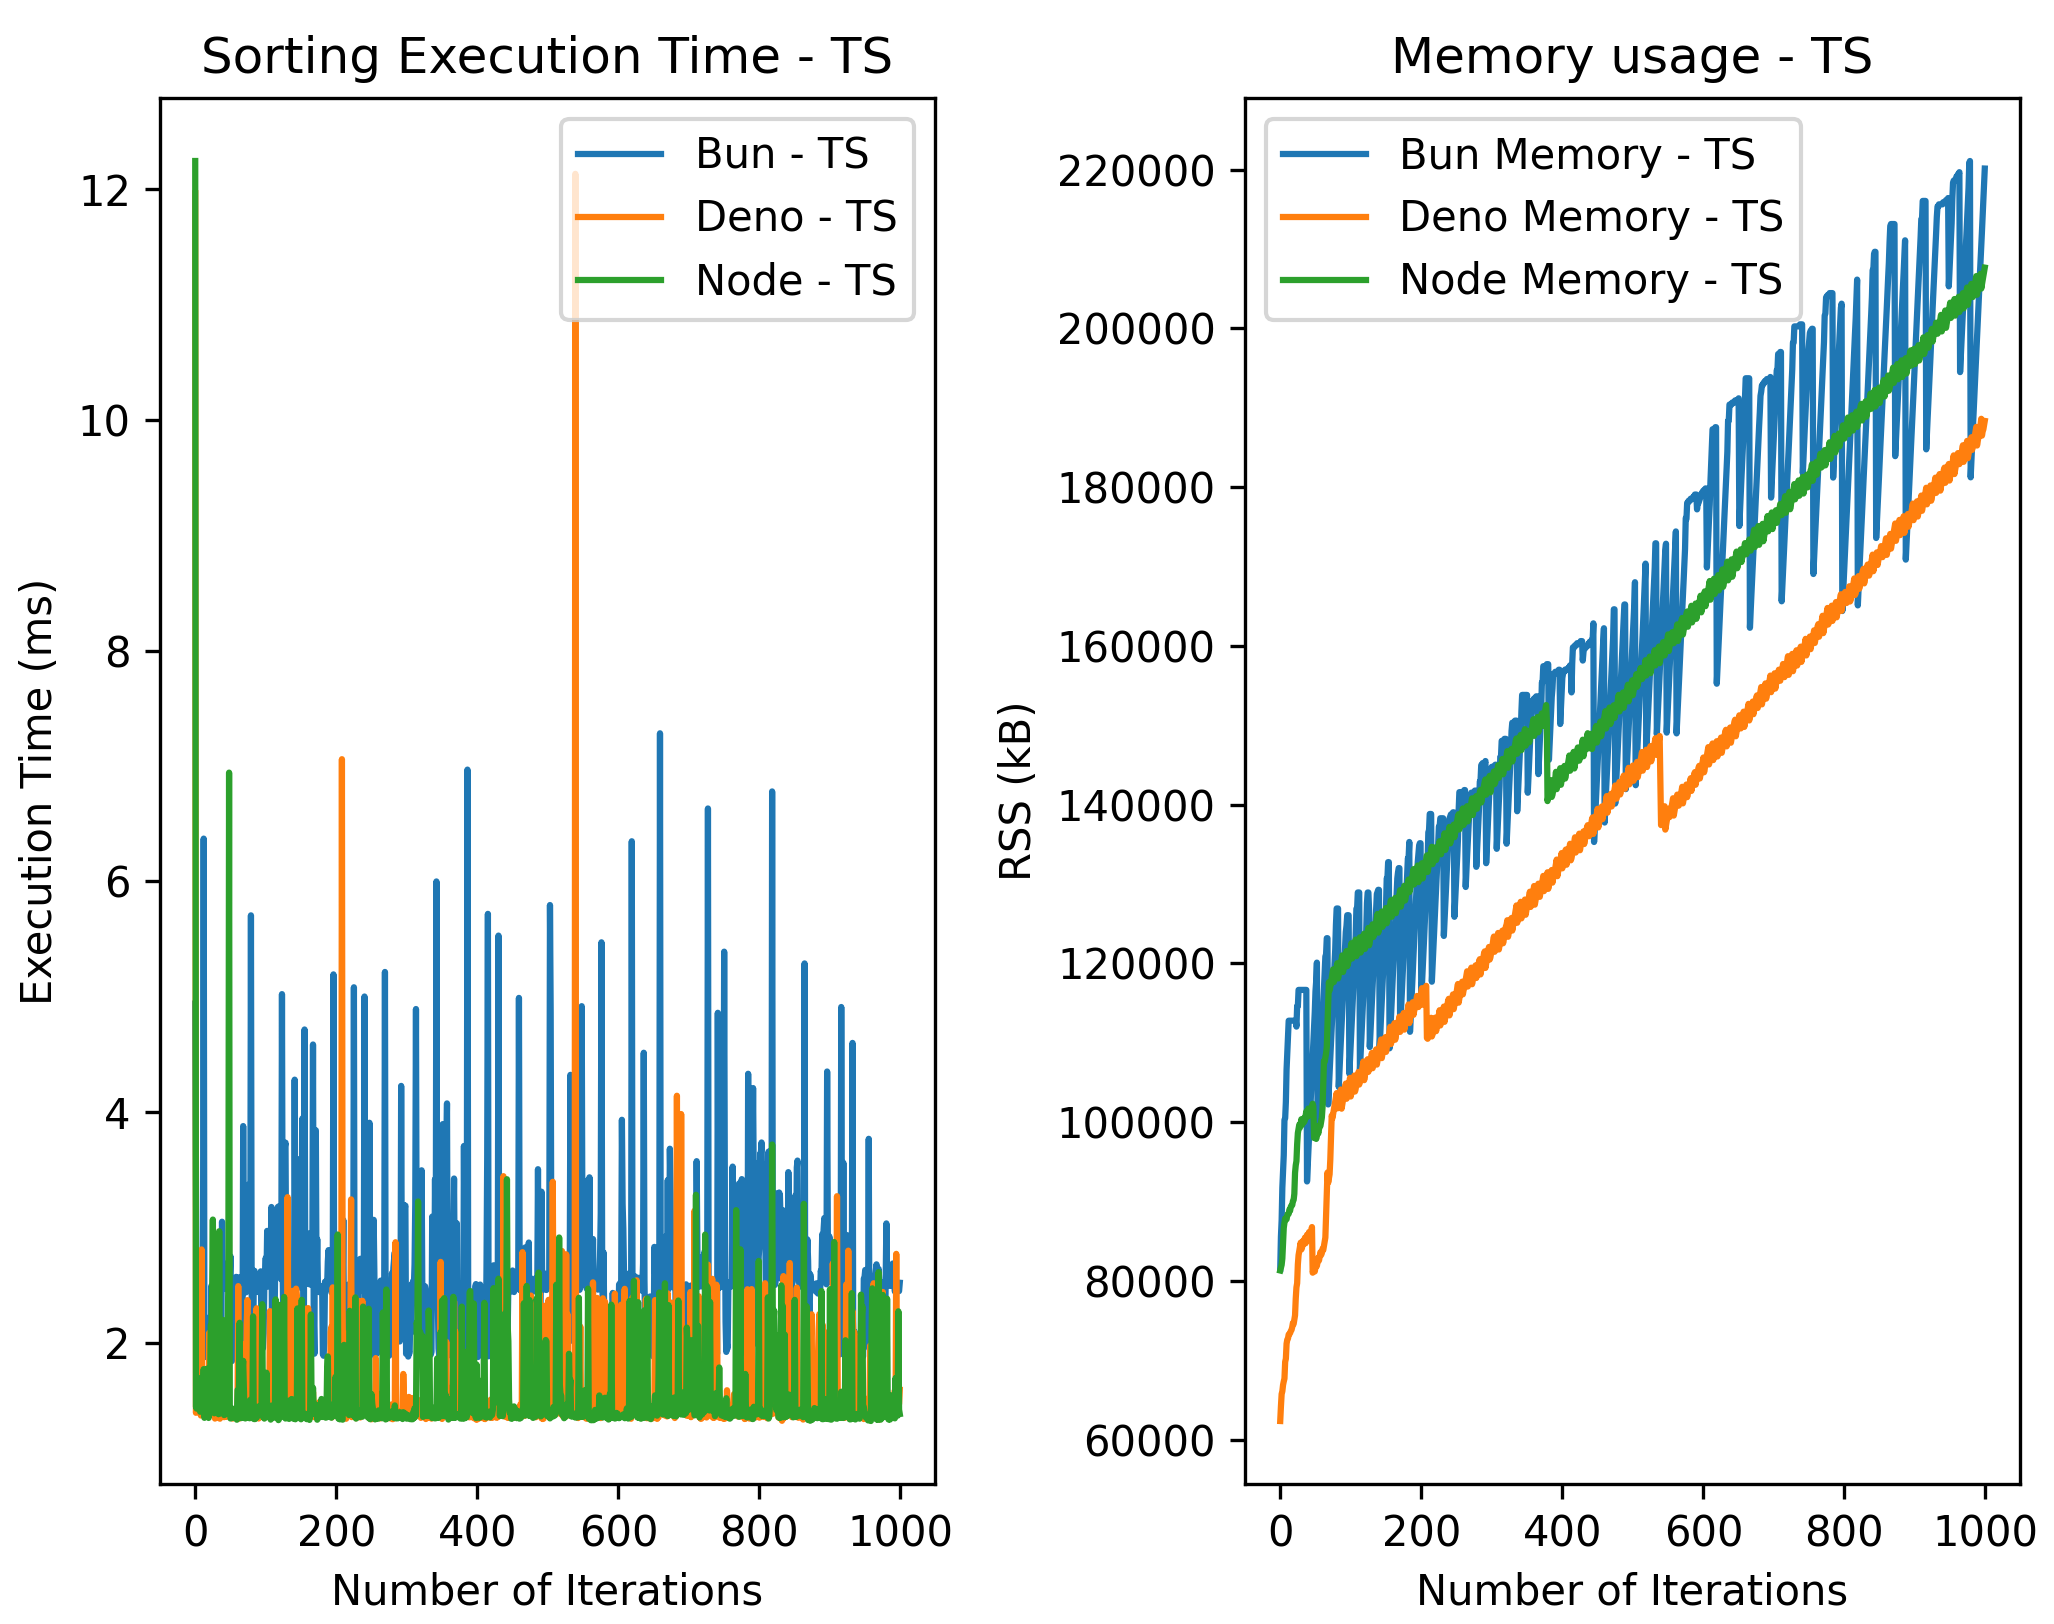
\includegraphics[width=0.68\textwidth]{Figures/sorting/sorting_radix_1000_10000_ts.png}
  \caption{Wyniki eksperymentów dla algorytmu sortowania pozycyjnego dla 100 iteracji i 10000 elementów - po lewej czas wykonania jednorazowego testu w milisekundach, po prawej ilość zajmowanej pamięci w kilobajtach (kB)}
  \label{fig:radix_sorting_e4_ts}
\end{figure}

\subsection{Algorytmy kodowania}
W celu zbadania wydajności możliwości kodowania dla środowisk, użyto algorytmu kodowania \textit{Base64}, który jest najpopularniejszym algorytmem kodowania wykorzystywanym w aplikacjach webowych. W tabeli \ref{tab:encoding_experiments} przedstawiono liczbę przeprowadzonych eksperymentów, długość kodowanego słowa.

\begin{table}[H]
  \centering
  \caption{Parametry eksperymentów algorytmu kodowania \textit{Base64}}
  \begin{tabular}{|c|c|}
    \hline
    \textbf{Liczba eksperymentów} & \textbf{Długość słowa}\\ \hline
    1000 & 8192 \\ \hline
    100 & 32768 \\ \hline
  \end{tabular}
  \label{tab:encoding_experiments}
\end{table}

\subsubsection{Wyniki}
Na rysunku \ref{fig:encoding_e1_js} przedstawiono wyniki eksperymentów dla operacji kodowania z wykorzystaniem algorytmu kodowania \textit{Base64} dla 100 iteracji i 32768 znaków napisanego w języku JavaScript. Na wykresie przedstawiono czas wykonania jednorazowego testu w milisekundach oraz ilość zajmowanej pamięci w kilobajtach (kB).

\begin{figure}[H]
  \centering
  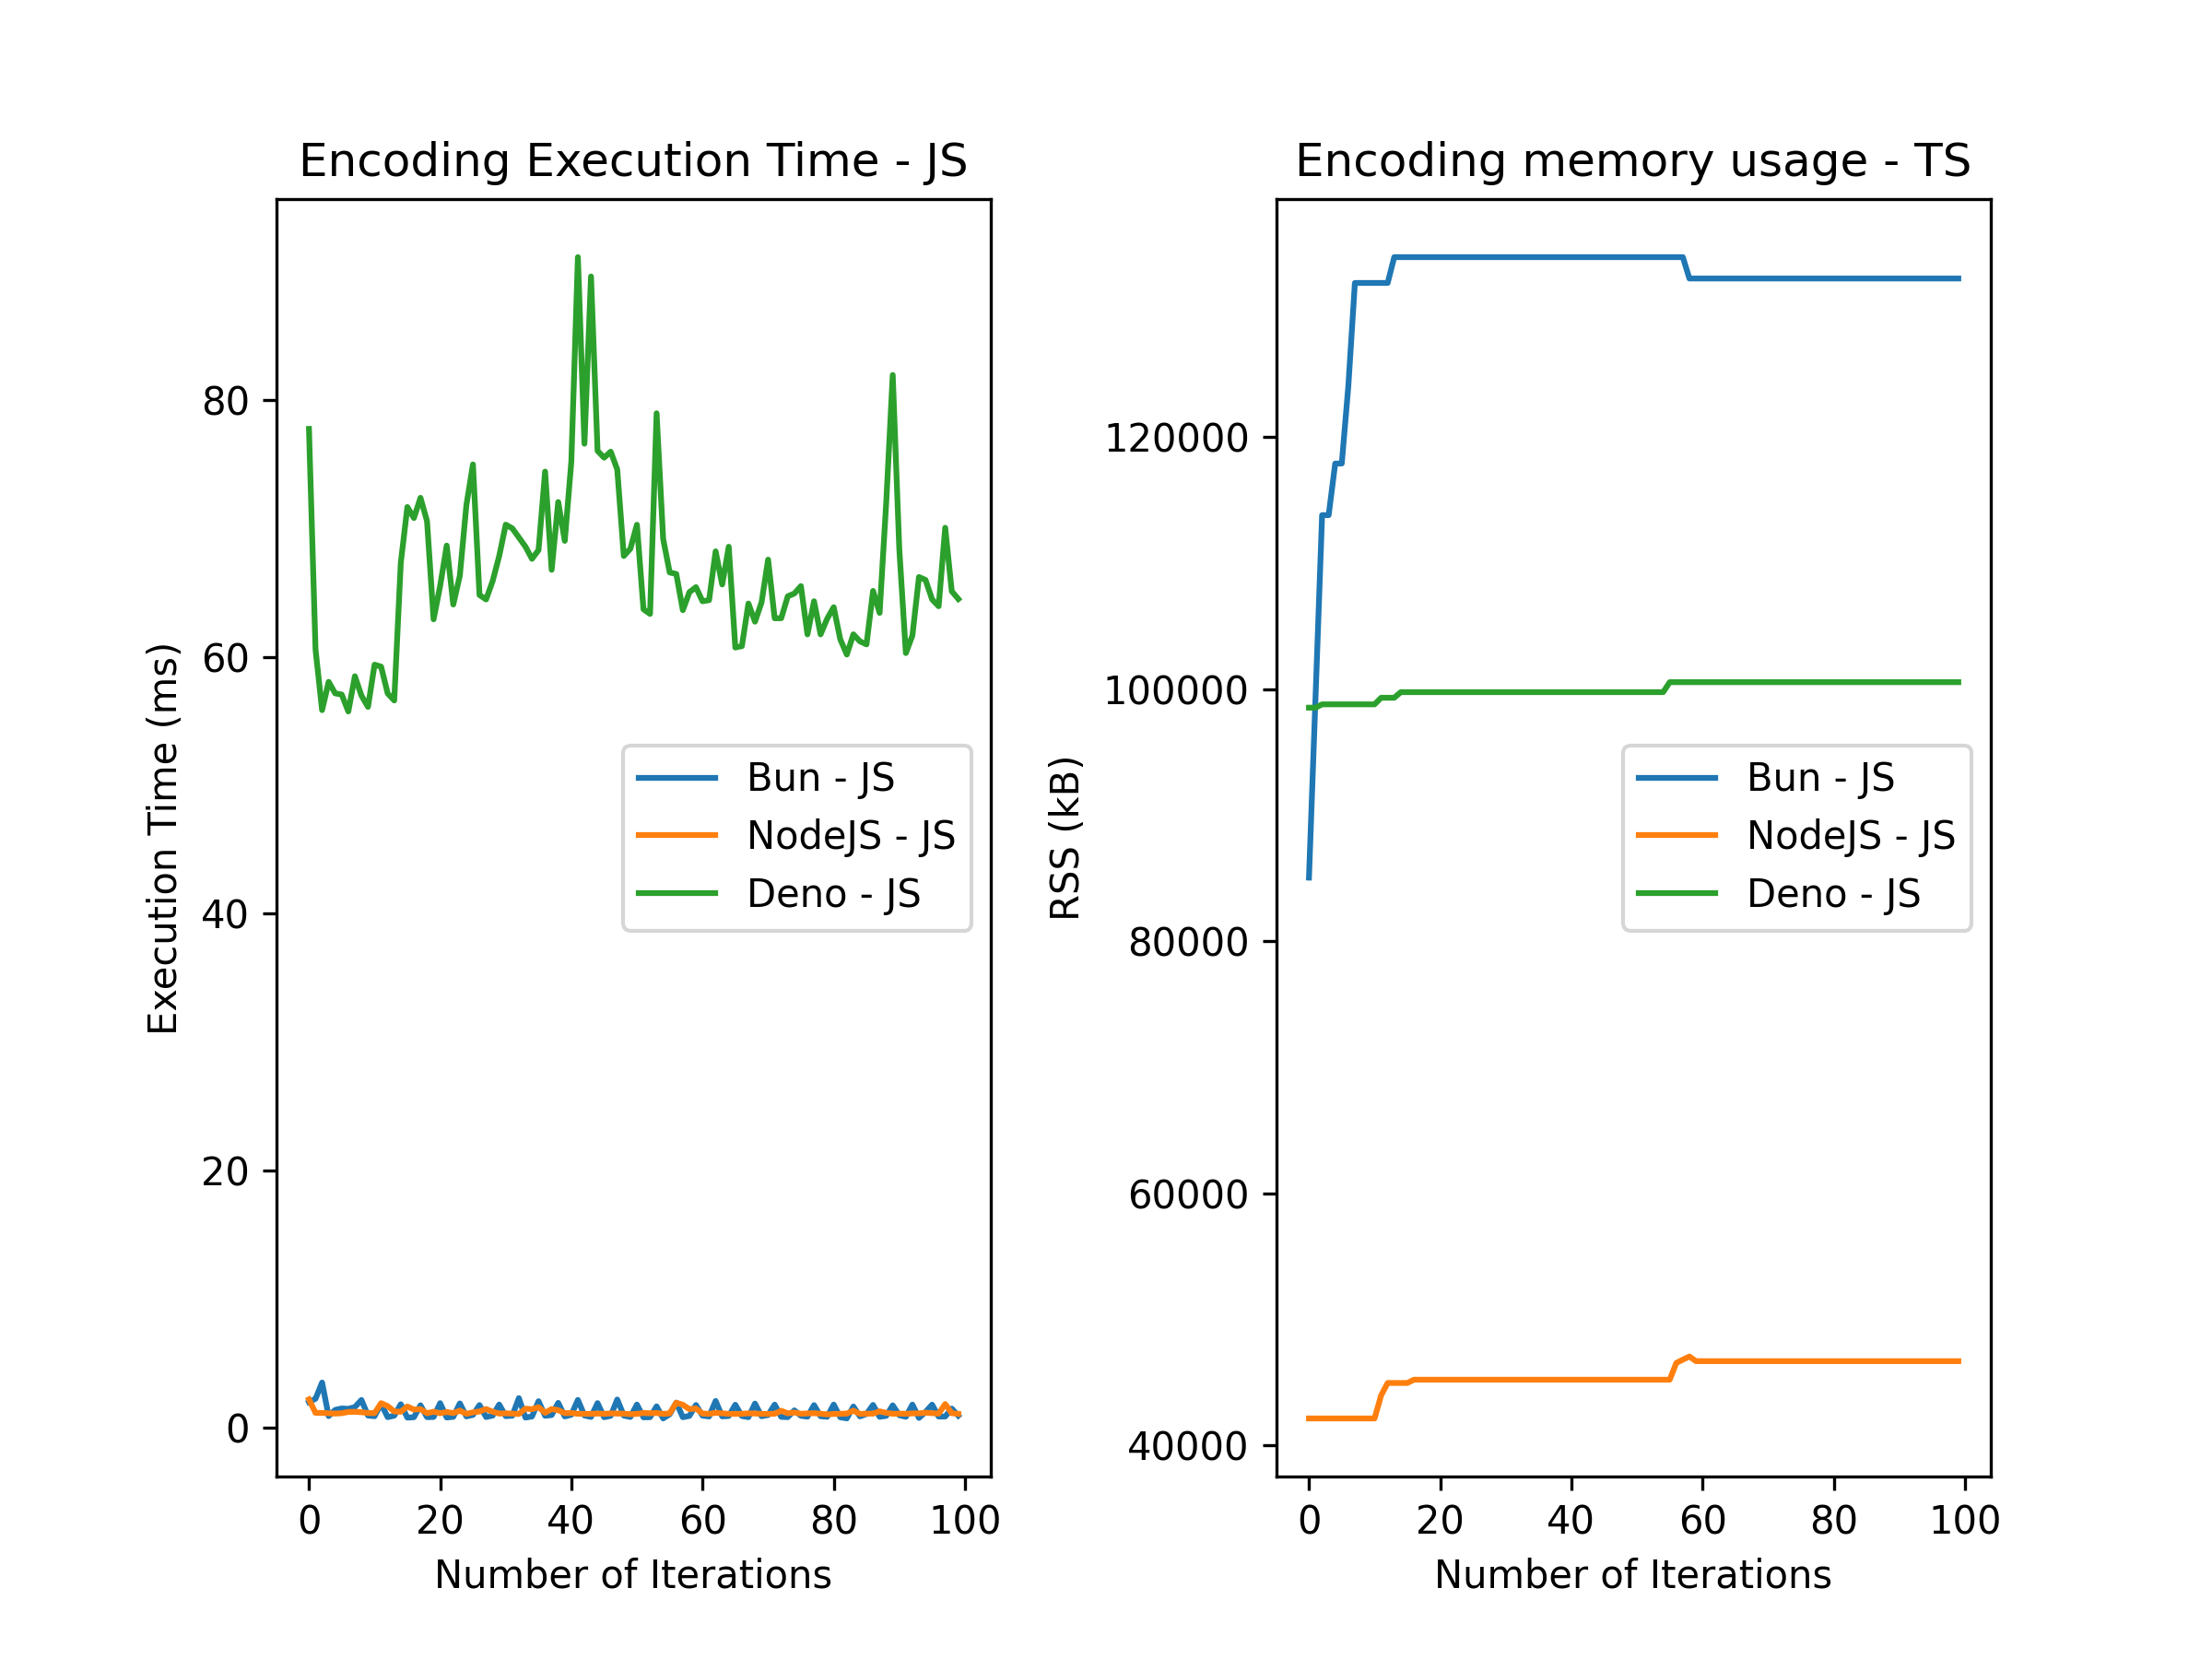
\includegraphics[width=0.68\textwidth]{Figures/coding/base64_100_encoding_js.png}
  \caption{Wyniki eksperymentów dla operacji kodowania z wykorzystaniem algorytmu \textit{Base64} dla 100 iteracji oraz 32768 znaków - po lewej czas wykonania jednorazowego testu w milisekundach, po prawej ilość zajmowanej pamięci w kilobajtach (kB)}
  \label{fig:encoding_e1_js}
\end{figure}

Na rysunku \ref{fig:decoding_e1_js} przedstawiono wyniki eksperymentów dla operacji dekodowania z wykorzystaniem kodowania \textit{Base64} dla 100 iteracji i 32768 znaków napisanego w języku JavaScript. Na wykresie przedstawiono czas wykonania jednorazowego testu w milisekundach oraz ilość zajmowanej pamięci w kilobajtach (kB).

\begin{figure}[H]
  \centering
  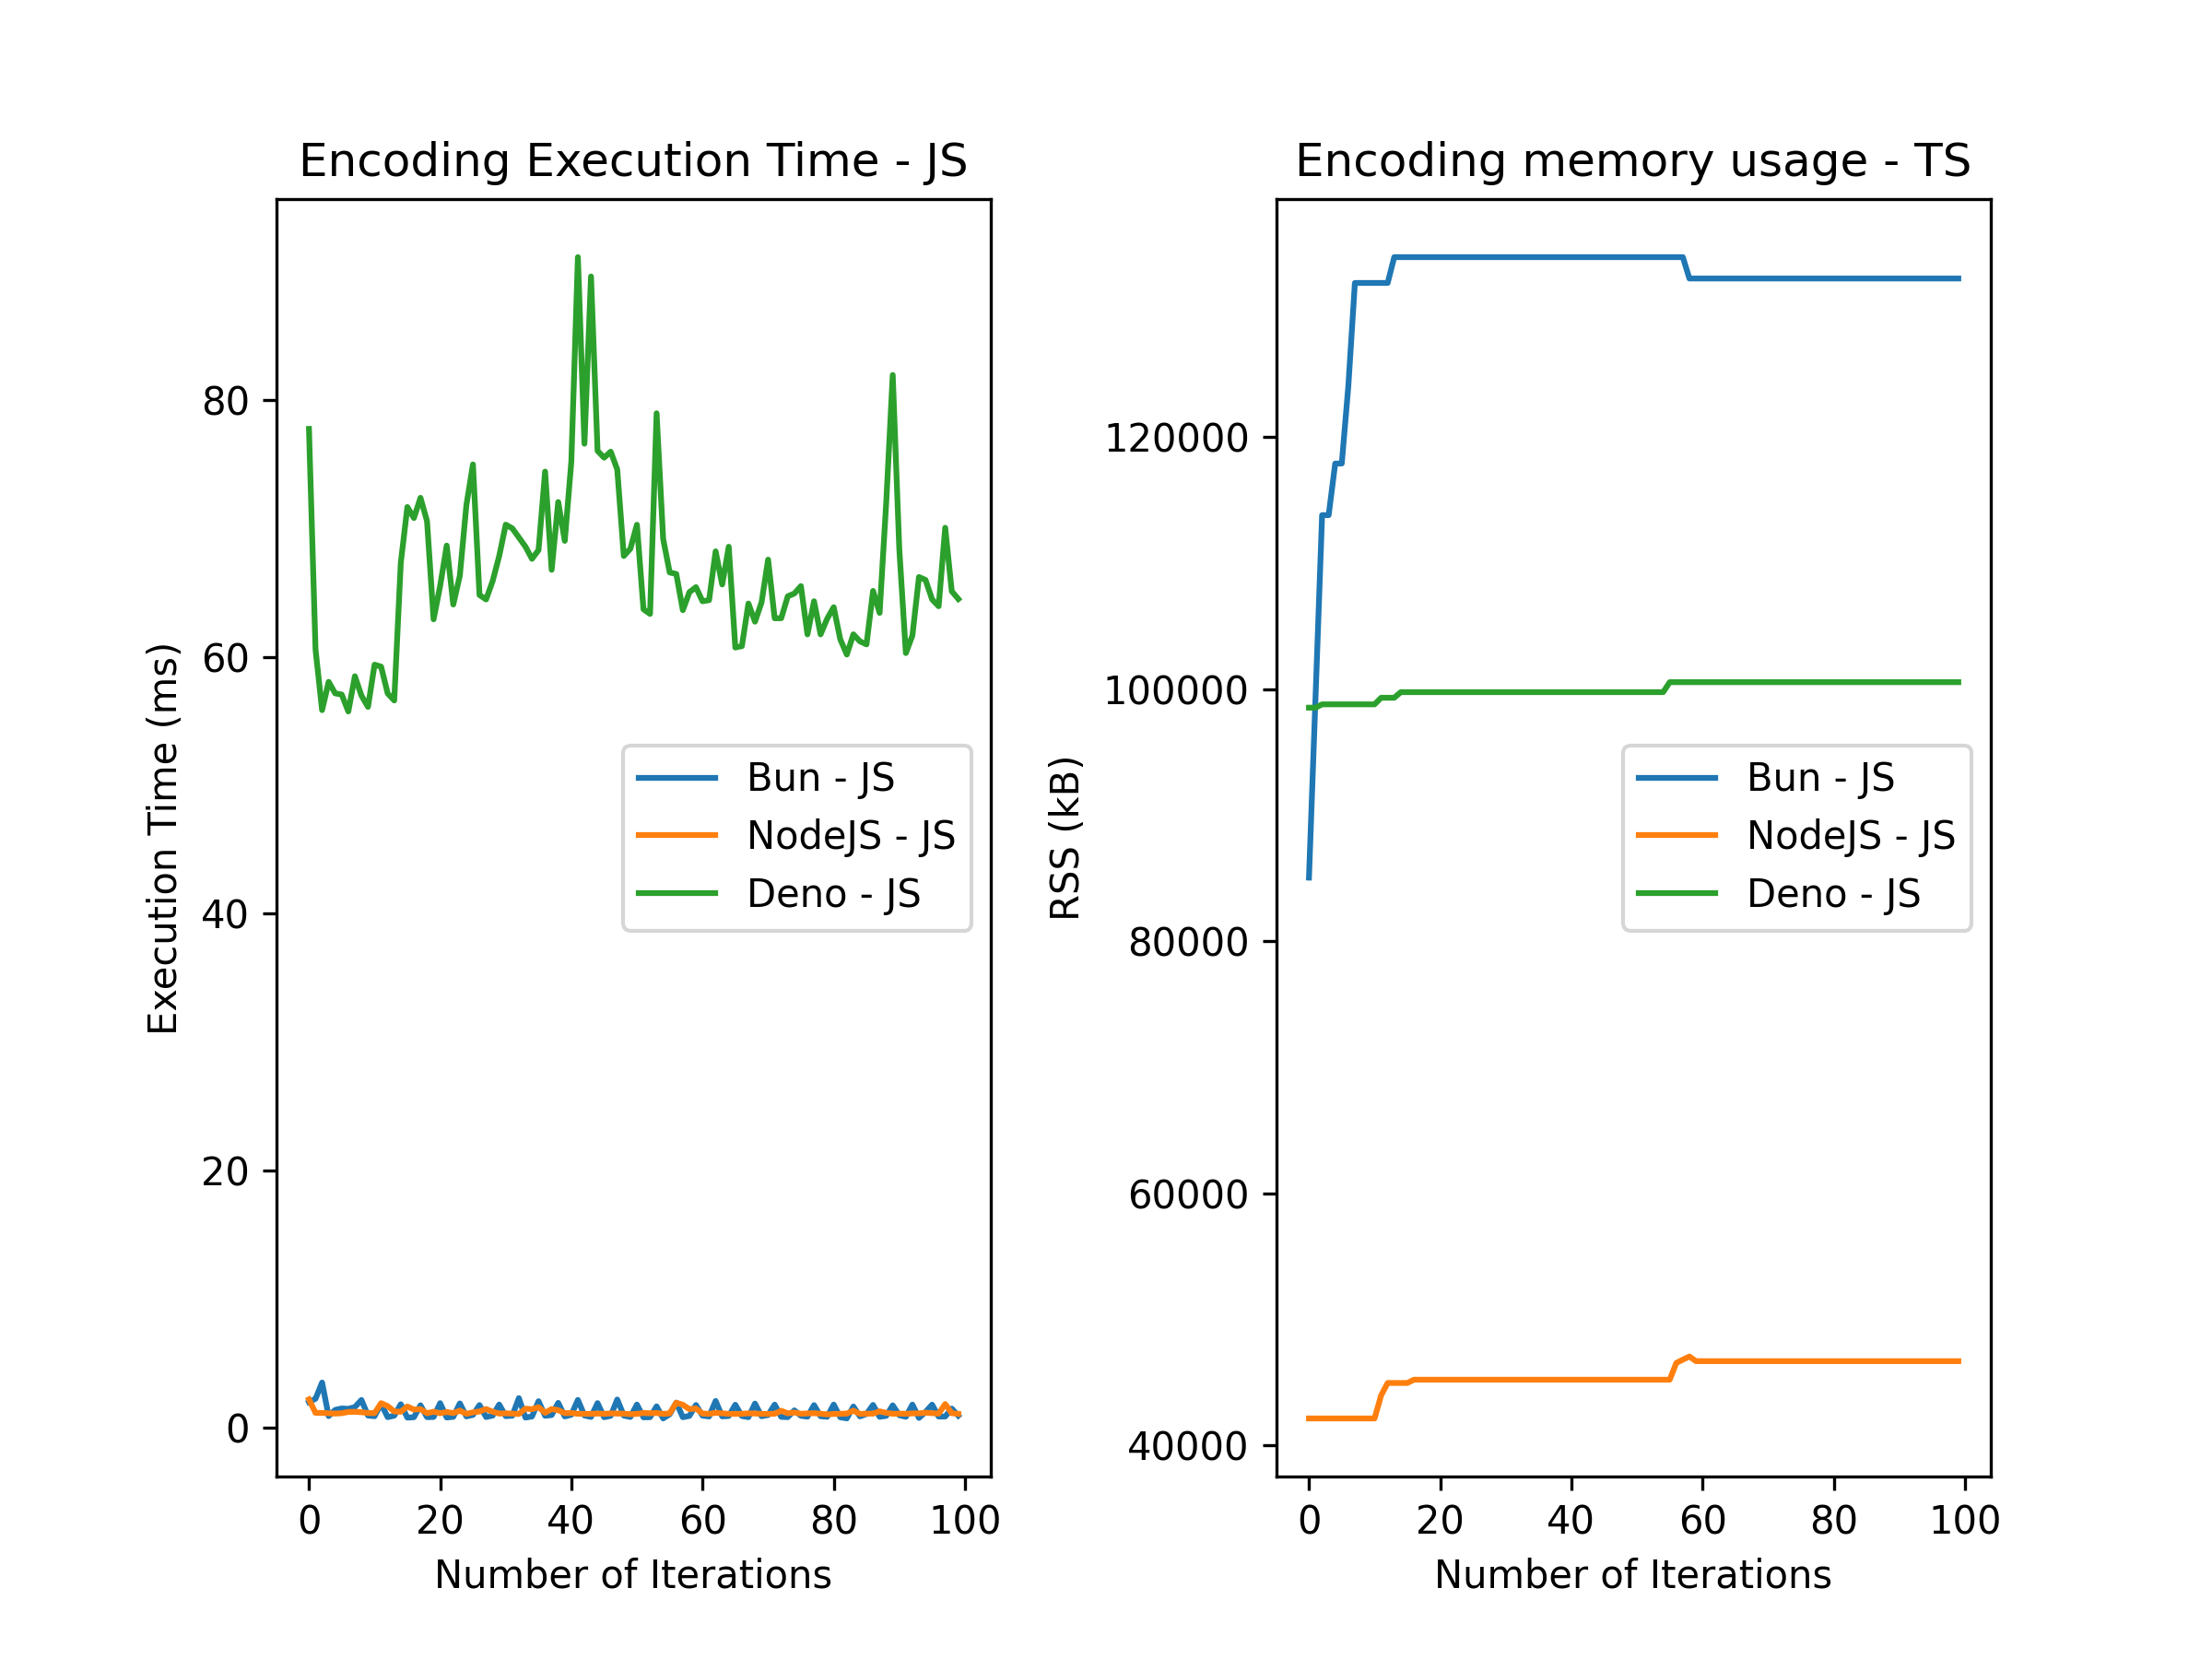
\includegraphics[width=0.68\textwidth]{Figures/coding/base64_100_encoding_js.png}
  \caption{Wyniki eksperymentów dla operacji kodowania z wykorzystaniem algorytmu \textit{Base64} dla 100 iteracji oraz 32768 znaków - po lewej czas wykonania jednorazowego testu w milisekundach, po prawej ilość zajmowanej pamięci w kilobajtach (kB)}
  \label{fig:decoding_e1_js}
\end{figure}

Na rysunku \ref{fig:encoding_e1_ts} przedstawiono wyniki eksperymentów dla operacji kodowania z wykorzystaniem algorytmu kodowania \textit{Base64} dla 100 iteracji i 32768 znaków napisanego w języku JavaScript. Na wykresie przedstawiono czas wykonania jednorazowego testu w milisekundach oraz ilość zajmowanej pamięci w kilobajtach (kB).

\begin{figure}[H]
  \centering
  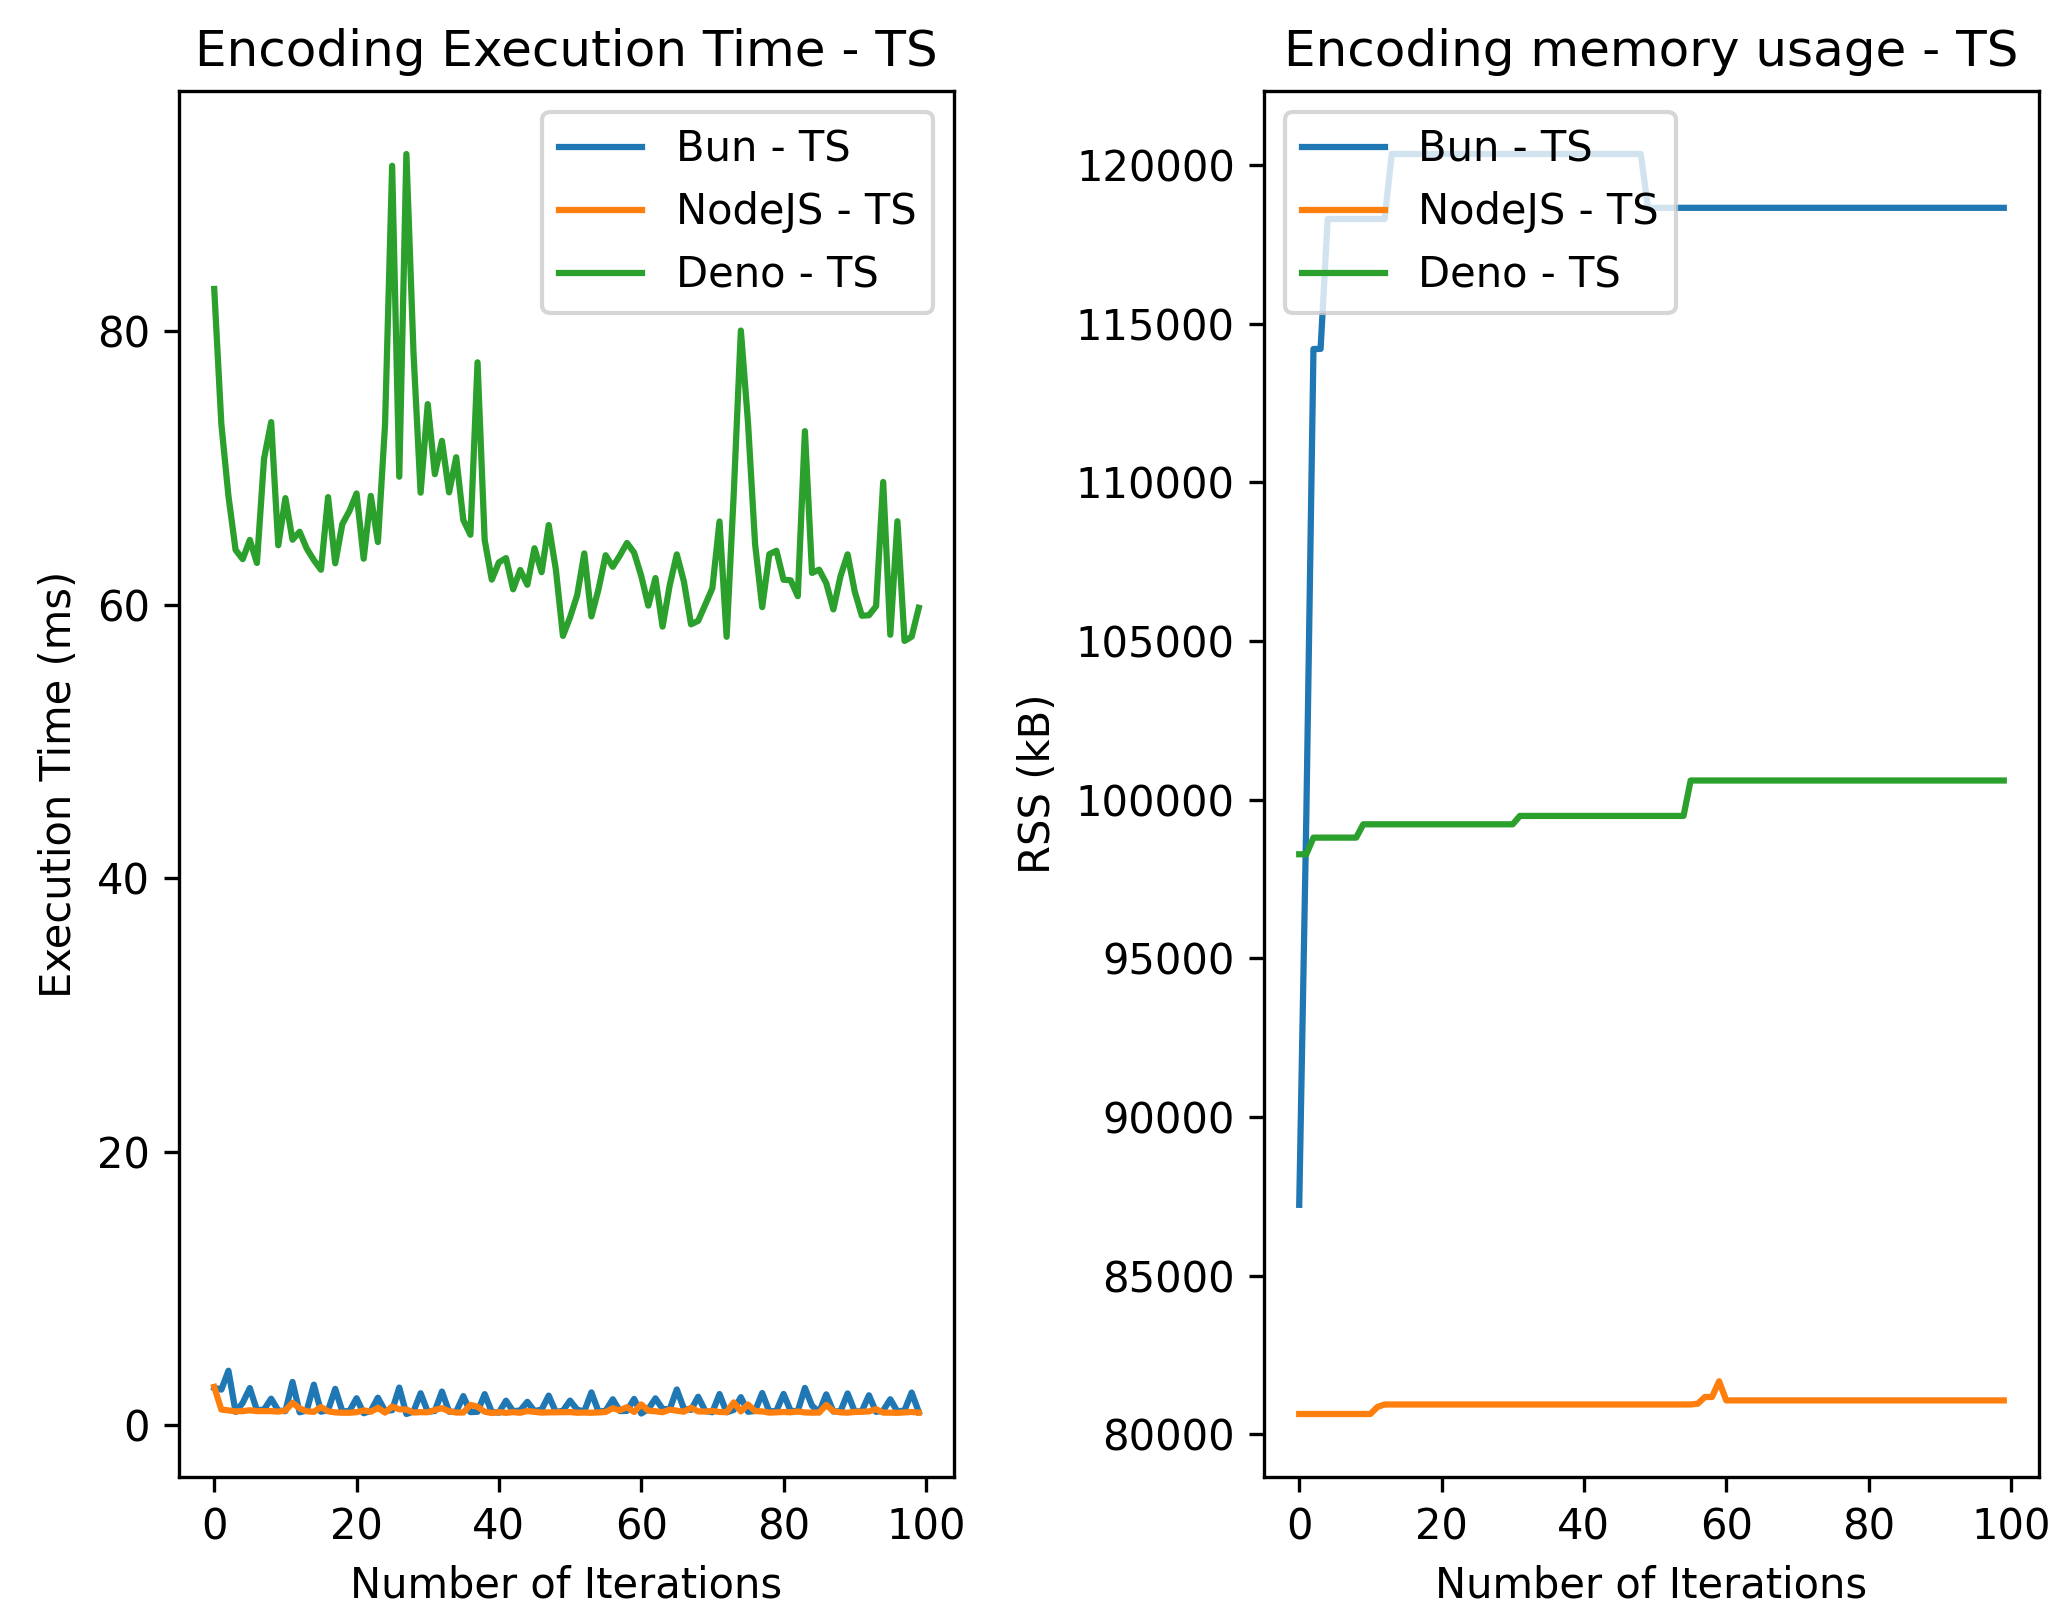
\includegraphics[width=0.68\textwidth]{Figures/coding/base64_100_encoding_ts.png}
  \caption{Wyniki eksperymentów dla operacji kodowania z wykorzystaniem algorytmu \textit{Base64} dla 100 iteracji oraz 32768 znaków - po lewej czas wykonania jednorazowego testu w milisekundach, po prawej ilość zajmowanej pamięci w kilobajtach (kB)}
  \label{fig:encoding_e1_ts}
\end{figure}

Na rysunku \ref{fig:decoding_e1_ts} przedstawiono wyniki eksperymentów dla operacji dekodowania z wykorzystaniem kodowania \textit{Base64} dla 100 iteracji i 32768 znaków napisanego w języku JavaScript. Na wykresie przedstawiono czas wykonania jednorazowego testu w milisekundach oraz ilość zajmowanej pamięci w kilobajtach (kB).

\begin{figure}[H]
  \centering
  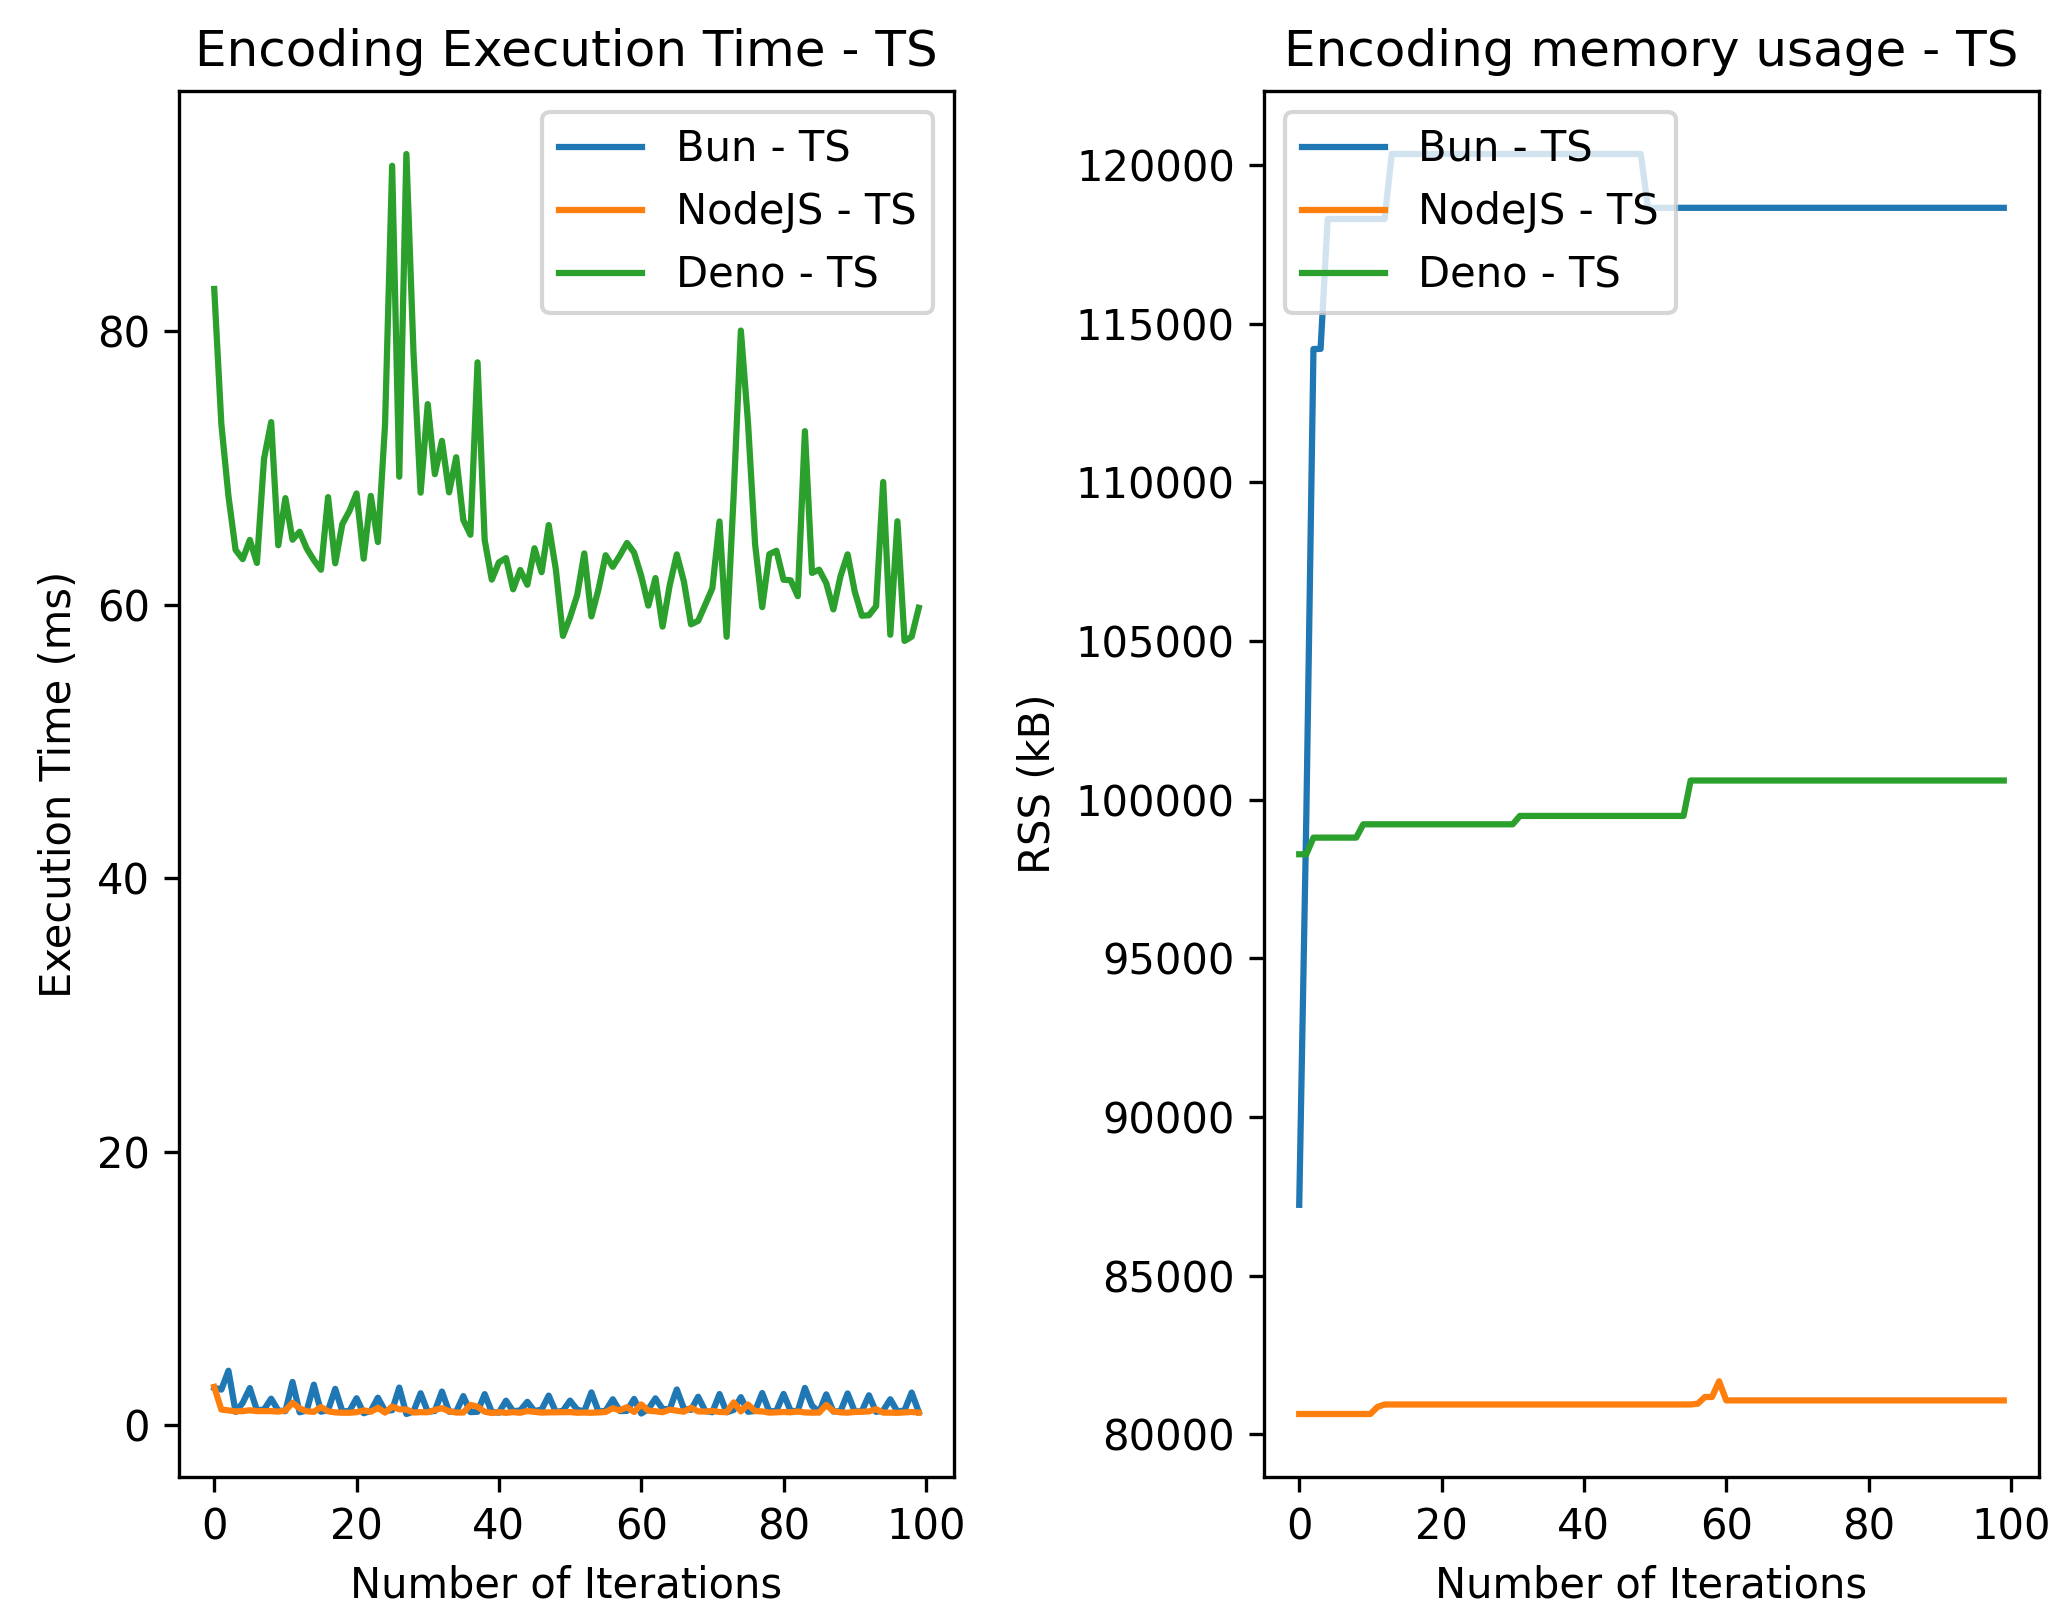
\includegraphics[width=0.68\textwidth]{Figures/coding/base64_100_encoding_ts.png}
  \caption{Wyniki eksperymentów dla operacji kodowania z wykorzystaniem algorytmu \textit{Base64} dla 100 iteracji oraz 32768 znaków - po lewej czas wykonania jednorazowego testu w milisekundach, po prawej ilość zajmowanej pamięci w kilobajtach (kB)}
  \label{fig:decoding_e1_ts}
\end{figure}

Na rysunku \ref{fig:encoding_e2_js} przedstawiono wyniki eksperymentów dla operacji kodowania z wykorzystaniem algorytmu kodowania \textit{Base64} dla 1000 iteracji i 8192 znaków napisanego w języku JavaScript. Na wykresie przedstawiono czas wykonania jednorazowego testu w milisekundach oraz ilość zajmowanej pamięci w kilobajtach (kB).

\begin{figure}[H]
  \centering
  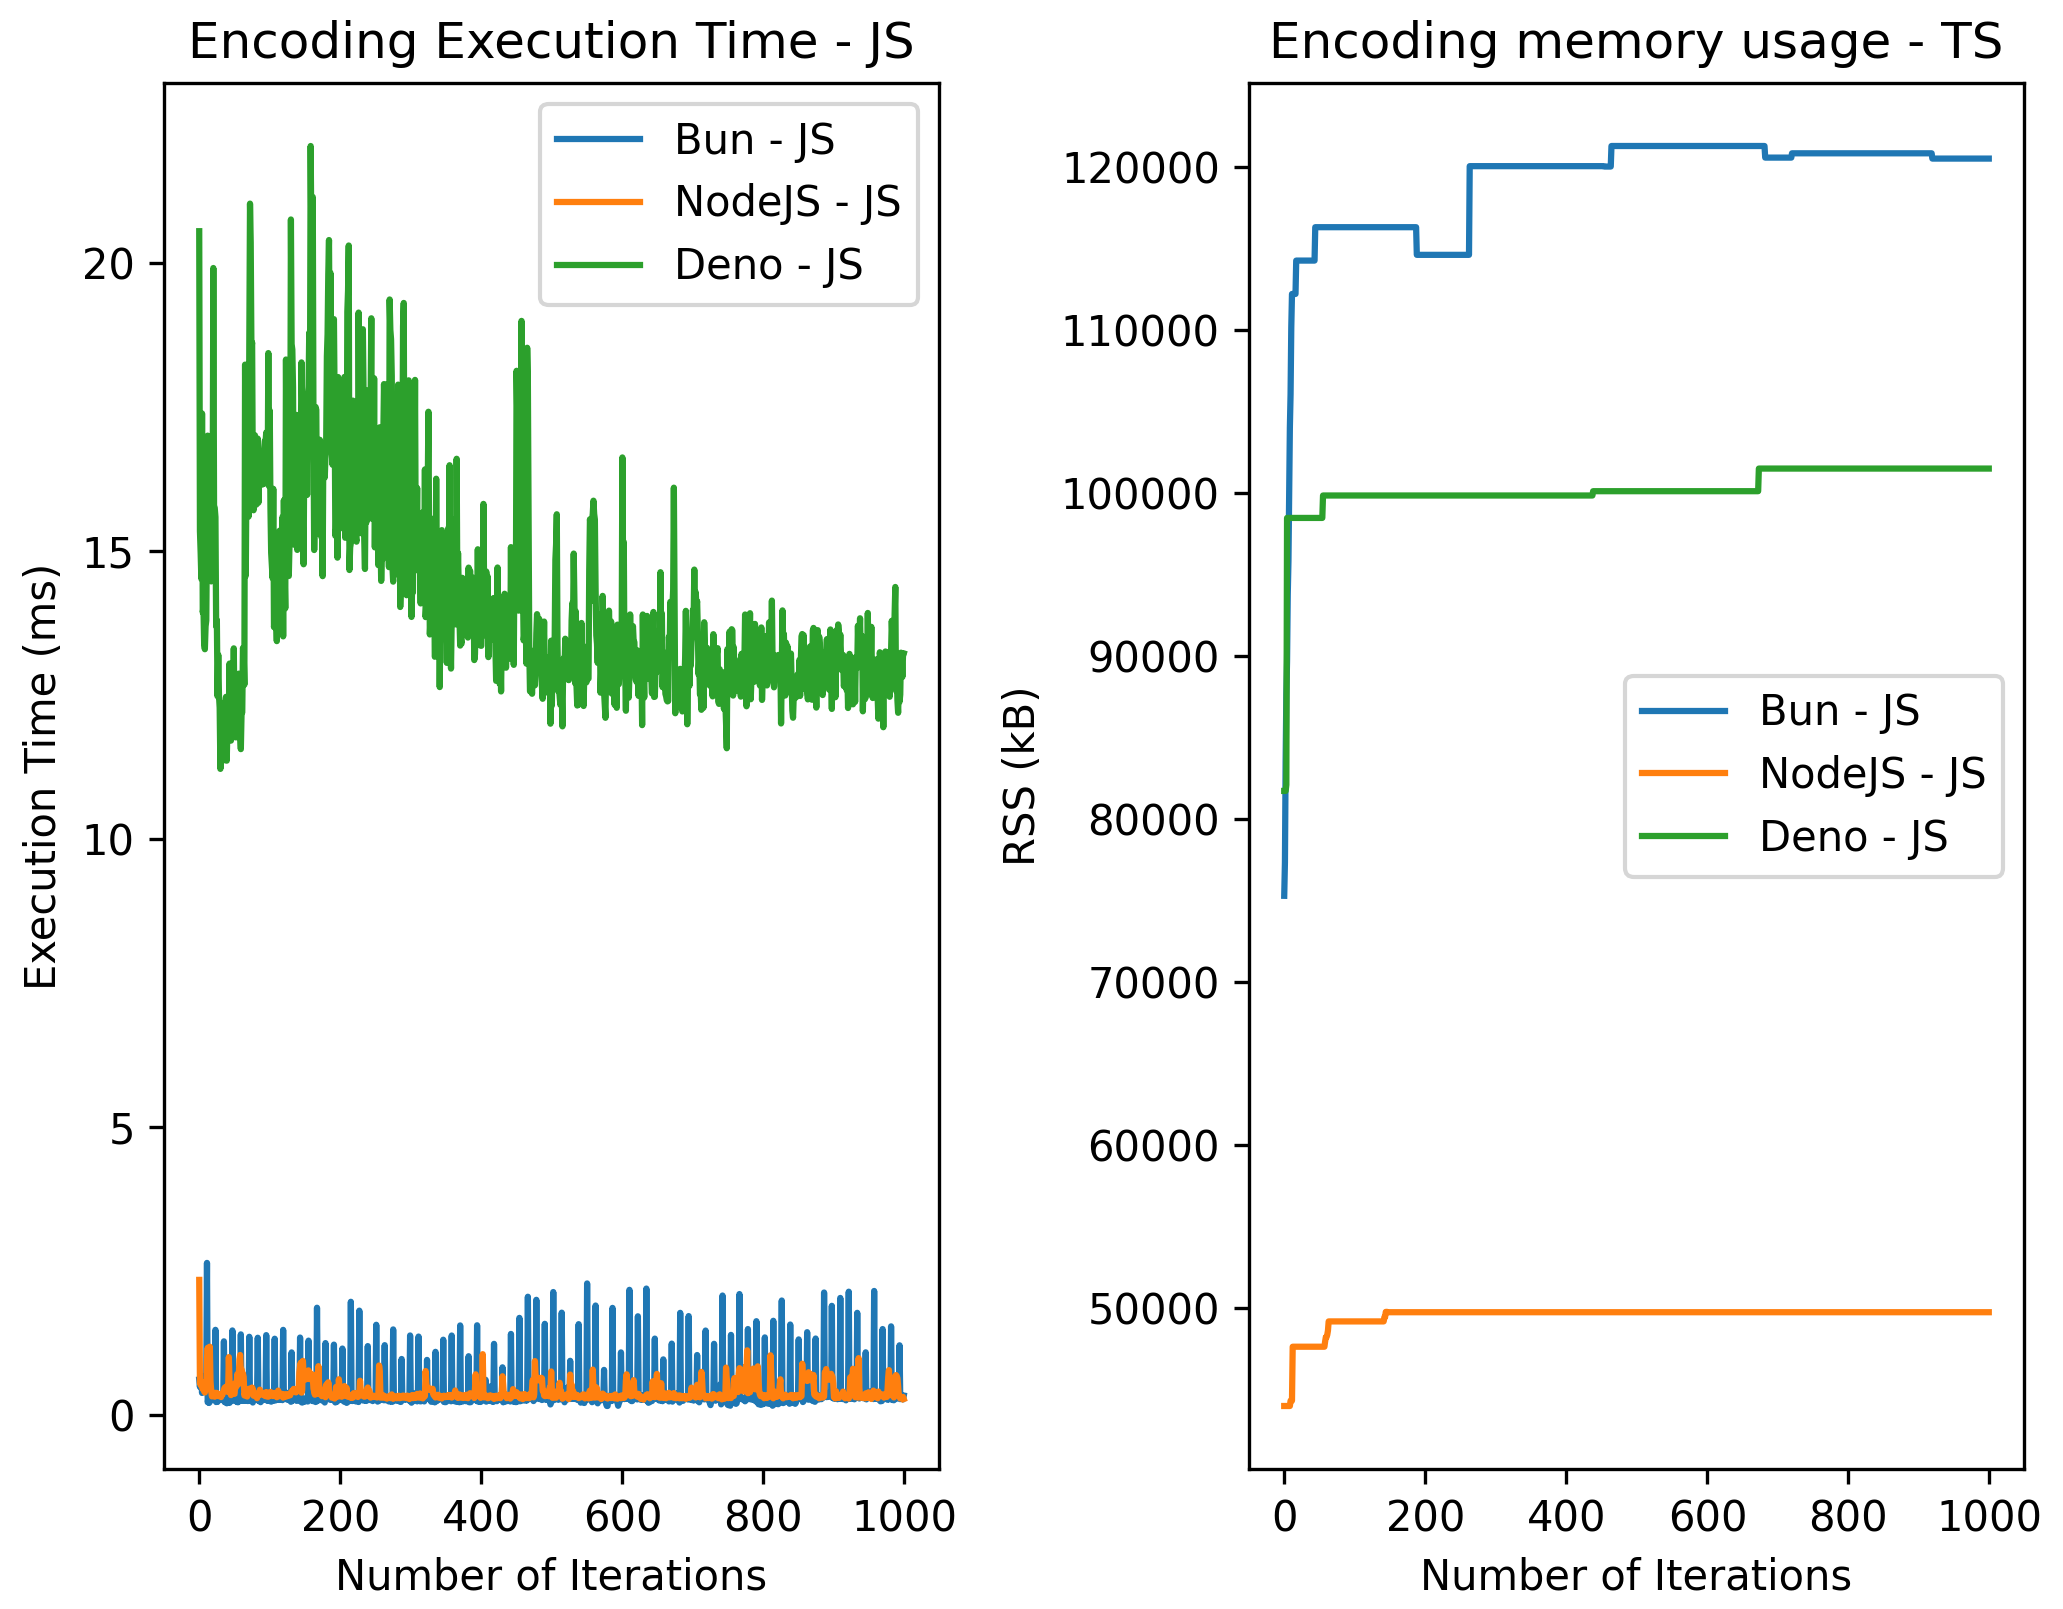
\includegraphics[width=0.68\textwidth]{Figures/coding/base64_1000_encoding_js.png}
  \caption{Wyniki eksperymentów dla operacji kodowania z wykorzystaniem algorytmu \textit{Base64} dla 1000 iteracji oraz 8192 znaków - po lewej czas wykonania jednorazowego testu w milisekundach, po prawej ilość zajmowanej pamięci w kilobajtach (kB)}
  \label{fig:encoding_e2_js}
\end{figure}

Na rysunku \ref{fig:decoding_e2_js} przedstawiono wyniki eksperymentów dla operacji dekodowania z wykorzystaniem kodowania \textit{Base64} dla 1000 iteracji i 8192 znaków napisanego w języku JavaScript. Na wykresie przedstawiono czas wykonania jednorazowego testu w milisekundach oraz ilość zajmowanej pamięci w kilobajtach (kB).

\begin{figure}[H]
  \centering
  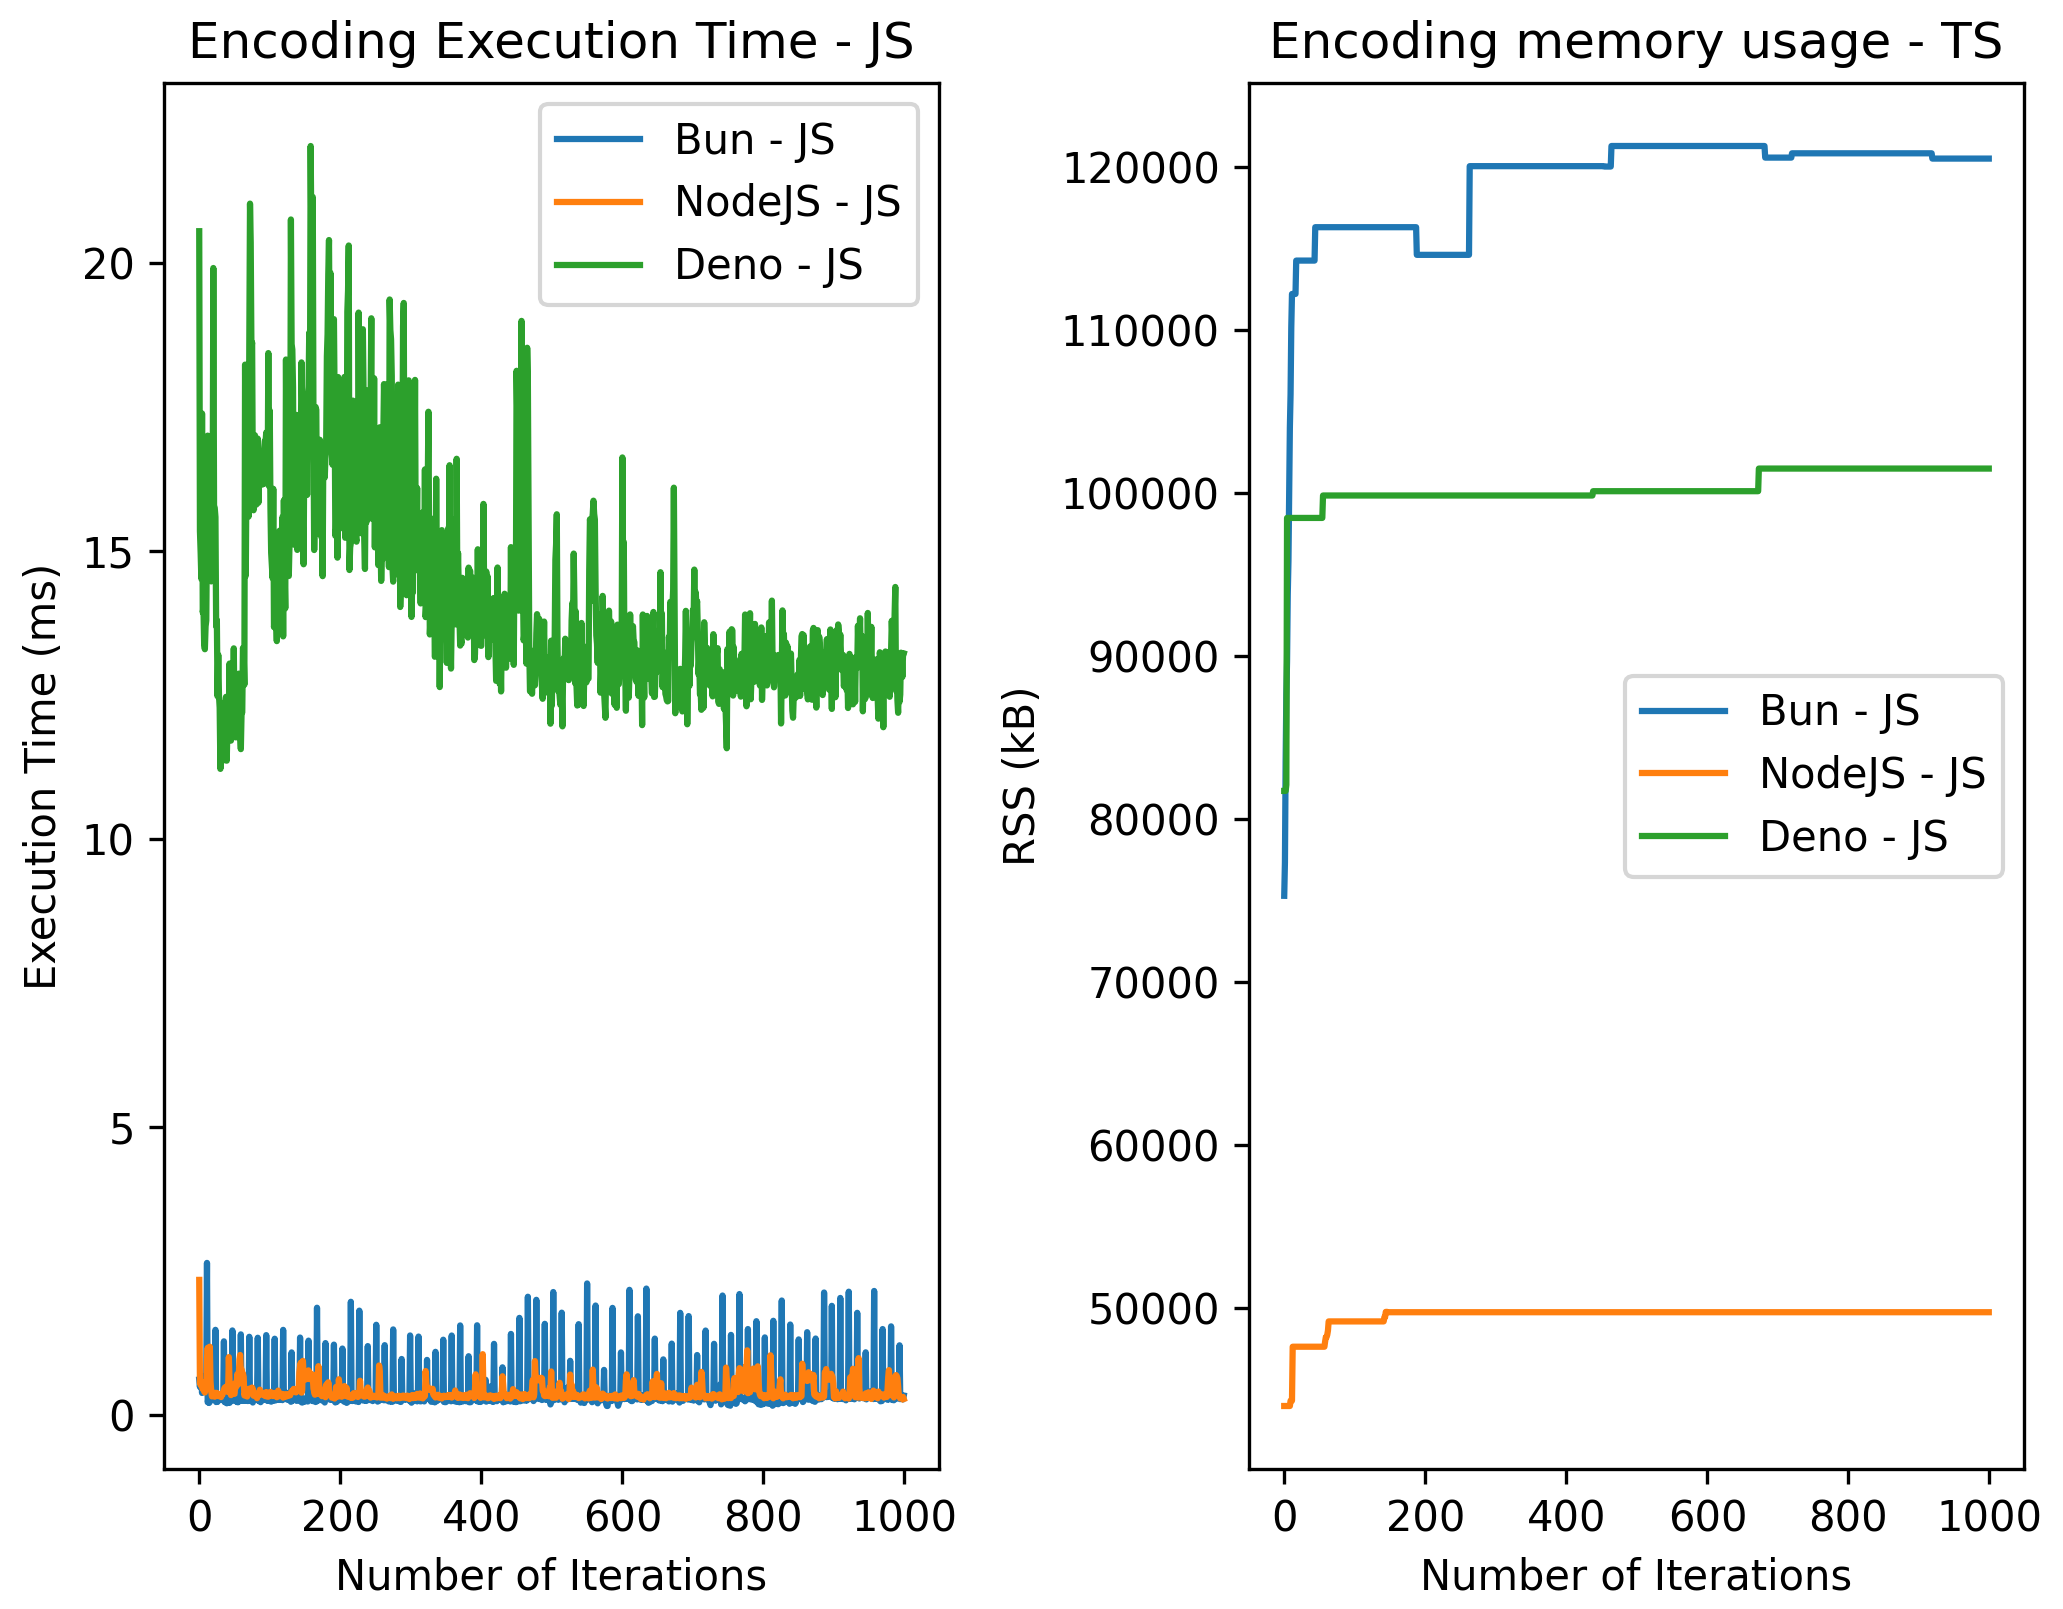
\includegraphics[width=0.68\textwidth]{Figures/coding/base64_1000_encoding_js.png}
  \caption{Wyniki eksperymentów dla operacji kodowania z wykorzystaniem algorytmu \textit{Base64} dla 1000 iteracji oraz 8192 znaków - po lewej czas wykonania jednorazowego testu w milisekundach, po prawej ilość zajmowanej pamięci w kilobajtach (kB)}
  \label{fig:decoding_e2_js}
\end{figure}

Na rysunku \ref{fig:encoding_e2_ts} przedstawiono wyniki eksperymentów dla operacji kodowania z wykorzystaniem algorytmu kodowania \textit{Base64} dla 1000 iteracji i 8192 znaków napisanego w języku JavaScript. Na wykresie przedstawiono czas wykonania jednorazowego testu w milisekundach oraz ilość zajmowanej pamięci w kilobajtach (kB).

\begin{figure}[H]
  \centering
  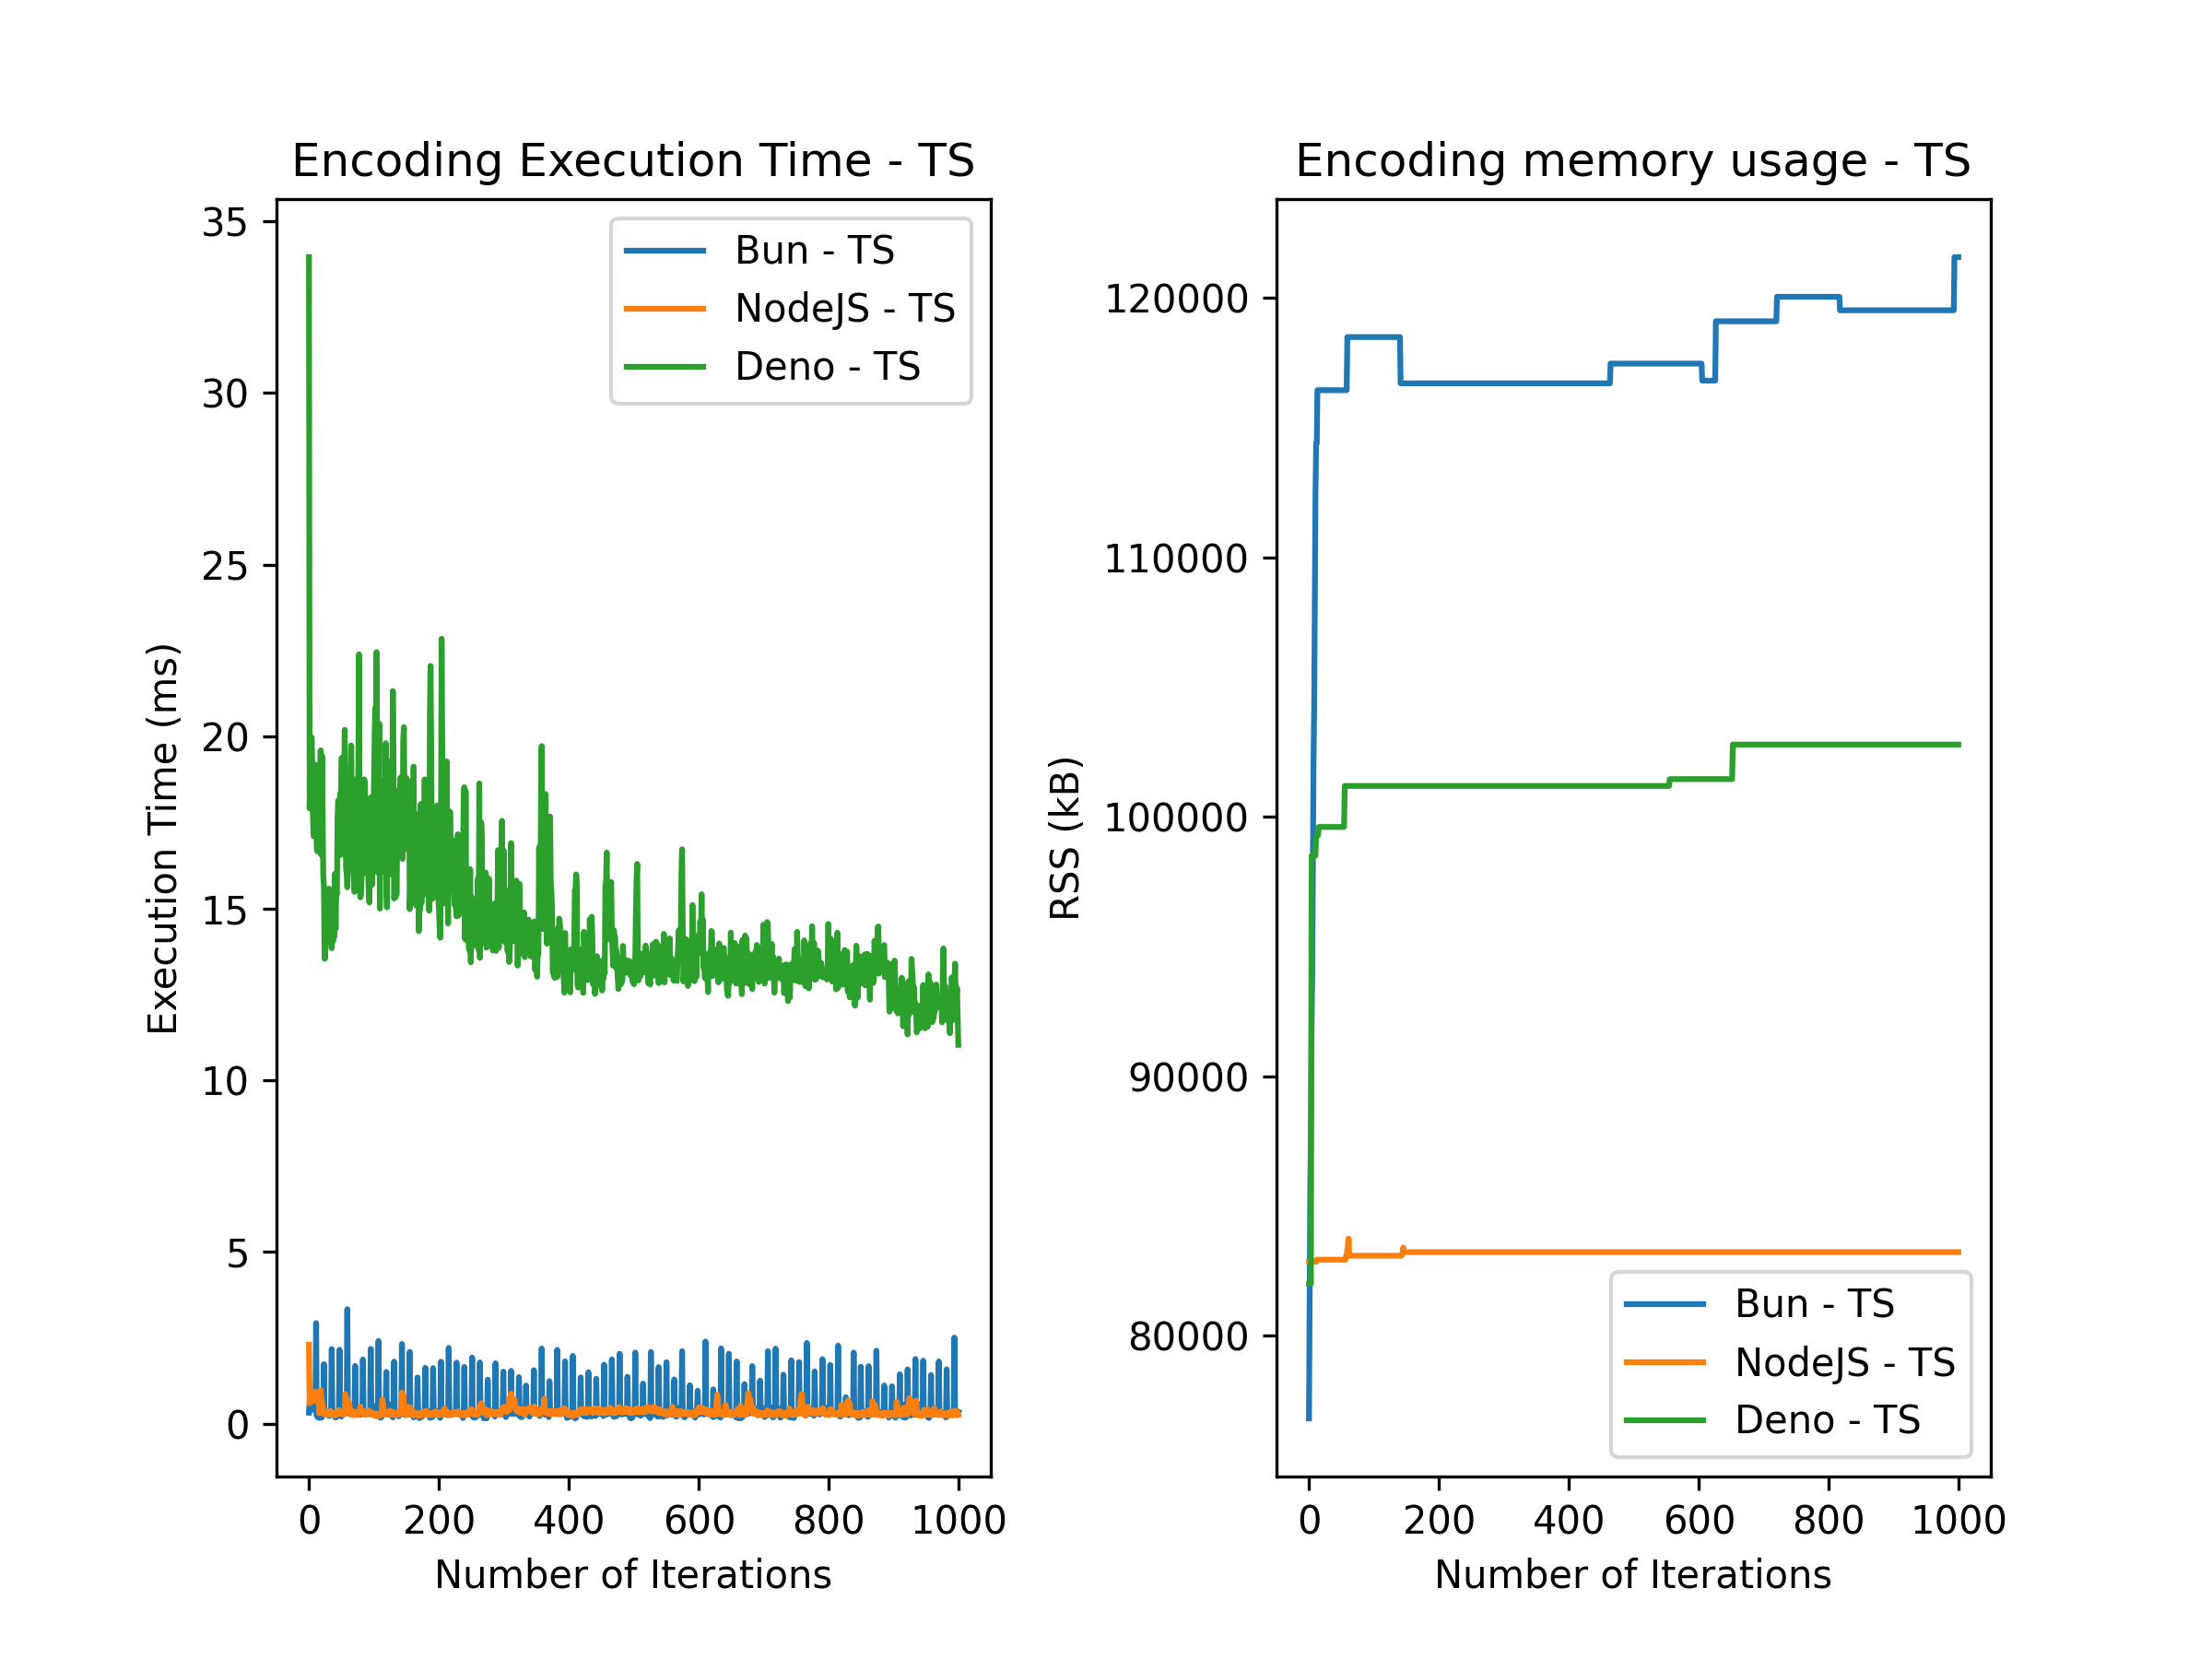
\includegraphics[width=0.68\textwidth]{Figures/coding/base64_1000_encoding_ts.png}
  \caption{Wyniki eksperymentów dla operacji kodowania z wykorzystaniem algorytmu \textit{Base64} dla 1000 iteracji oraz 8192 znaków - po lewej czas wykonania jednorazowego testu w milisekundach, po prawej ilość zajmowanej pamięci w kilobajtach (kB)}
  \label{fig:encoding_e2_ts}
\end{figure}

Na rysunku \ref{fig:decoding_e2_ts} przedstawiono wyniki eksperymentów dla operacji dekodowania z wykorzystaniem kodowania \textit{Base64} dla 100 iteracji i 8192 znaków napisanego w języku JavaScript. Na wykresie przedstawiono czas wykonania jednorazowego testu w milisekundach oraz ilość zajmowanej pamięci w kilobajtach (kB).

\begin{figure}[H]
  \centering
  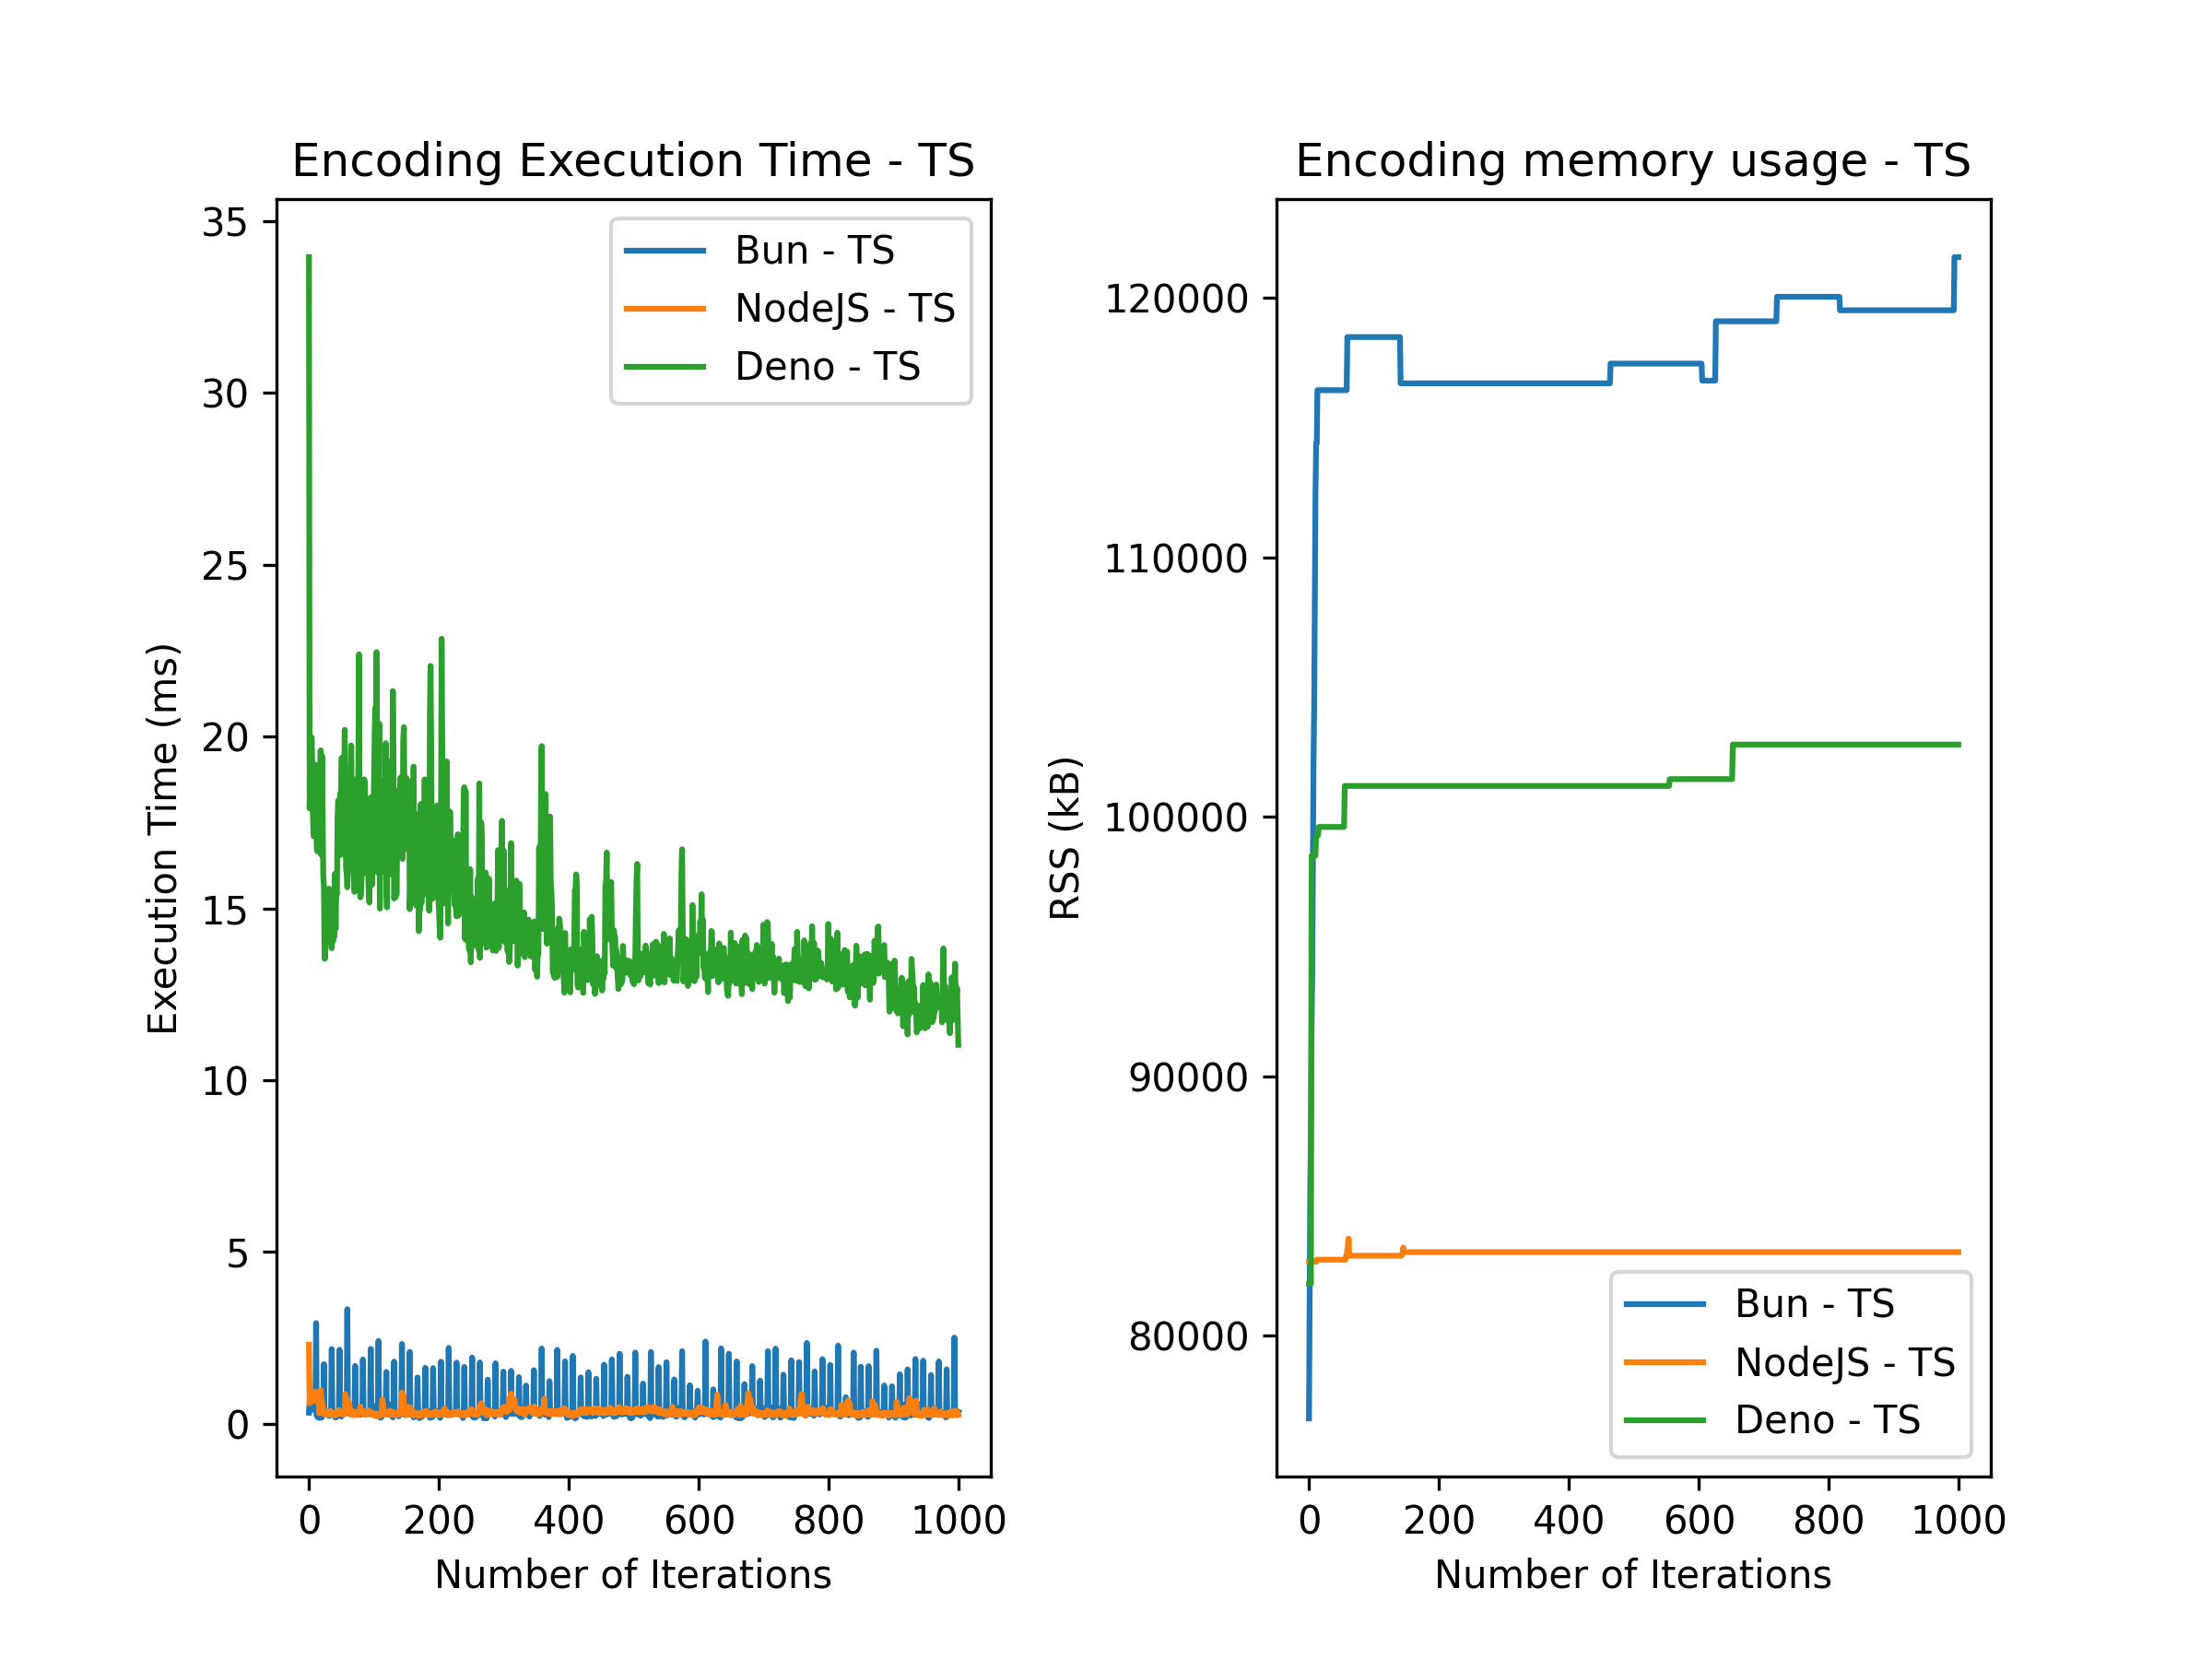
\includegraphics[width=0.68\textwidth]{Figures/coding/base64_1000_encoding_ts.png}
  \caption{Wyniki eksperymentów dla operacji kodowania z wykorzystaniem algorytmu \textit{Base64} dla 1000 iteracji oraz 8192 znaków - po lewej czas wykonania jednorazowego testu w milisekundach, po prawej ilość zajmowanej pamięci w kilobajtach (kB)}
  \label{fig:decoding_e2_ts}
\end{figure}

\subsection{Testy wydajnościowe operacji zapisu i odczytu plików}
W celu zbadania wydajności operacji zapisu oraz odczytu plików, przeprowadzono eksperymenty, które polegały na zapisie oraz odczycie plików o różnych rozmiarach. W przeprowadzonych testach wykorzystano pliki tekstowe, natomiast zawartość plików została wygenerowana za pomocą modułu \textit{faker.js}. W tym celu generowano paragrafy tekstu. W tabeli \ref{tab:file_experiments} przedstawiono liczbę przeprowadzonych eksperymentów oraz rozmiar pliku.

\begin{table}[H]
  \centering
  \caption{Parametry eksperymentów zapisu i odczytu plików}
  \begin{tabular}{|c|c|c|}
    \hline
    \textbf{Ilość eksperymentów} & \textbf{Rozmiar pliku} & \textbf{Ilość plików} \\ \hline
    50 & 512kB & 50 \\ \hline
    50 & 1MB & 50 \\ \hline
  \end{tabular}
  \label{tab:file_experiments}
\end{table}

\subsubsection{Wyniki}
Na rysunku \ref{fig:file_e1_reading_js} przedstawiono wyniki eksperymentów dla operacji zapisu dla 50 iteracji oraz 50 plików o rozmiarze 512kB napisanego w języku JavaScript. Na wykresie przedstawiono czas wykonania jednorazowego testu w milisekundach oraz ilość zajmowanej pamięci w kilobajtach (kB).

\begin{figure}[H]
  \centering
  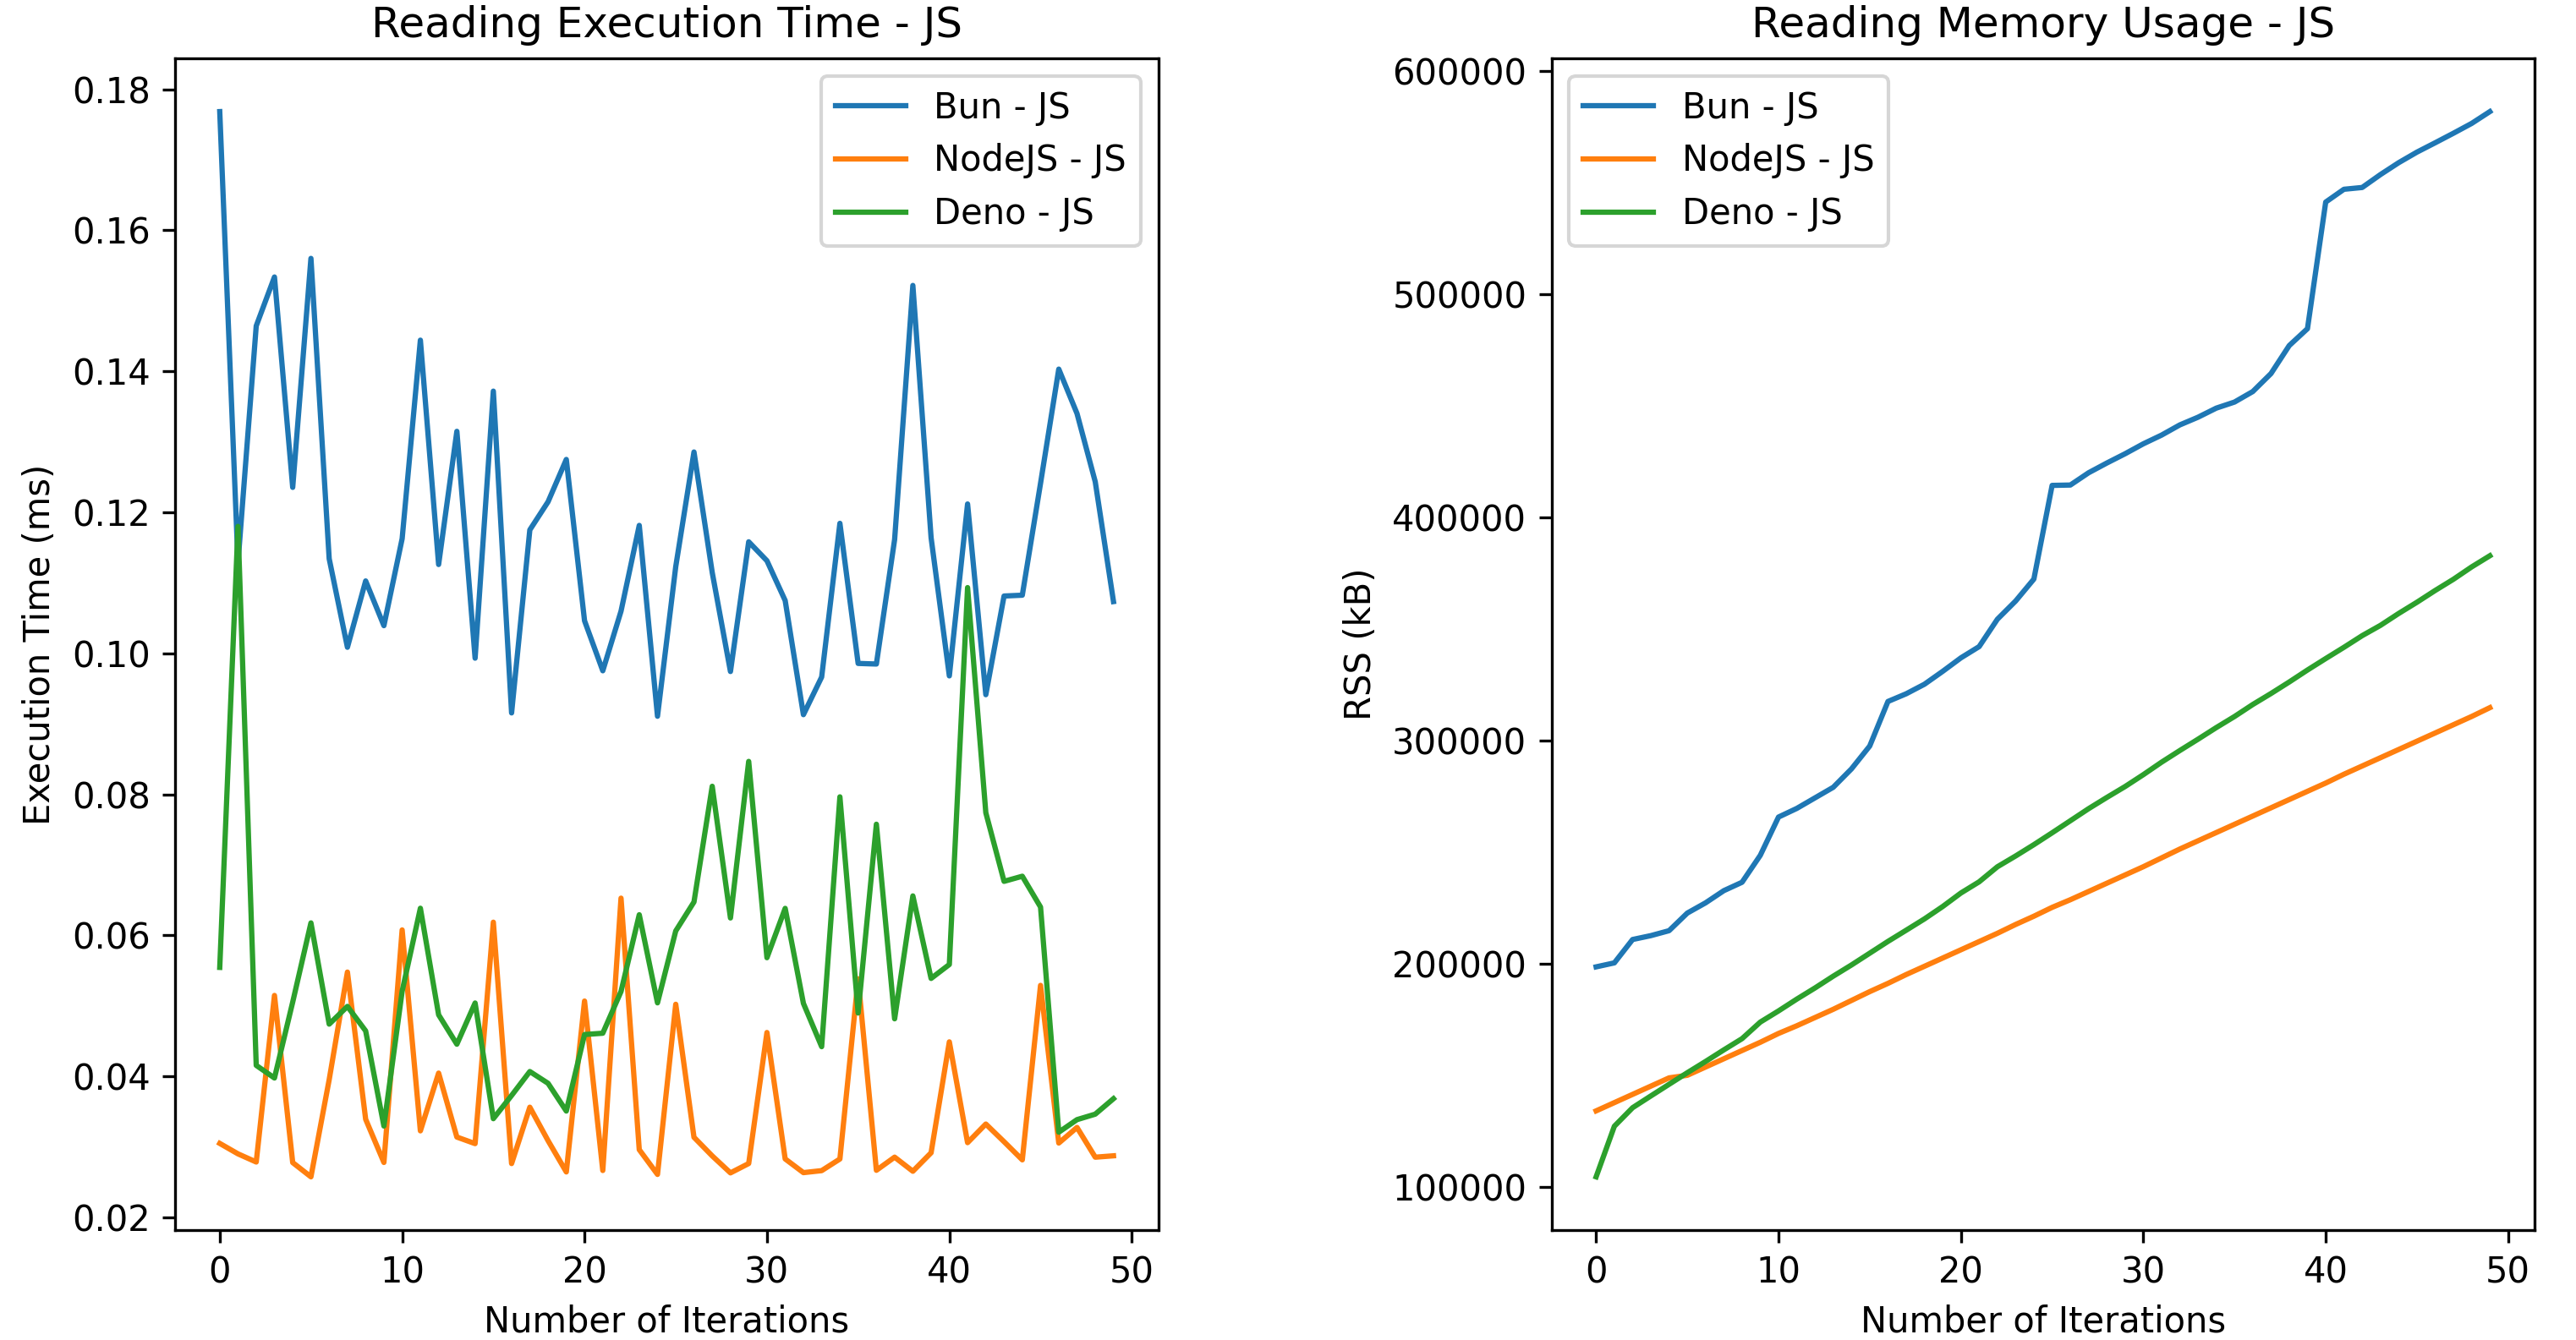
\includegraphics[width=0.68\textwidth]{Figures/files/files_reading_50_500_50_js.png}
  \caption{Wynik eksperymentów zapisu pliku dla 50 iteracji oraz 50 plików o rozmiarze 512kB - po lewej czas wykonania jednorazowego testu w milisekundach, po prawej ilość zajmowanej pamięci w kilobajtach (kB)}
  \label{fig:file_e1_reading_js}
\end{figure}

Na rysunku \ref{fig:file_e1_writing_js} przedstawiono wyniki eksperymentów dla operacji odczytu dla 50 iteracji oraz 50 plików o rozmiarze 512kB napisanego w języku JavaScript. Na wykresie przedstawiono czas wykonania jednorazowego testu w milisekundach oraz ilość zajmowanej pamięci w kilobajtach (kB).

\begin{figure}[H]
  \centering
  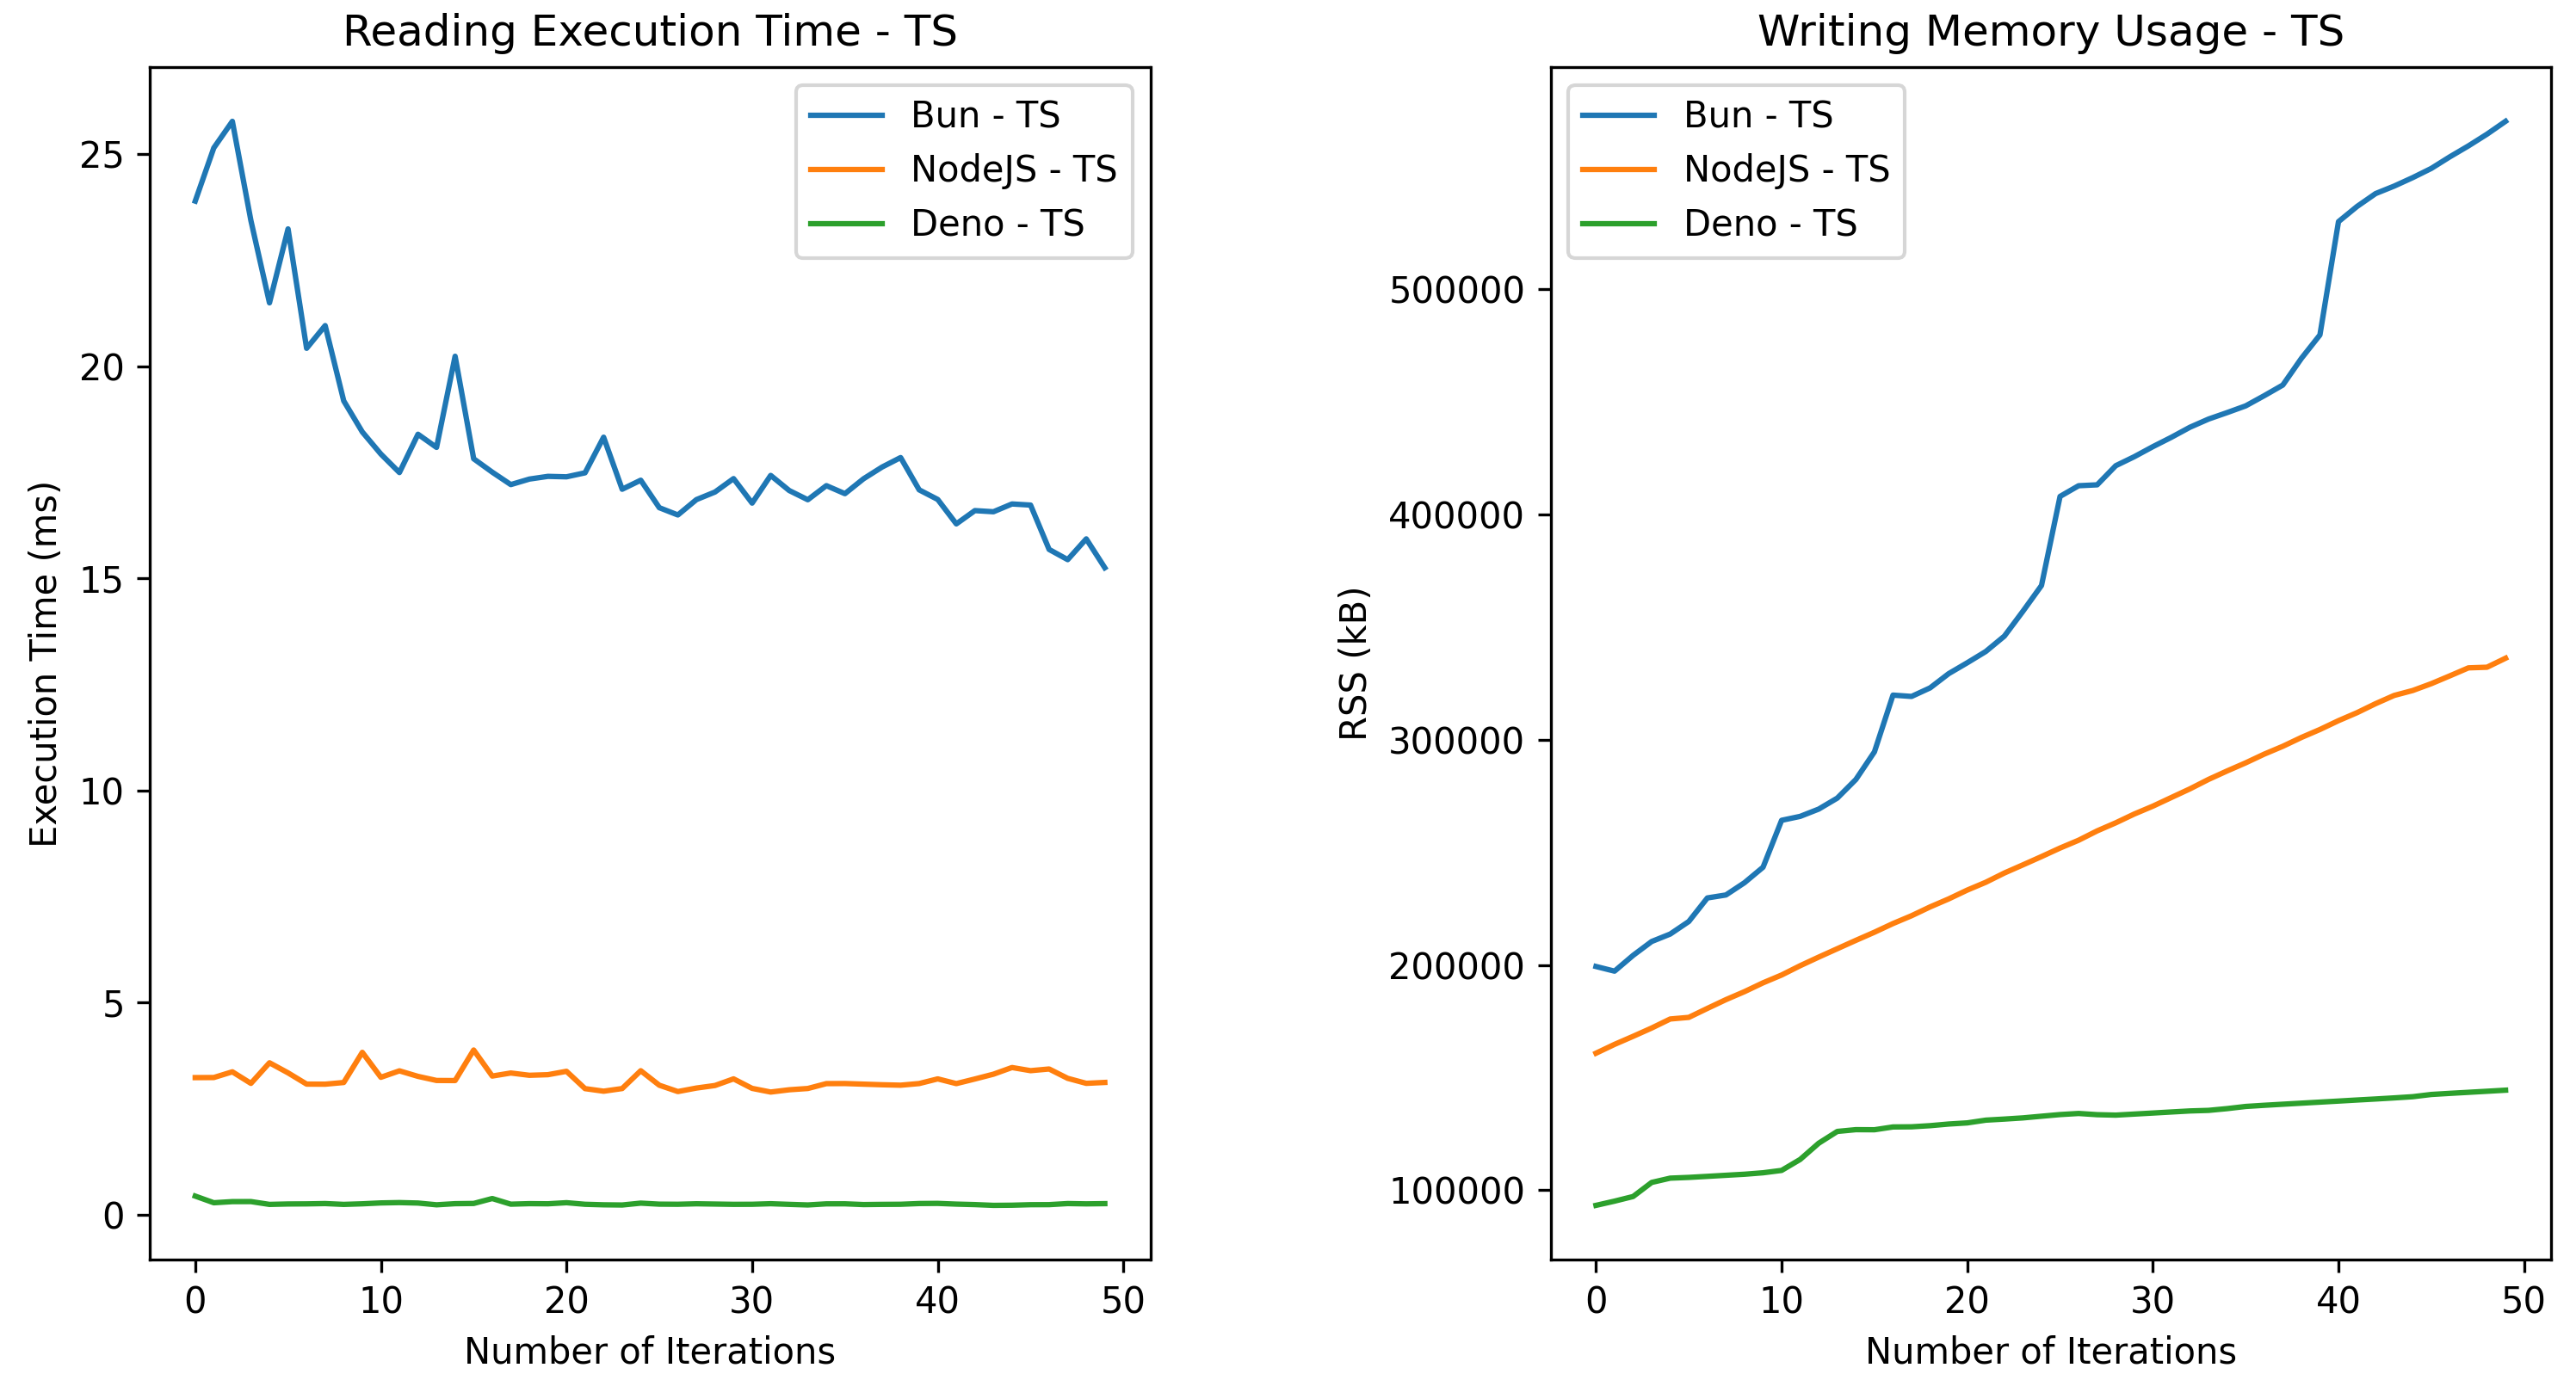
\includegraphics[width=0.68\textwidth]{Figures/files/files_writing_50_500_50_ts.png}
  \caption{Wynik eksperymentów zapisu pliku dla 50 iteracji oraz 50 plików o rozmiarze 512kB - po lewej czas wykonania jednorazowego testu w milisekundach, po prawej ilość zajmowanej pamięci w kilobajtach (kB)}
  \label{fig:file_e1_writing_js}
\end{figure}

Na rysunku \ref{fig:file_e1_reading_ts} przedstawiono wyniki eksperymentów dla operacji zapisu dla 50 iteracji oraz 50 plików o rozmiarze 512kB napisanego w języku TypeScript. Na wykresie przedstawiono czas wykonania jednorazowego testu w milisekundach oraz ilość zajmowanej pamięci w kilobajtach (kB).

\begin{figure}[H]
  \centering
  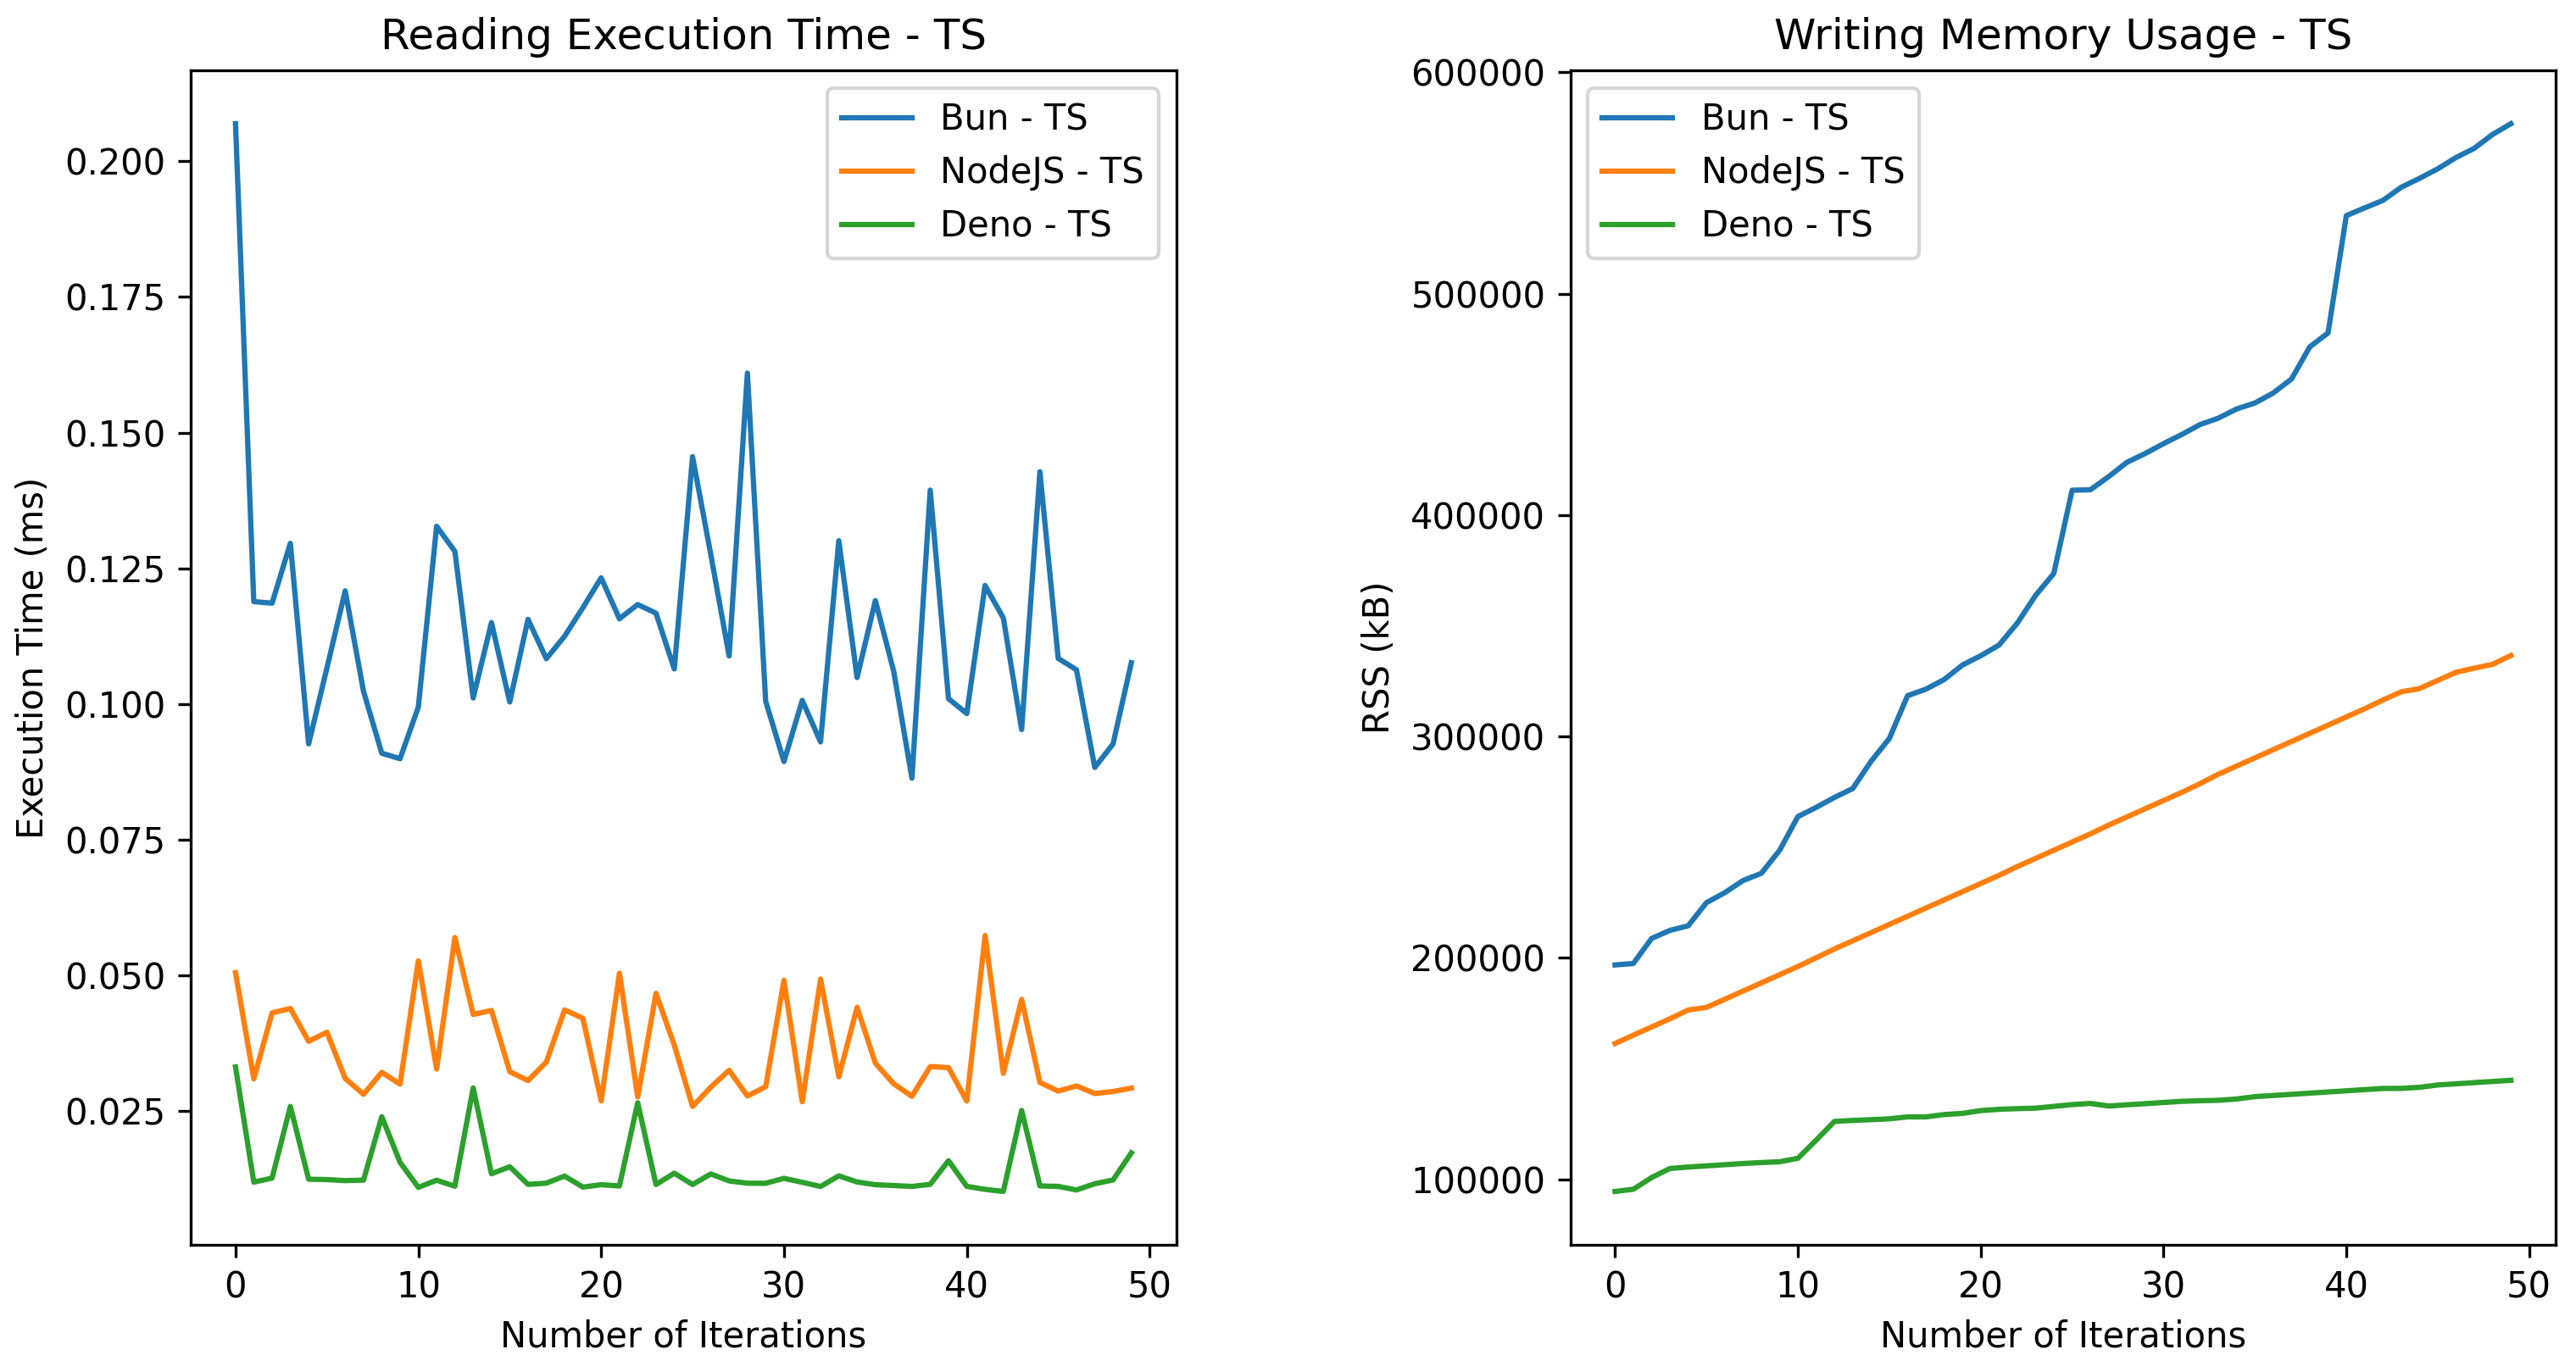
\includegraphics[width=0.68\textwidth]{Figures/files/files_reading_50_500_50_ts.png}
  \caption{Wynik eksperymentów zapisu pliku dla 50 iteracji oraz 50 plików o rozmiarze 512kB - po lewej czas wykonania jednorazowego testu w milisekundach, po prawej ilość zajmowanej pamięci w kilobajtach (kB)}
  \label{fig:file_e1_reading_ts}
\end{figure}

Na rysunku \ref{fig:file_e1_writing_ts} przedstawiono wyniki eksperymentów dla operacji odczytu dla 50 iteracji oraz 50 plików o rozmiarze 512kB napisanego w języku TypeScript. Na wykresie przedstawiono czas wykonania jednorazowego testu w milisekundach oraz ilość zajmowanej pamięci w kilobajtach (kB).

\begin{figure}[H]
  \centering
  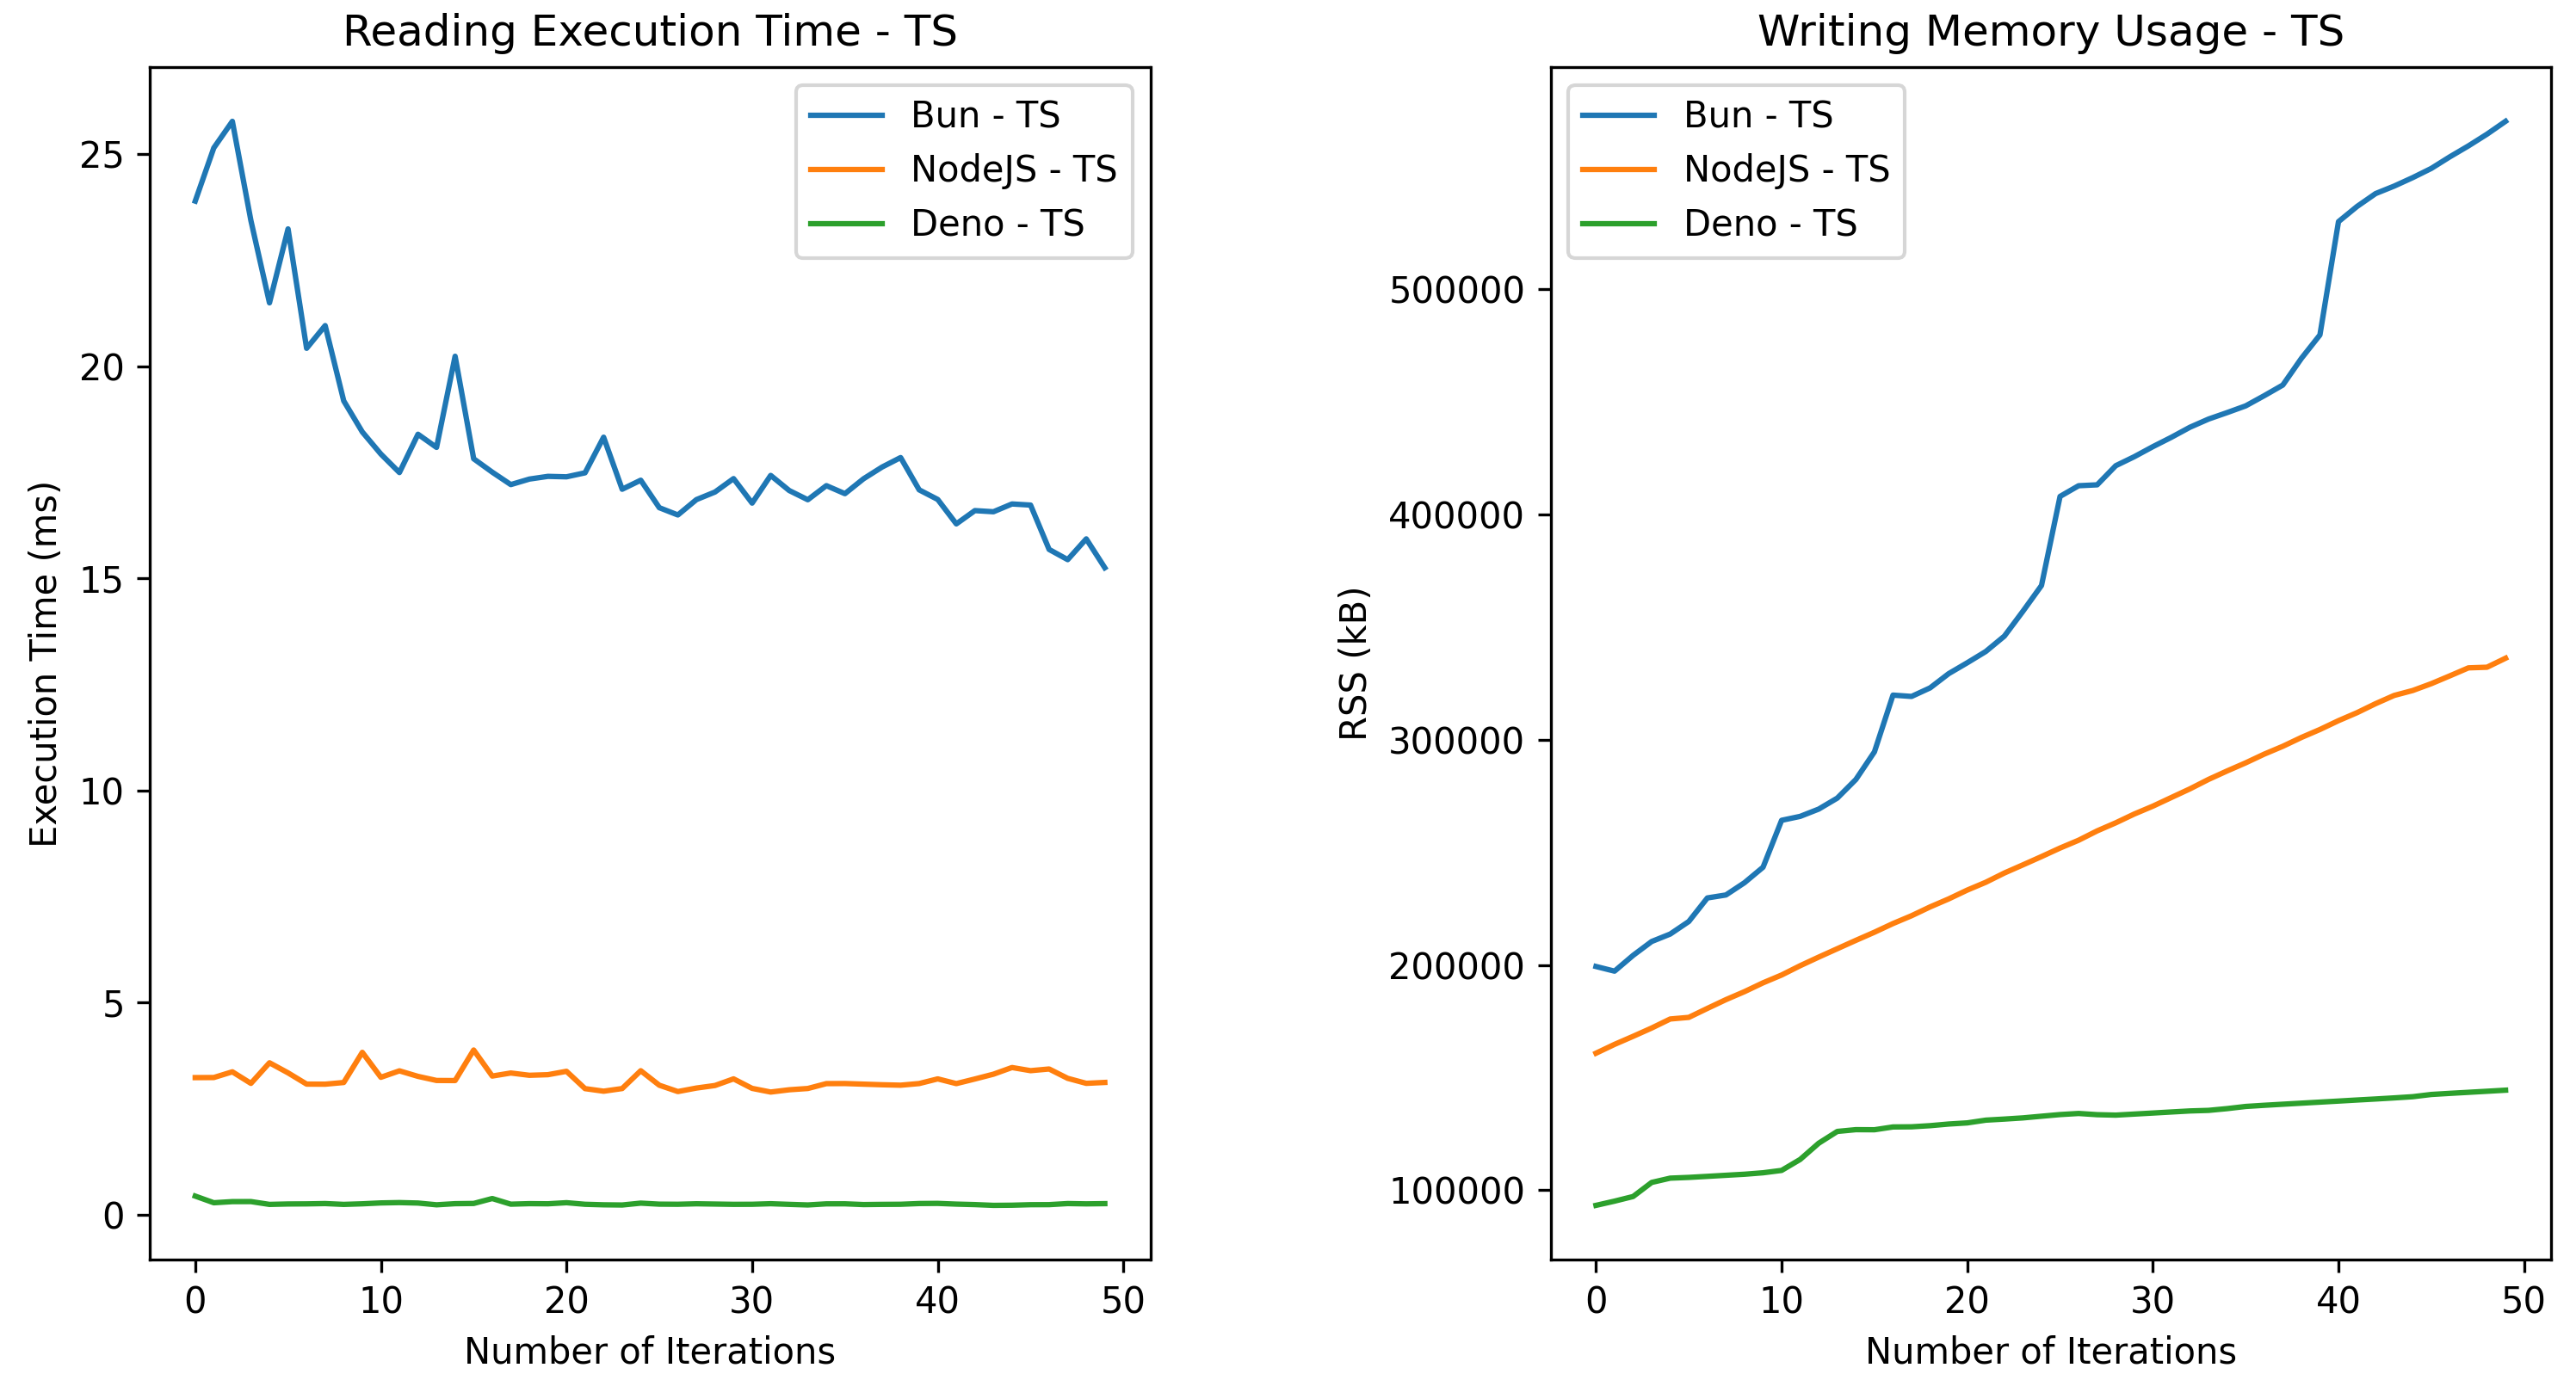
\includegraphics[width=0.68\textwidth]{Figures/files/files_writing_50_500_50_ts.png}
  \caption{Wynik eksperymentów zapisu pliku dla 50 iteracji oraz 50 plików o rozmiarze 512kB - po lewej czas wykonania jednorazowego testu w milisekundach, po prawej ilość zajmowanej pamięci w kilobajtach (kB)}
  \label{fig:file_e1_writing_ts}
\end{figure}

Na rysunku \ref{fig:file_e2_reading_js} przedstawiono wyniki eksperymentów dla operacji zapisu dla 50 iteracji oraz 50 plików o rozmiarze 1MB napisanego w języku JavaScript. Na wykresie przedstawiono czas wykonania jednorazowego testu w milisekundach oraz ilość zajmowanej pamięci w kilobajtach (kB).

\begin{figure}[H]
  \centering
  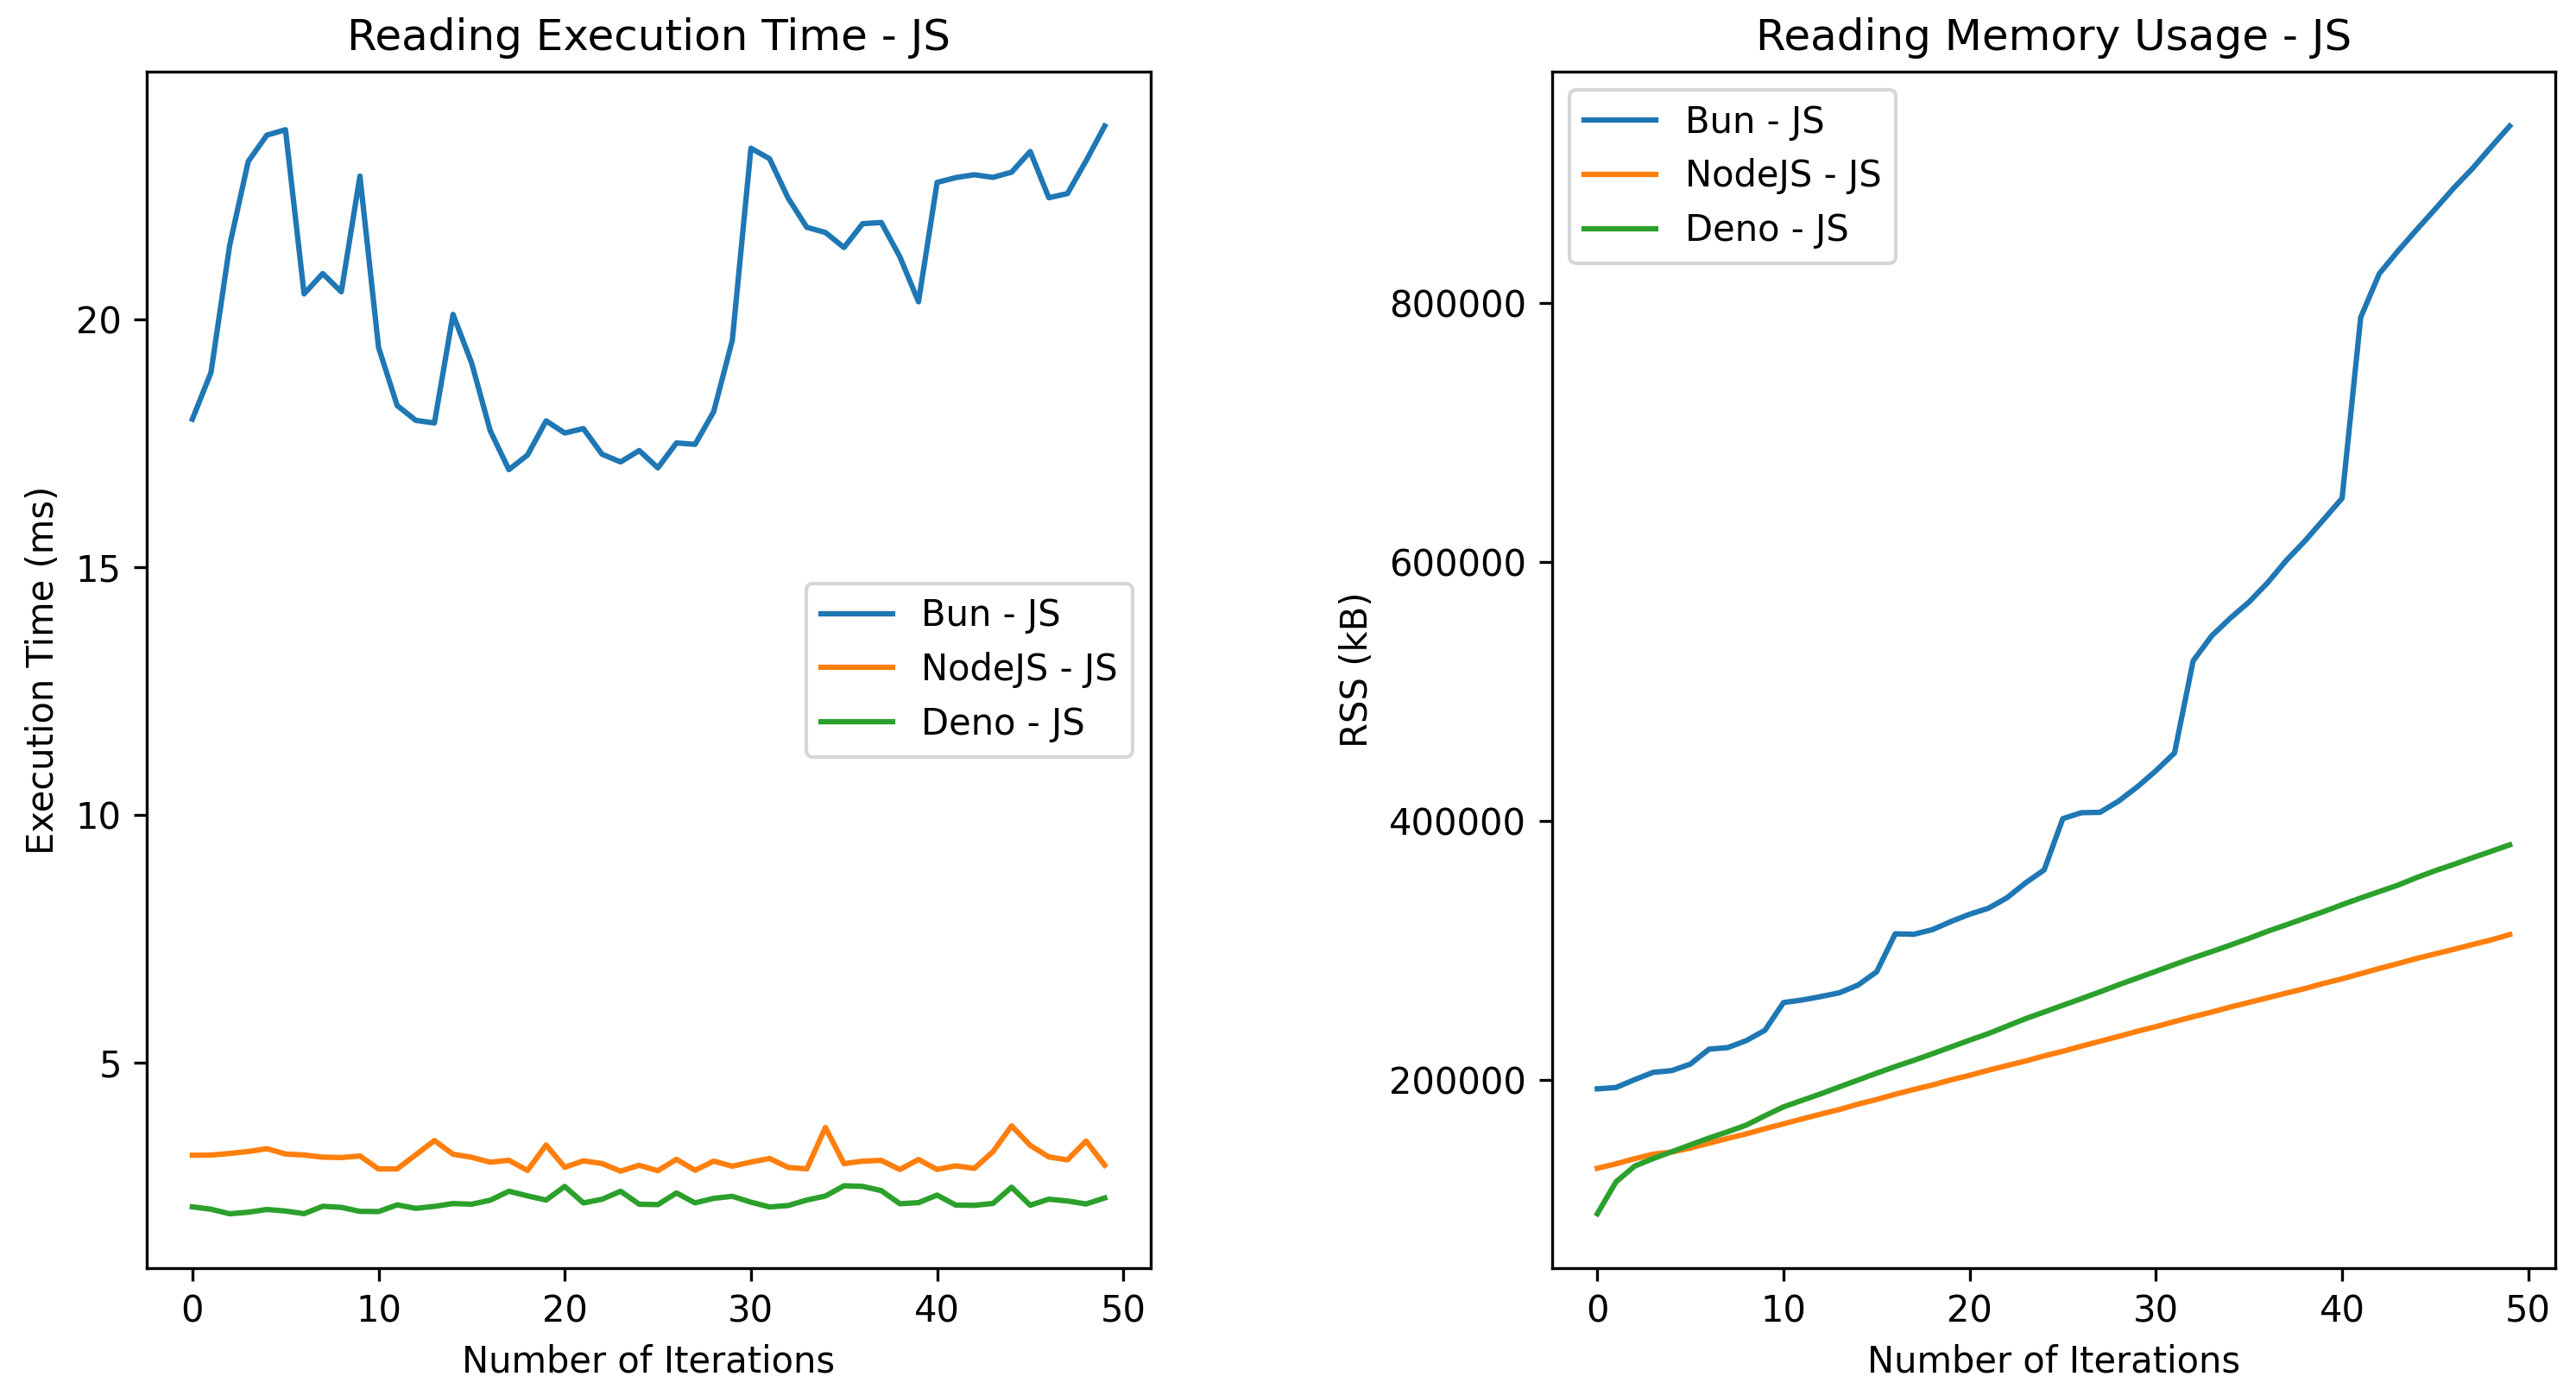
\includegraphics[width=0.68\textwidth]{Figures/files/files_writing_50_2000_50_js.png}
  \caption{Wynik eksperymentów zapisu pliku dla 50 iteracji oraz 50 plików o rozmiarze 1MB - po lewej czas wykonania jednorazowego testu w milisekundach, po prawej ilość zajmowanej pamięci w kilobajtach (kB)}
  \label{fig:file_e2_reading_js}
\end{figure}

Na rysunku \ref{fig:file_e2_writing_js} przedstawiono wyniki eksperymentów dla operacji odczytu dla 50 iteracji oraz 50 plików o rozmiarze 1MB napisanego w języku JavaScript. Na wykresie przedstawiono czas wykonania jednorazowego testu w milisekundach oraz ilość zajmowanej pamięci w kilobajtach (kB).

\begin{figure}[H]
  \centering
  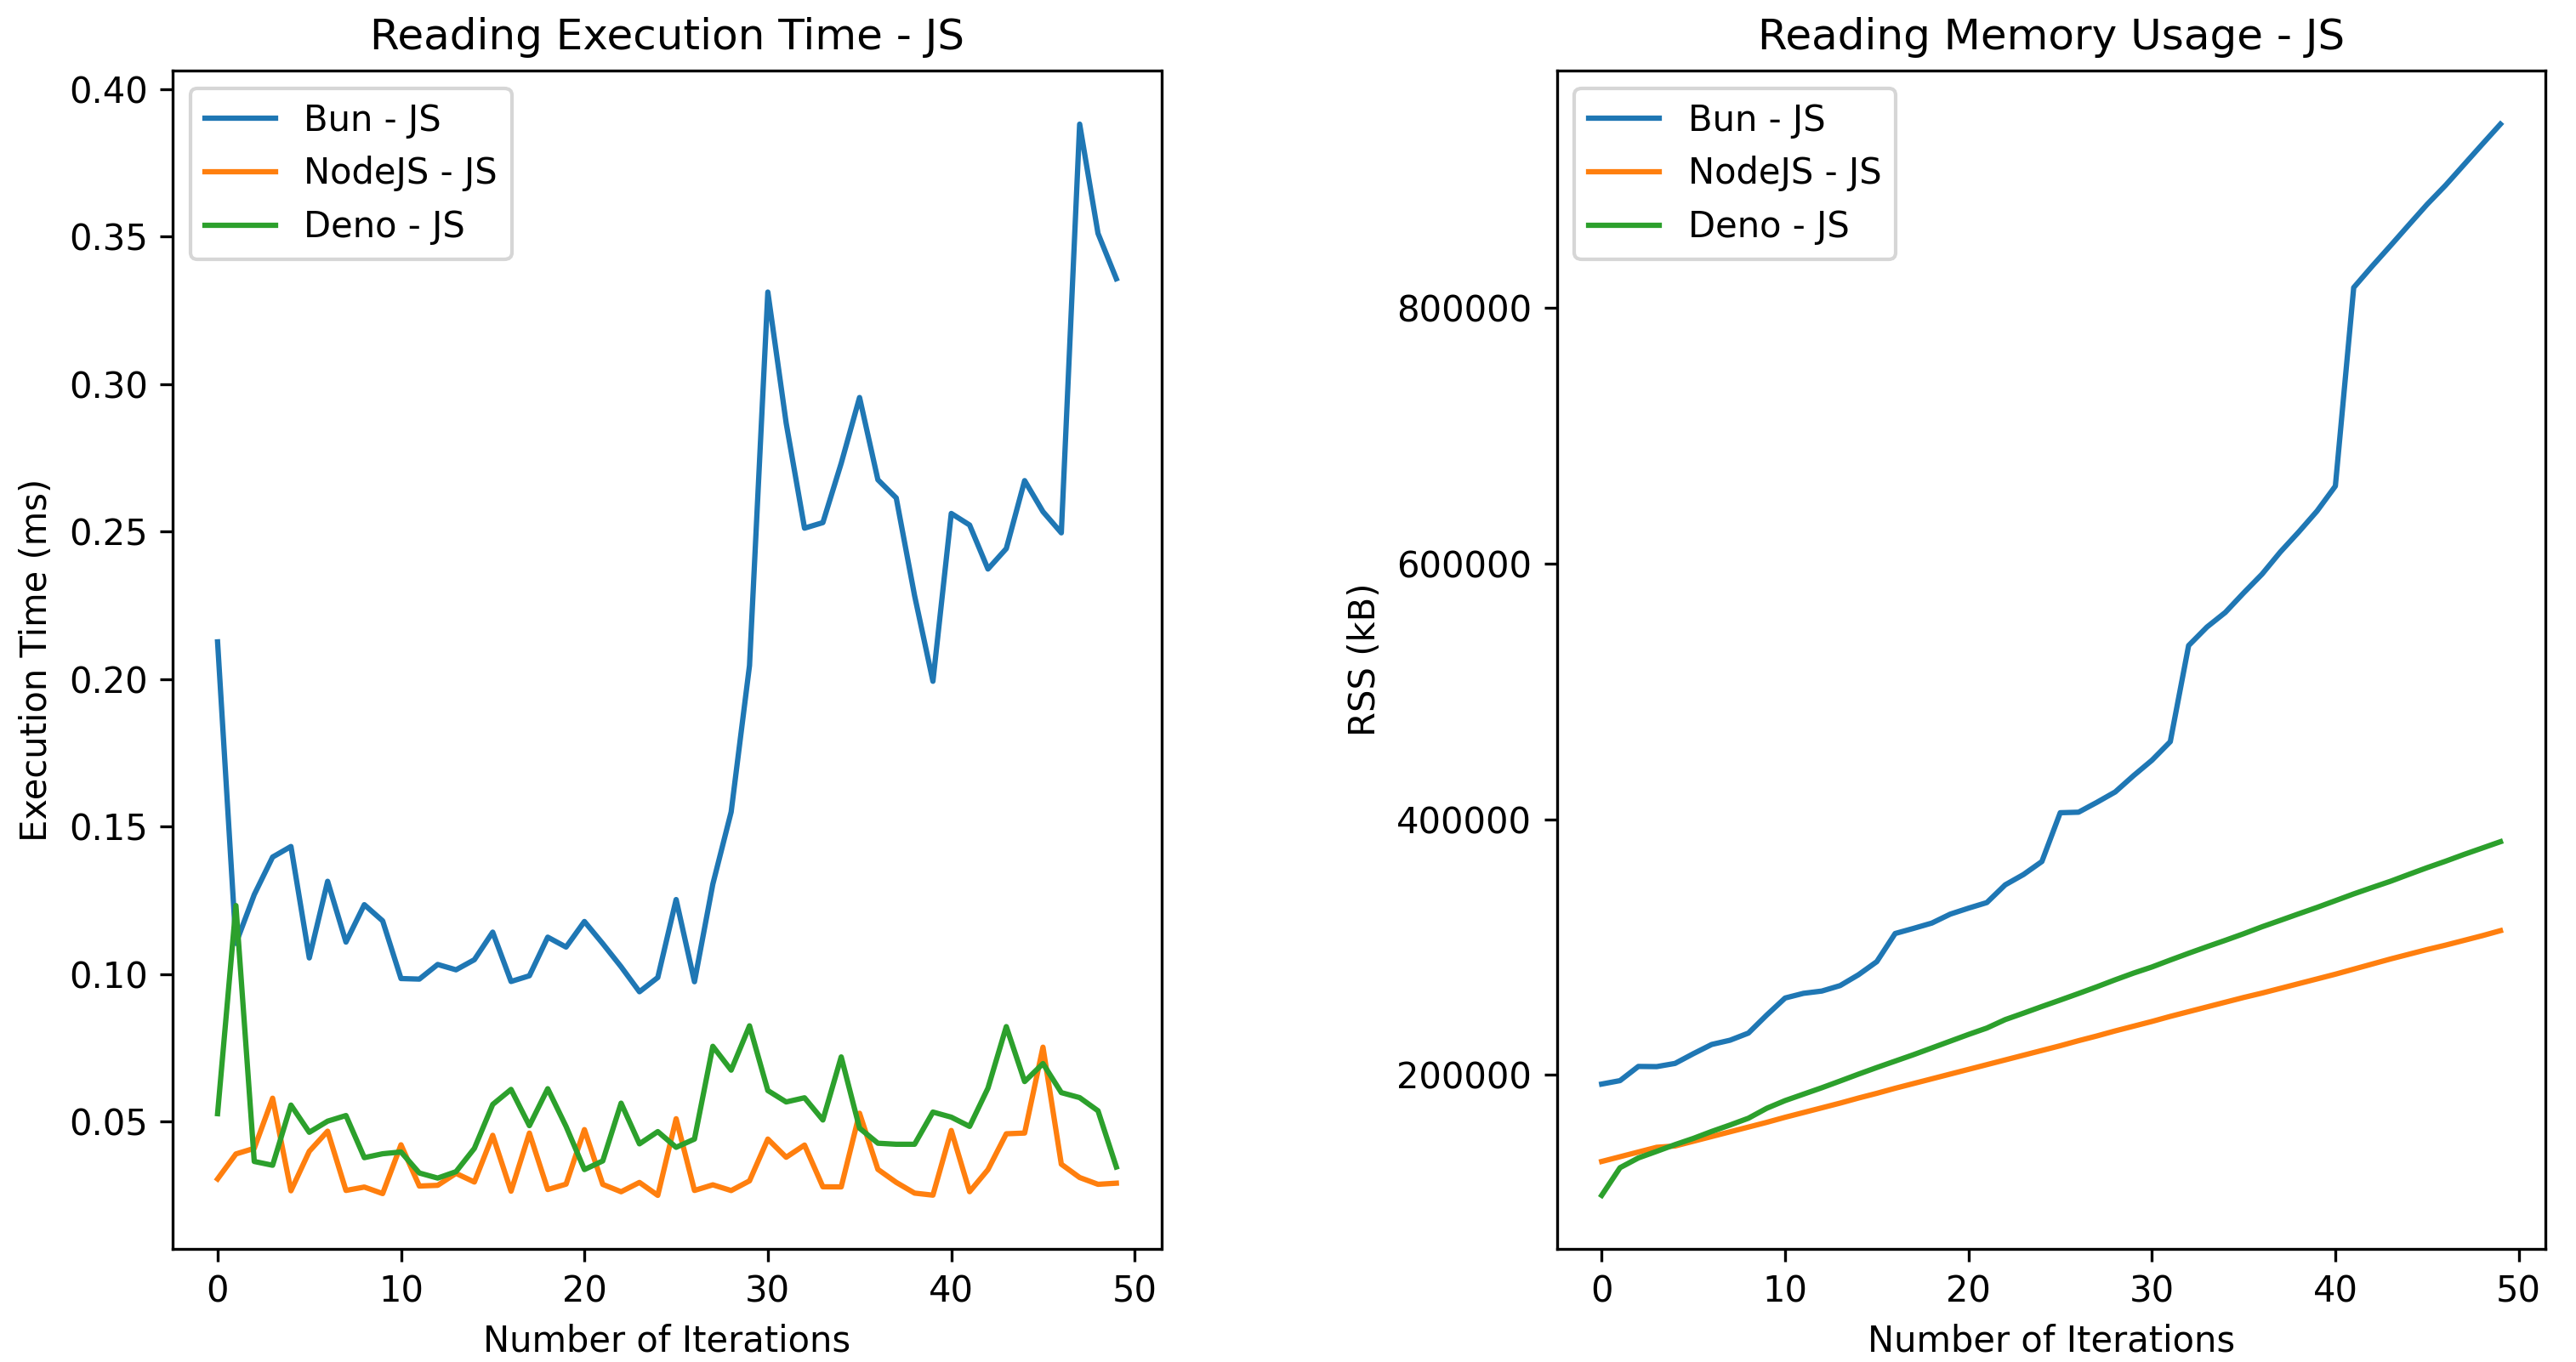
\includegraphics[width=0.68\textwidth]{Figures/files/files_reading_50_2000_50_js.png}
  \caption{Wynik eksperymentów odczytu pliku dla 50 iteracji oraz 50 plików o rozmiarze 1MB - po lewej czas wykonania jednorazowego testu w milisekundach, po prawej ilość zajmowanej pamięci w kilobajtach (kB)}
  \label{fig:file_e2_writing_js}
\end{figure}

Na rysunku \ref{fig:file_e2_reading_ts} przedstawiono wyniki eksperymentów dla operacji zapisu dla 50 iteracji oraz 50 plików o rozmiarze 1MB napisanego w języku TypeScript. Na wykresie przedstawiono czas wykonania jednorazowego testu w milisekundach oraz ilość zajmowanej pamięci w kilobajtach (kB).

\begin{figure}[H]
  \centering
  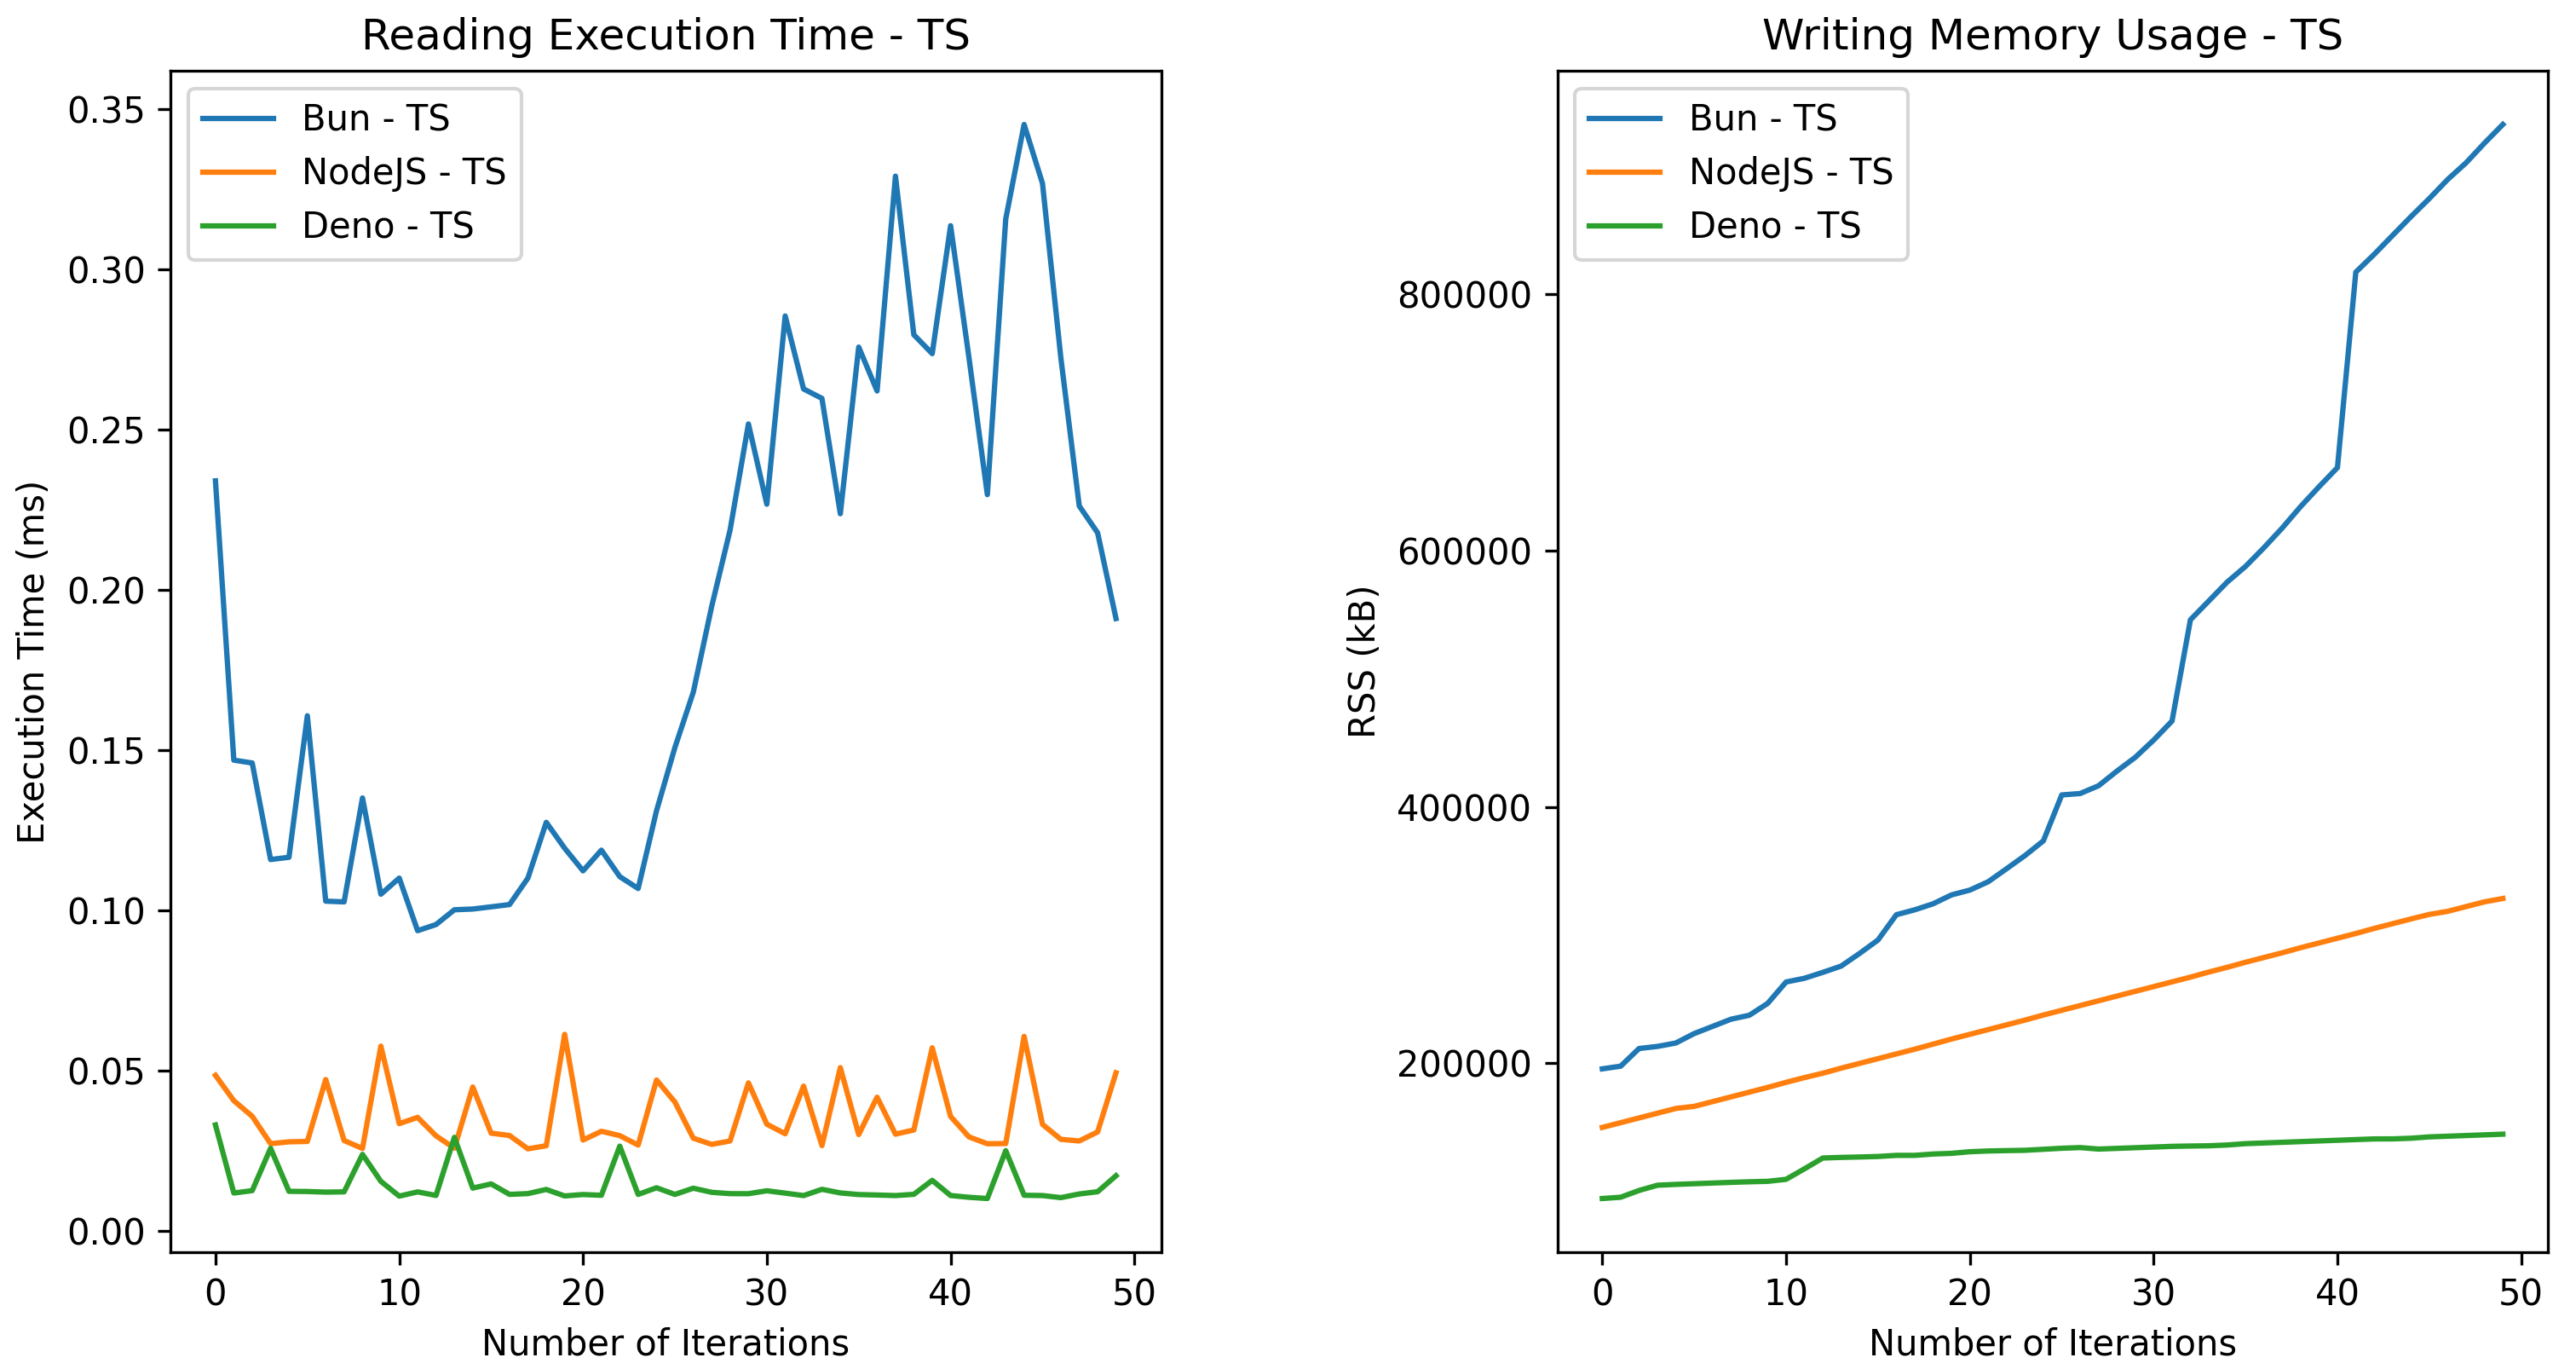
\includegraphics[width=0.68\textwidth]{Figures/files/files_reading_50_2000_50_ts.png}
  \caption{Wynik eksperymentów zapisu pliku dla 50 iteracji oraz 50 plików o rozmiarze 1MB - po lewej czas wykonania jednorazowego testu w milisekundach, po prawej ilość zajmowanej pamięci w kilobajtach (kB)}
  \label{fig:file_e2_reading_ts}
\end{figure}

Na rysunku \ref{fig:file_e2_writing_ts} przedstawiono wyniki eksperymentów dla operacji odczytu dla 50 iteracji oraz 50 plików o rozmiarze 1MB napisanego w języku TypeScript. Na wykresie przedstawiono czas wykonania jednorazowego testu w milisekundach oraz ilość zajmowanej pamięci w kilobajtach (kB).

\begin{figure}[H]
  \centering
  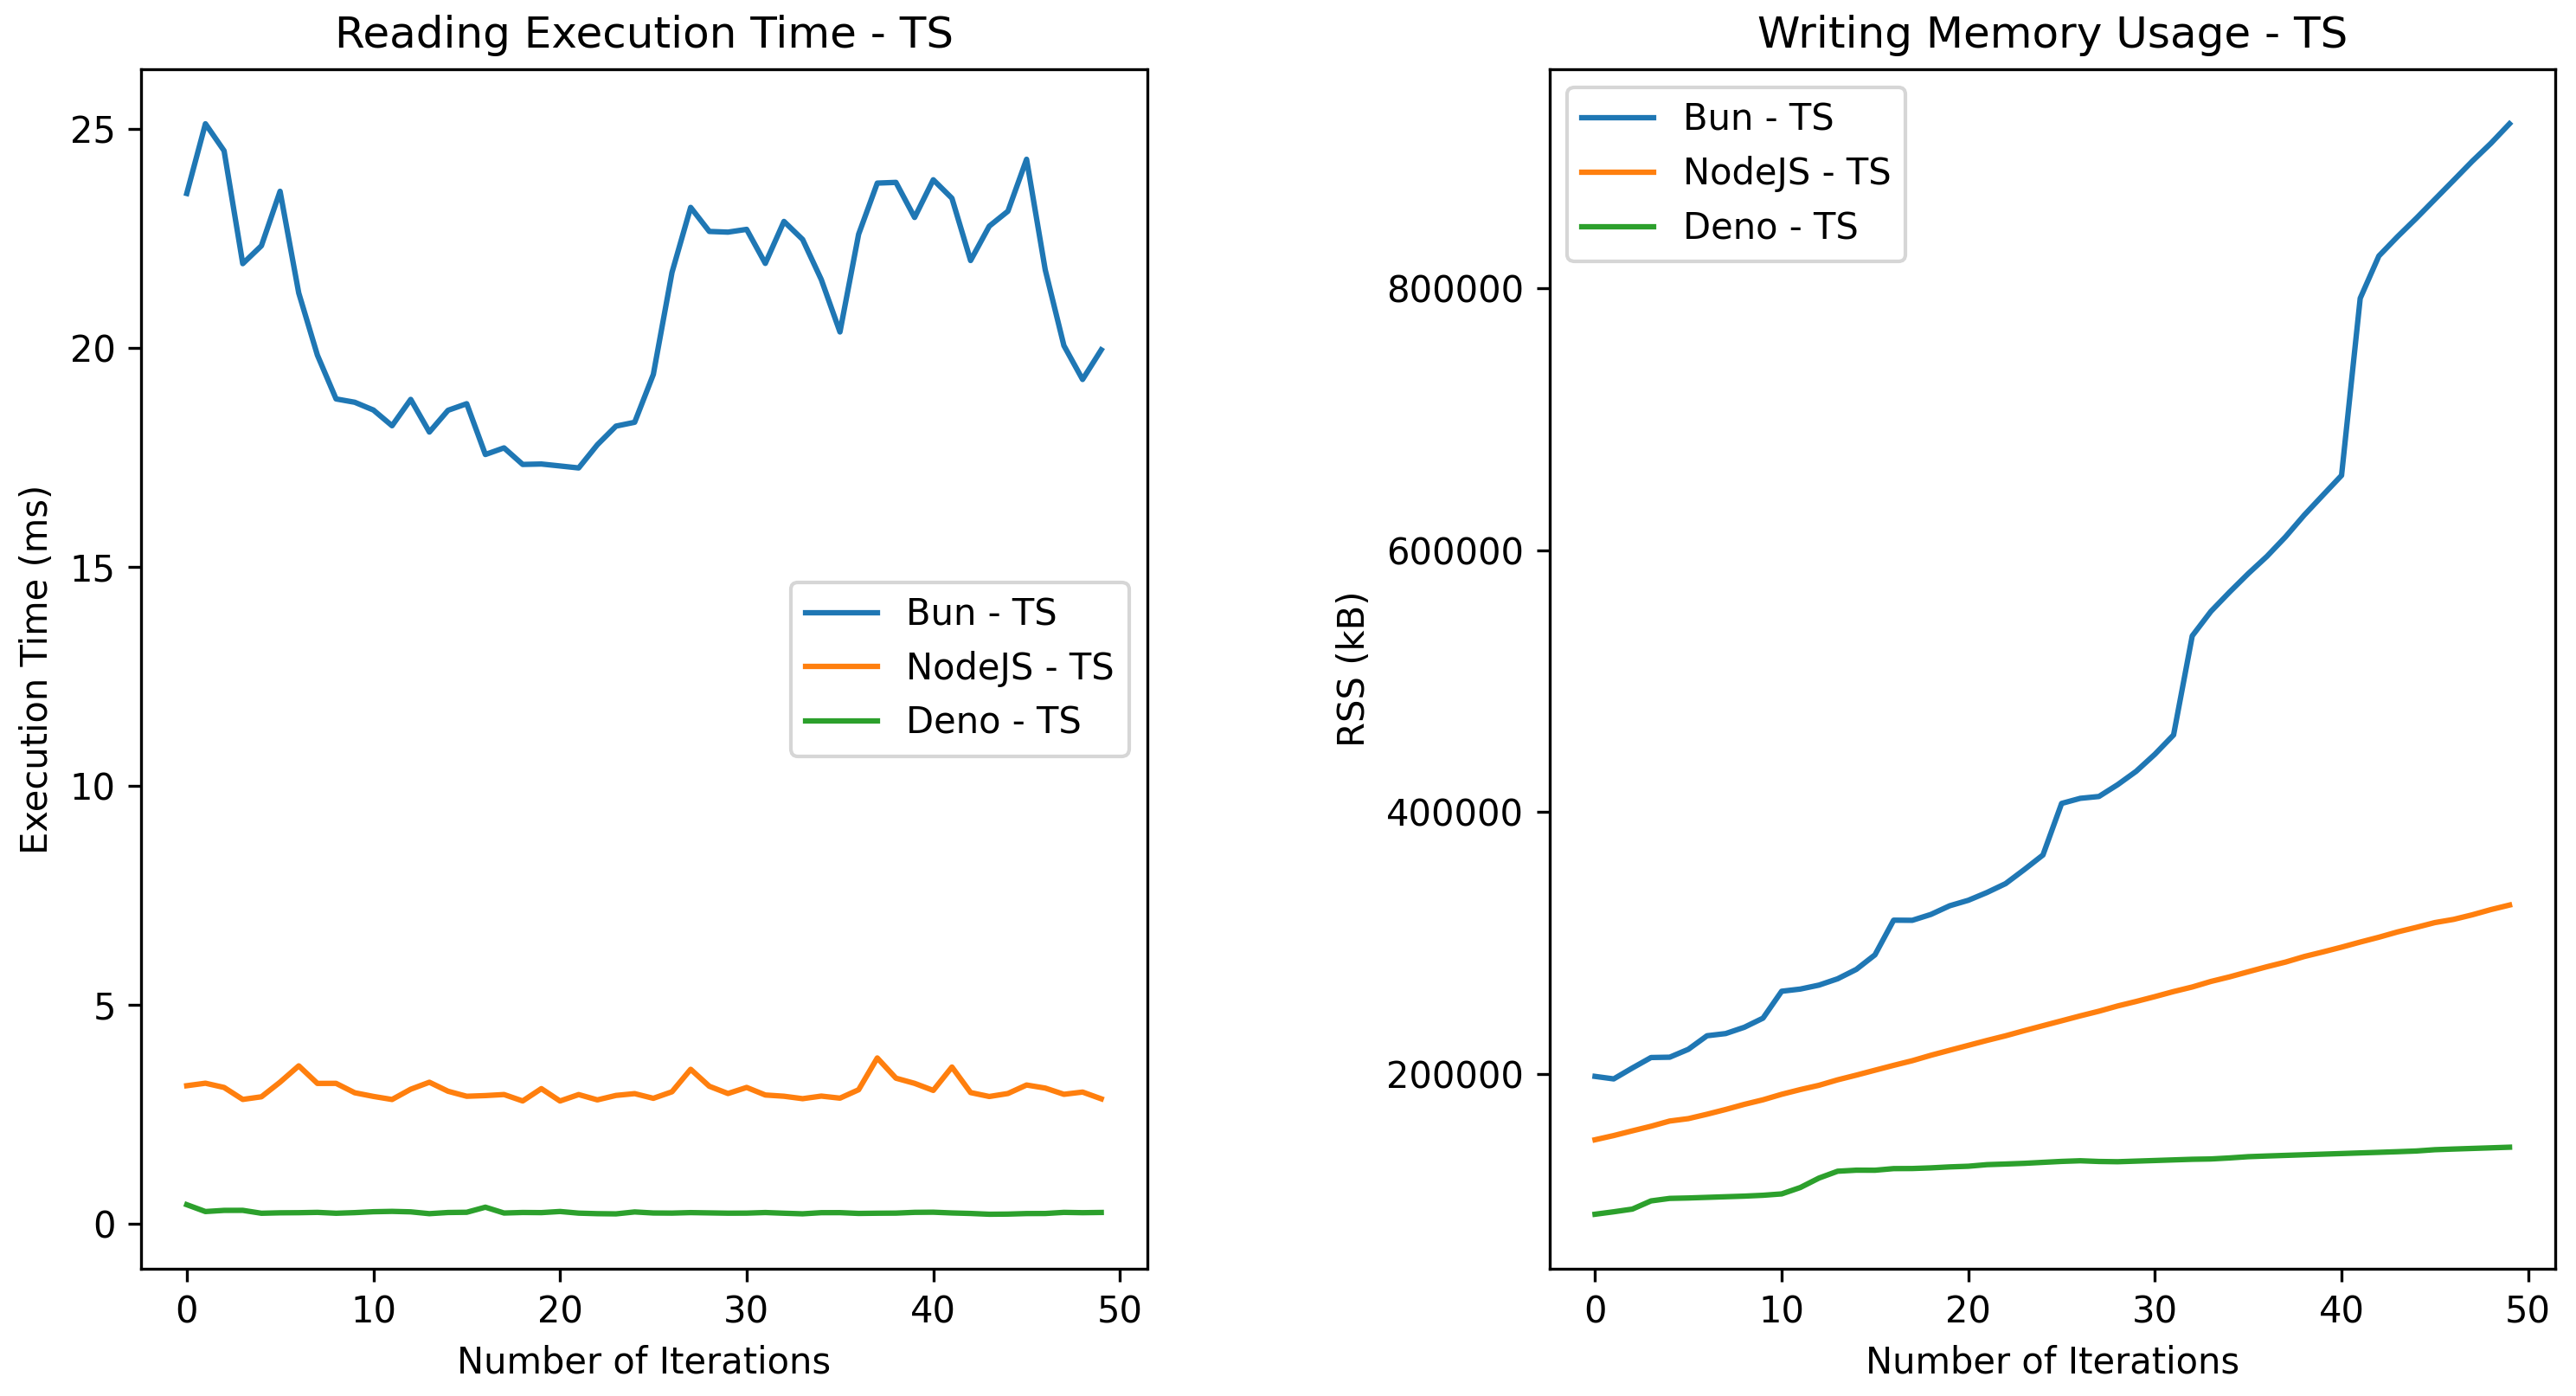
\includegraphics[width=0.68\textwidth]{Figures/files/files_writing_50_2000_50_ts.png}
  \caption{Wynik eksperymentów zapisu pliku dla 50 iteracji oraz 50 plików o rozmiarze 1MB - po lewej czas wykonania jednorazowego testu w milisekundach, po prawej ilość zajmowanej pamięci w kilobajtach (kB)}
  \label{fig:file_e2_writing_ts}
\end{figure}

\subsection{Testy wydajnościowe serwera HTTP}
W celu zbadania wydajności serwera HTTP, przeprowadzono testy obciążeniowe. Do testów została wykorzystany program \textit{oha} \cite{oha}, który pozwala na połączenie się do serwera HTTP oraz wysyłanie żądań z kilku połączeń jednocześnie. W tabeli \ref{tab:http_experiments} przedstawiono liczbę przeprowadzonych eksperymentów oraz ilość połączeń.

\begin{table}[H]
  \centering
  \caption{Parametry eksperymentów serwera HTTP}
  \begin{tabular}{|c|c|}
    \hline
    \textbf{Liczba żądań} & \textbf{Ilość połączeń}\\ \hline
    10000 & 100 \\ \hline
    10000 & 1000 \\ \hline
    10000 & 10000 \\ \hline
  \end{tabular}
  \label{tab:http_experiments}
\end{table}

\subsubsection{Wyniki}
Na rysunku \ref{fig:server_e1} przedstawiono wyniki eksperymentów dla testu wydajnościowego serwera HTTP dla 100 równoczesnych połączeń oraz 10000 żądań HTTP. Wyniki zostały przedstawione zarówno dla języka JavaScript oraz TypeScript. Na wykresie przedstawiono wynik testu obciążeniowego wyrażonego w RPS (\textit{Request per second}).

\begin{figure}[H]
  \centering
  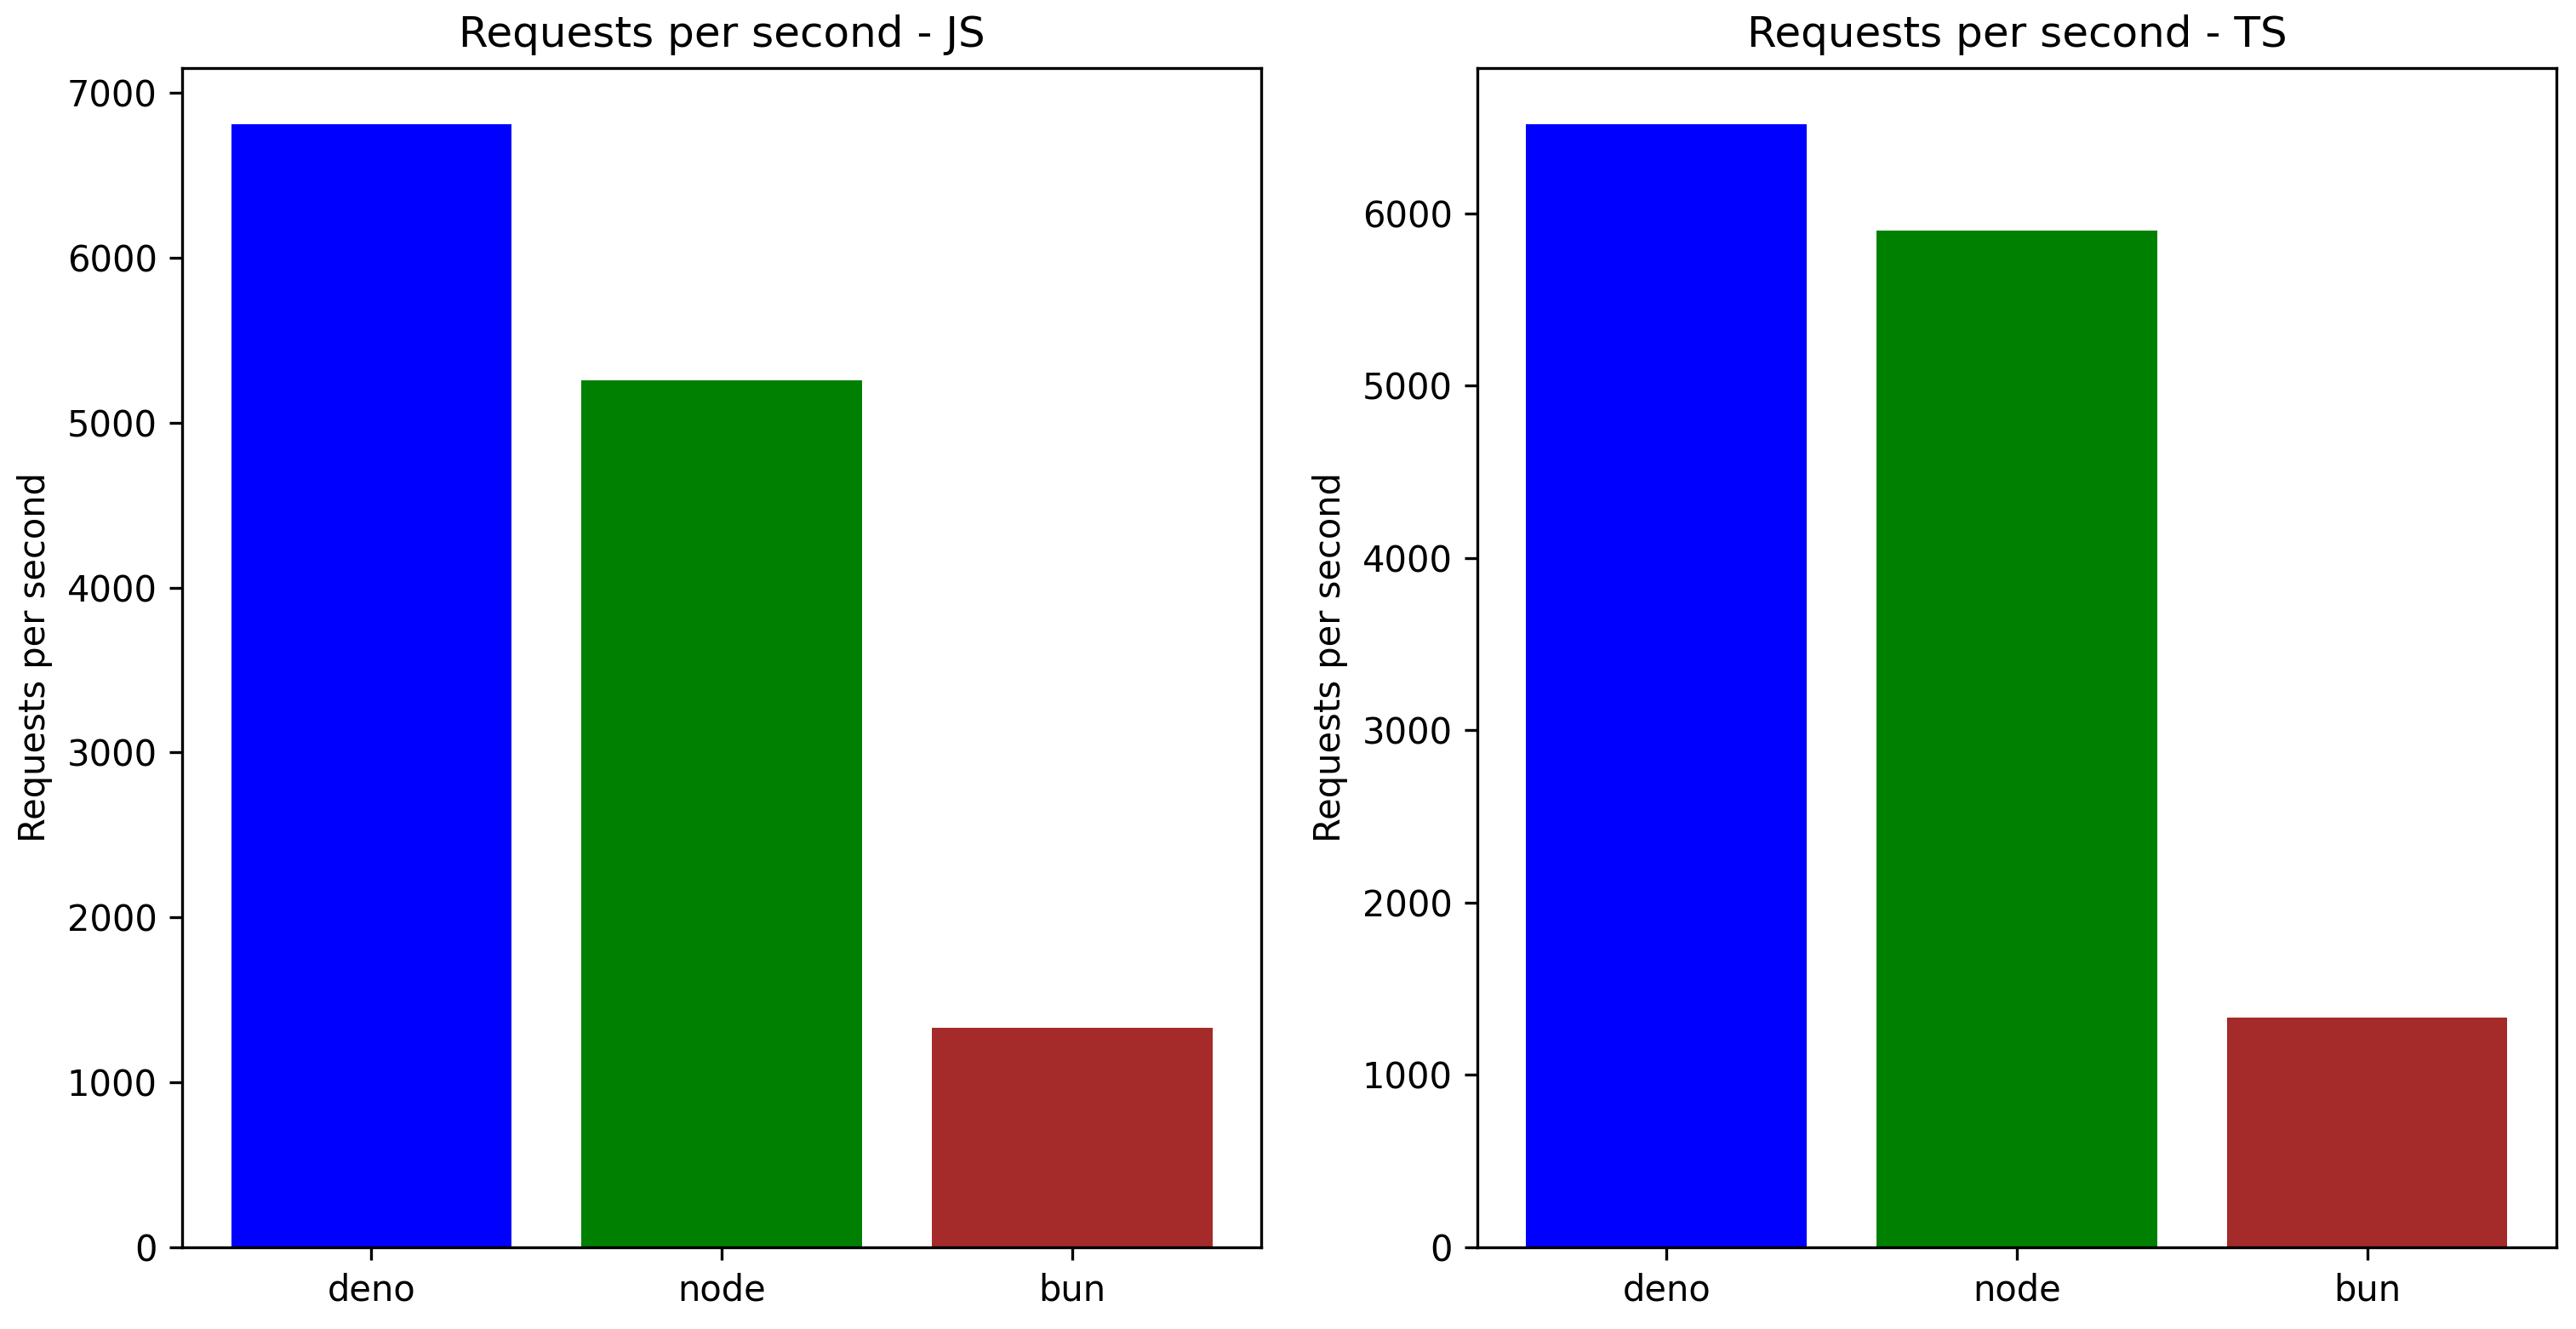
\includegraphics[width=0.68\textwidth]{Figures/server/server_100_10000.png}
  \caption{Wynik eksperymentów dla testu serwera HTTP 100 równoczesnych połączeń oraz 10000 żądań HTTP - wykres przedstawia wynik testu obciążeniowego wyrażonego w RPS (\textit{Request per second})}
  \label{fig:server_e1}
\end{figure}

Na rysunku \ref{fig:server_e2} przedstawiono wyniki eksperymentów dla testu wydajnościowego serwera HTTP dla 1000 równoczesnych połączeń oraz 10000 żądań HTTP. Wyniki zostały przedstawione zarówno dla języka JavaScript oraz TypeScript. Na wykresie przedstawiono wynik testu obciążeniowego wyrażonego w RPS (\textit{Request per second}).

\begin{figure}[H]
  \centering
  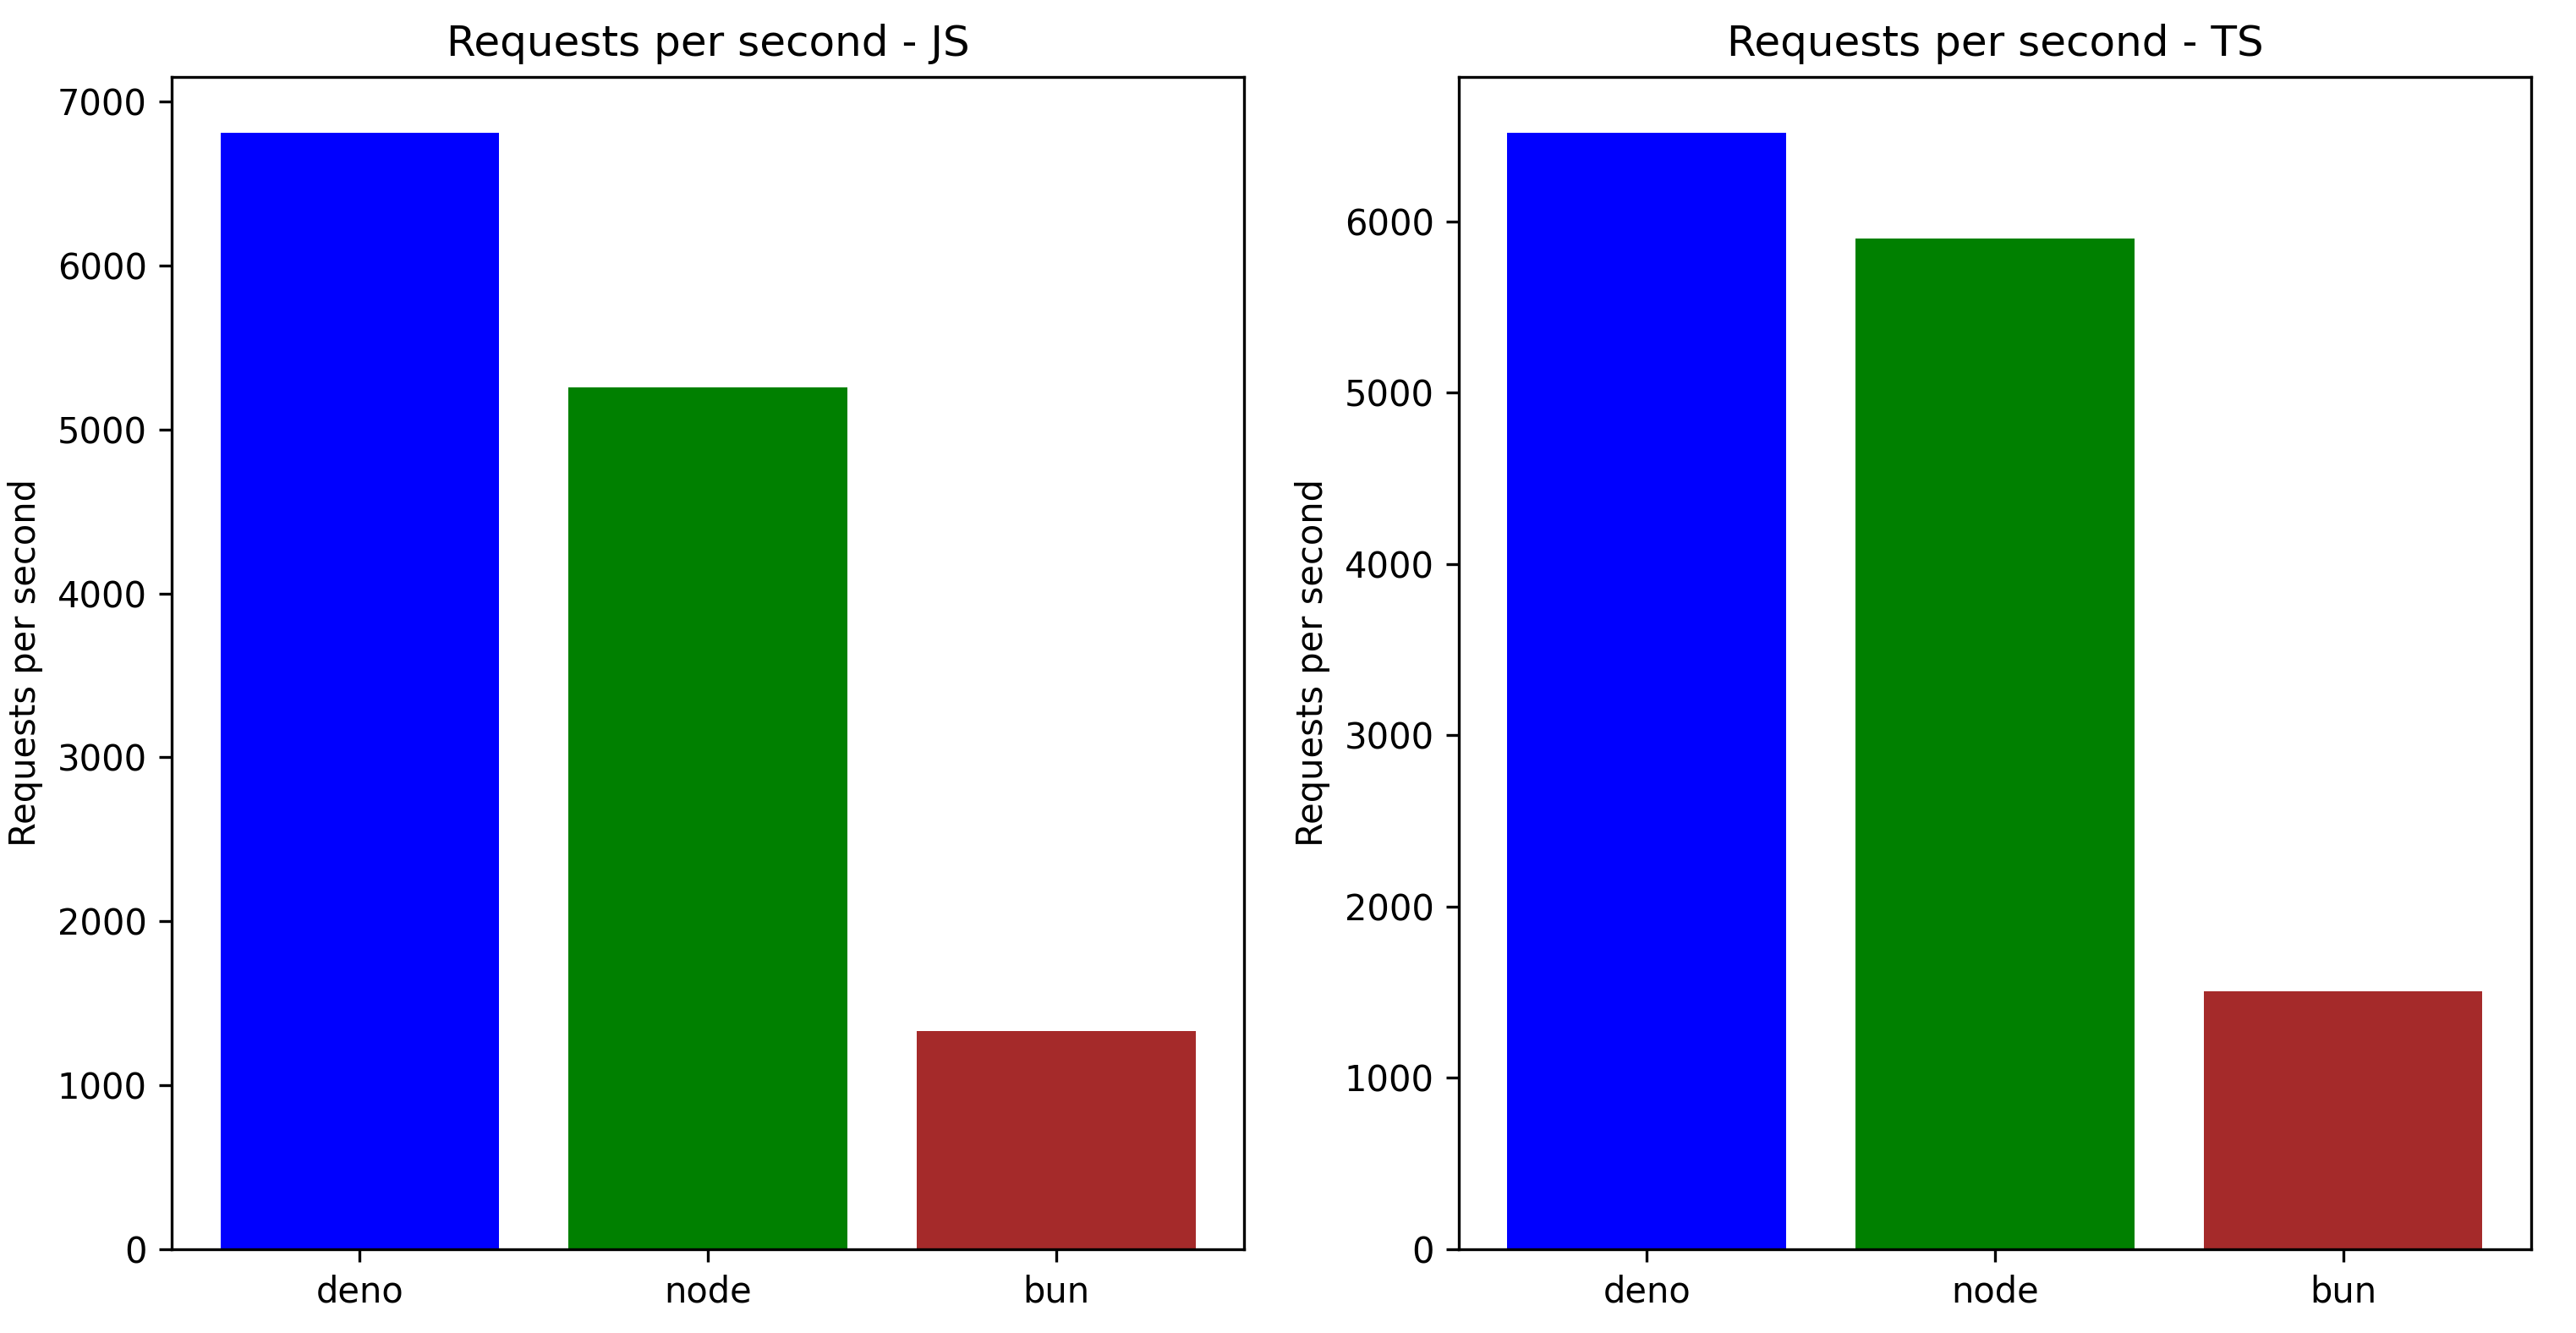
\includegraphics[width=0.68\textwidth]{Figures/server/server_1000_10000.png}
  \caption{Wynik eksperymentów dla testu serwera HTTP 1000 równoczesnych połączeń oraz 10000 żądań HTTP - wykres przedstawia wynik testu obciążeniowego wyrażonego w RPS (\textit{Request per second})}
  \label{fig:server_e2}
\end{figure}

Na rysunku \ref{fig:server_e3} przedstawiono wyniki eksperymentów dla testu wydajnościowego serwera HTTP dla 10000 równoczesnych połączeń oraz 10000 żądań HTTP. Wyniki zostały przedstawione zarówno dla języka JavaScript oraz TypeScript. Na wykresie przedstawiono wynik testu obciążeniowego wyrażonego w RPS (\textit{Request per second}).

\begin{figure}[H]
  \centering
  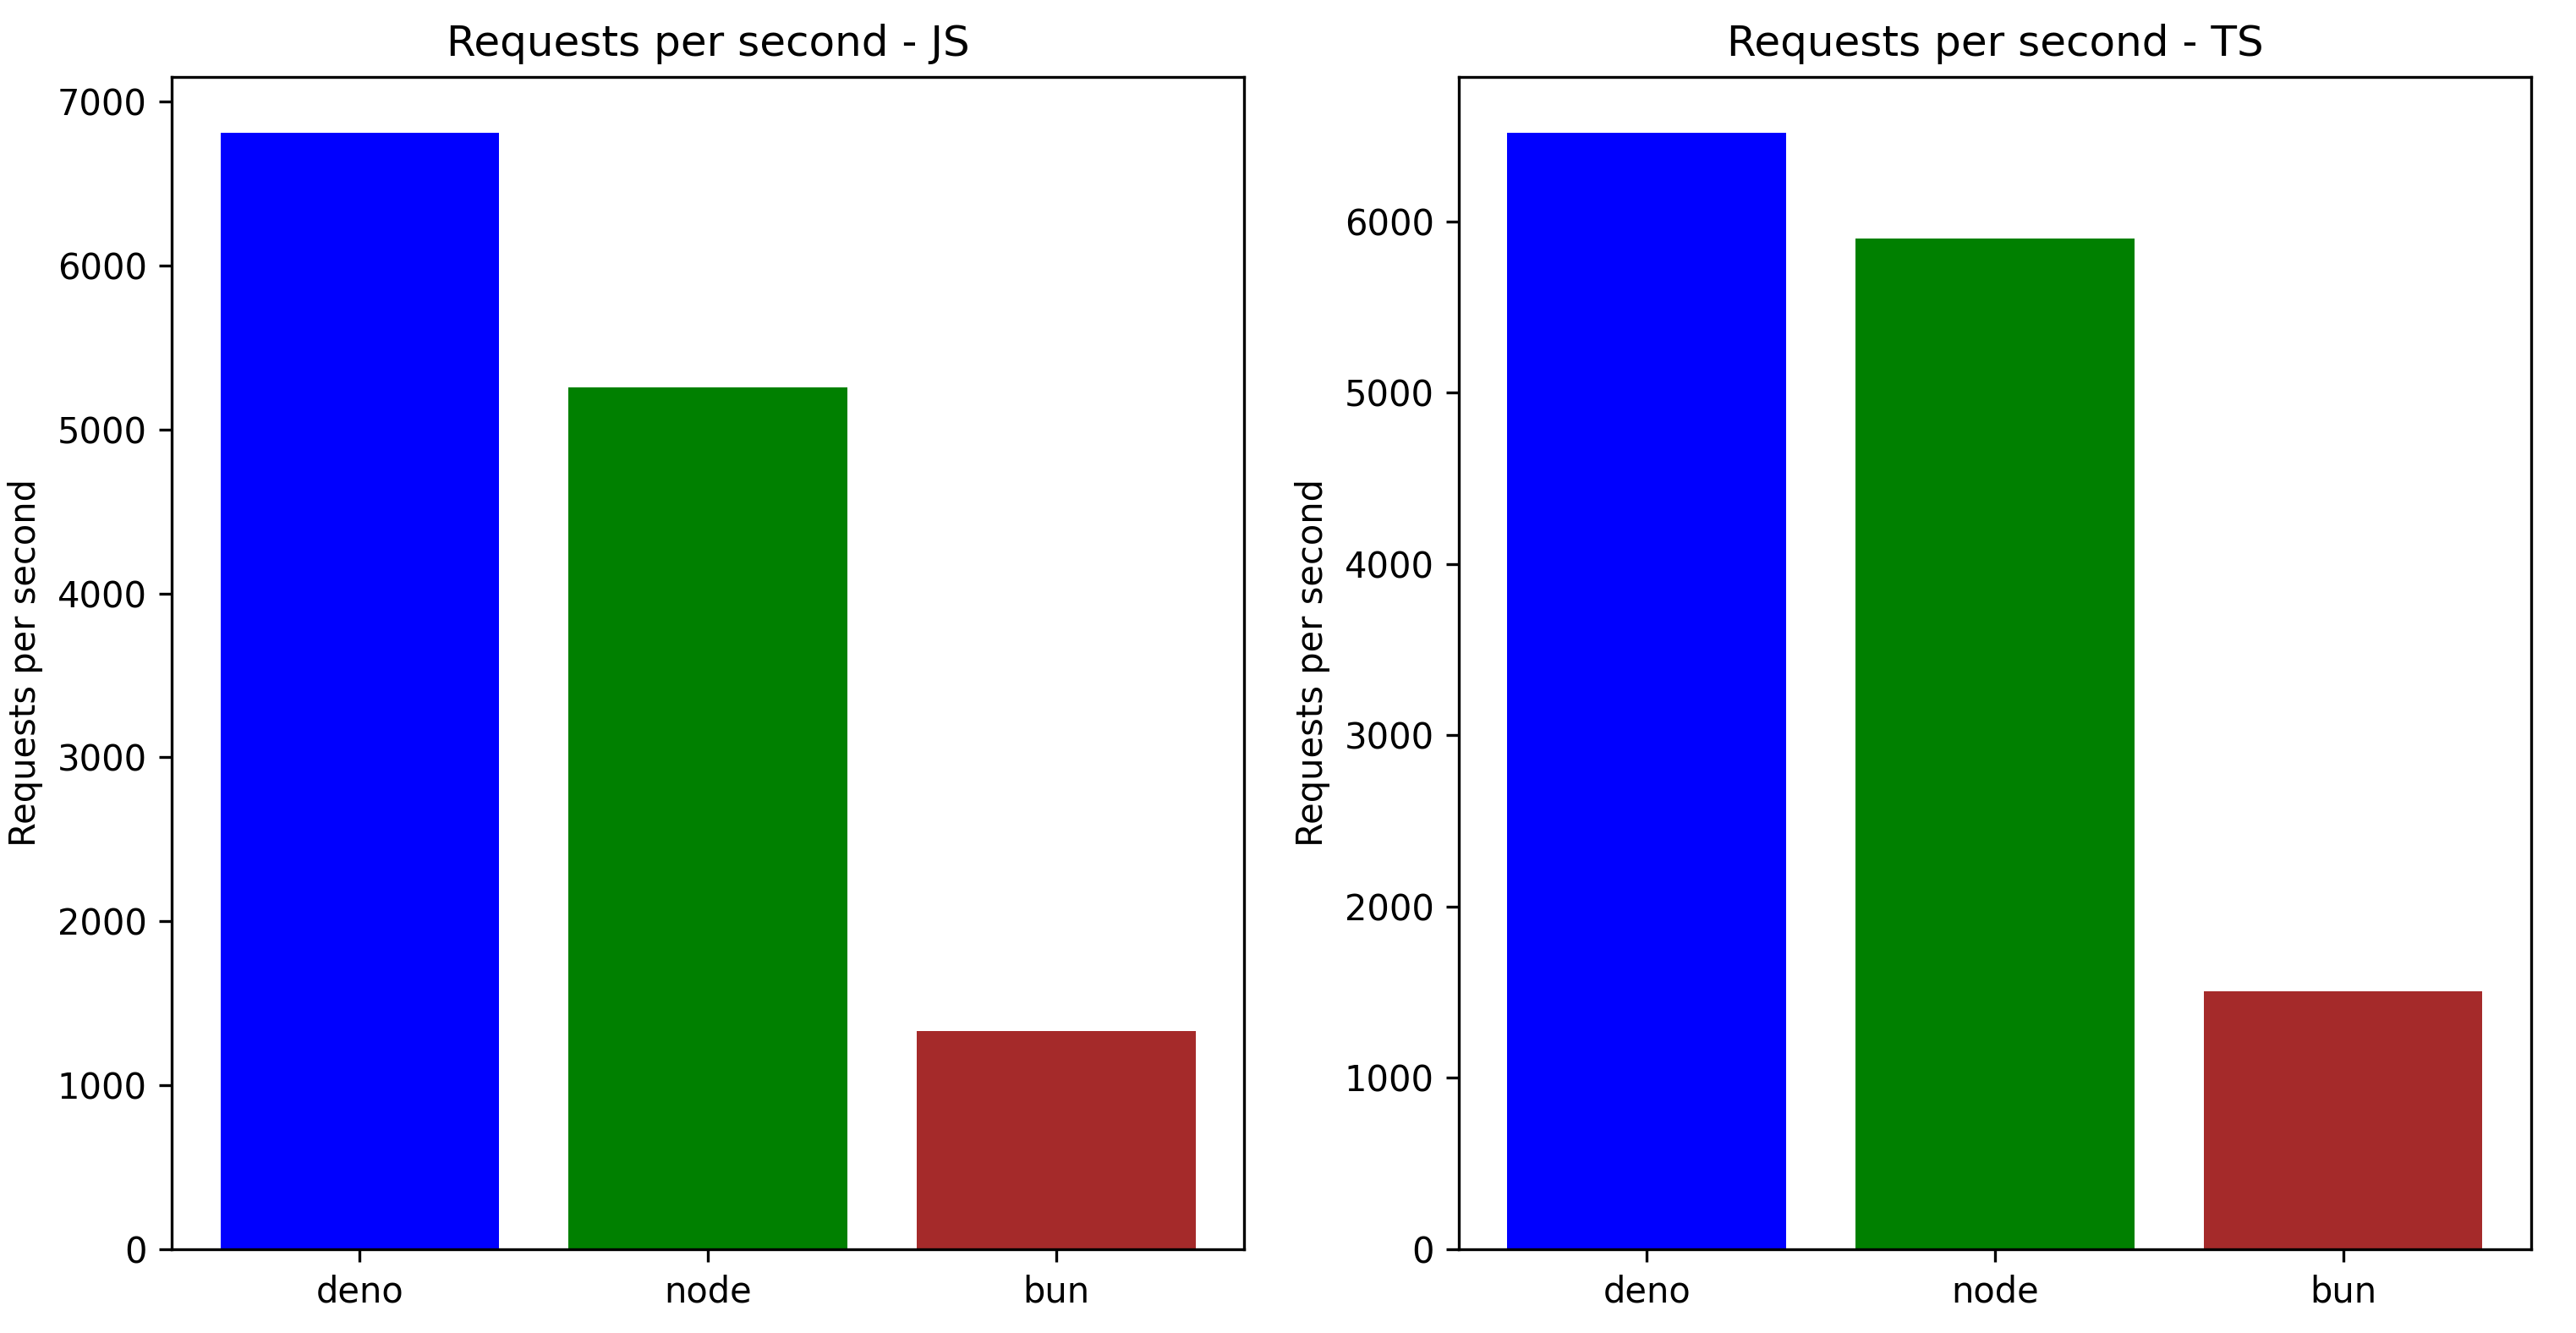
\includegraphics[width=0.68\textwidth]{Figures/server/server_1000_10000.png}
  \caption{Wynik eksperymentów dla testu serwera HTTP 10000 równoczesnych połączeń oraz 10000 żądań HTTP - wykres przedstawia wynik testu obciążeniowego wyrażonego w RPS (\textit{Request per second})}
  \label{fig:server_e3}
\end{figure}

\subsection{Testy wydajnościowe zapisu i odczytu danych z bazy danych}
W celu zbadania wydajności operacji zapisu oraz odczytu danych z bazy danych, przeprowadzono testy wydajnościowe z wykorzystaniem bazy danych SQLite. W celu wygenerowania danych do bazy danych, wykorzystano moduł \textit{faker.js}. W tabeli \ref{tab:database_experiments} przedstawiono liczbę przeprowadzonych eksperymentów oraz ilość rekordów.

\begin{table}[H]
  \centering
  \caption{Parametry eksperymentów zapisu i odczytu danych z bazy danych}
  \begin{tabular}{|c|c|}
    \hline
    \textbf{Liczba eksperymentów} & \textbf{Ilość rekordów}\\ \hline
    10 & 1000 \\ \hline
    100 & 1000 \\ \hline
  \end{tabular}
  \label{tab:database_experiments}
\end{table}

\subsubsection{Wyniki}
Na rysunku \ref{fig:database_e1_js} przedstawiono wyniki eksperymentów dla testu bazy danych dla 10 iteracji oraz 1000 rekordów napisanego w języku JavaScript. Na wykresie przedstawiono czas wykonania jednorazowego testu w milisekundach oraz ilość zajmowanej pamięci w kilobajtach (kB).

\begin{figure}[H]
  \centering
  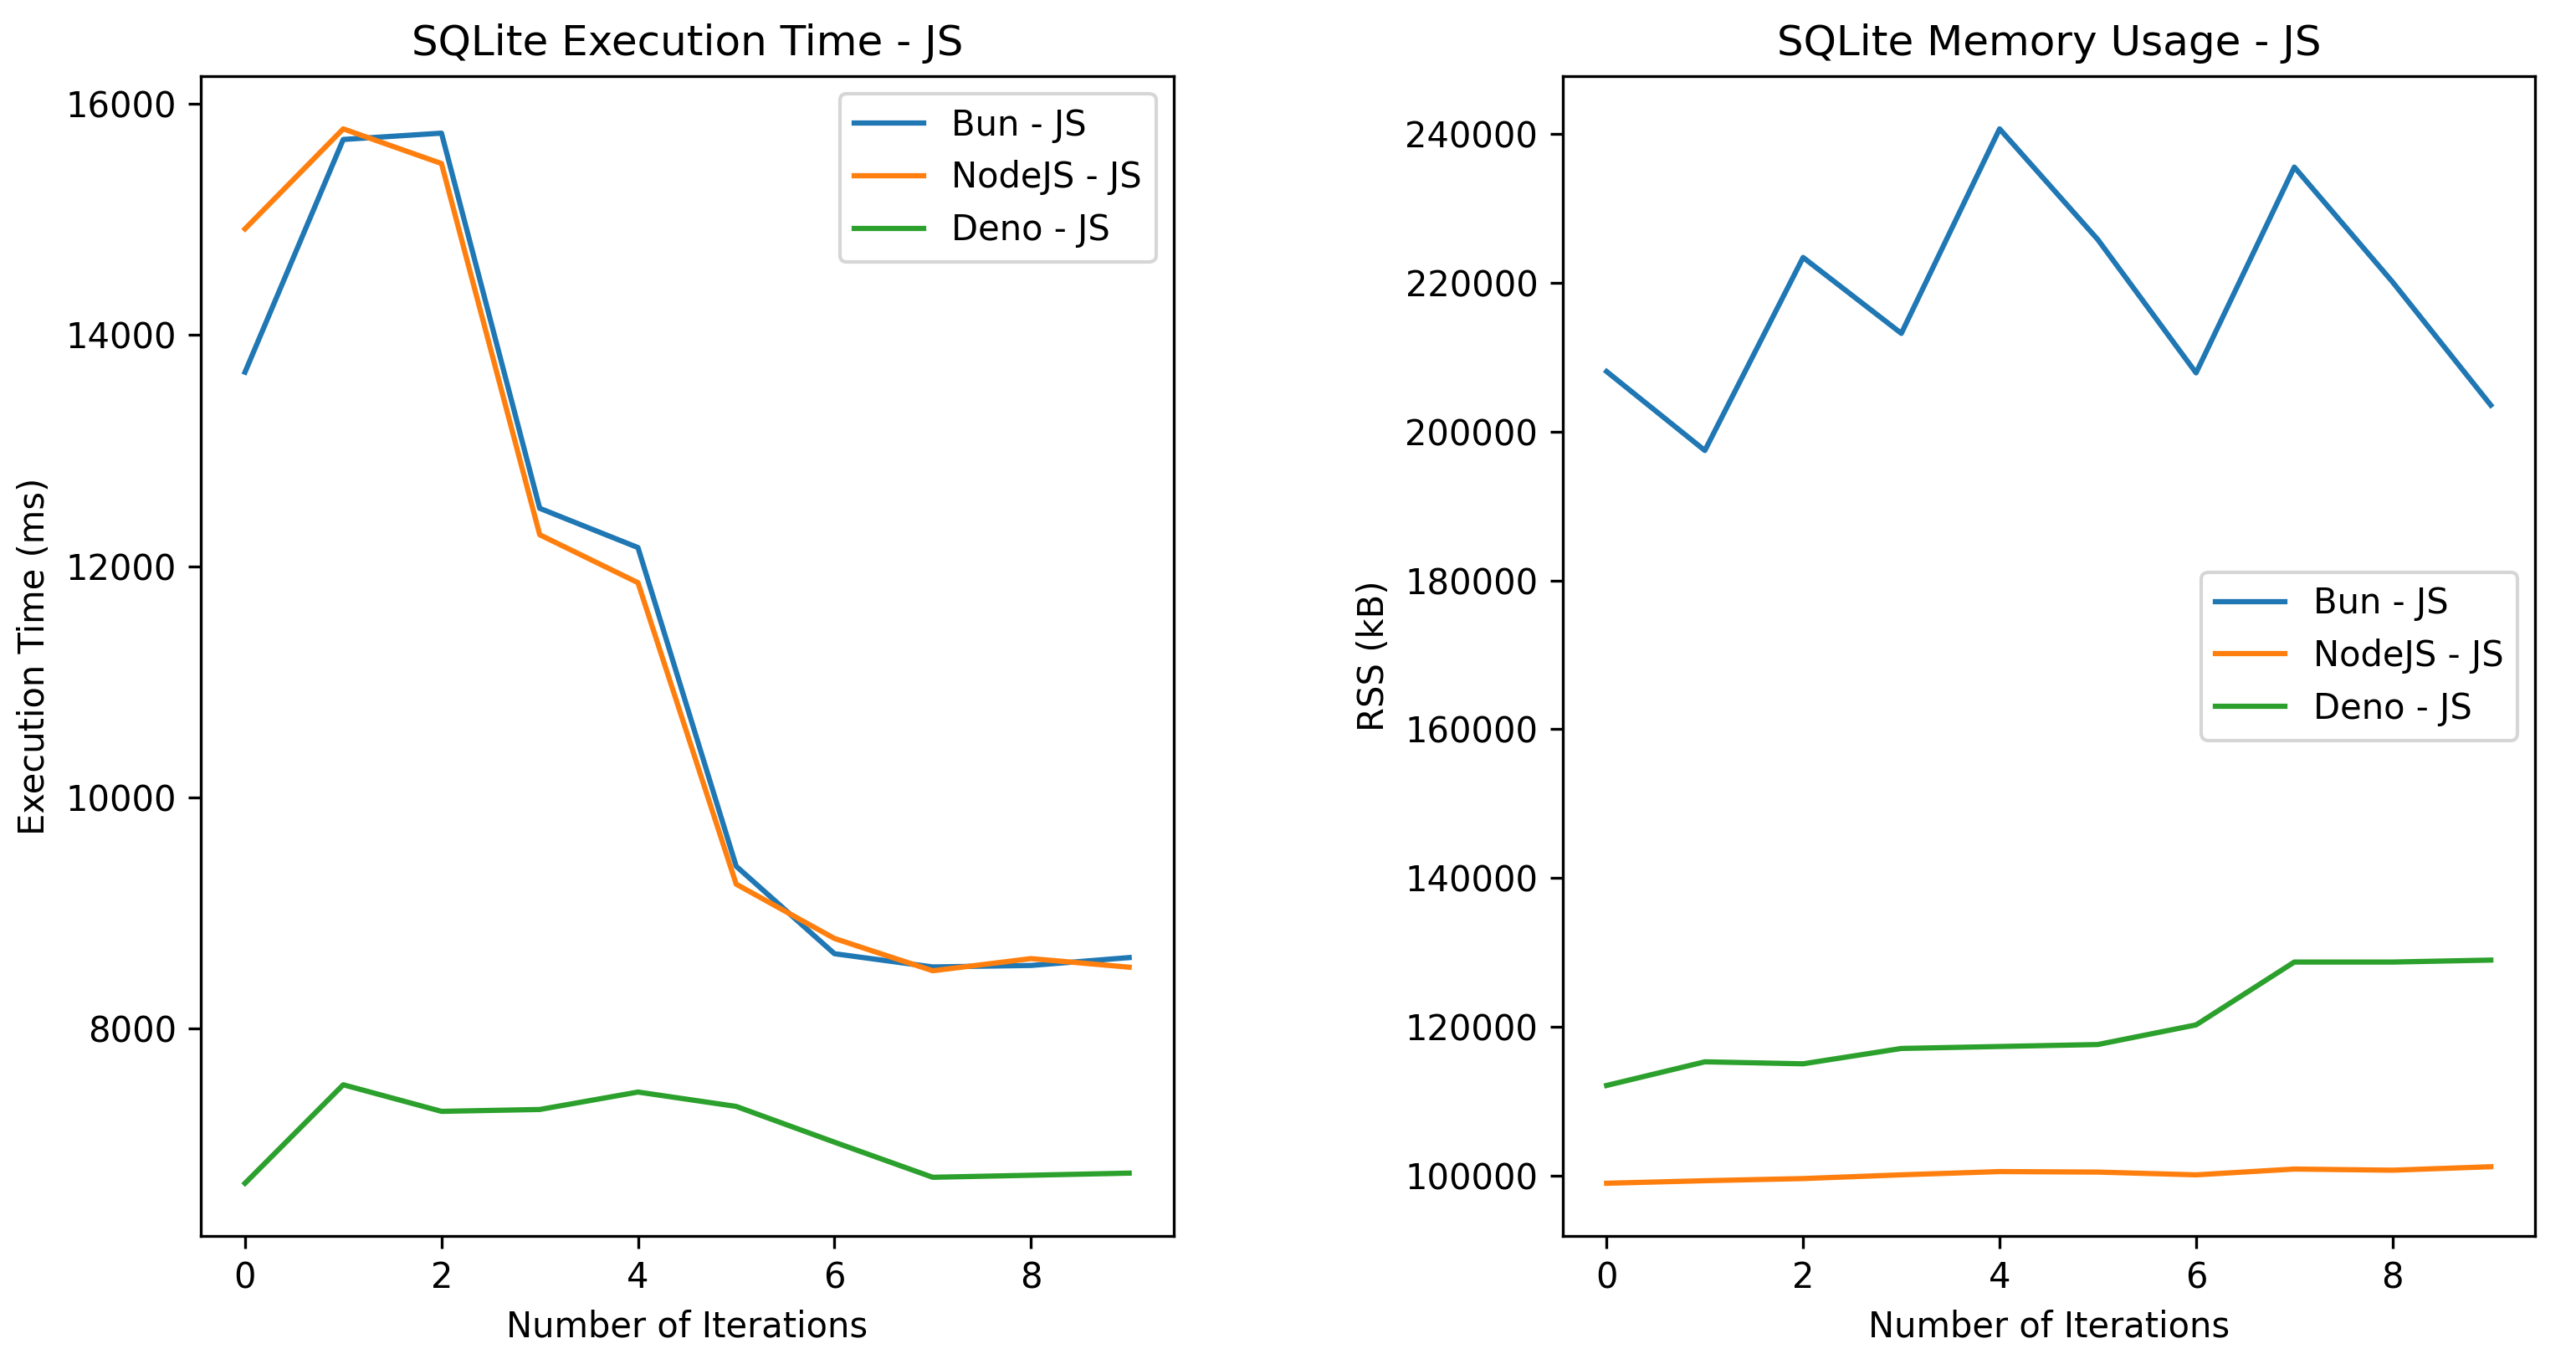
\includegraphics[width=0.68\textwidth]{Figures/database/sqlite_10_1000_js.png}
  \caption{Wyniki eksperymentów dla testu bazy danych 10 iteracji oraz 1000 rekordów - po lewej czas wykonania jednorazowego testu w milisekundach, po prawej ilość zajmowanej pamięci w kilobajtach (kB)}
  \label{fig:database_e1_js}
\end{figure}

Na rysunku \ref{fig:database_e1_ts} przedstawiono wyniki eksperymentów dla testu bazy danych dla 10 iteracji oraz 1000 rekordów napisanego w języku TypeScript. Na wykresie przedstawiono czas wykonania jednorazowego testu w milisekundach oraz ilość zajmowanej pamięci w kilobajtach (kB).

\begin{figure}[H]
  \centering
  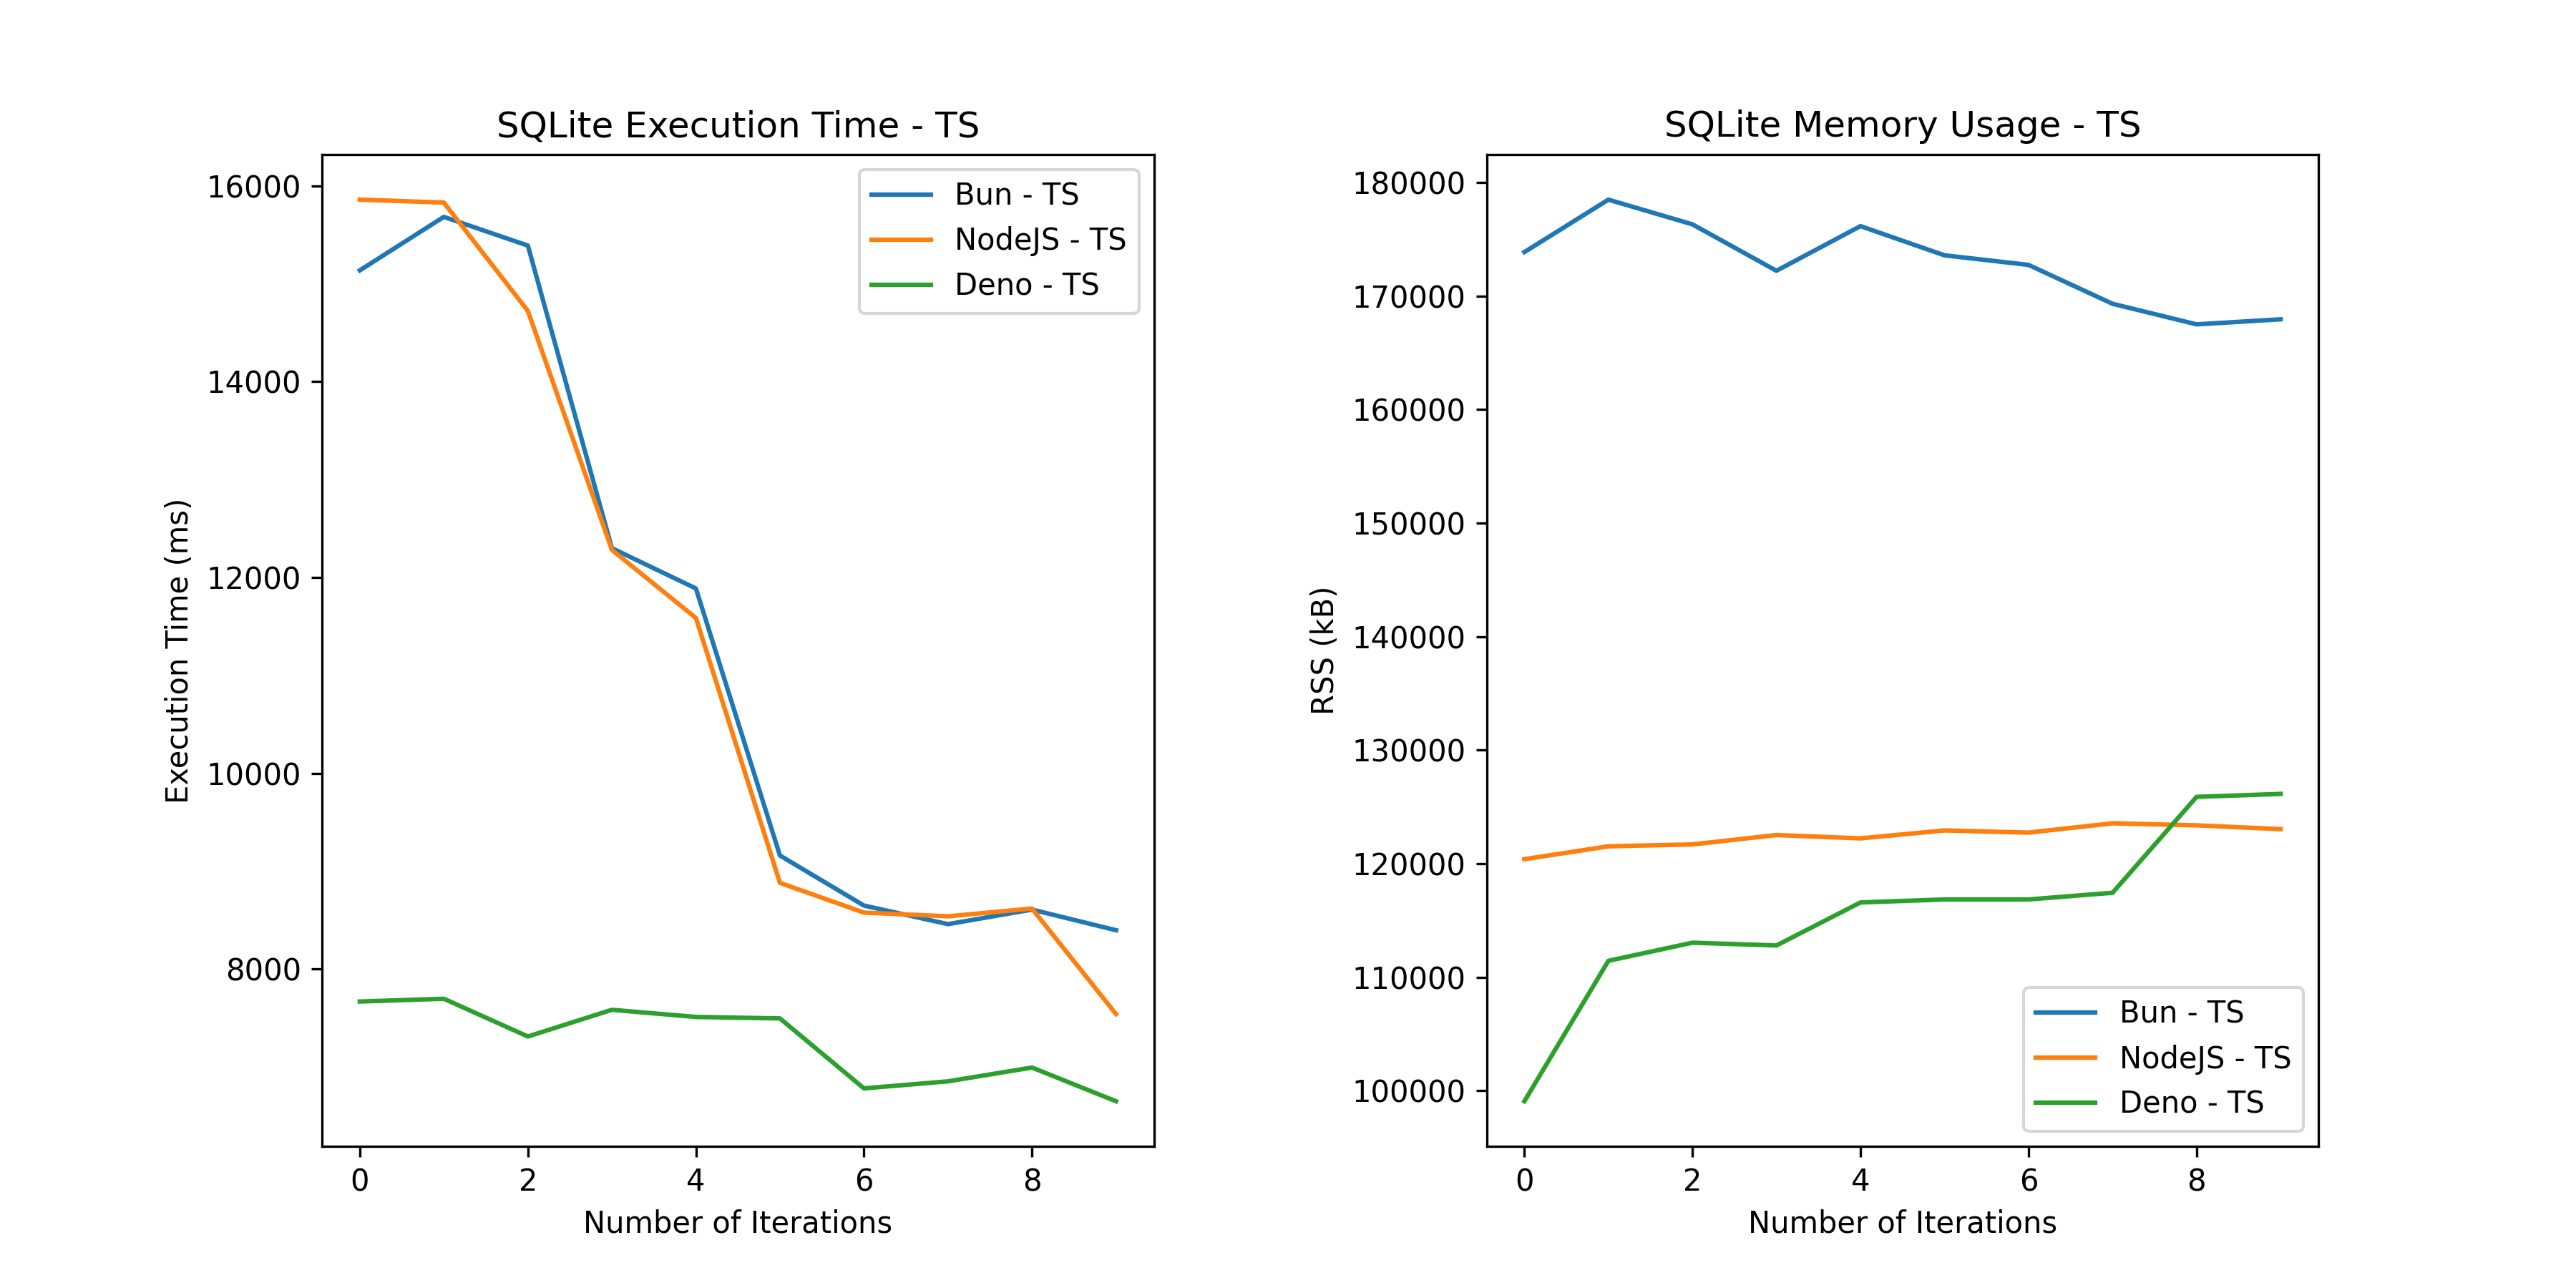
\includegraphics[width=0.68\textwidth]{Figures/database/sqlite_10_1000_ts.png}
  \caption{Wyniki eksperymentów dla testu bazy danych 10 iteracji oraz 1000 rekordów - po lewej czas wykonania jednorazowego testu w milisekundach, po prawej ilość zajmowanej pamięci w kilobajtach (kB)}
  \label{fig:database_e1_ts}
\end{figure}

Na rysunku \ref{fig:database_e2_js} przedstawiono wyniki eksperymentów dla testu bazy danych dla 100 iteracji oraz 1000 rekordów napisanego w języku JavaScript. Na wykresie przedstawiono czas wykonania jednorazowego testu w milisekundach oraz ilość zajmowanej pamięci w kilobajtach (kB).

\begin{figure}[H]
  \centering
  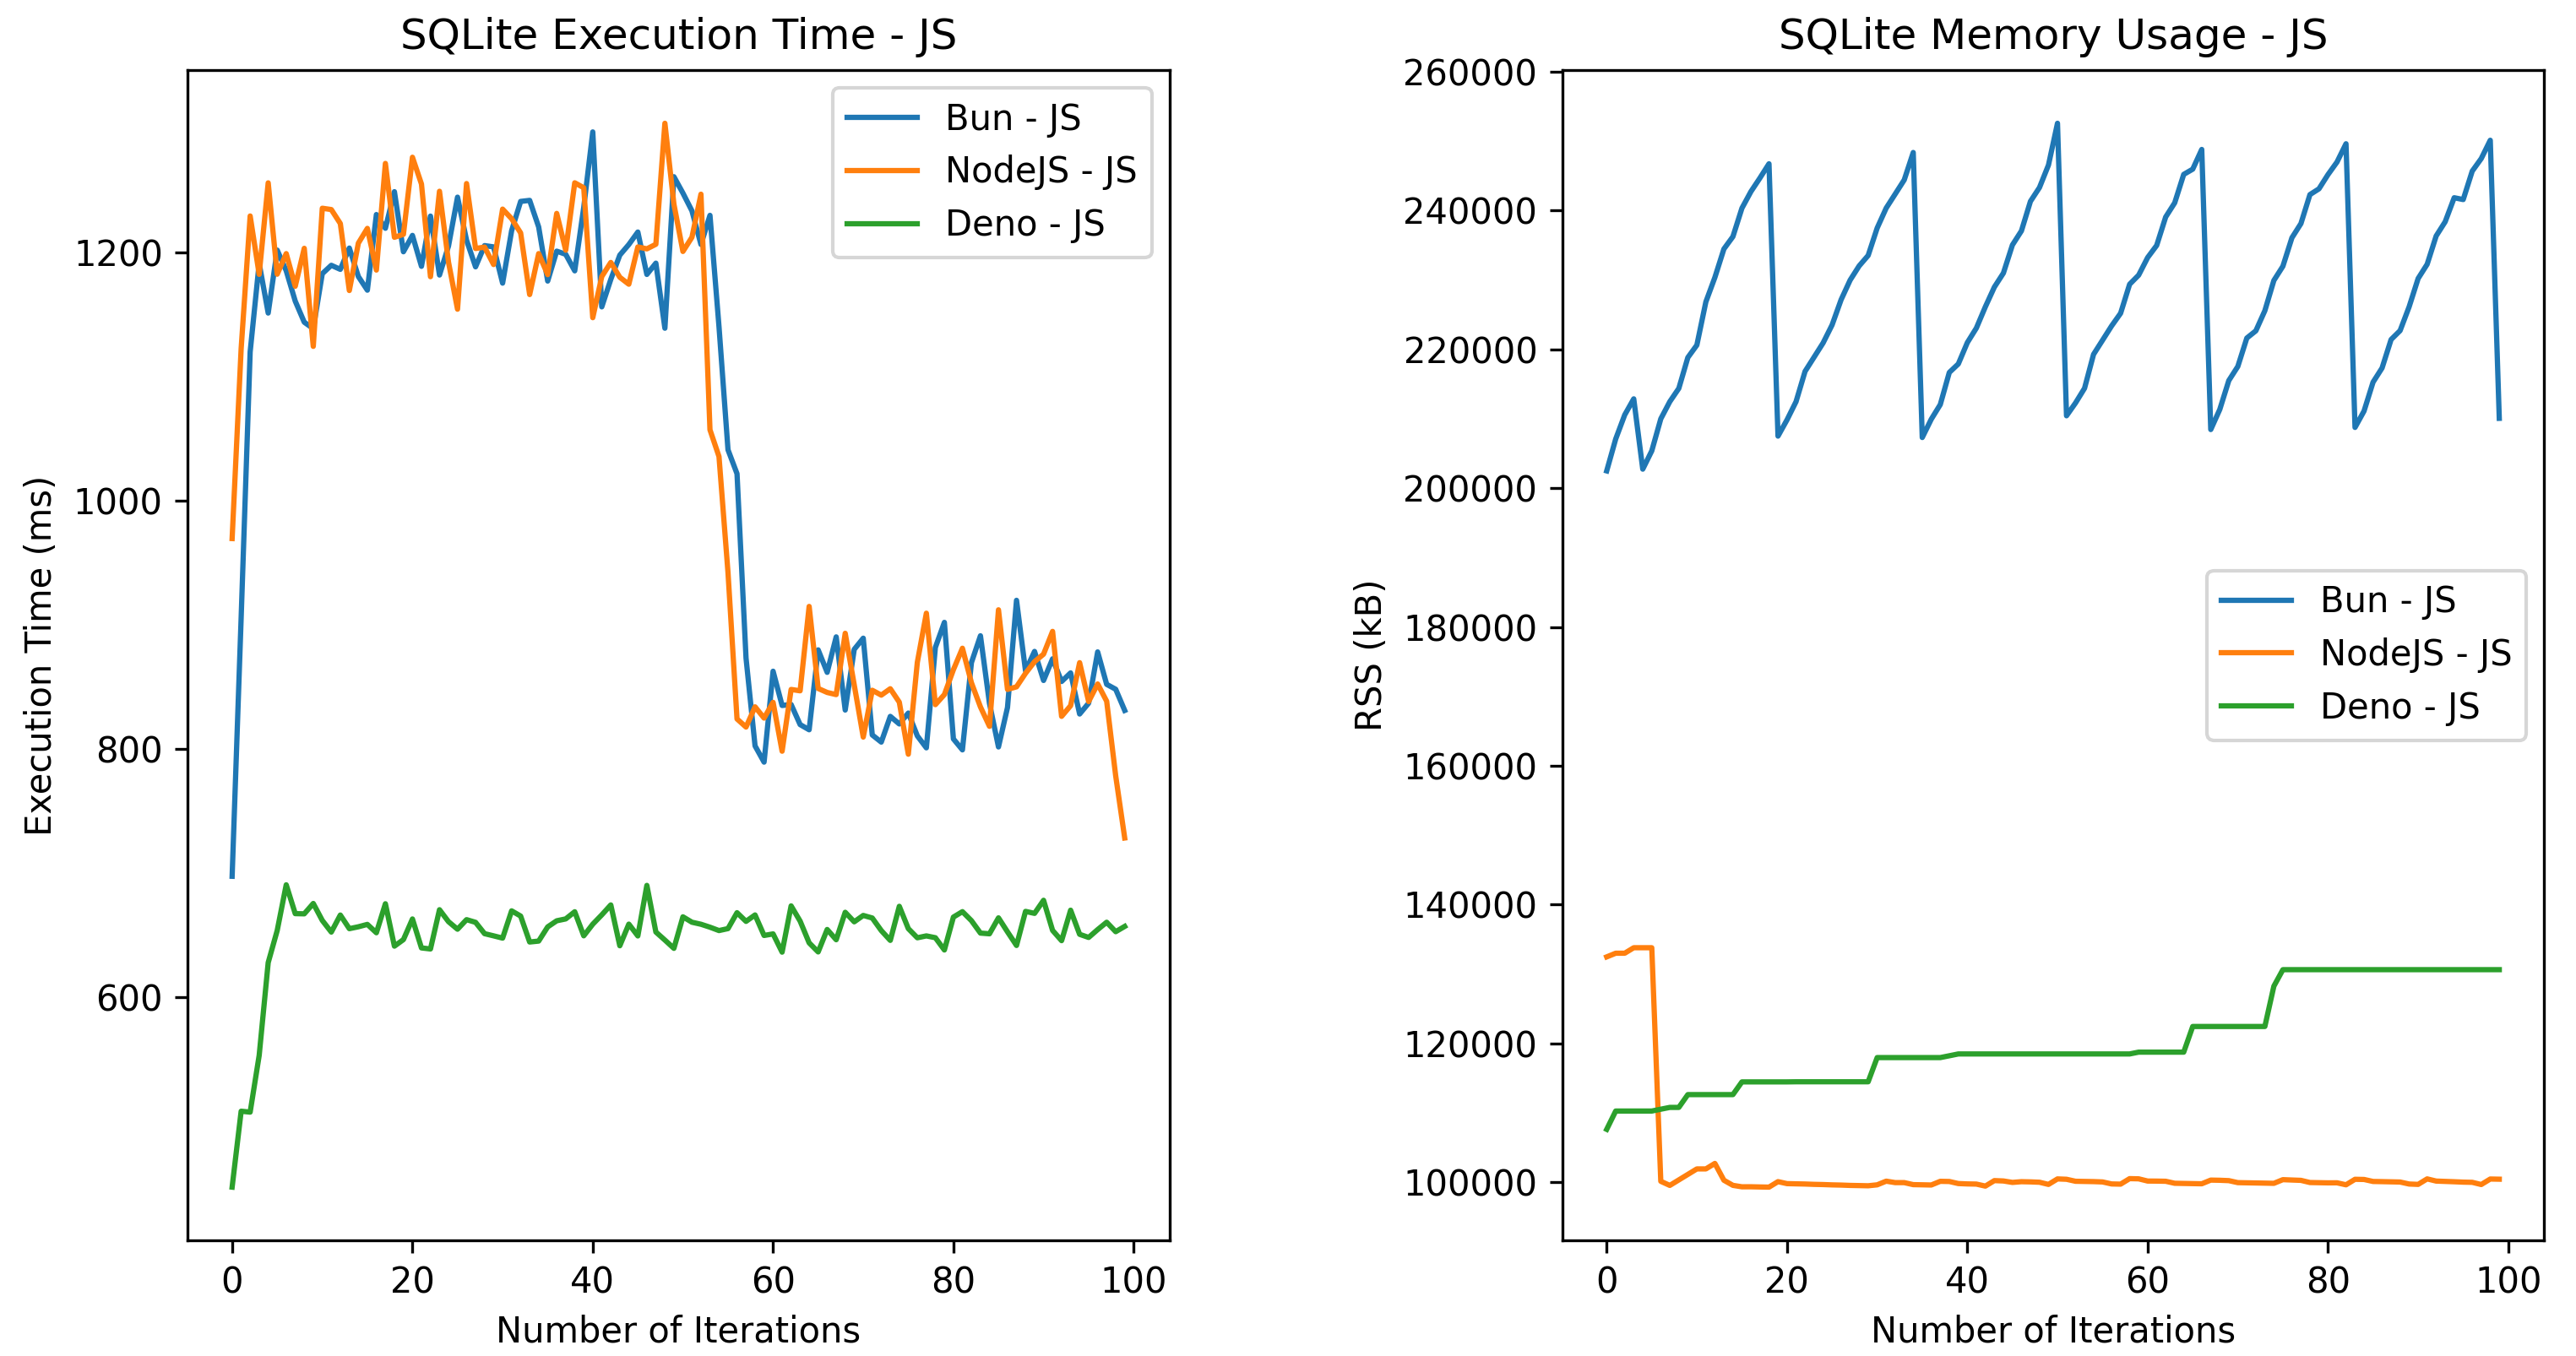
\includegraphics[width=0.68\textwidth]{Figures/database/sqlite_100_1000_js.png}
  \caption{Wyniki eksperymentów dla testu bazy danych 100 iteracji oraz 1000 rekordów - po lewej czas wykonania jednorazowego testu w milisekundach, po prawej ilość zajmowanej pamięci w kilobajtach (kB)}
  \label{fig:database_e2_js}
\end{figure}

Na rysunku \ref{fig:database_e2_ts} przedstawiono wyniki eksperymentów dla testu bazy danych dla 100 iteracji oraz 1000 rekordów napisanego w języku TypeScript. Na wykresie przedstawiono czas wykonania jednorazowego testu w milisekundach oraz ilość zajmowanej pamięci w kilobajtach (kB).

\begin{figure}[H]
  \centering
  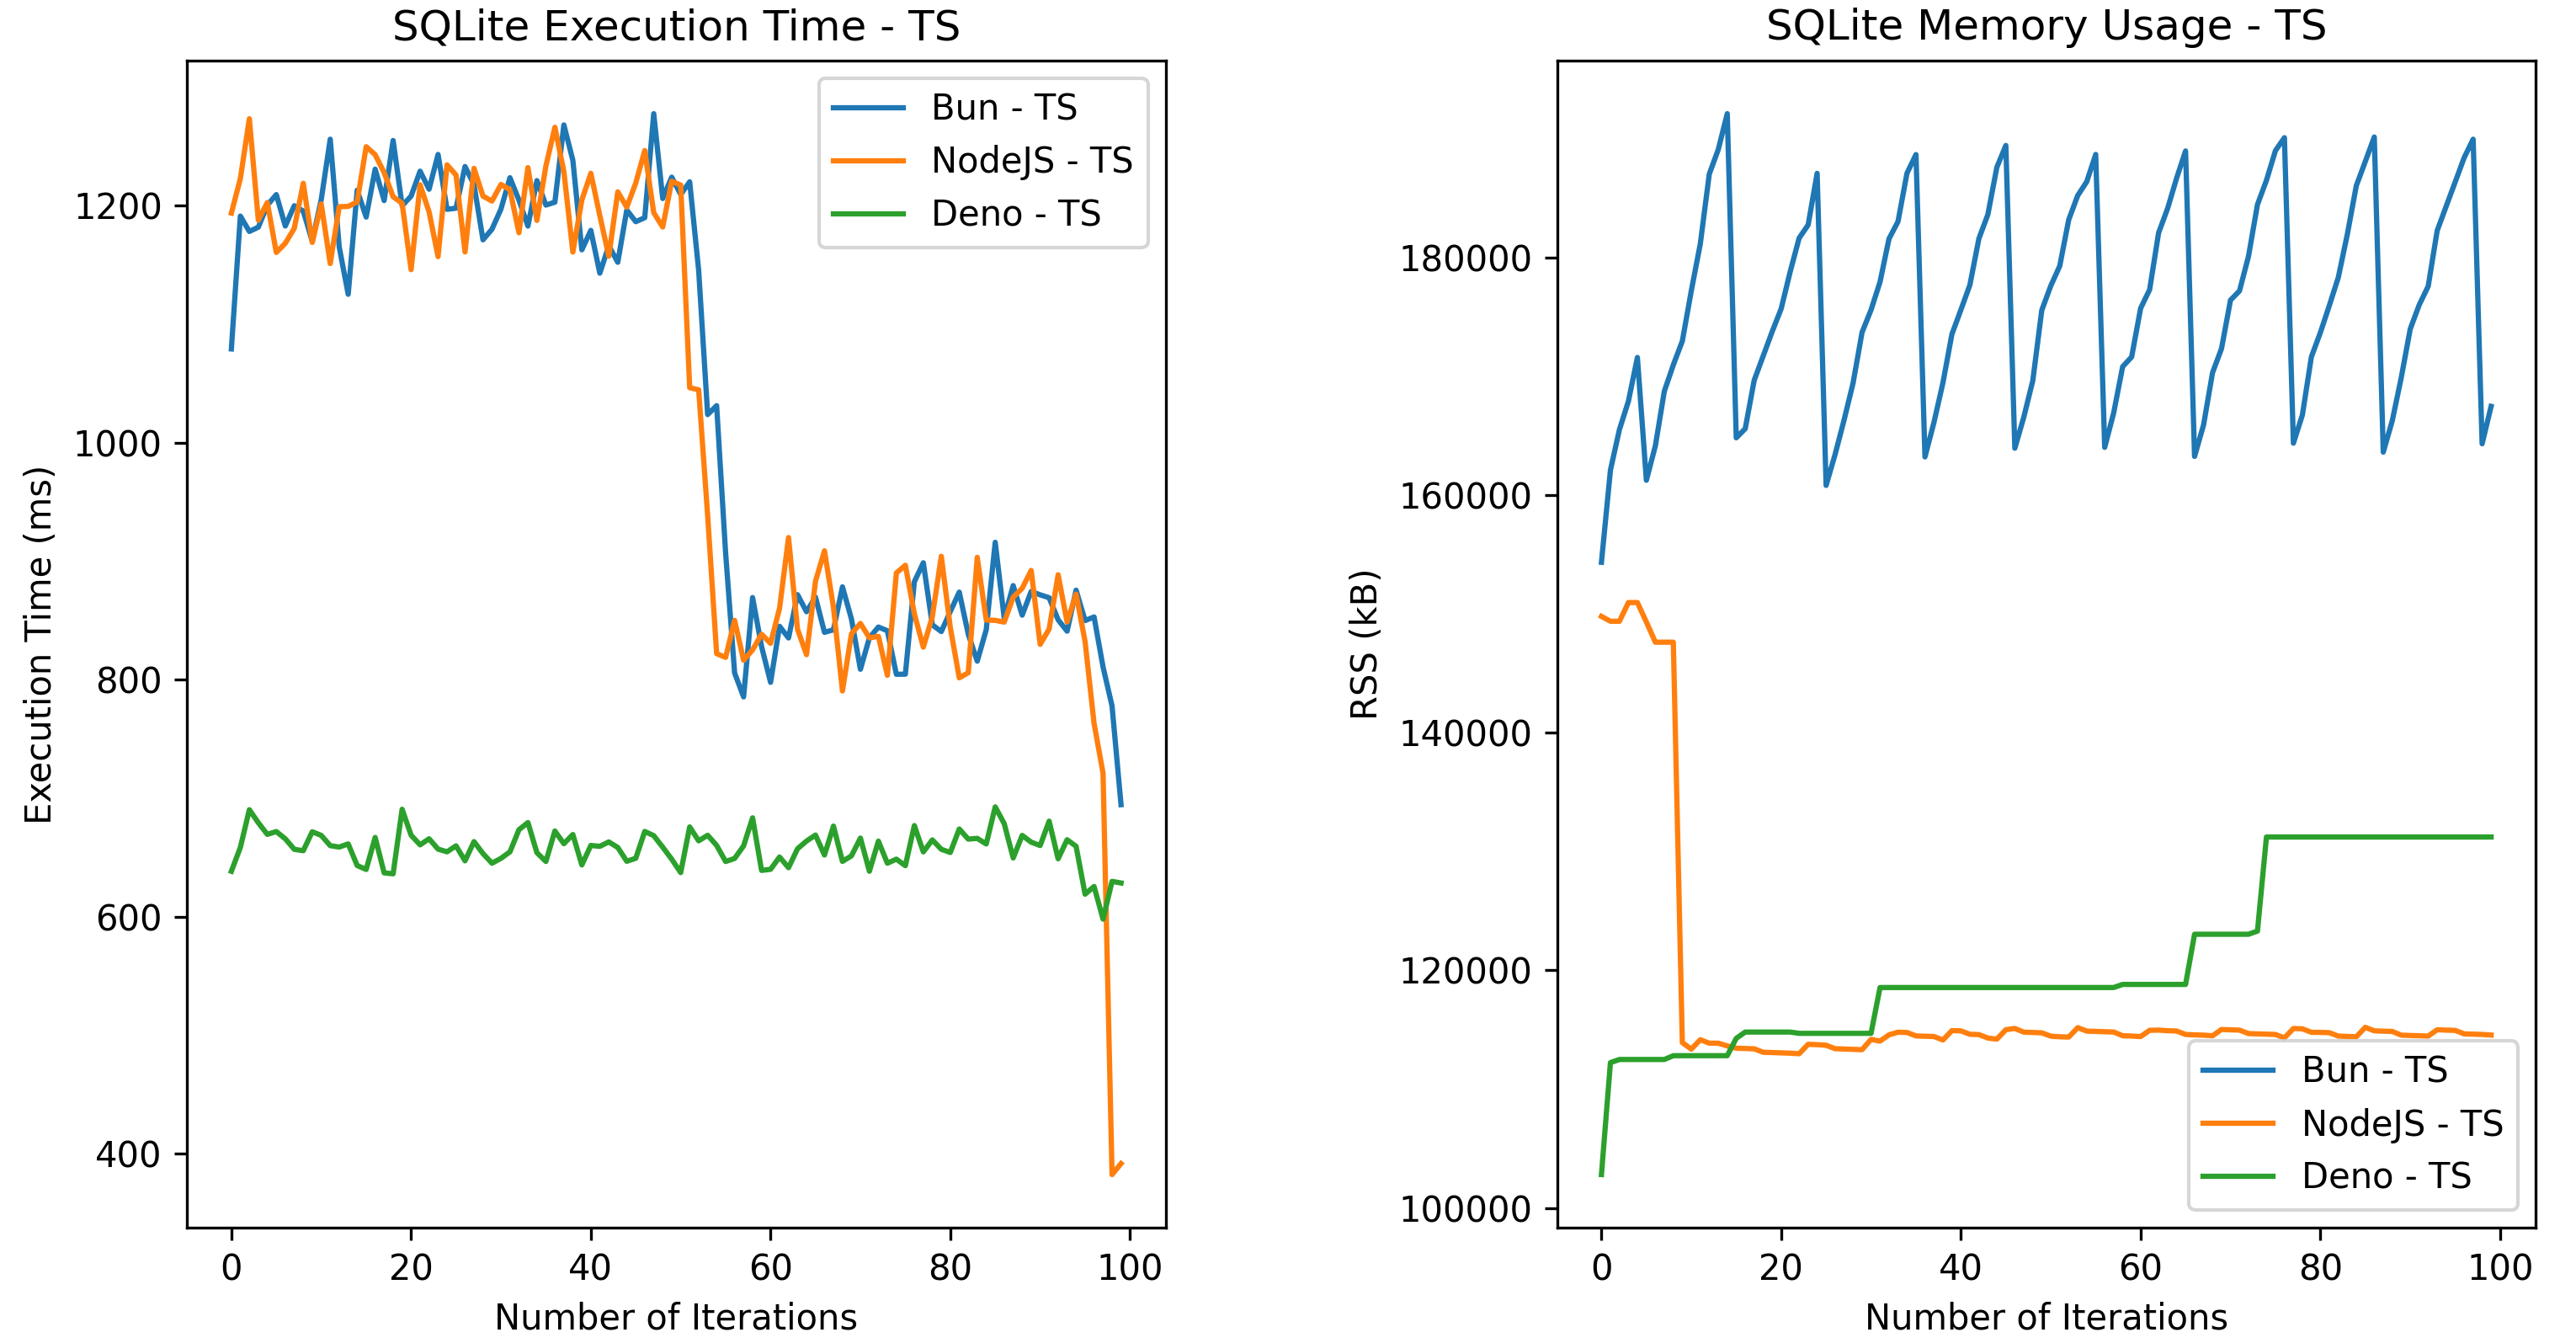
\includegraphics[width=0.68\textwidth]{Figures/database/sqlite_100_1000_ts.png}
  \caption{Wyniki eksperymentów dla testu bazy danych 100 iteracji oraz 1000 rekordów - po lewej czas wykonania jednorazowego testu w milisekundach, po prawej ilość zajmowanej pamięci w kilobajtach (kB)}
  \label{fig:database_e2_ts}
\end{figure}